
\documentclass[xcolor=x11names,compress, aspectratio=169]{beamer}

%\documentclass[xcolor=x11names,compress, handhouts]{beamer}

%% General document
\usepackage{graphicx, subfig}
%% Beamer Layout
\useoutertheme[subsection=false,shadow]{miniframes}
\useinnertheme{default}
\usefonttheme{serif}
\usepackage{palatino}

%%%%%%% Mes Packages %%%%%%%%%%%%%%%%
\usepackage[french]{babel}
%\usepackage[T1]{fontenc}
\usepackage[latin1]{inputenc}
\usepackage{color}
\usepackage{dsfont} % Pour indicatrice
\usepackage{url}
\usepackage{multirow}
\usepackage{ulem}  % strike out text

%remove the icon
\setbeamertemplate{bibliography item}{}

%remove line breaks
\setbeamertemplate{bibliography entry title}{}
\setbeamertemplate{bibliography entry location}{}
\setbeamertemplate{bibliography entry note}{}

%% ------ MEs couleurs --------
\definecolor{vert}{rgb}{0.1,0.7,0.2}
\definecolor{brique}{rgb}{0.7,0.16,0.16}
\definecolor{gris}{rgb}{0.7, 0.75, 0.71}
\definecolor{twitterblue}{rgb}{0, 0.42, 0.58}
\definecolor{airforceblue}{rgb}{0.36, 0.54, 0.66}
\definecolor{siap}{RGB}{3,133, 168}


%%%%%%%%%%%%%%%%% BEAMER PACKAGE %%%%%%%
\setbeamercolor{itemize item}{fg=siap}
%\setbeamercolor{itemize subitem}{fg=blue}
%\setbeamercolor{itemize subsubitem}{fg=cyan}

%\setbeamertemplate{itemize item}[square]
%\setbeamertemplate{itemize subitem}[circle]
%\setbeamertemplate{itemize subsubitem}[triangle]



\setbeamerfont{title like}{shape=\scshape}
\setbeamerfont{frametitle}{shape=\scshape}

\setbeamercolor*{lower separation line head}{bg=DeepSkyBlue4}
\setbeamercolor*{normal text}{fg=black,bg=white}
\setbeamercolor*{alerted text}{fg=siap}
\setbeamercolor*{example text}{fg=black}
\setbeamercolor*{structure}{fg=black}
\setbeamercolor*{palette tertiary}{fg=black,bg=black!10}
\setbeamercolor*{palette quaternary}{fg=black,bg=black!10}

\renewcommand{\(}{\begin{columns}}
\renewcommand{\)}{\end{columns}}
\newcommand{\<}[1]{\begin{column}{#1}}
\renewcommand{\>}{\end{column}}

%% Path for the graphs
%\graphicspath{{../Graphics/}{../Graphics/FromPdf/}{../../../../Visualisation/Presentations/Graphics/}{../../Visualisation/Presentations/Graphics/} {../R-Codes/JobSatisfaction_files/figure-latex/}{../R-Codes/Unused_files/figure-latex/}}



% Path for the graphs
\graphicspath{
{Graphics/}
}


%remove navigation symbols
\setbeamertemplate{navigation symbols}{}



% Natbib for clean bibliography
\usepackage[comma,authoryear]{natbib}

%% General document
\usepackage{graphicx, subfig}
%% Beamer Layout
\useoutertheme[subsection=false,shadow]{miniframes}
\useinnertheme{default}
\usefonttheme{serif}
\usepackage{palatino}

%%%%%%% Mes Packages %%%%%%%%%%%%%%%%
\usepackage[french]{babel}
\usepackage[T1]{fontenc}
\usepackage{color}
\usepackage{dsfont} % Pour indicatrice
\usepackage{url}
\usepackage{multirow}

\usepackage{bibentry}  %  for citing full references
%remove the icon
\setbeamertemplate{bibliography item}{}


%remove navigation symbols
\setbeamertemplate{navigation symbols}{}


\title{\textcolor{siap}{JICA-TAPOS}}
\subtitle{\textcolor{siap}{\large{Data Visualization - Descriptive \& Inferential  Statistics}}}
\author{Christophe Bontemps}
\institute{\large{\emph{Statistical Institute for Asia and the Pacific} } \\
    
\includegraphics[height=10ex]{SIAP_logo_Big.png}}
\date{}


\begin{document}

\begin{frame}
\titlepage
\end{frame}


\begin{frame}
\begin{center}
\textcolor{brique}{{\huge H
\includegraphics[height=0.4cm]{LieRed.png}w  \textcolor{brique}{[Not]} To Lie With Graphics?}}
%\textcolor{brique}{\huge{How [Not] To Lie With Graphics}}
\vspace{0.5cm}

\textcolor{siap}{\textit{Christophe Bontemps,}\\ UN  SIAP}
\vspace{0.5cm}


\includegraphics[height=0.10\textwidth]{SIAP_logo_Big.png}

\end{center}

\end{frame}
\section{Foreword}



\begin{frame} % Cover slide
\frametitle{\textcolor{brique}{[-Foreword-]}}
\begin{center}

\huge{\textcolor{siap}{What is Data Visualisation about?}}

\vspace{0.5cm}
\large{\textcolor{brique}{( \textit{Do you remember from day 1?})}}
\end{center}
\end{frame}


\begin{frame} % Cover slide
\frametitle{\textcolor{brique}{[-Foreword-]}: What's Data Visualisation?}
\begin{center}
What do you see?\\

  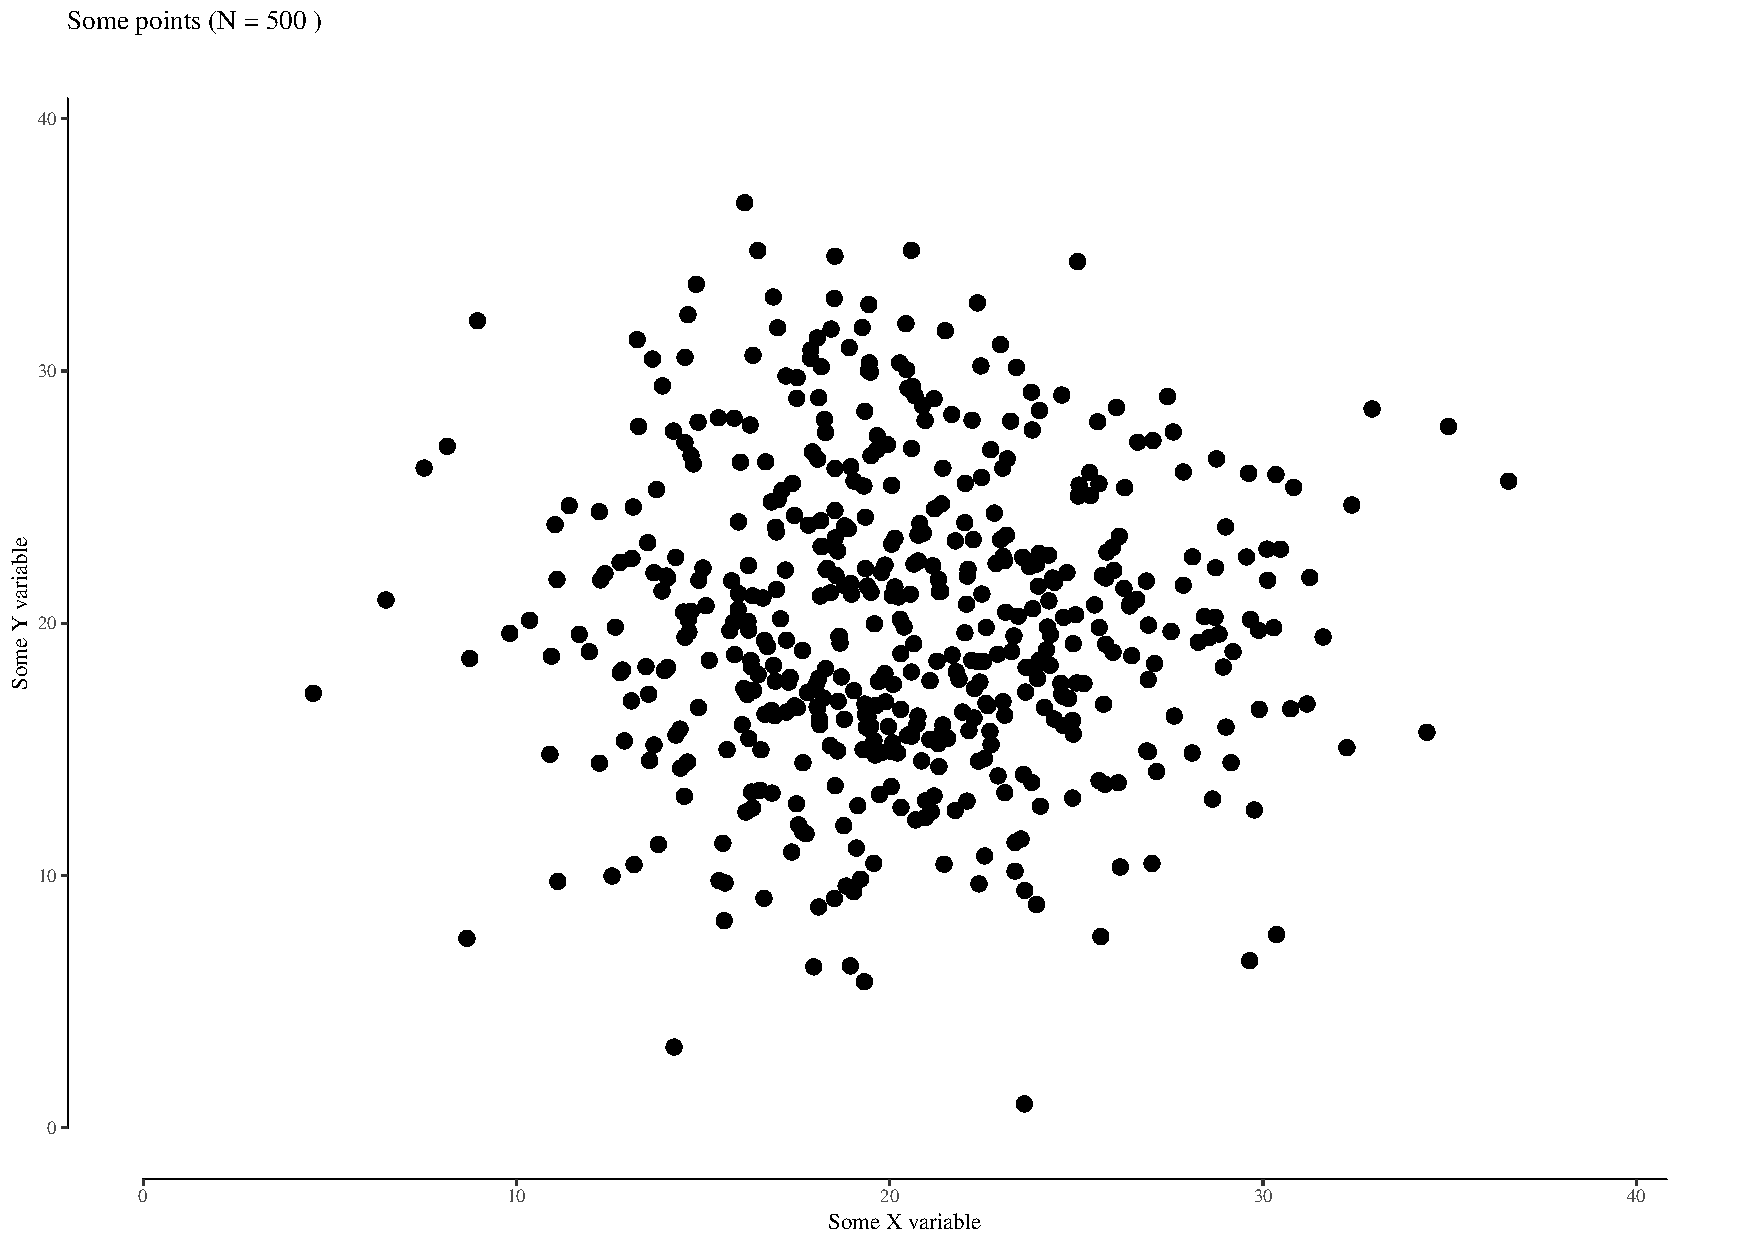
\includegraphics[width = 0.6\textwidth]{RandomPoints.pdf}
\end{center}
\end{frame}


\begin{frame} % Cover slide
\frametitle{\textcolor{brique}{[-Foreword-]}: What's Data Visualisation?}
 \begin{center}
 And here, what do you see?\\
  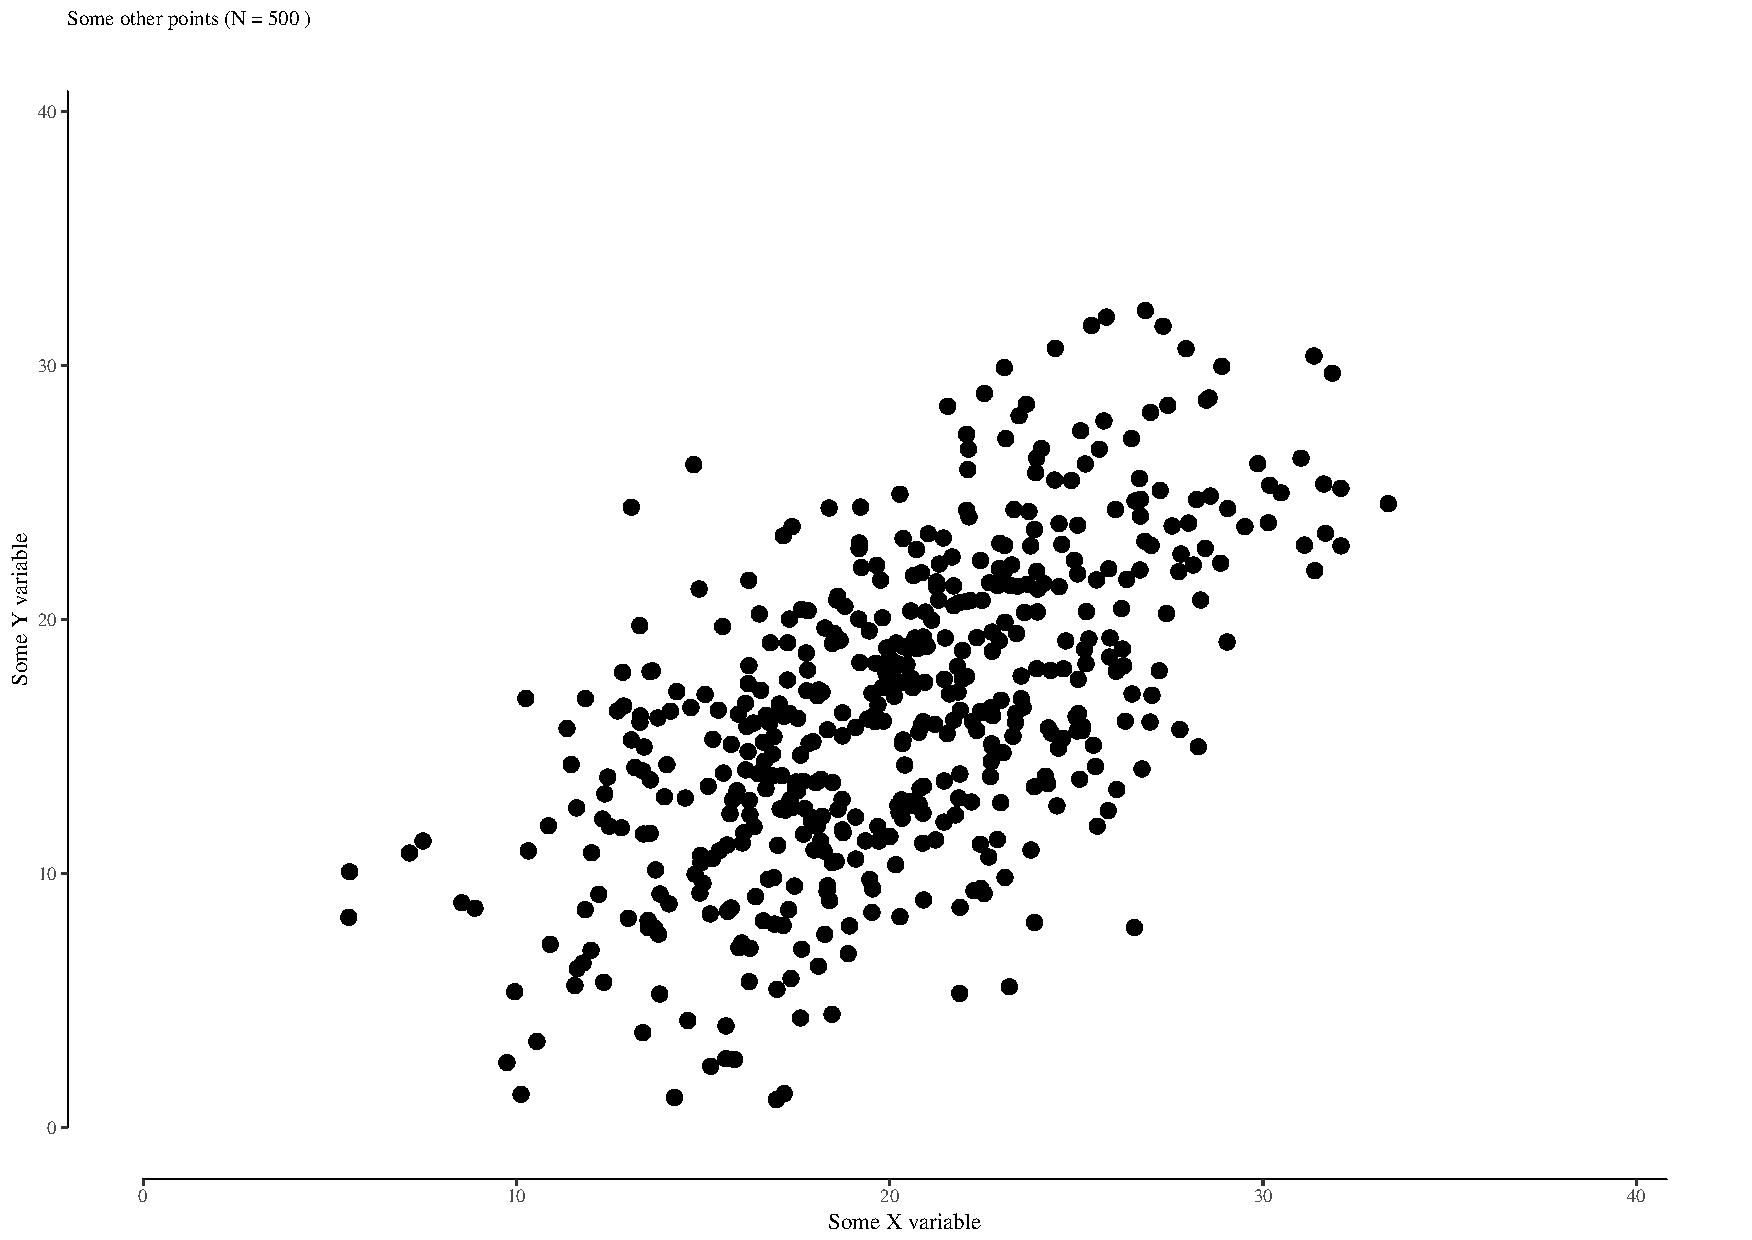
\includegraphics[width = 0.6\textwidth]{LinearPoints1.pdf}
\end{center}
\end{frame}

\begin{frame} % Cover slide
\frametitle{``Data visualisation'' as a statistical test }
 \begin{itemize}
  \item<+->[] 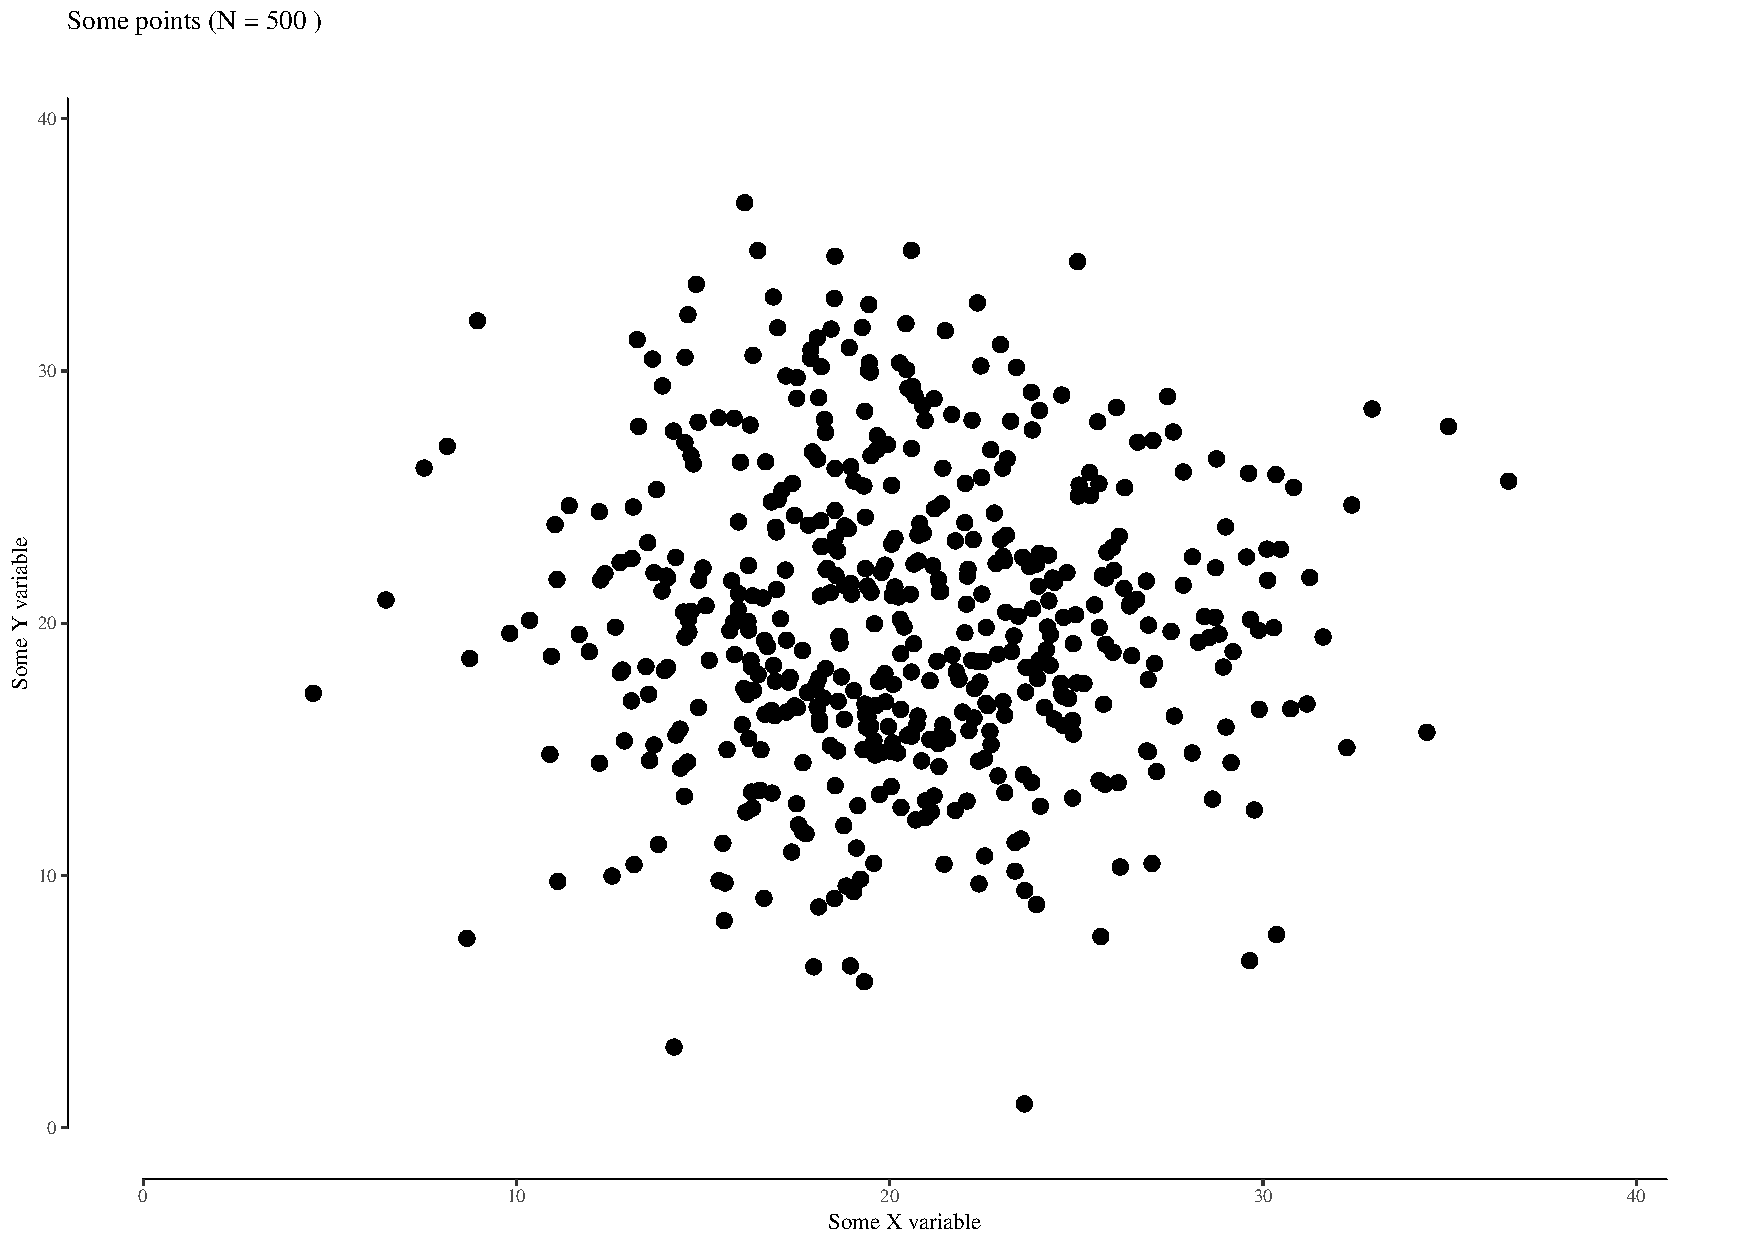
\includegraphics[width = 0.2\textwidth]{RandomPoints.pdf}
            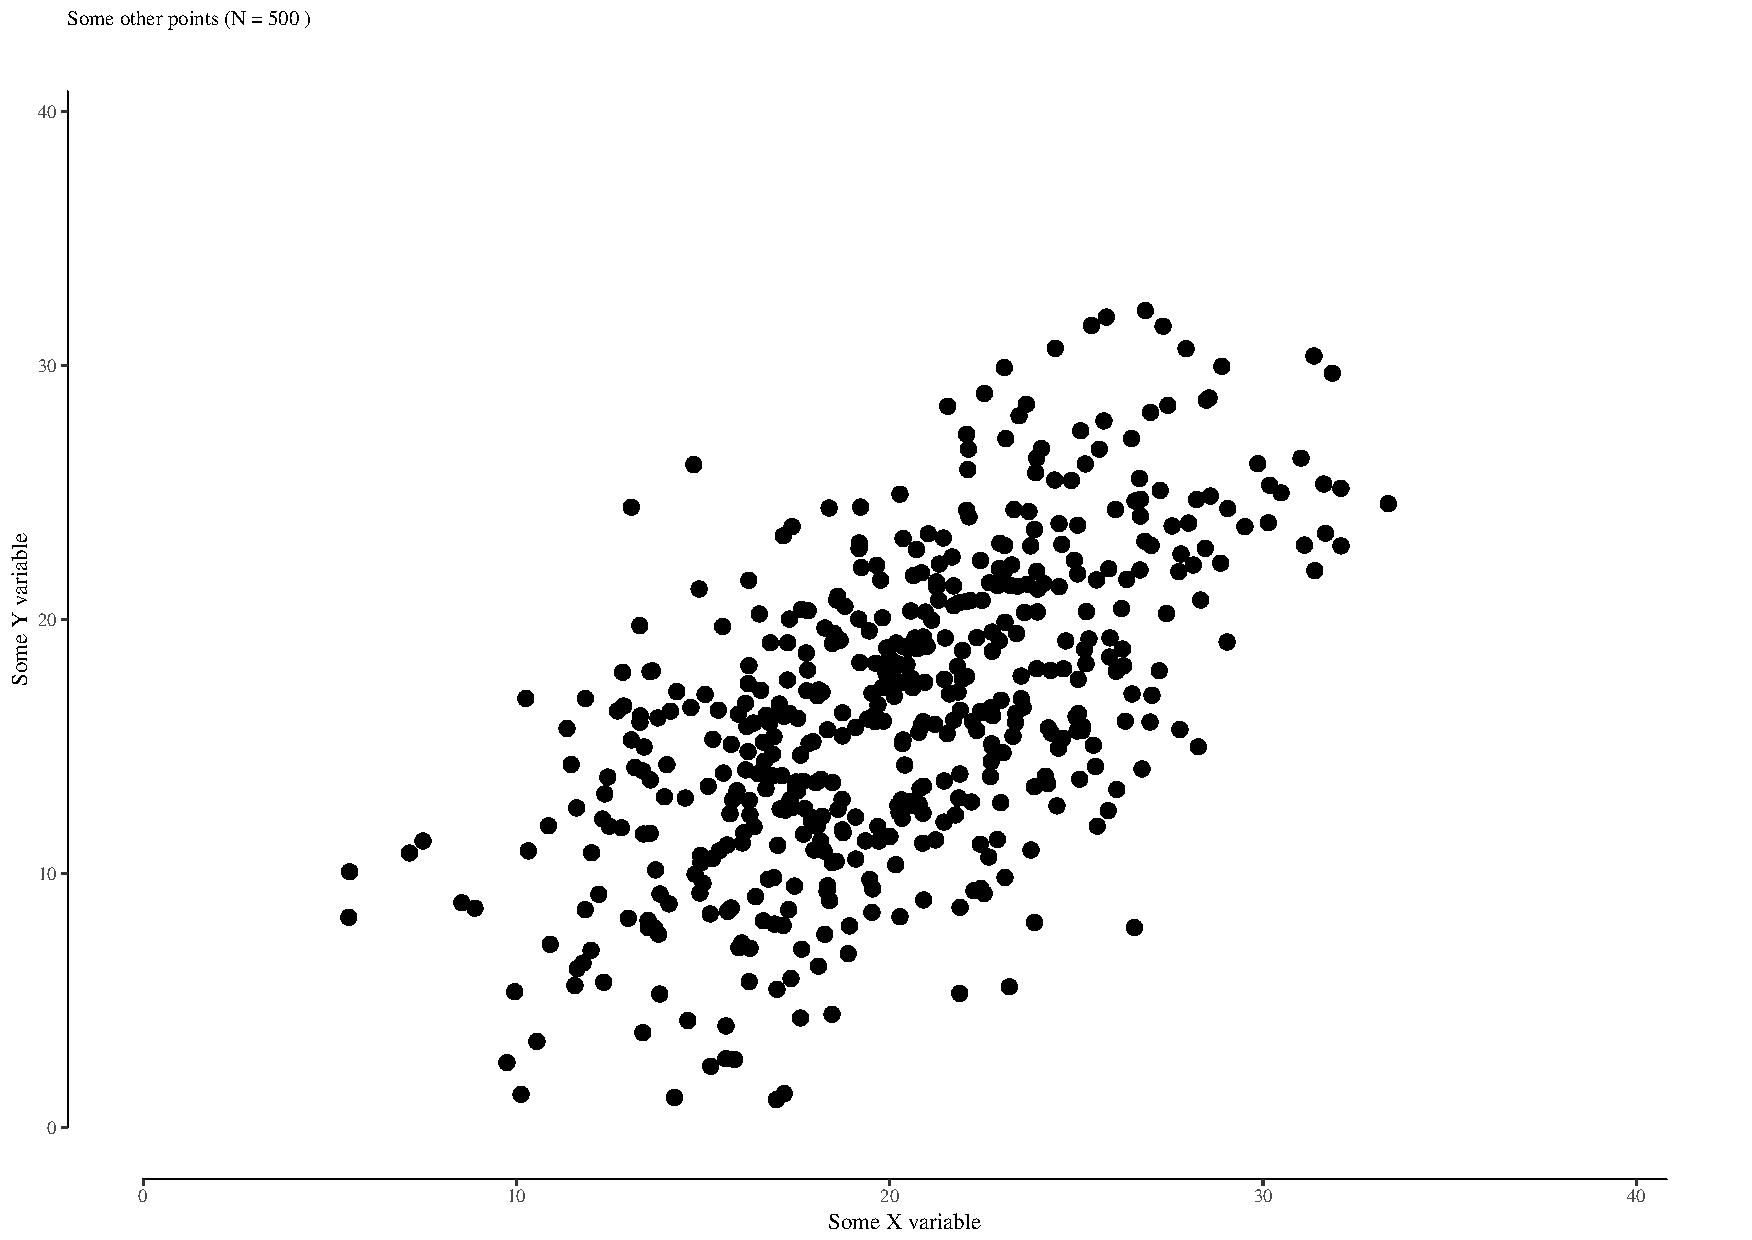
\includegraphics[width = 0.2\textwidth]{LinearPoints1.pdf}
            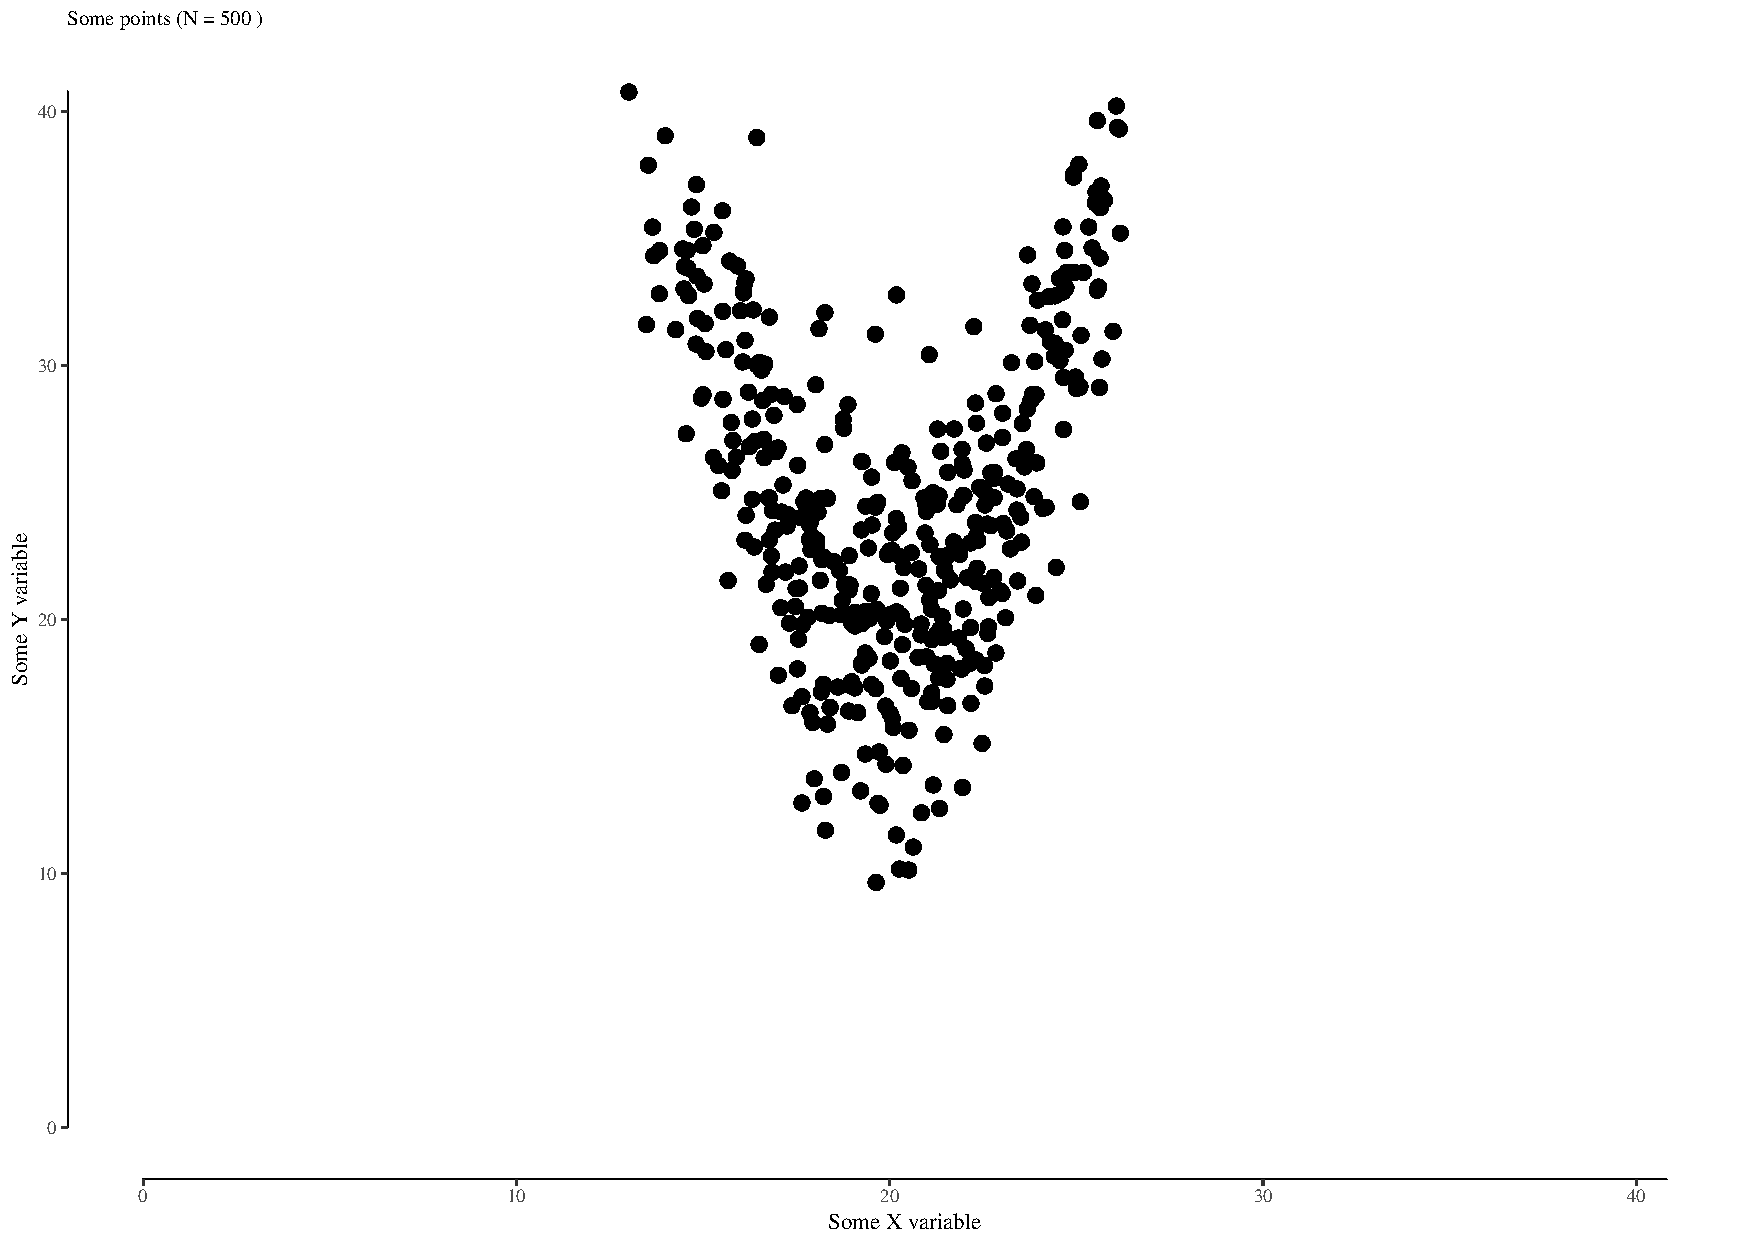
\includegraphics[width = 0.2\textwidth]{UshapedPoints.pdf}
            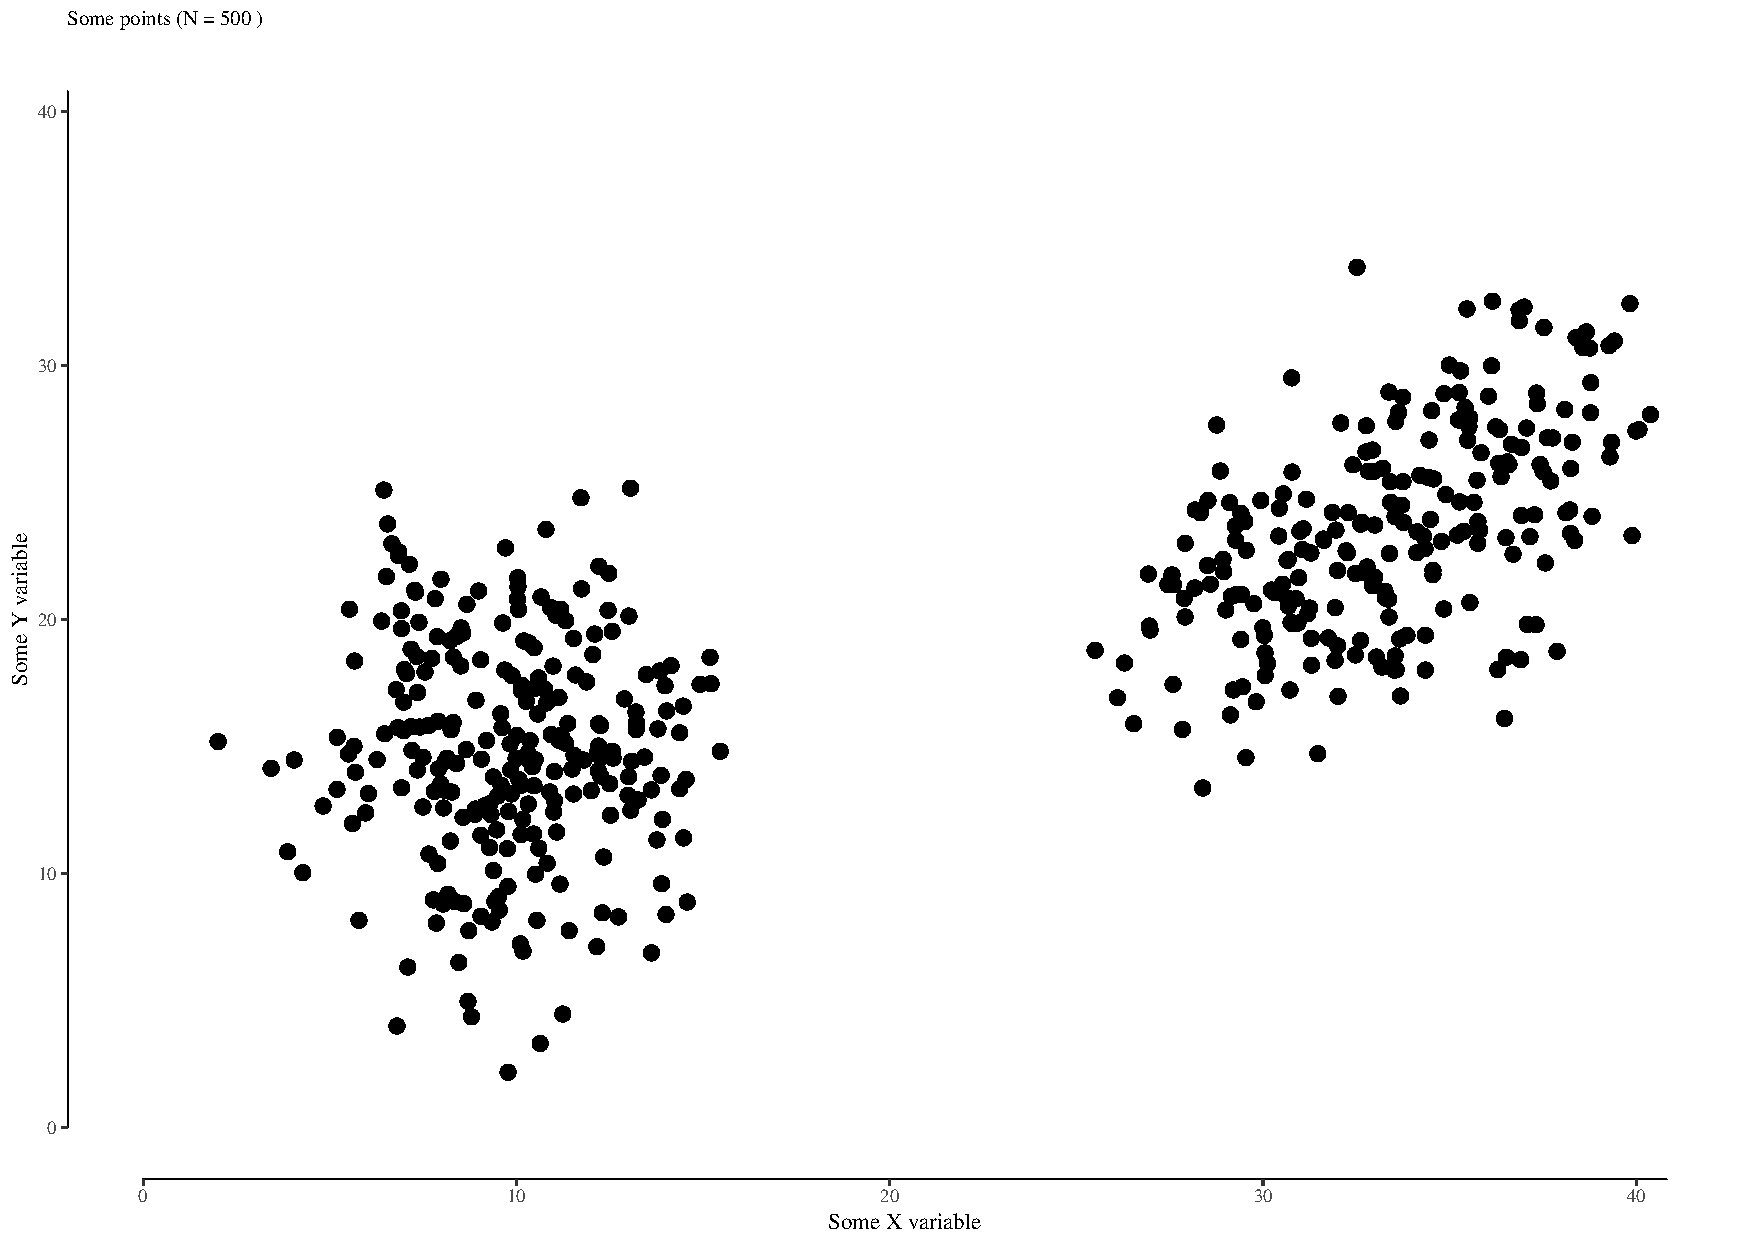
\includegraphics[width = 0.2\textwidth]{GroupsPoints.pdf}
  \item<+->[] {\centering \textit{`` The human eye acts is a broad feature detector and general statistical test''. \cite{Buja2009}}}
  \item<+->[\textbf{Test:}] $H_0$ : \{There is "nothing"  \} = \{\textbf{No} relation\}
  \item<+->[] $H_1$ : \{ There is "something" \} = \{There is \textbf{some} relation (Correlation, linearity, heterogeneity, groups..) \}
 \end{itemize}
\end{frame}



\begin{frame} % Cover slide
\frametitle{\textcolor{brique}{[-Foreword-]}: What's Data Visualisation?}
\begin{center}

\huge{\textcolor{siap}{Data Visualization is about\\   (fair!)} \textcolor{brique}{comparisons}}
\end{center}
\end{frame}

\begin{frame} % Cover slide
\frametitle{\textcolor{brique}{[- What we do: -]}: \textbf{Implicit} comparisons}
\begin{center}
\begin{itemize}
  \only<1>{What does this curves tells you ? }
  \only<1>{ 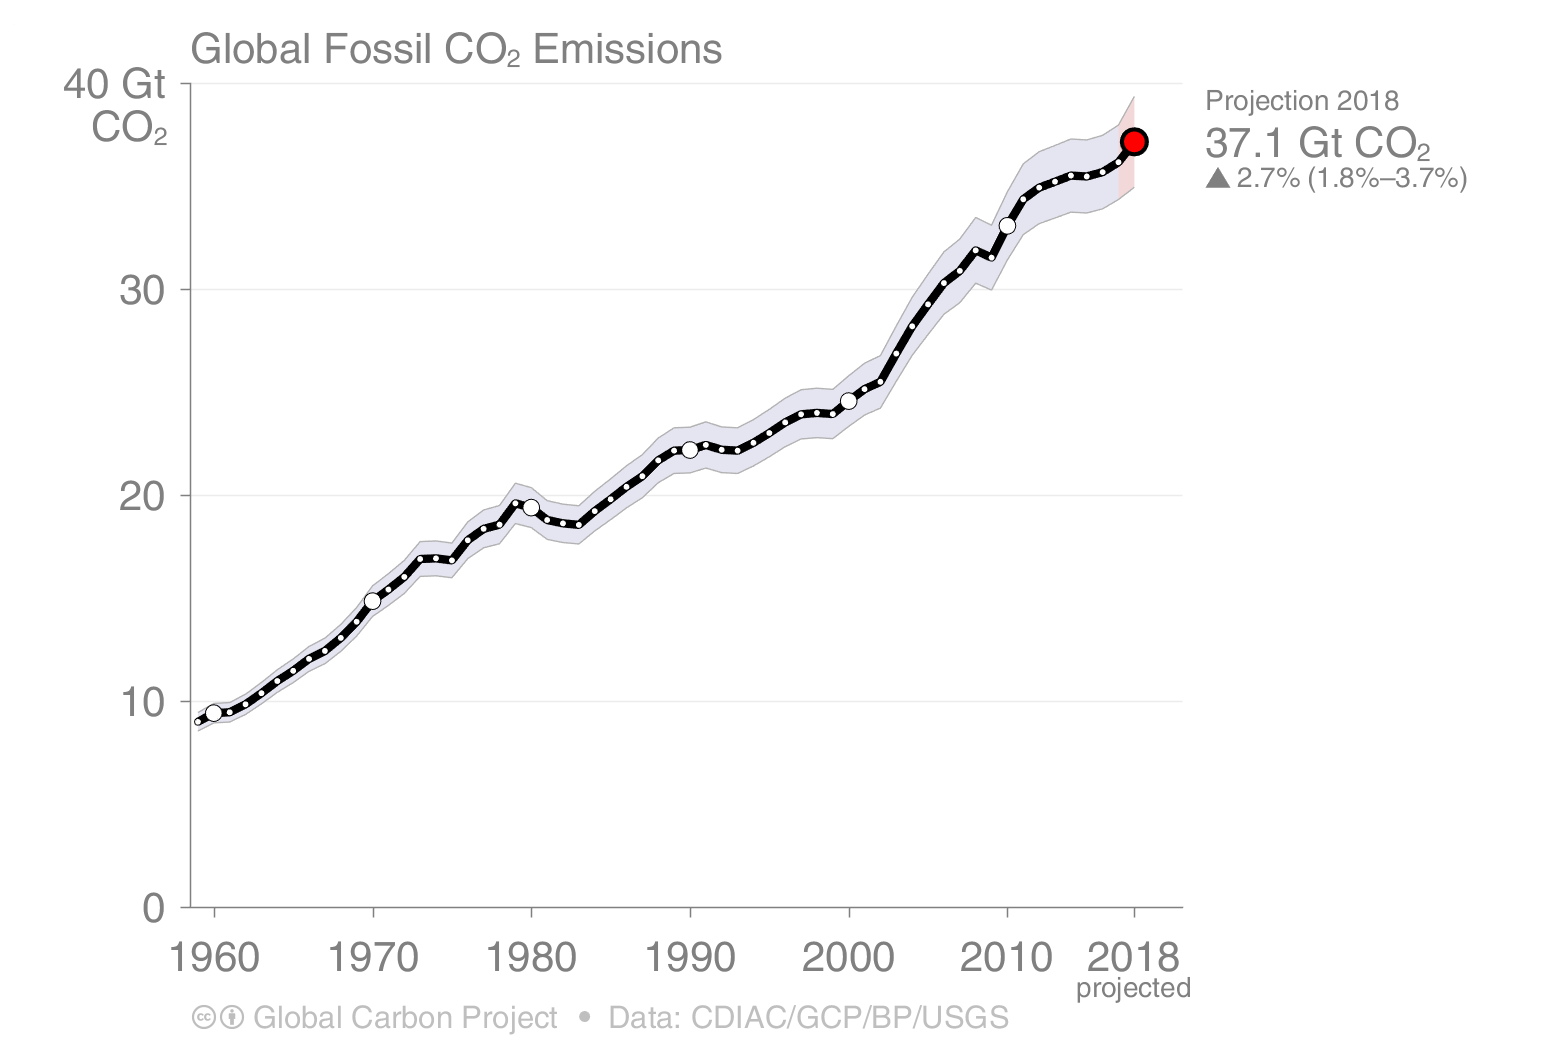
\includegraphics[width = 0.7\textwidth]{FossilFuel_and_Cement_emissions_1959.png}}
\end{itemize}
\end{center}
\end{frame}



\begin{frame} % Cover slide
\frametitle{\textcolor{brique}{[- What we do: -]}:  \textbf{Explicit} comparisons }

\begin{center}
\begin{itemize}
  \only<1>{We compare: \textcolor{brique}{\textbf{surfaces}... }}
  \only<1>{ 
\includegraphics[width = 0.8\textwidth]{DesignNumbers-18.png}}
  \only<2>{ \textcolor{brique}{\textbf{lines}... } \\ \vspace{0.5cm} }
  \only<2>{}
  \only<2>{ 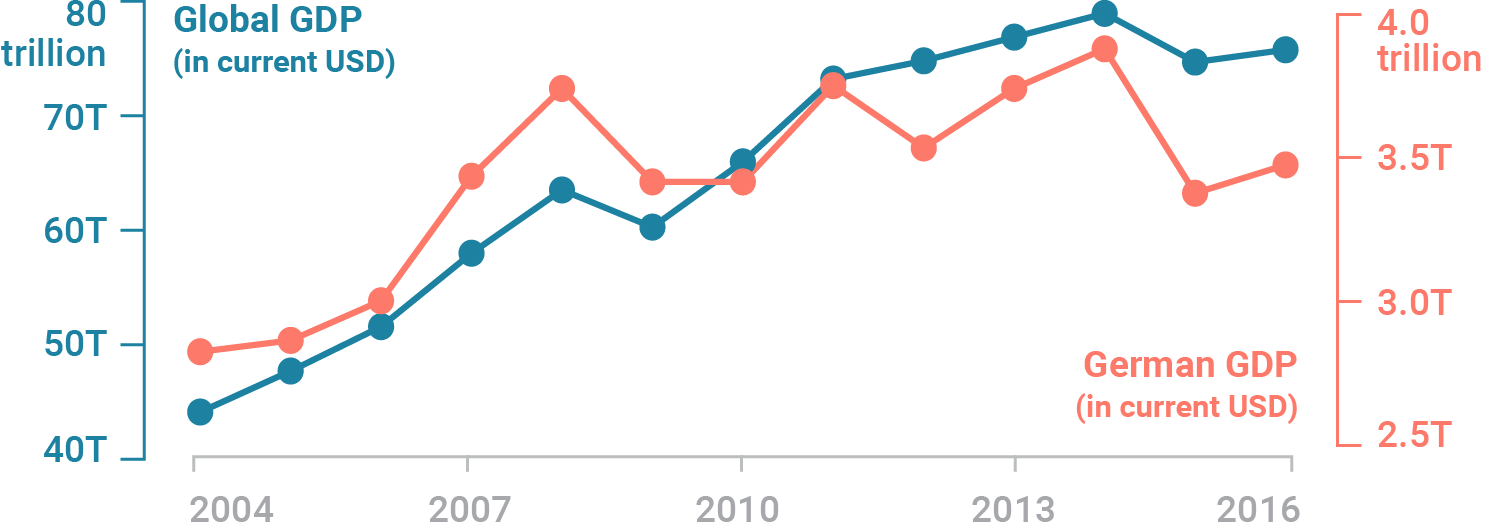
\includegraphics[width = 0.8\textwidth]{LCRost-dualaxis1.png}}
  \only<3>{\textcolor{brique}{\textbf{lengths}...} \\ }
  \only<3>{ 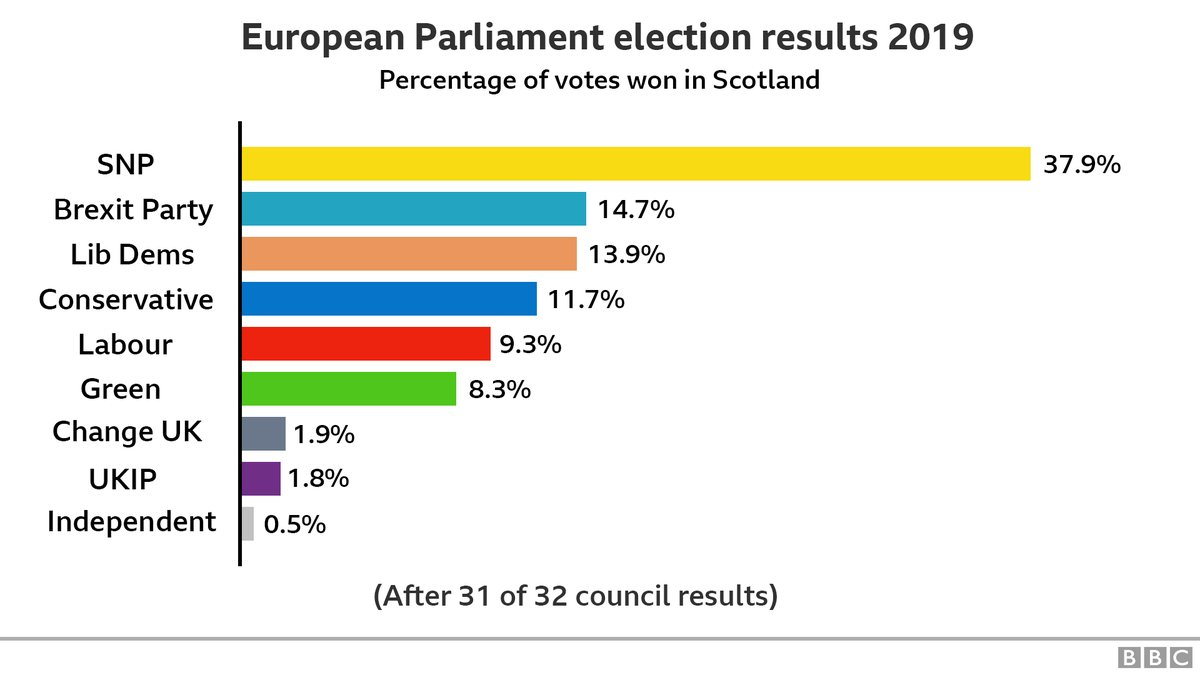
\includegraphics[width = 0.8\textwidth]{BBC-EUElectionOriginal.jpg}}
  \only<4>{\textcolor{brique}{\textbf{colors}...}  \\ }
  \only<4>{ 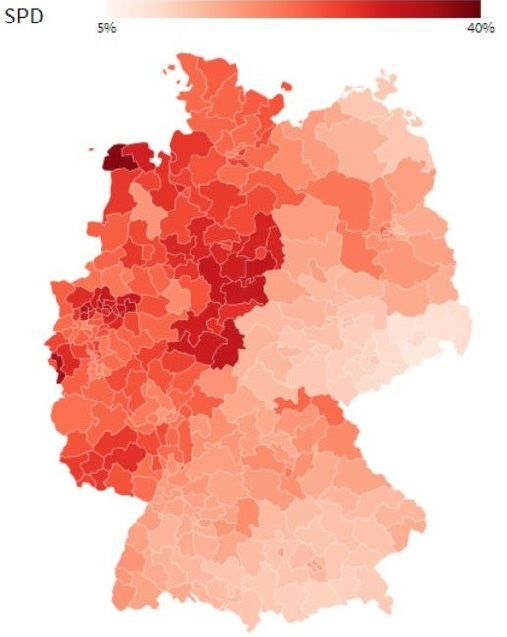
\includegraphics[width = 0.35\textwidth]{GermanElectionsSPD.JPG}}
\end{itemize}
\end{center}
\end{frame}

%
%
%\begin{frame} % Cover slide
%%\frametitle{\textcolor{brique}{[-  -]}: }
%\begin{center}
%\begin{Huge}
%  What if all of this was a lie?\\
%\end{Huge}
%
%\vspace{0.5cm}
%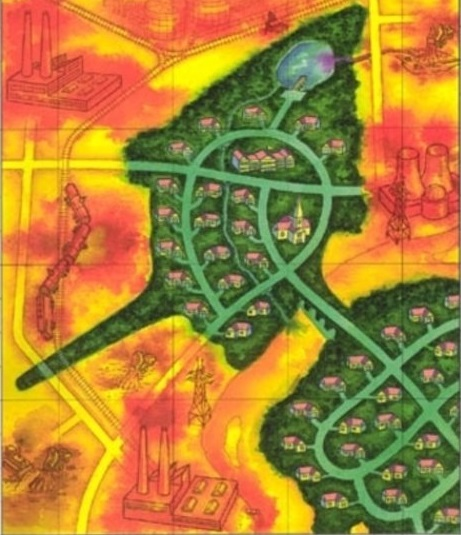
\includegraphics[width = 0.3\textwidth]{HowToLieWithMaps-Reduced.jpg}
%\end{center}
%\end{frame}
%
%\begin{frame} % Cover slide
%%\frametitle{\textcolor{brique}{[-  -]}: }
%\begin{center}
%\begin{huge}
%  Many books on statistical lies...\\
%\end{huge}
%
%\vspace{0.5cm}
%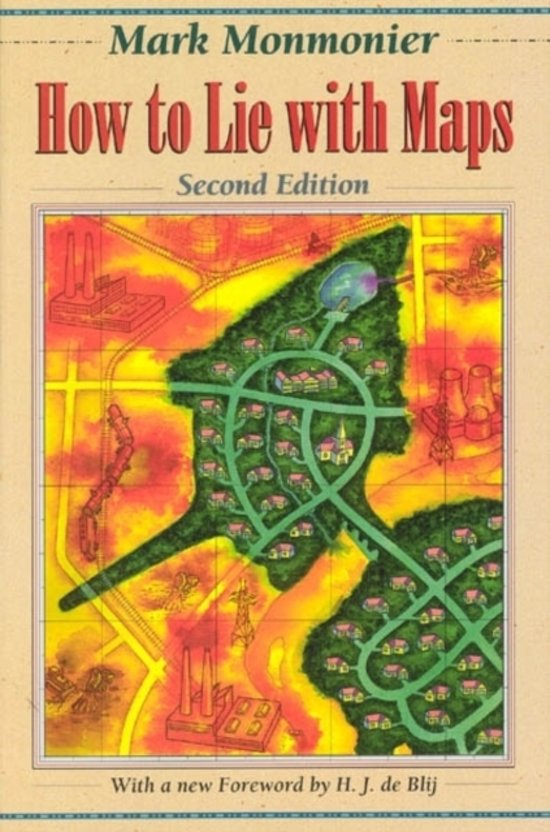
\includegraphics[width = 0.15\textwidth]{HowToLieWithMaps.jpg}
%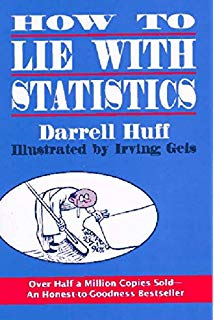
\includegraphics[width = 0.15\textwidth]{HowToLieWithStatistics.jpg}
%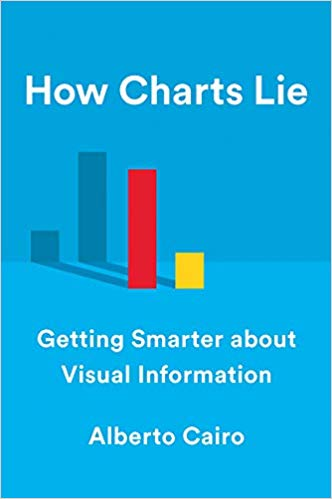
\includegraphics[width = 0.15\textwidth]{HowChartsLie.jpg}
%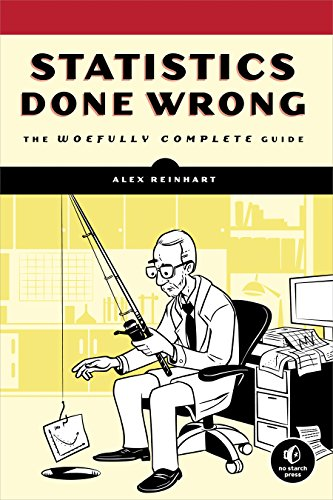
\includegraphics[width = 0.15\textwidth]{StatisticsDoneWrong.jpg}
%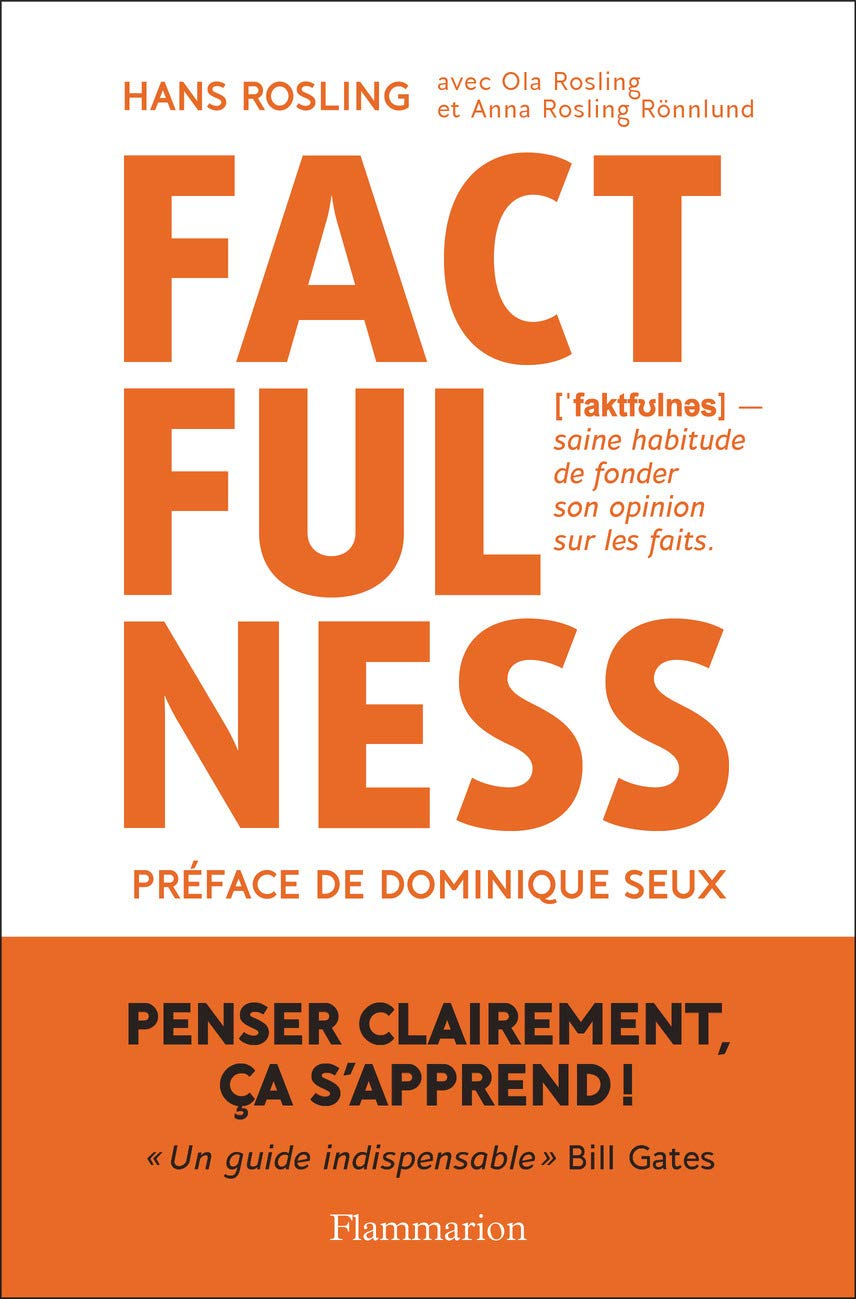
\includegraphics[width = 0.15\textwidth]{Factfulness.jpg}
%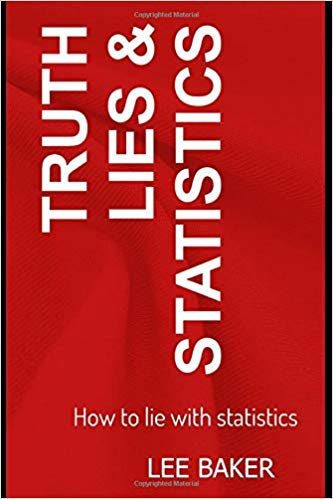
\includegraphics[width = 0.15\textwidth]{TruthLiesStatistics.jpg}
%\end{center}
%\end{frame}






\section{Lies}

\begin{frame} % Cover slide
\frametitle{\textcolor{brique}{[- \textbf{This lecture } -]}}

\begin{itemize}
  \item<+->[]\textcolor{brique}{Definition}:
   \item<+->[``\textbf{Lie}'']: What You See (on a graphic)\\ Is \textbf{Not} \\
                                What You Have (in the data)
  %\item<+->[]\textcolor{brique}{Observation:}\\ Many (conflicting) ``rules'' on dataviz
  \item<+->[]\textcolor{brique}{Goal:}\\ Help decipher graphics and identify visual lies
 % \item<+->[]\textcolor{brique}{Outcome:}\\ 10+ rules for ``lying'' in a future communication?
 % \item<+->[]At least, it is \textbf{fun}!
\end{itemize}
\end{frame}

\begin{frame} % Cover slide
\frametitle{\textcolor{brique}{Visual lies can be anywhere [Packaging!]}}
\begin{itemize}
  \item<+->[]
   \only<2> {
\includegraphics[width = 0.6\textwidth]{ChipsBags0.jpg}}
   \only<3> {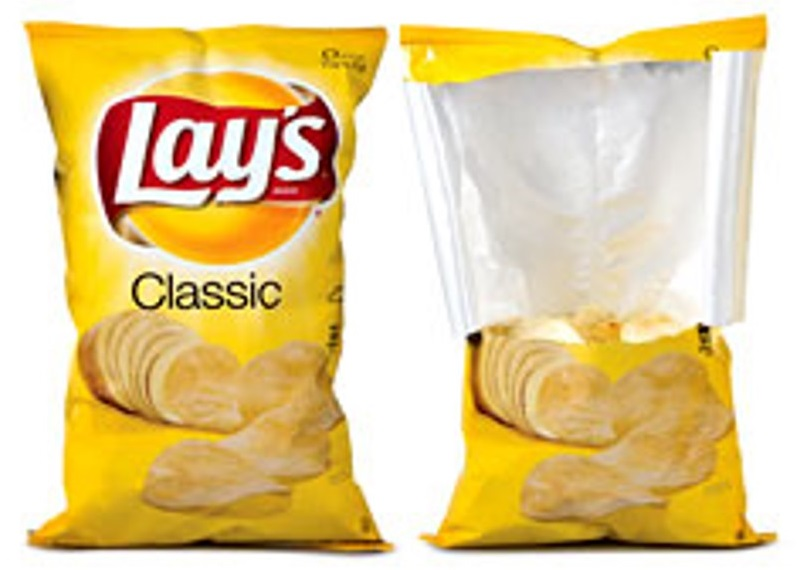
\includegraphics[width = 0.6\textwidth]{ChipsBags1.jpg}}
   \end{itemize}
\end{frame}



\begin{frame} % Cover slide
\frametitle{\textcolor{brique}{Visual lies can be anywhere [Pictures!]}}
\begin{itemize}
  \item<+->[]
   \only<2> {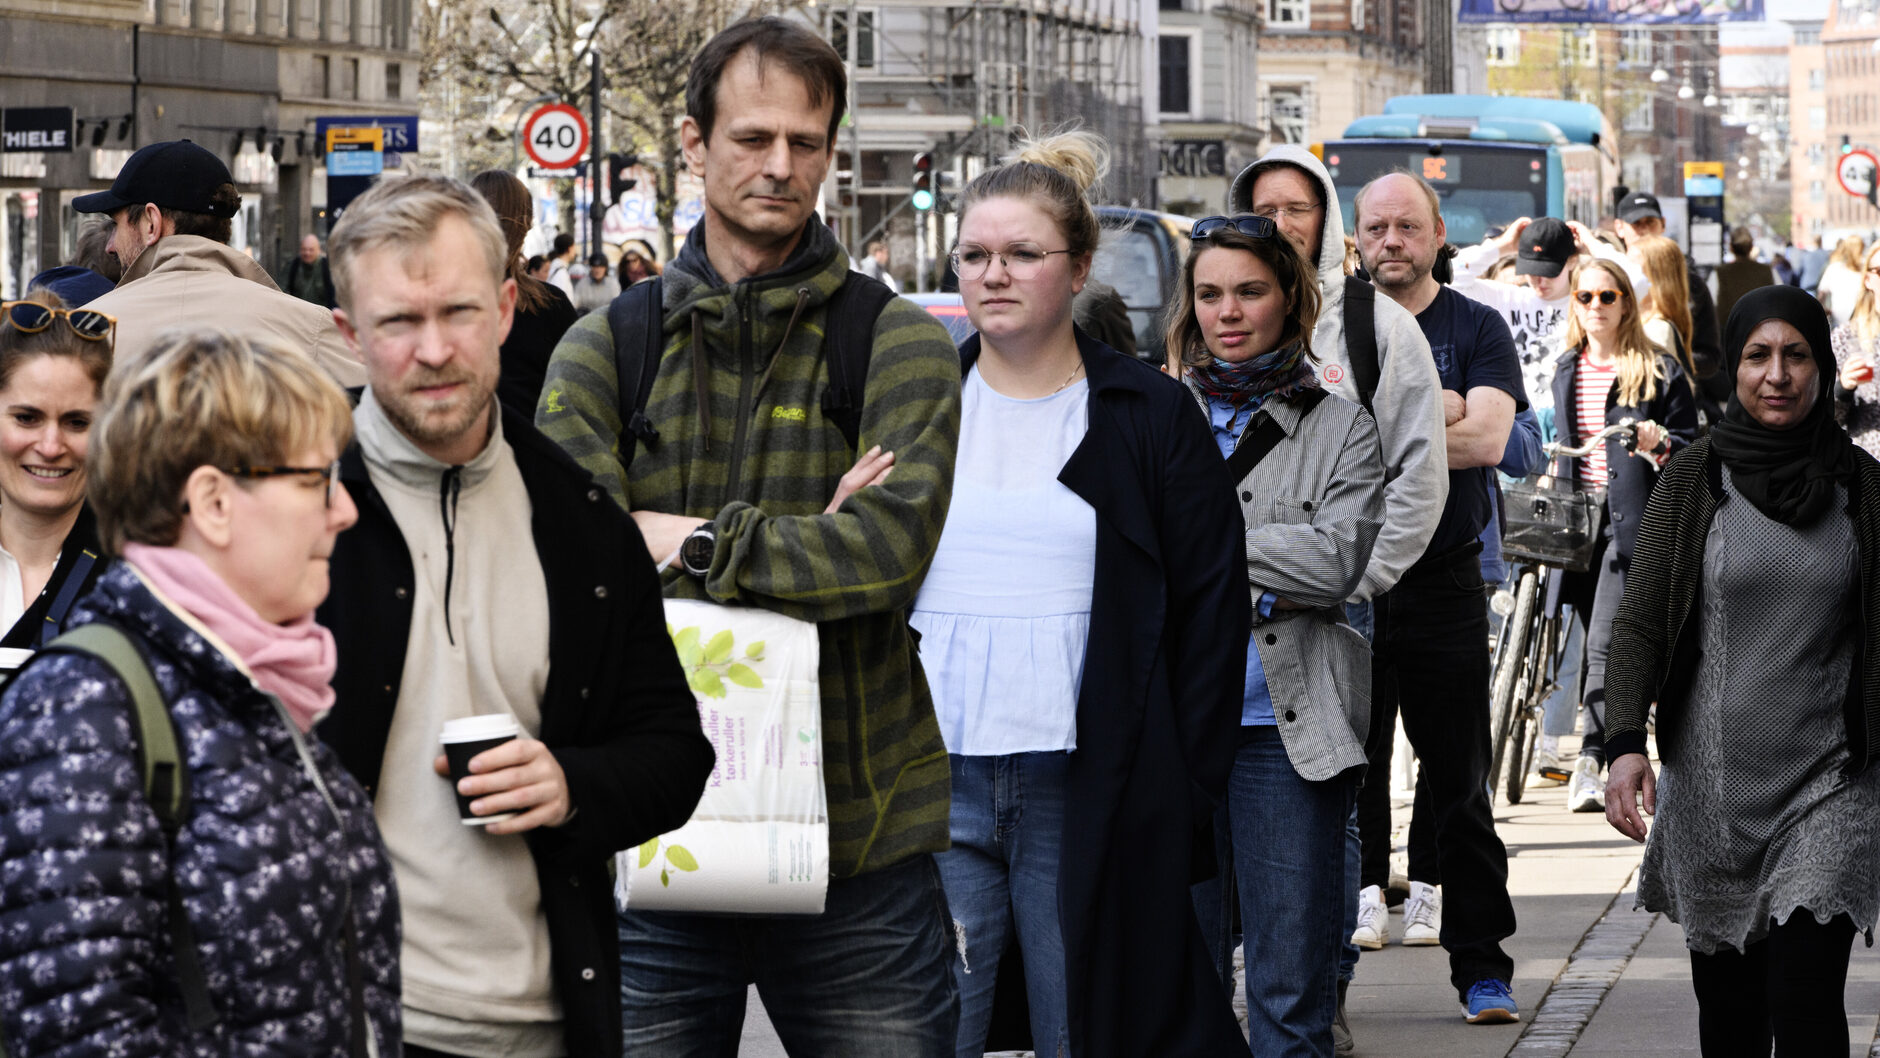
\includegraphics[width = 0.8\textwidth]{PhotoLineZoomed.jpg}\\ }
   \only<3> {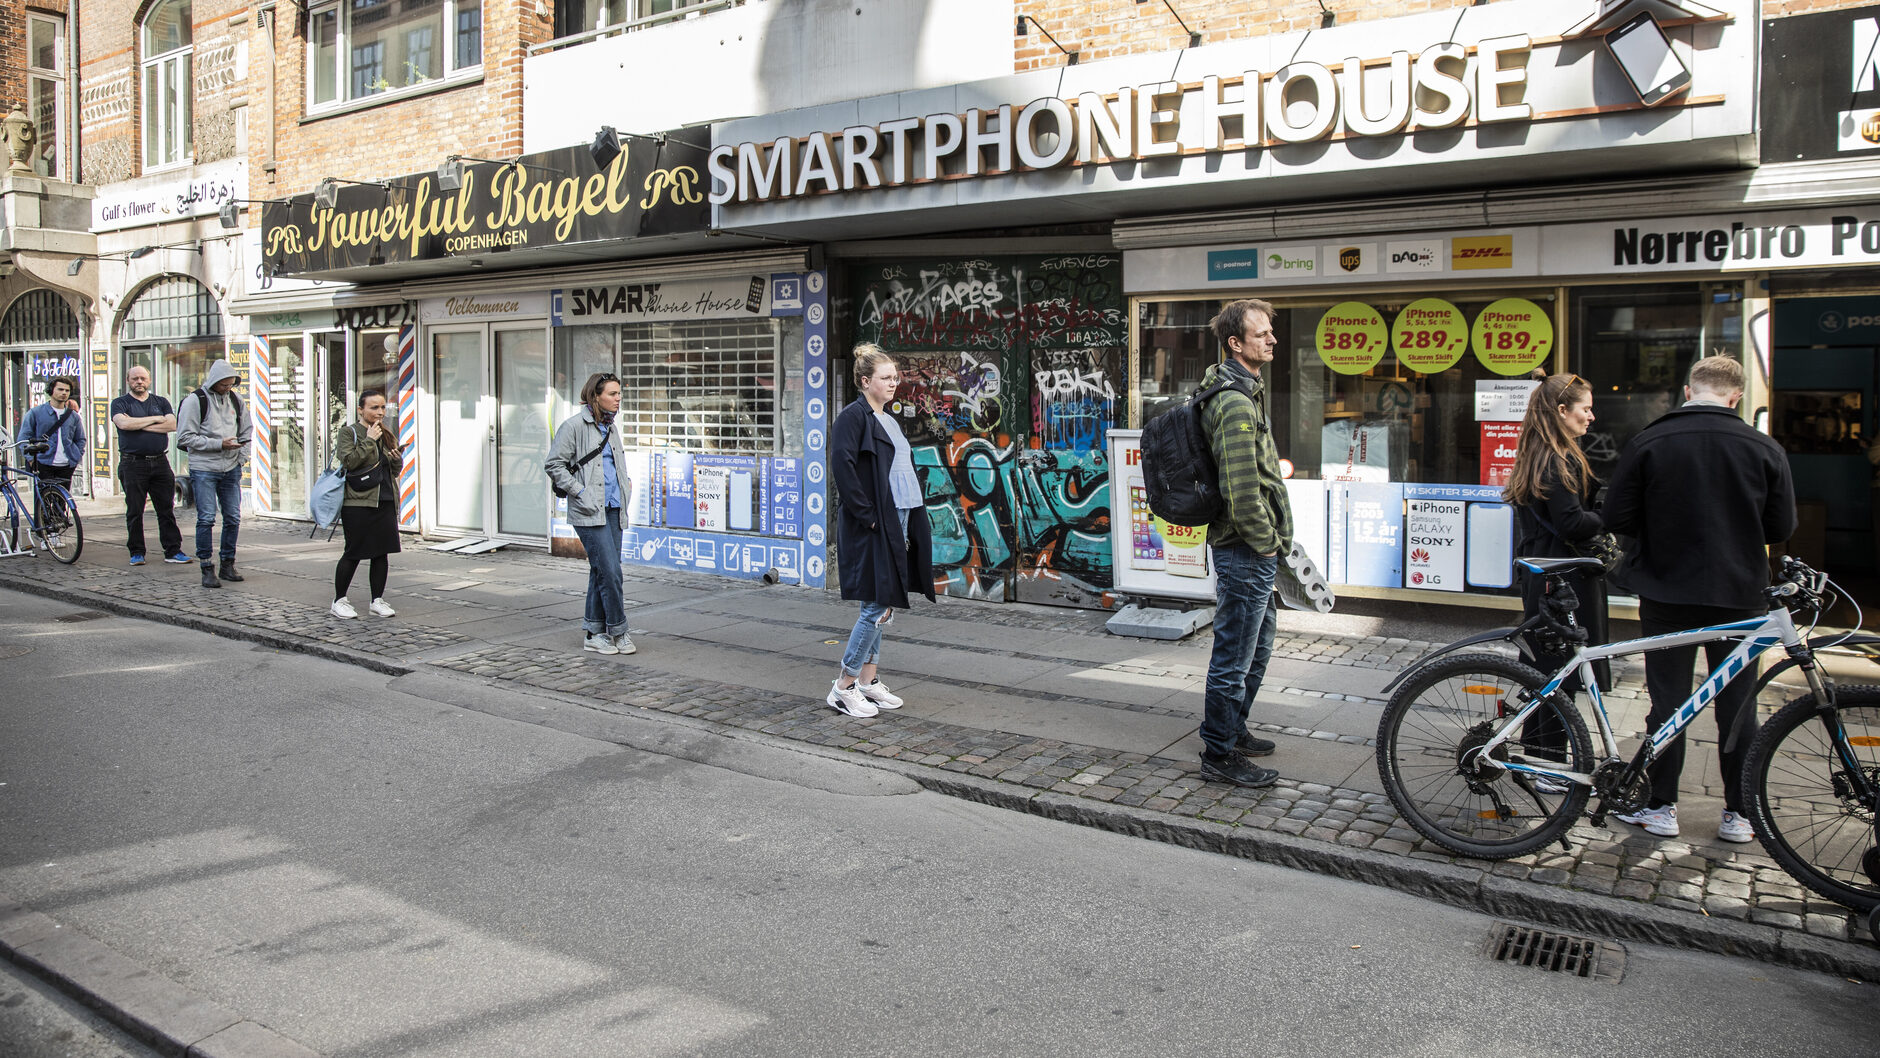
\includegraphics[width = 0.8\textwidth]{PhotoLineDeZoomed.jpg}\\ }
   \only<2-3>{\textcolor{gris}{\footnotesize{Source: \href{https://nyheder.tv2.dk/samfund/2020-04-26-hvor-taet-er-folk-paa-hinanden-disse-billeder-er-taget-samtidig-men-viser-to}{Astrid Helmer M{\o}rck}}}}
   \end{itemize}
\end{frame}

%
%\begin{frame} % Cover slide
%\frametitle{\textcolor{brique}{Visual lies can be anywhere}}
%\begin{itemize}
%  \item<+->[]
%  \only<2>{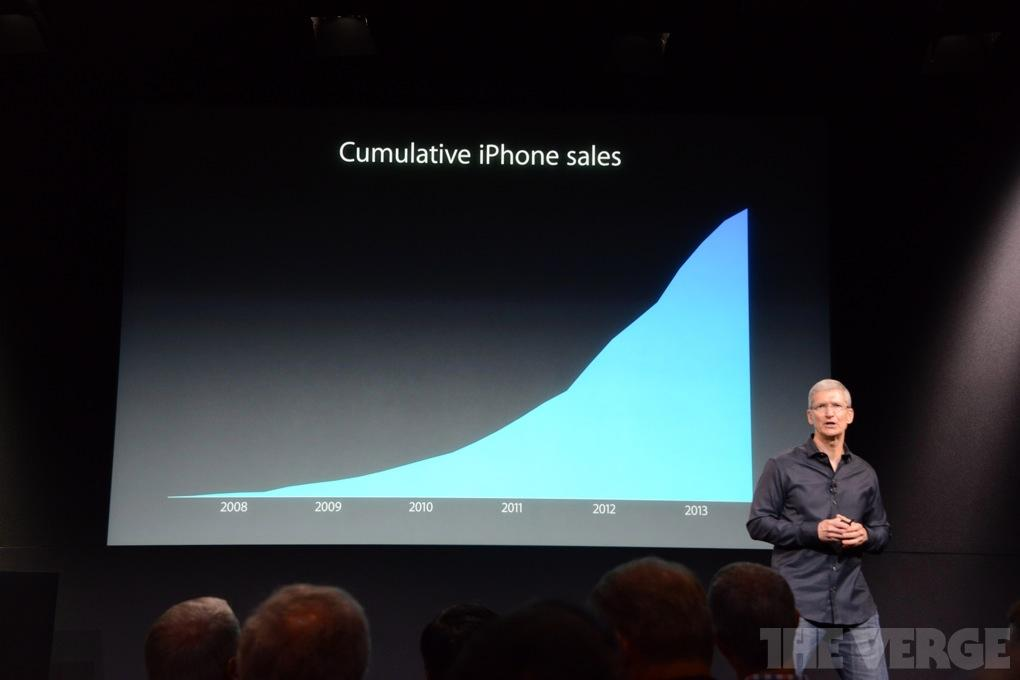
\includegraphics[width = 0.6\textwidth, height = 0.45\textwidth]{Cumulative-iphone-sales.jpg} \\ }
%  \only<3>{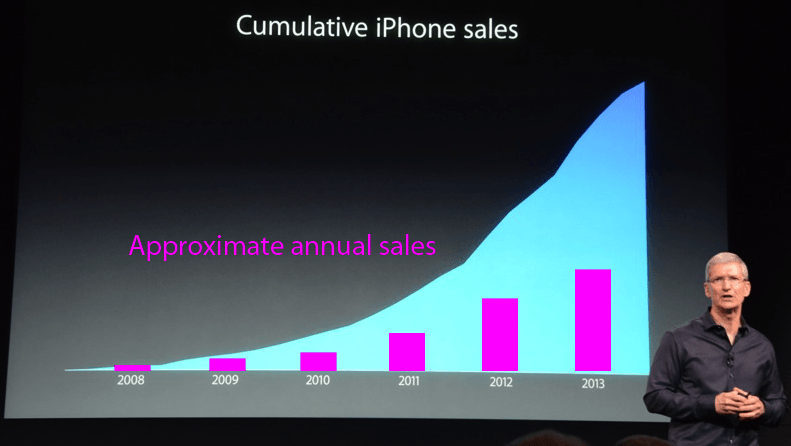
\includegraphics[width = 0.6\textwidth, height = 0.45\textwidth]{Cumulative-iphone-sales-rectified2.png}\\}
%  \only<2>{\textcolor{gris}{\footnotesize{Source: \href{https://qz.com/122921/the-chart-tim-cook-doesnt-want-you-to-see/}{David Yanofsky (Quartz)}}}}
%   \end{itemize}
%\end{frame}

\section{Rule 1}

\begin{frame} % Cover slide
\frametitle{\textcolor{brique}{[- \textbf{Rule \#1: Use devilish axis! } -]}}
\begin{center}
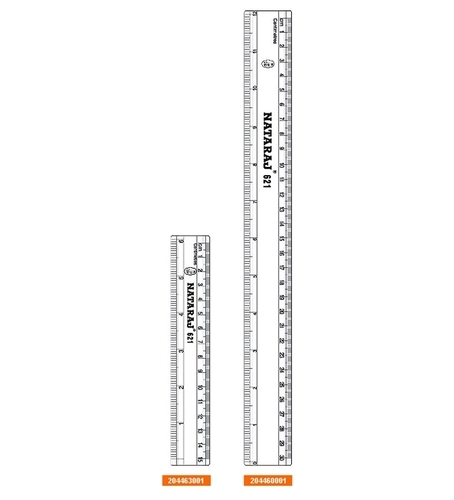
\includegraphics[width = 0.8\textwidth]{Scales.jpg}
\end{center}
\textcolor{gris}{\footnotesize{Source: https://www.dreamstime.com/}}
\end{frame}



\begin{frame} % Cover slide
\frametitle{\textcolor{brique}{[-\textbf{Rule \#1: Use devilish (truncated) axis! }-]}}
\begin{figure}
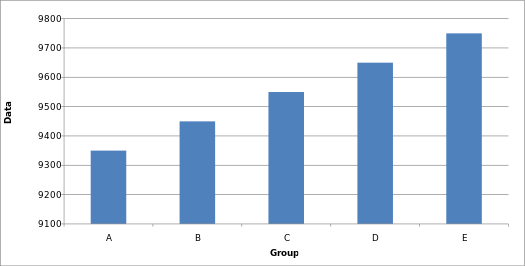
\includegraphics[width = 0.8\textwidth]{Truncated_Bar_Graph.png}
\end{figure}
\textcolor{gris}{\footnotesize{Source: \href{https://en.wikipedia.org/wiki/Misleading_graph}{Wikipedia: Misleading graph}}}  \hfill \textcolor{brique}{\textbf{Poll}}
\end{frame}

\begin{frame} % Cover slide
\frametitle{\textcolor{brique}{[-\textbf{Rule \#1: Use devilish (truncated) axis!}-]}}
\begin{figure}[h]
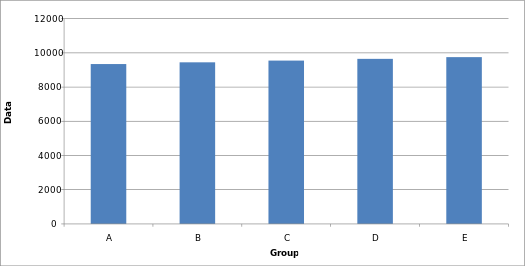
\includegraphics[width = 0.8\textwidth]{Bar_graph.png}
\end{figure}
\textcolor{gris}{\footnotesize{Source: \href{https://en.wikipedia.org/wiki/Misleading_graph}{Wikipedia: Misleading graph}}}

\end{frame}



\begin{frame} % Cover slide
\frametitle{\textcolor{brique}{[-\textbf{Rule \#1: Use devilish  axis!}-]}}
\begin{center}
\begin{itemize}
  \only<1>{ 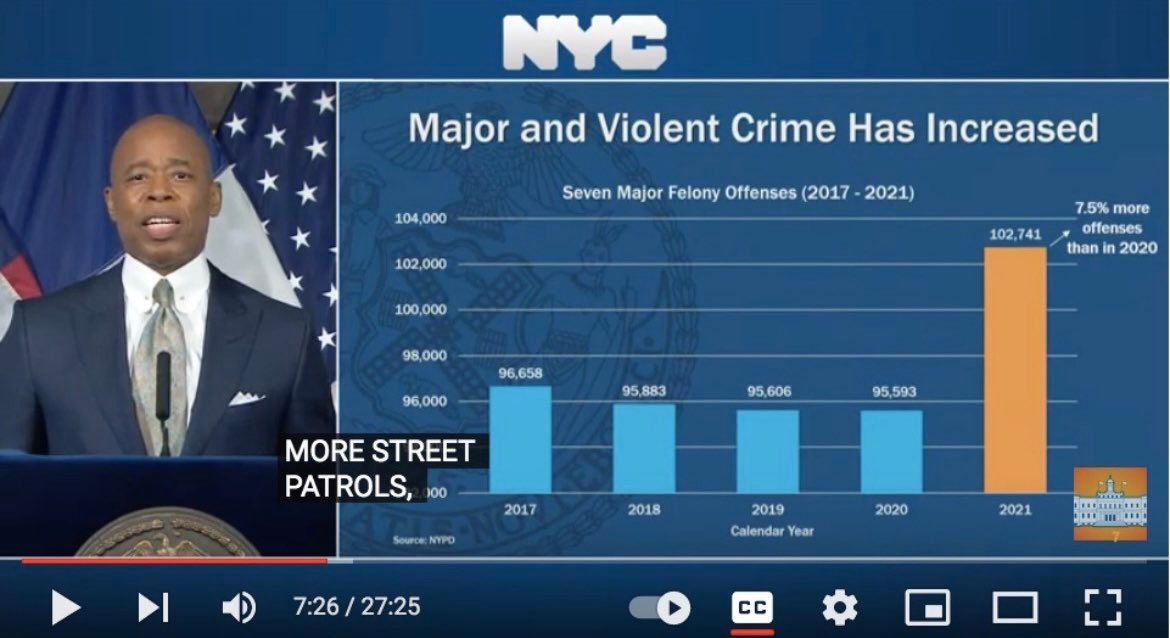
\includegraphics[width = 0.8\textwidth]{BarsNYC.jpeg} \\ }
  \only<2>{ 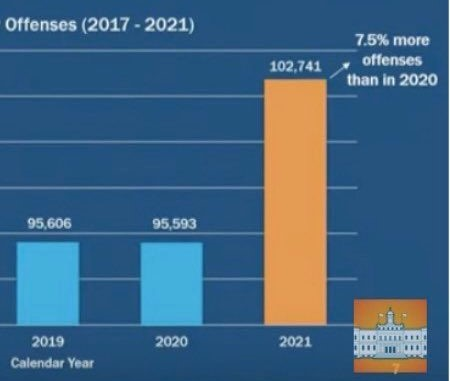
\includegraphics[width = 0.6\textwidth]{BarsNYC-zoom.jpeg} \\ }
  \only<3>{ \textbf{Initial} version \\ }
  \only<3>{ 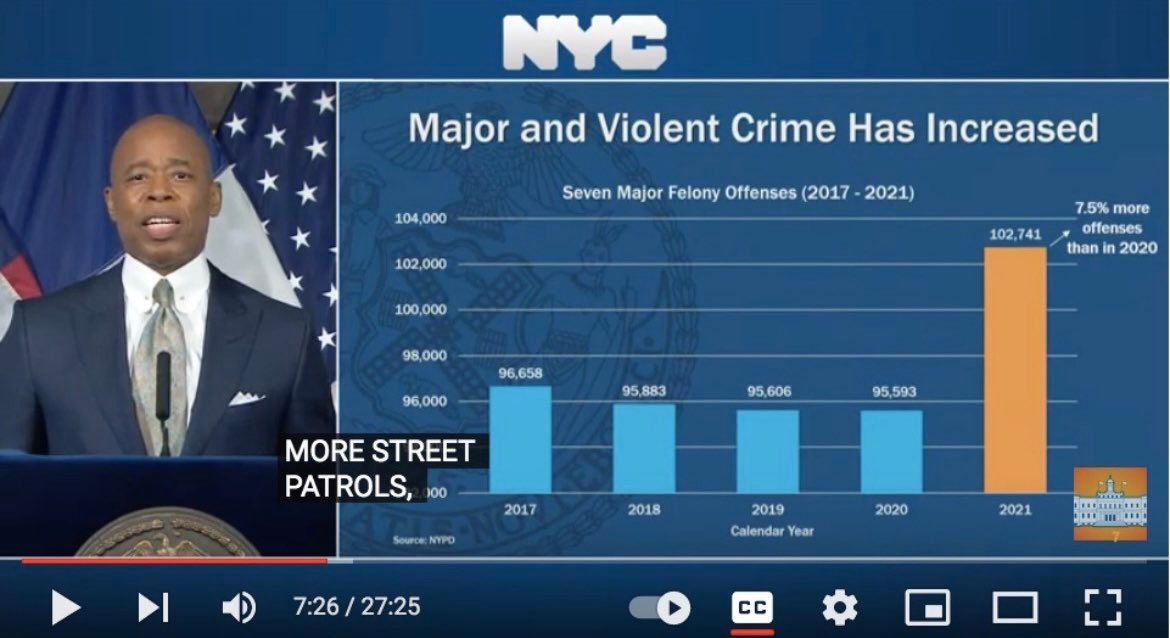
\includegraphics[width = 0.8\textwidth]{BarsNYC.jpeg} \\ }
  \only<4>{ \textbf{Correct} version \\ }
  \only<4>{ 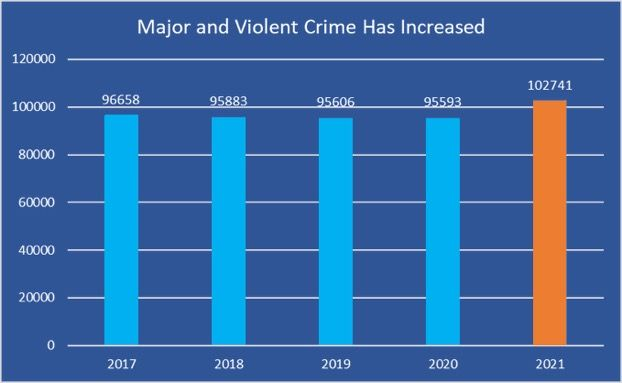
\includegraphics[width = 0.7\textwidth]{BarsNYC-Corrected.jpeg} \\ }
  \only<1-4>{\textcolor{gris}{\footnotesize{Source: \href{https://twitter.com/bradlander/status/1494066688110833665?s=21}{Brad Lander (twitter) - New York City Mayor Eric Adams}}}}
%  \only<5>{ \textbf{In context} version (see  also \textbf{Rule \#4} )\\ }
%  \only<5>{ 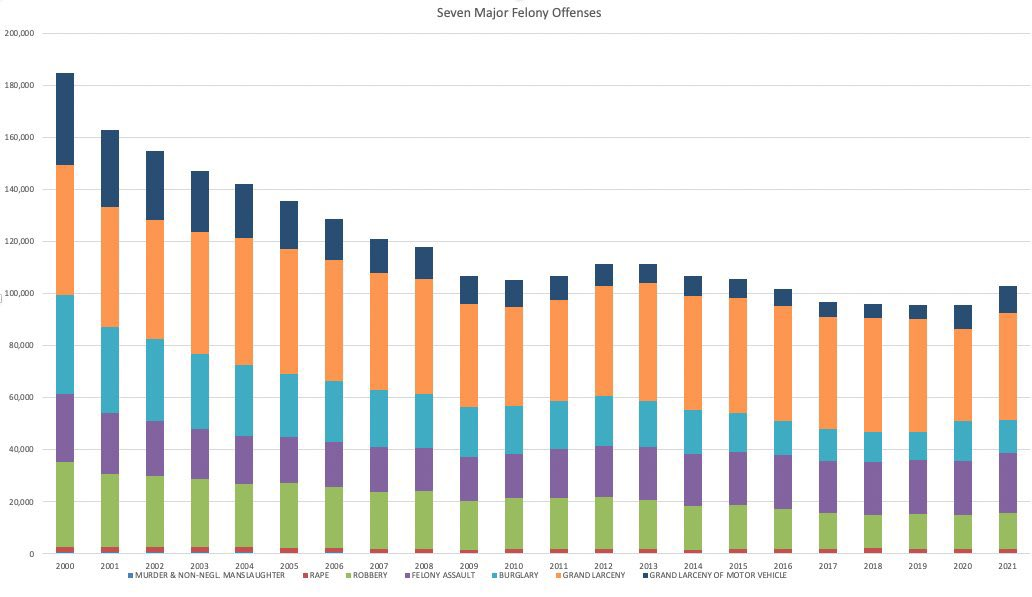
\includegraphics[width = 0.8\textwidth]{BarsNYC-long.jpeg} \\ }
%  \only<5>{\textcolor{gris}{\footnotesize{Source: \href{https://twitter.com/bradlander/status/1494093635092197381}{Cooper Lund (twitter)}}}}
\end{itemize}
\end{center}
\end{frame}


%\begin{frame} % Cover slide
%\frametitle{\textcolor{brique}{[-\textbf{Rule \#1-bis: Use truncated X-axis!}-]}}
%
%\begin{center}
%\begin{itemize}
%\only<1>{\textbf{Examples} are common! \\ }
%  \only<1>{ 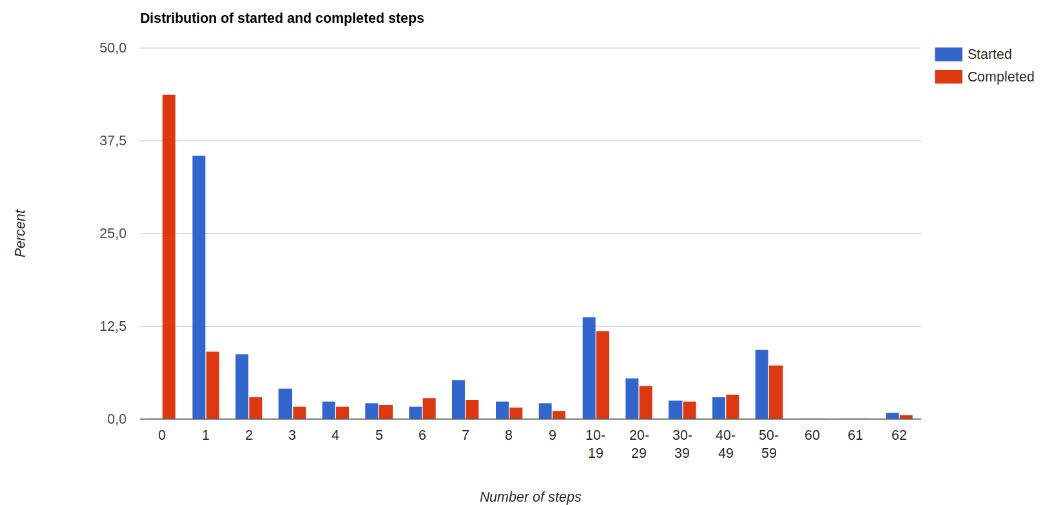
\includegraphics[width = 0.9\textwidth]{Mistake-barchart.jpg} \\ }
%  \only<1>{\textcolor{gris}{\footnotesize{Source: My 2017' students (Jan \& Mohamed)}} \hfill \textcolor{brique}{\textbf{Poll}}  }
%  \only<2>{\textbf{Examples} are common! \\ }
%  \only<2>{ 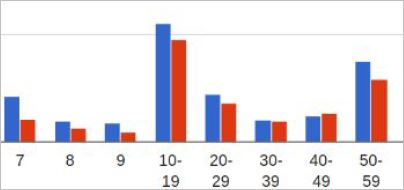
\includegraphics[width = 0.7\textwidth]{XAxisScaleChange.JPG} \\  }
%  \only<2>{\textcolor{gris}{\footnotesize{Source: My 2017' students (Jan \& Mohamed)}}   }
%  \only<3>{\textbf{Published example} are common! \\ }
%%  \only<3>{ 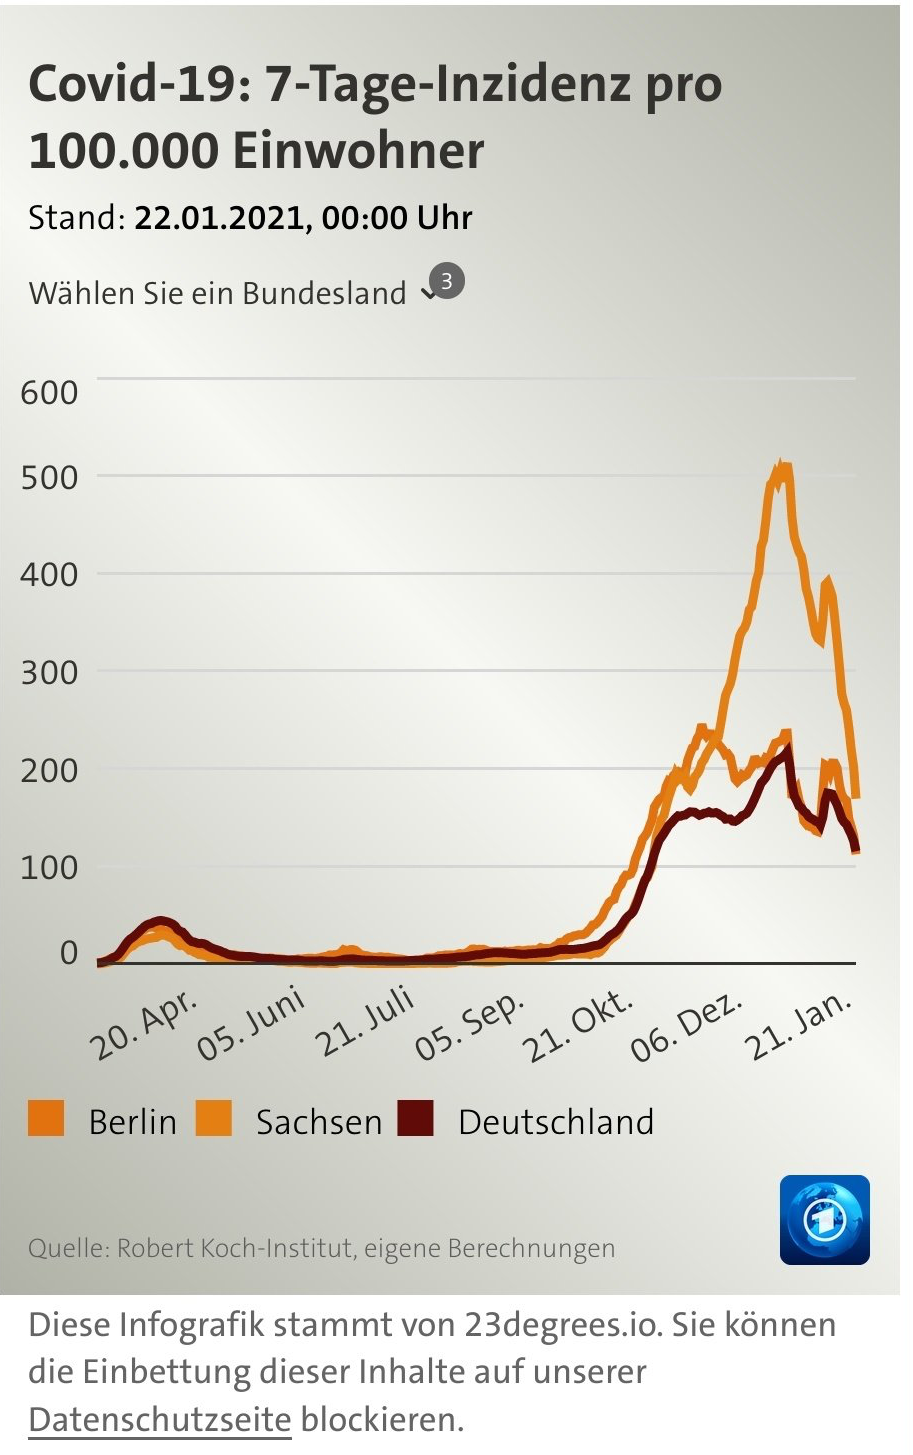
\includegraphics[width = 0.5\textwidth]{Lie-X-Axis-Covid.png}}
%%  \only<4>{ 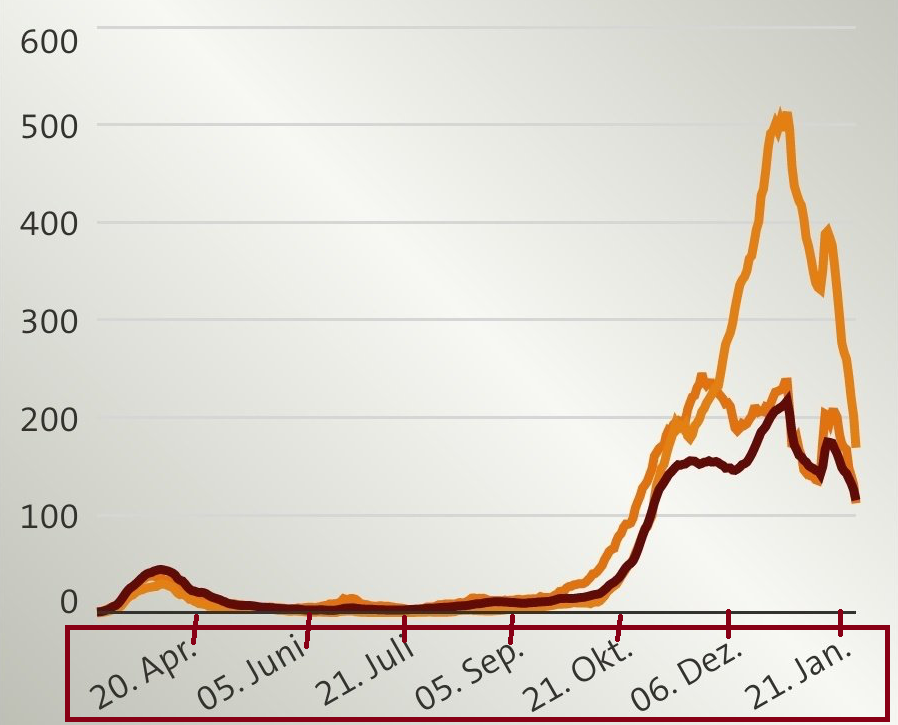
\includegraphics[width = 0.7\textwidth]{Lie-X-Axis-Covid-Zoom.png}}
% \only<3>{ 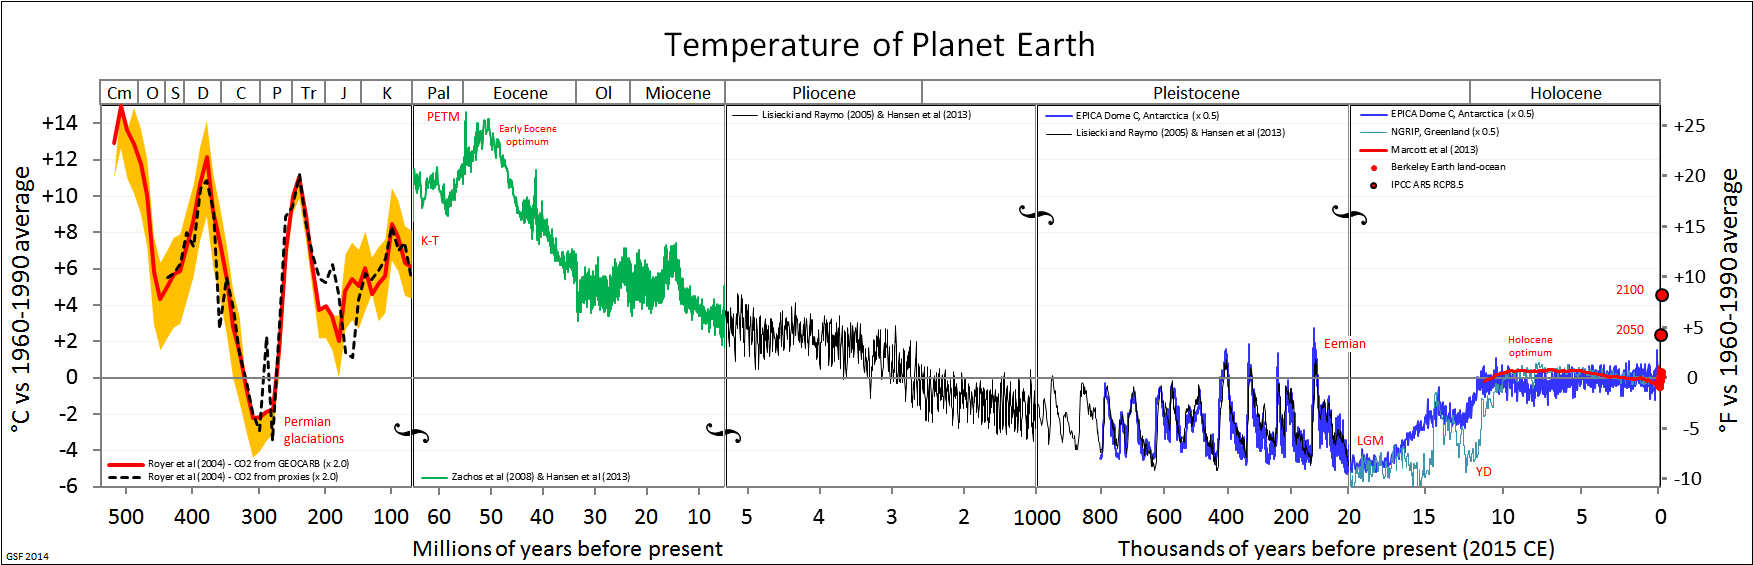
\includegraphics[width = 0.9\textwidth]{ Axe_palaeotemps.png}}
% \only<3>{\textcolor{gris}{\footnotesize{Source: \href{https://en.wikipedia.org/wiki/Talk:Geologic_temperature_record}{Wikipedia}}}}
%\end{itemize}
%\end{center}
%\end{frame}

%
%\begin{frame} % Cover slide
%\frametitle{\textcolor{brique}{[-\textbf{Entering complexity }-]}}
%Example: Fox news
%\begin{figure}[h]
%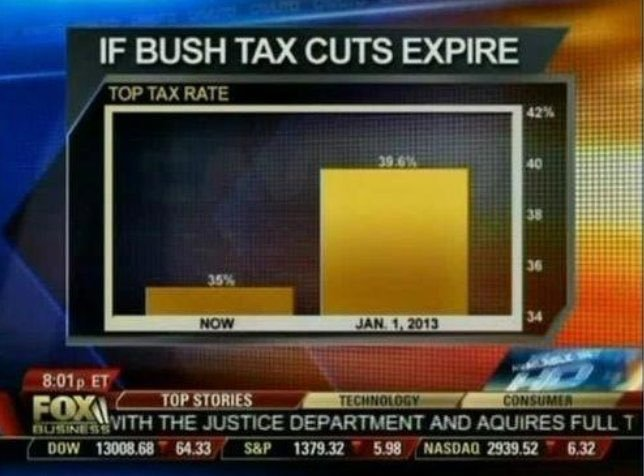
\includegraphics[width = 0.8\textwidth]{BarChartFoxBush.jpg}
%\end{figure}
%\textcolor{gris}{\footnotesize{Source: \href{https://technaverbascripta.wordpress.com/2014/04/16/lying-with-data-visualizations-is-it-misleading-to-truncate-the-y-axis/}{Techna Verba Scripta}}}
%\end{frame}
%
%
%\begin{frame} % Cover slide
%\frametitle{\textcolor{brique}{[-\textbf{Entering complexity}-]}}
%
%\begin{center}
%\begin{itemize}
%  \only<1>{So this is bad:\\ }
%  \only<1>{ 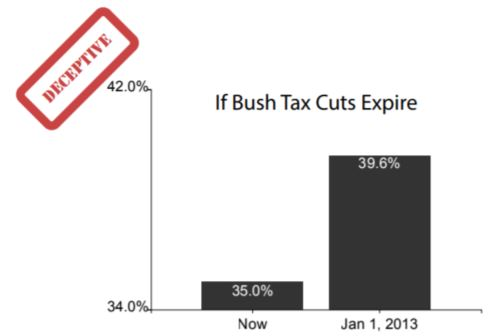
\includegraphics[width = 0.7\textwidth]{TruncatingAxis-BarsBad-Correll2019.JPG}}
%  \only<2>{This is good: \\}
%  \only<2>{ 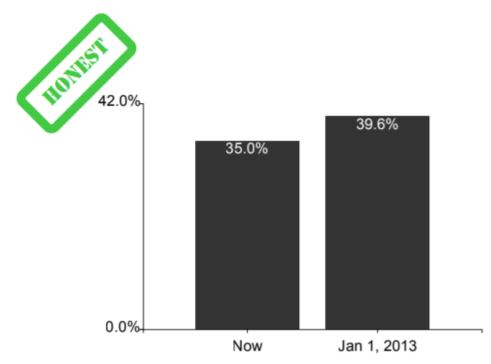
\includegraphics[width = 0.7\textwidth]{TruncatingAxis-BarsGood-Correll2019.JPG}}
%  \only<3>{This is also bad:\\ }
%  \only<3>{ 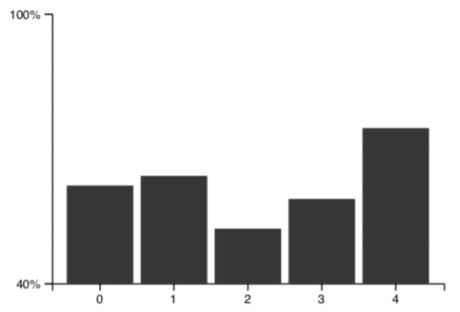
\includegraphics[width = 0.8\textwidth]{ExperienceTruncatingAxis-Bars-Correll2019.JPG}}
%  \only<4>{Bad or good? \\ }
%  \only<4>{ 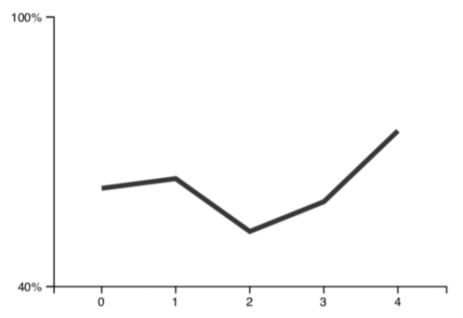
\includegraphics[width = 0.8\textwidth]{ExperienceTruncatingAxis-Lines-Correll2019.JPG}}
%  \only<5>{\cite{Correll2019} show empirically that there is: \\
%   `` \textit{no robust difference (...):  truncation serves to exaggerate effect sizes in \textbf{both} types of graphs.''}\\
% 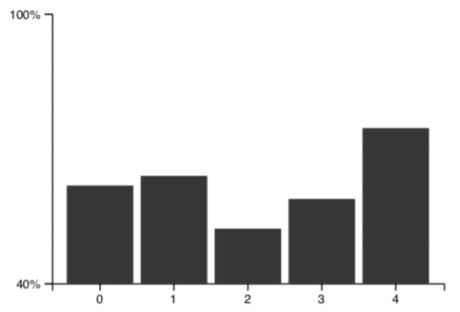
\includegraphics[width = 0.4\textwidth]{ExperienceTruncatingAxis-Bars-Correll2019.JPG} 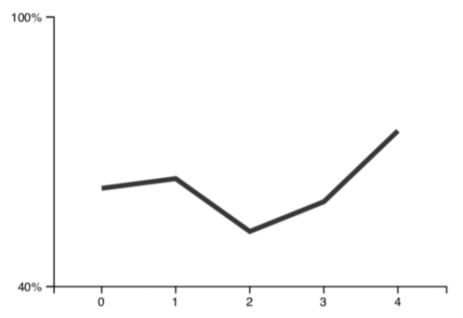
\includegraphics[width = 0.4\textwidth]{ExperienceTruncatingAxis-Lines-Correll2019.JPG}}
%  \only<6>{Bad? \\ }
%  \only<6>{ 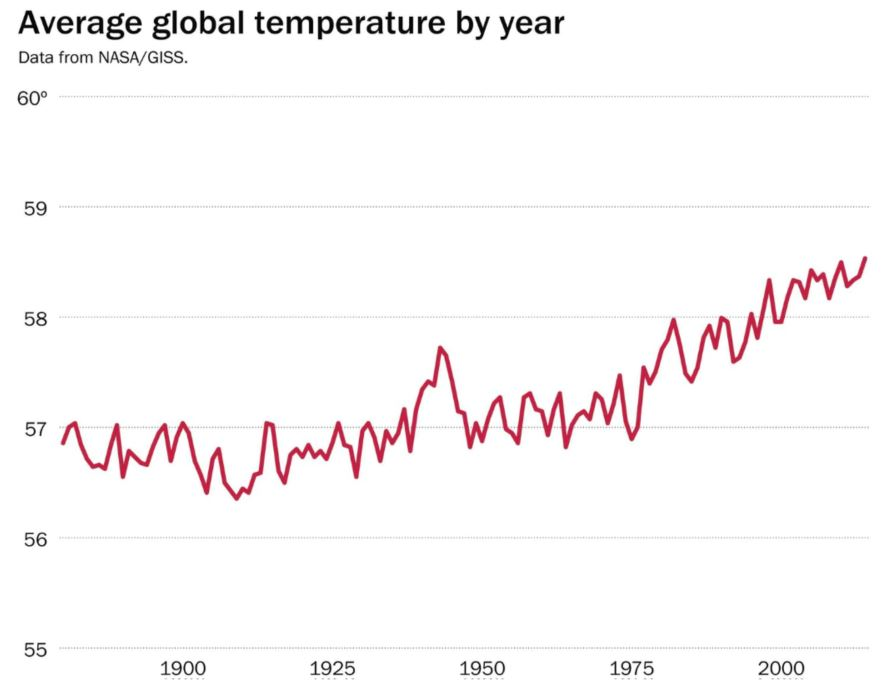
\includegraphics[width = 0.75\textwidth]{AverageGlobalTemperature-Truncated.JPG}\\ }
%  \only<6>{\textcolor{gris}{\footnotesize{\href{https://en.wikipedia.org/wiki/Misleading_graph}{Washington Post (December, 2015)}}}}
%  \only<7>{Good? \\ }
%  \only<7>{ 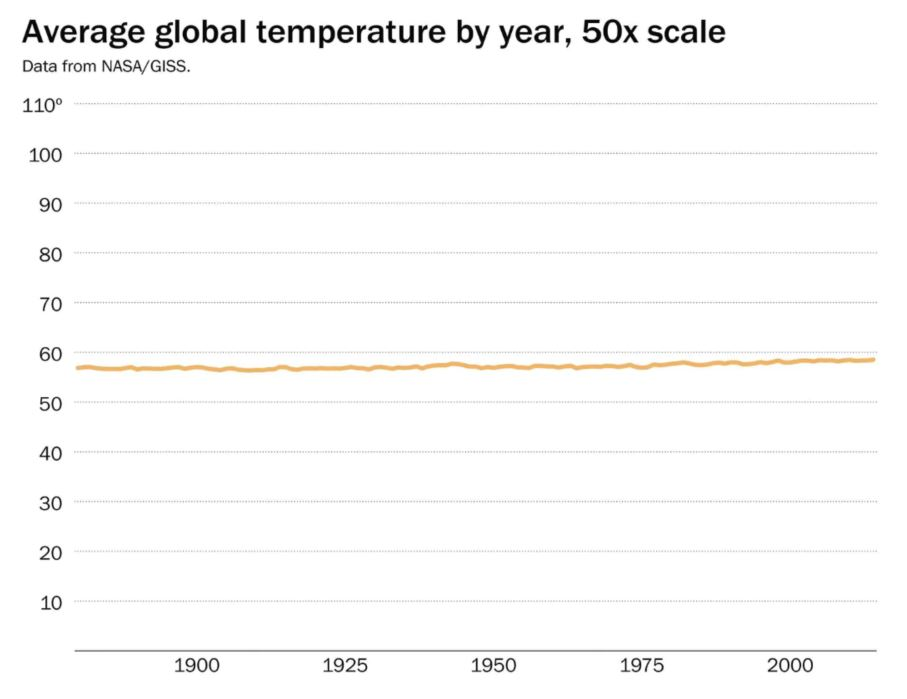
\includegraphics[width = 0.8\textwidth]{AverageGlobalTemperature-Misleading.JPG}\\ }
%  \only<7>{\textcolor{gris}{\footnotesize{\href{https://en.wikipedia.org/wiki/Misleading_graph}{Washington Post, reproducing National Review  (December, 2015)}}}}
%\end{itemize}
%\end{center}
%\end{frame}

%\begin{frame} % Cover slide
%\frametitle{\textcolor{brique}{[-\textbf{How (not) to be misleading?}-]}}
%\begin{center}
%\begin{itemize}
%  \only<1> {\textcolor{brique}{\textbf{Ruling}} is hard! \\ }
%  \only<1>{ 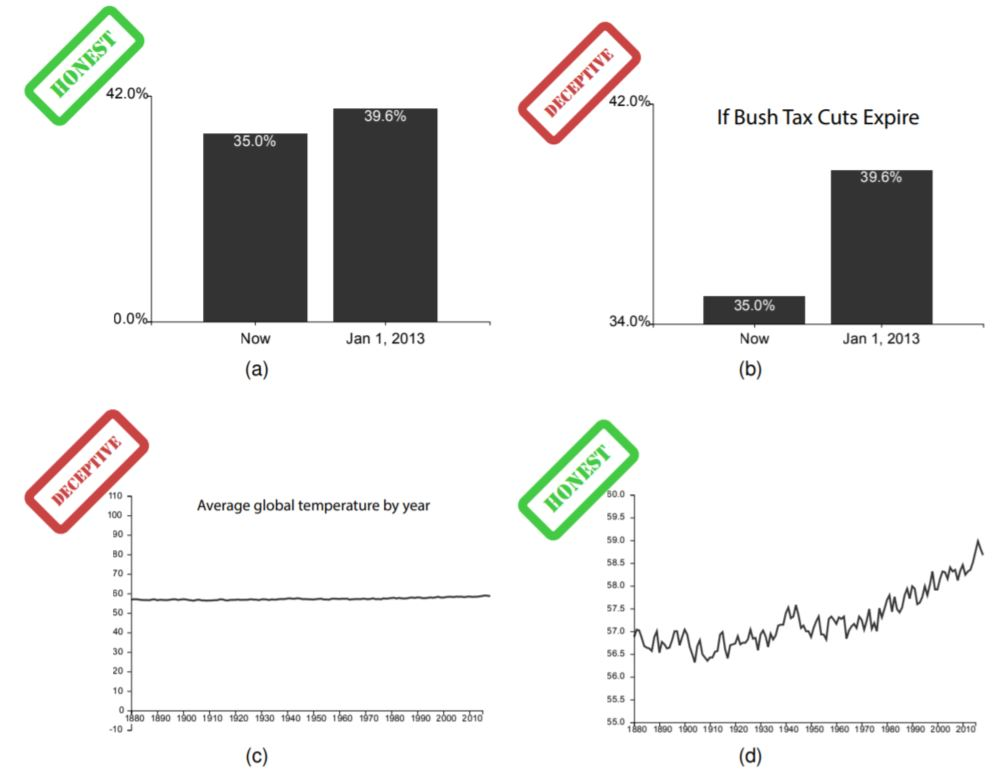
\includegraphics[width = 0.8\textwidth]{TruncatingAxis-All-Correll2019.JPG}}
%  \only<2>{\textbf{Discussed} by many: \\ }
%  \only<2> {\cite{Cairo2019}, \\ \cite{Correll2019}, \\ \cite{Allen2016}, \\
%            \cite{Isenberg2011}, \\ \cite{Kelleher2011}, \\
%            \cite{Tufte2001}, \\
%            \cite{Cleveland1982} \\
%             $\cdots$ \\ }
%  \only<3> {So \textcolor{brique}{\textbf{lying}} is easy :\\ }
%  \only<3> {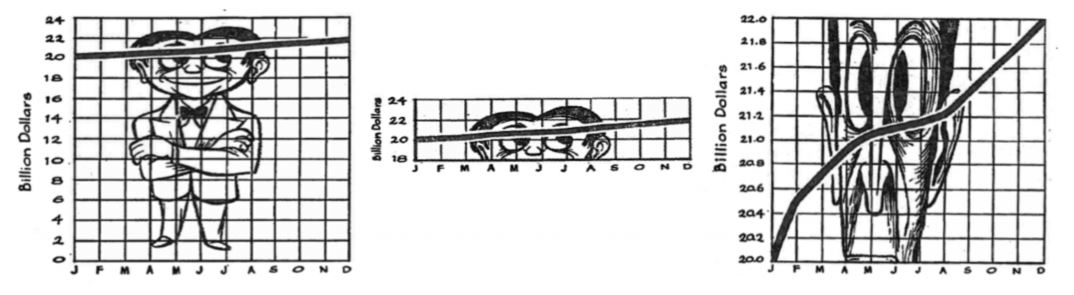
\includegraphics[width = 1.0\textwidth]{MisleadingScales-Duff.JPG} \\}
%  \only<3> {From \cite{Huff1993}}
%\end{itemize}
%\end{center}
%\end{frame}
\section{Rule 2}

\begin{frame}
\frametitle{\textcolor{brique}{[-\textbf{Rule \#2: Play with scales!}-]}}
\begin{center}
\begin{itemize}
  \only<1>{Here is a graphic }
  \only<1>{ 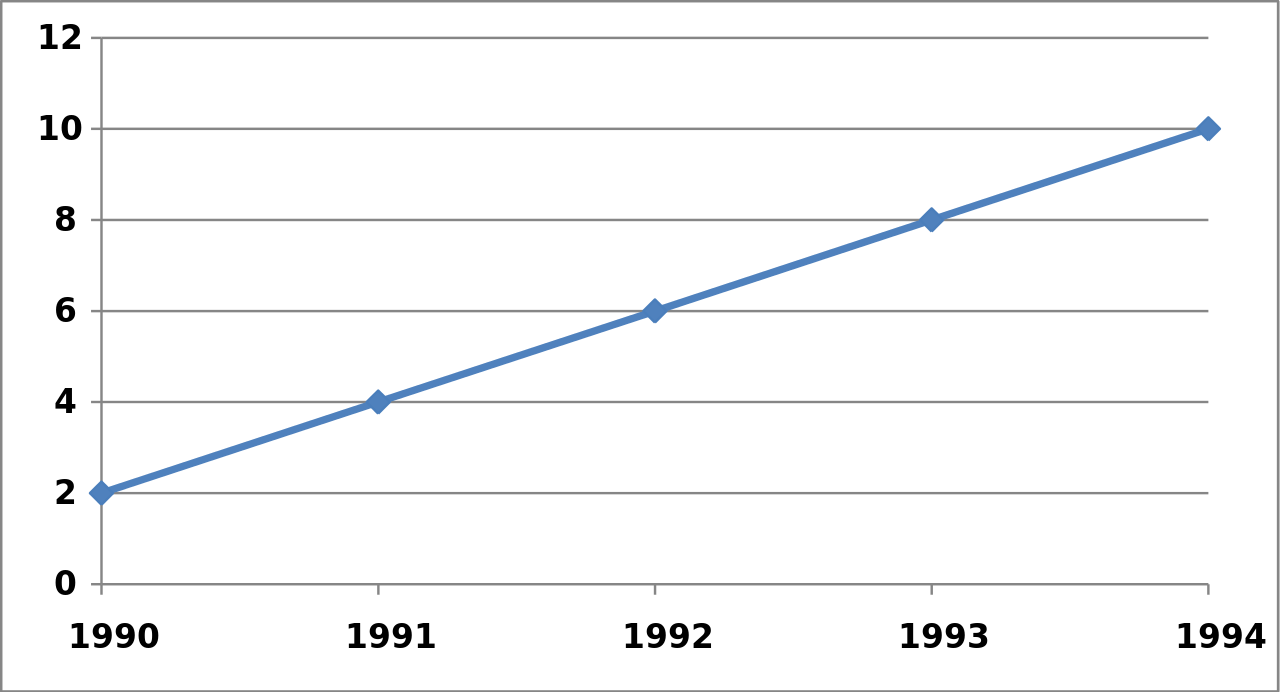
\includegraphics[width = 0.8\textwidth]{Line_graph1.png}}
  \only<2>{The same with a different \textbf{Y}-axis... }
  \only<2>{ 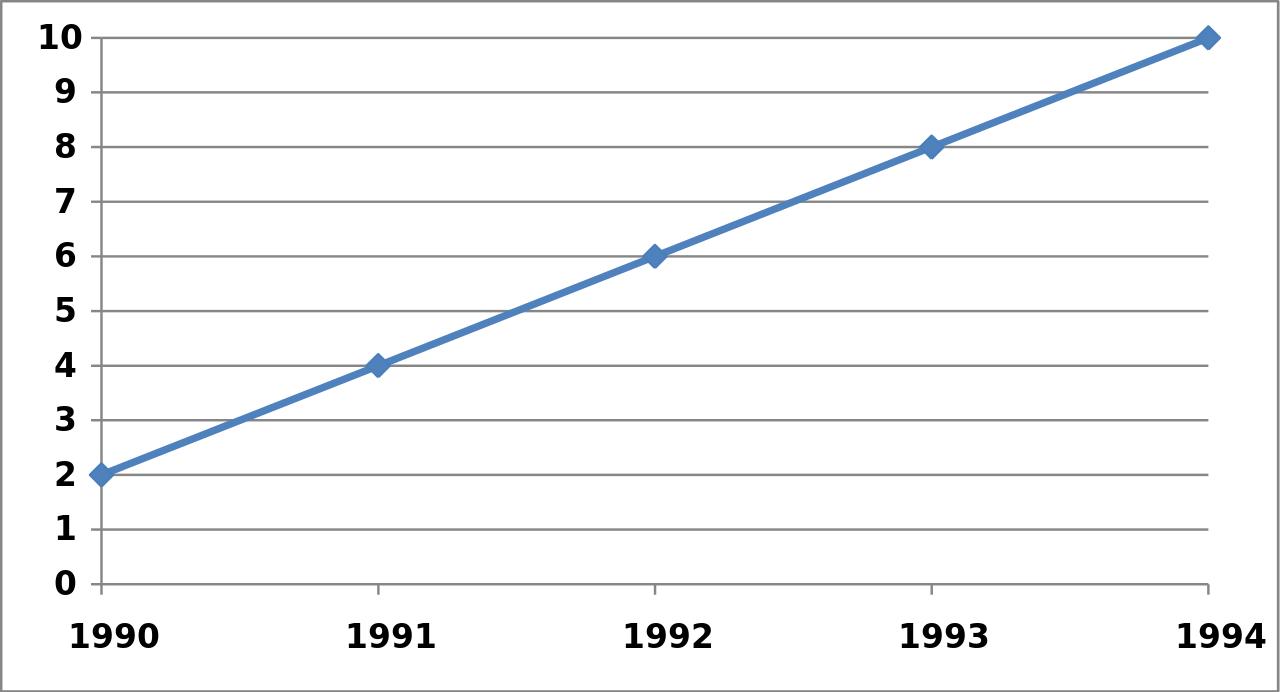
\includegraphics[width = 0.8\textwidth]{Line_graph3.png}}
  \only<3>{The same with a \textbf{Y}-axis that goes way beyond max(Y)... }
  \only<3>{ 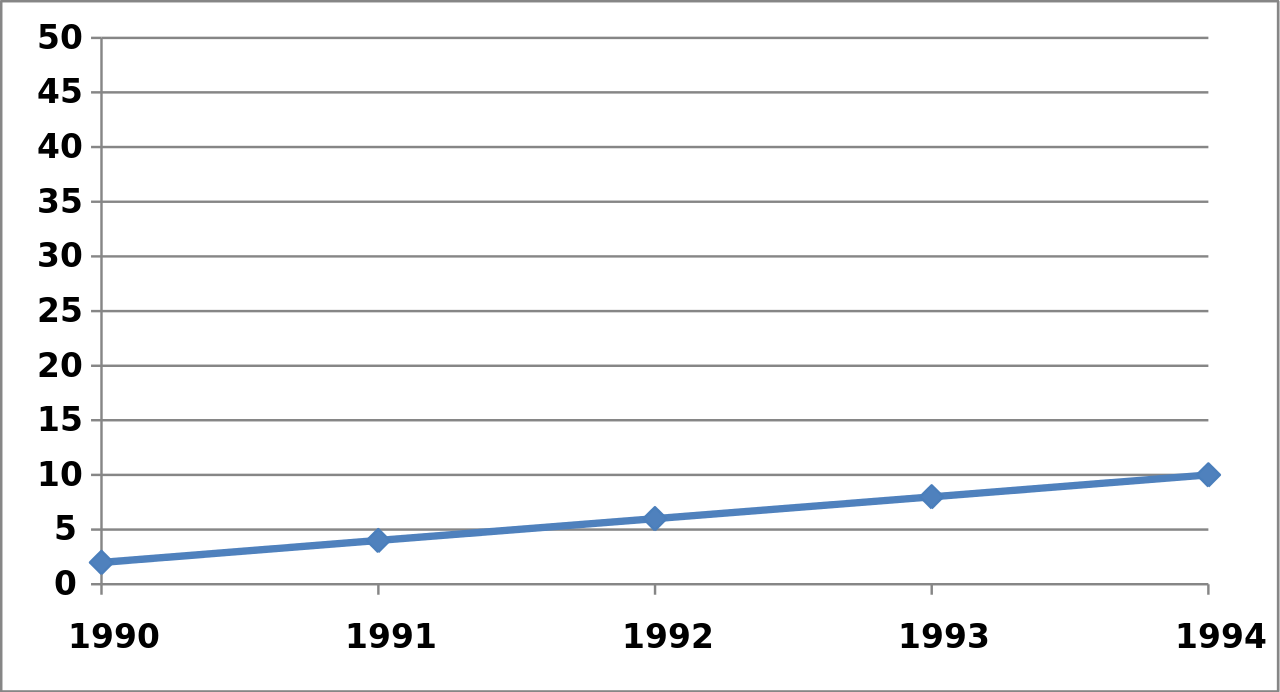
\includegraphics[width = 0.8\textwidth]{Line_graph2.png}}
\end{itemize}
\end{center}
\textcolor{gris}{\footnotesize{Source: \href{https://en.wikipedia.org/wiki/Misleading_graph}{Wikipedia: Misleading graph}}}
\end{frame}

\begin{frame} % Cover slide
\frametitle{\textcolor{brique}{[-\textbf{Rule \#2: Play with scales!}-]}}
\begin{center}
\begin{itemize}
  \only<1>{ 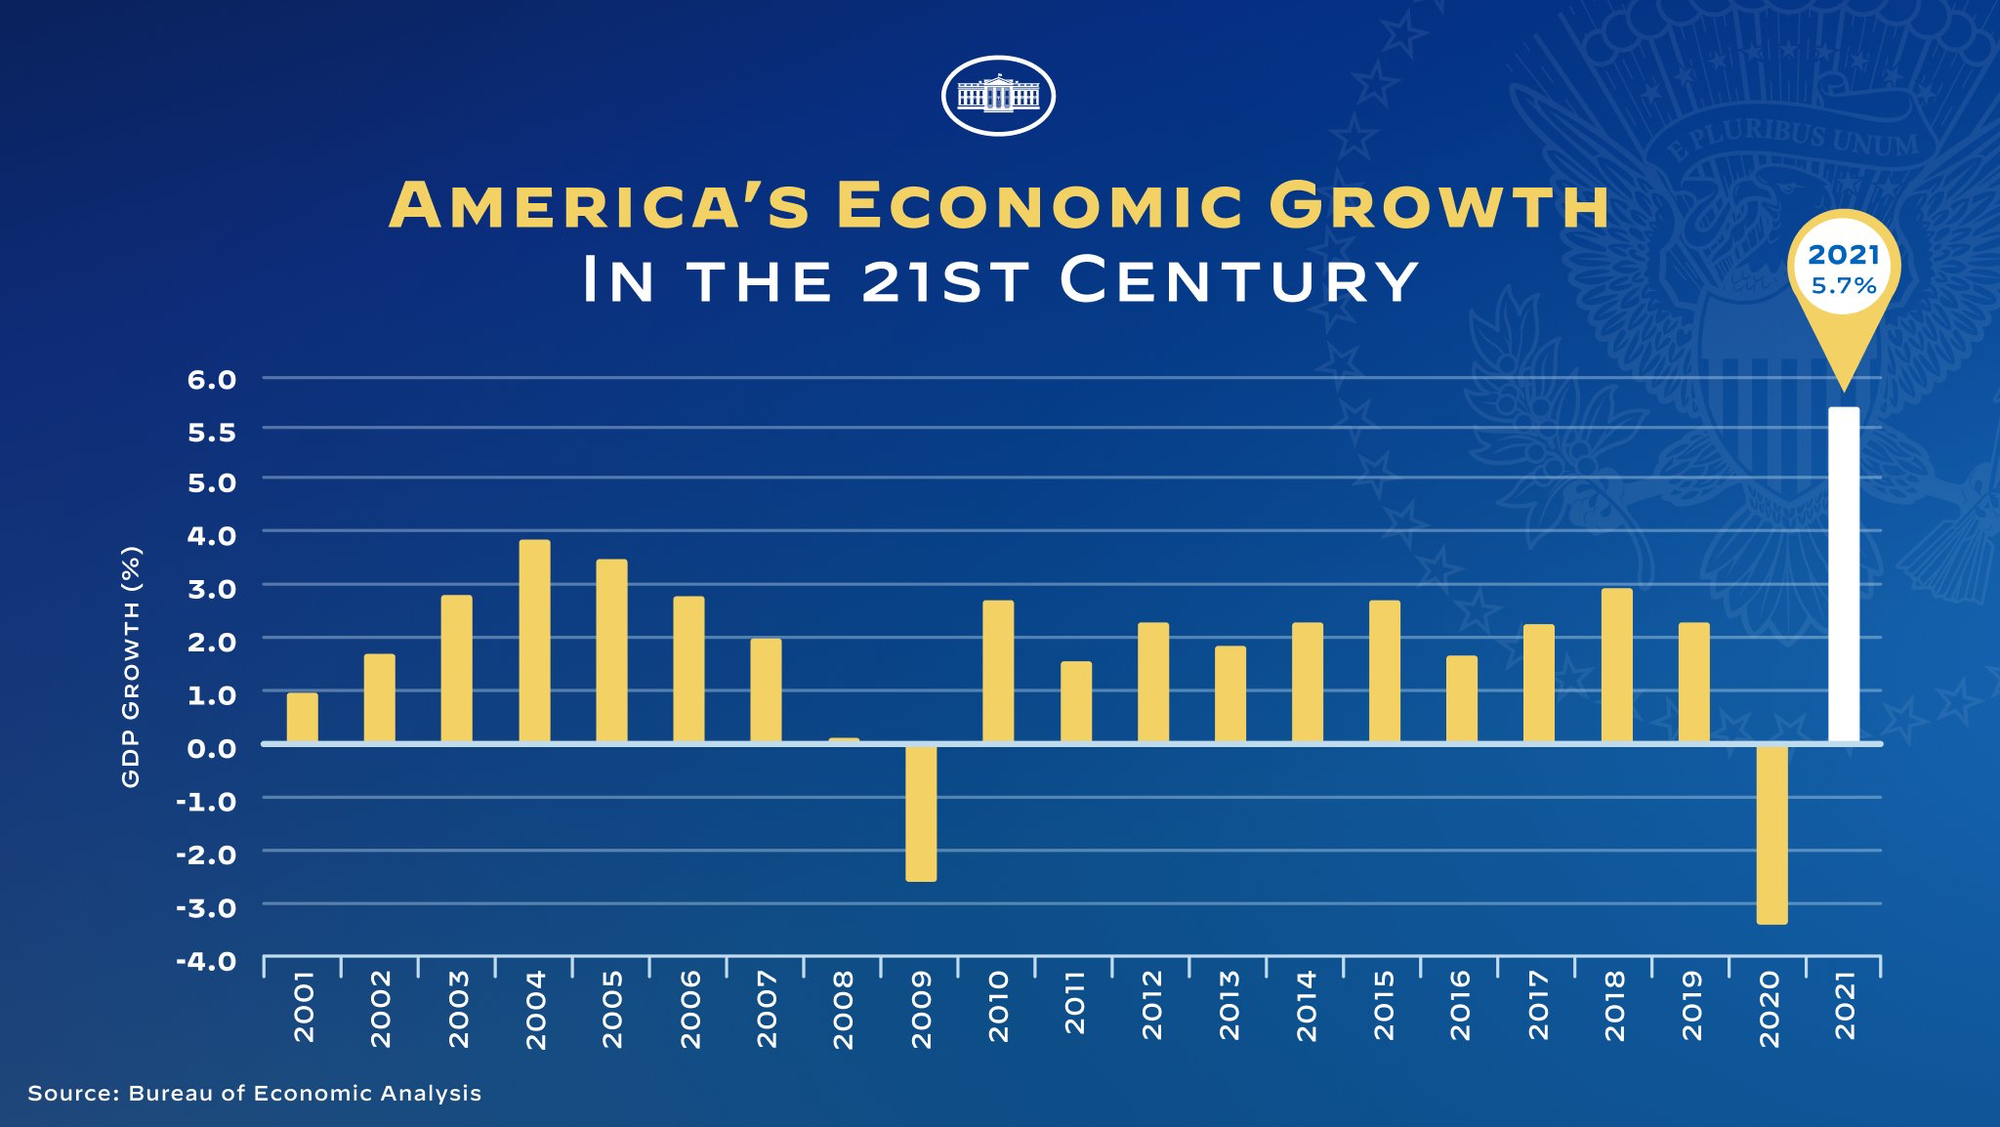
\includegraphics[width = 0.8\textwidth]{Lie-WhiteHouse.png} \\ }
  \only<2>{ 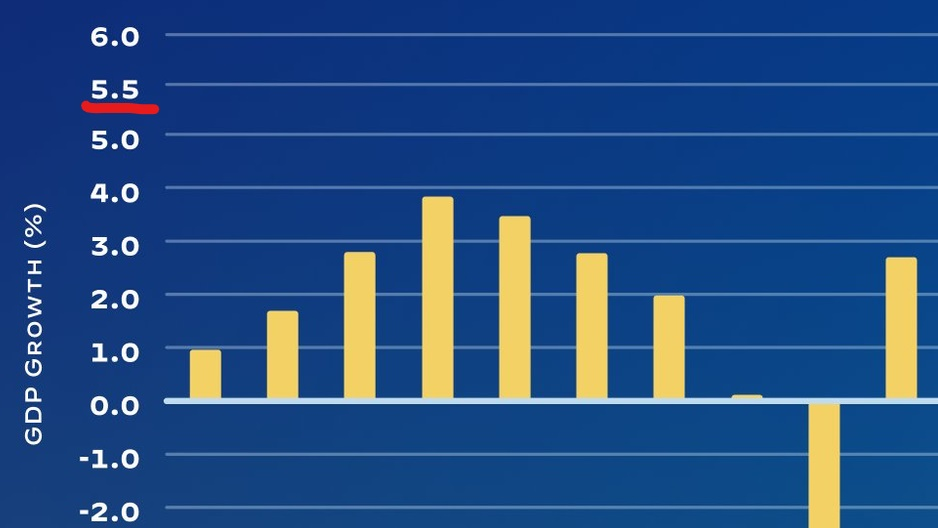
\includegraphics[width = 0.8\textwidth]{Lie-WhiteHouse-zoom.jpg} \\ }
  \only<3>{ \textbf{Initial} version \\ }
  \only<3>{ 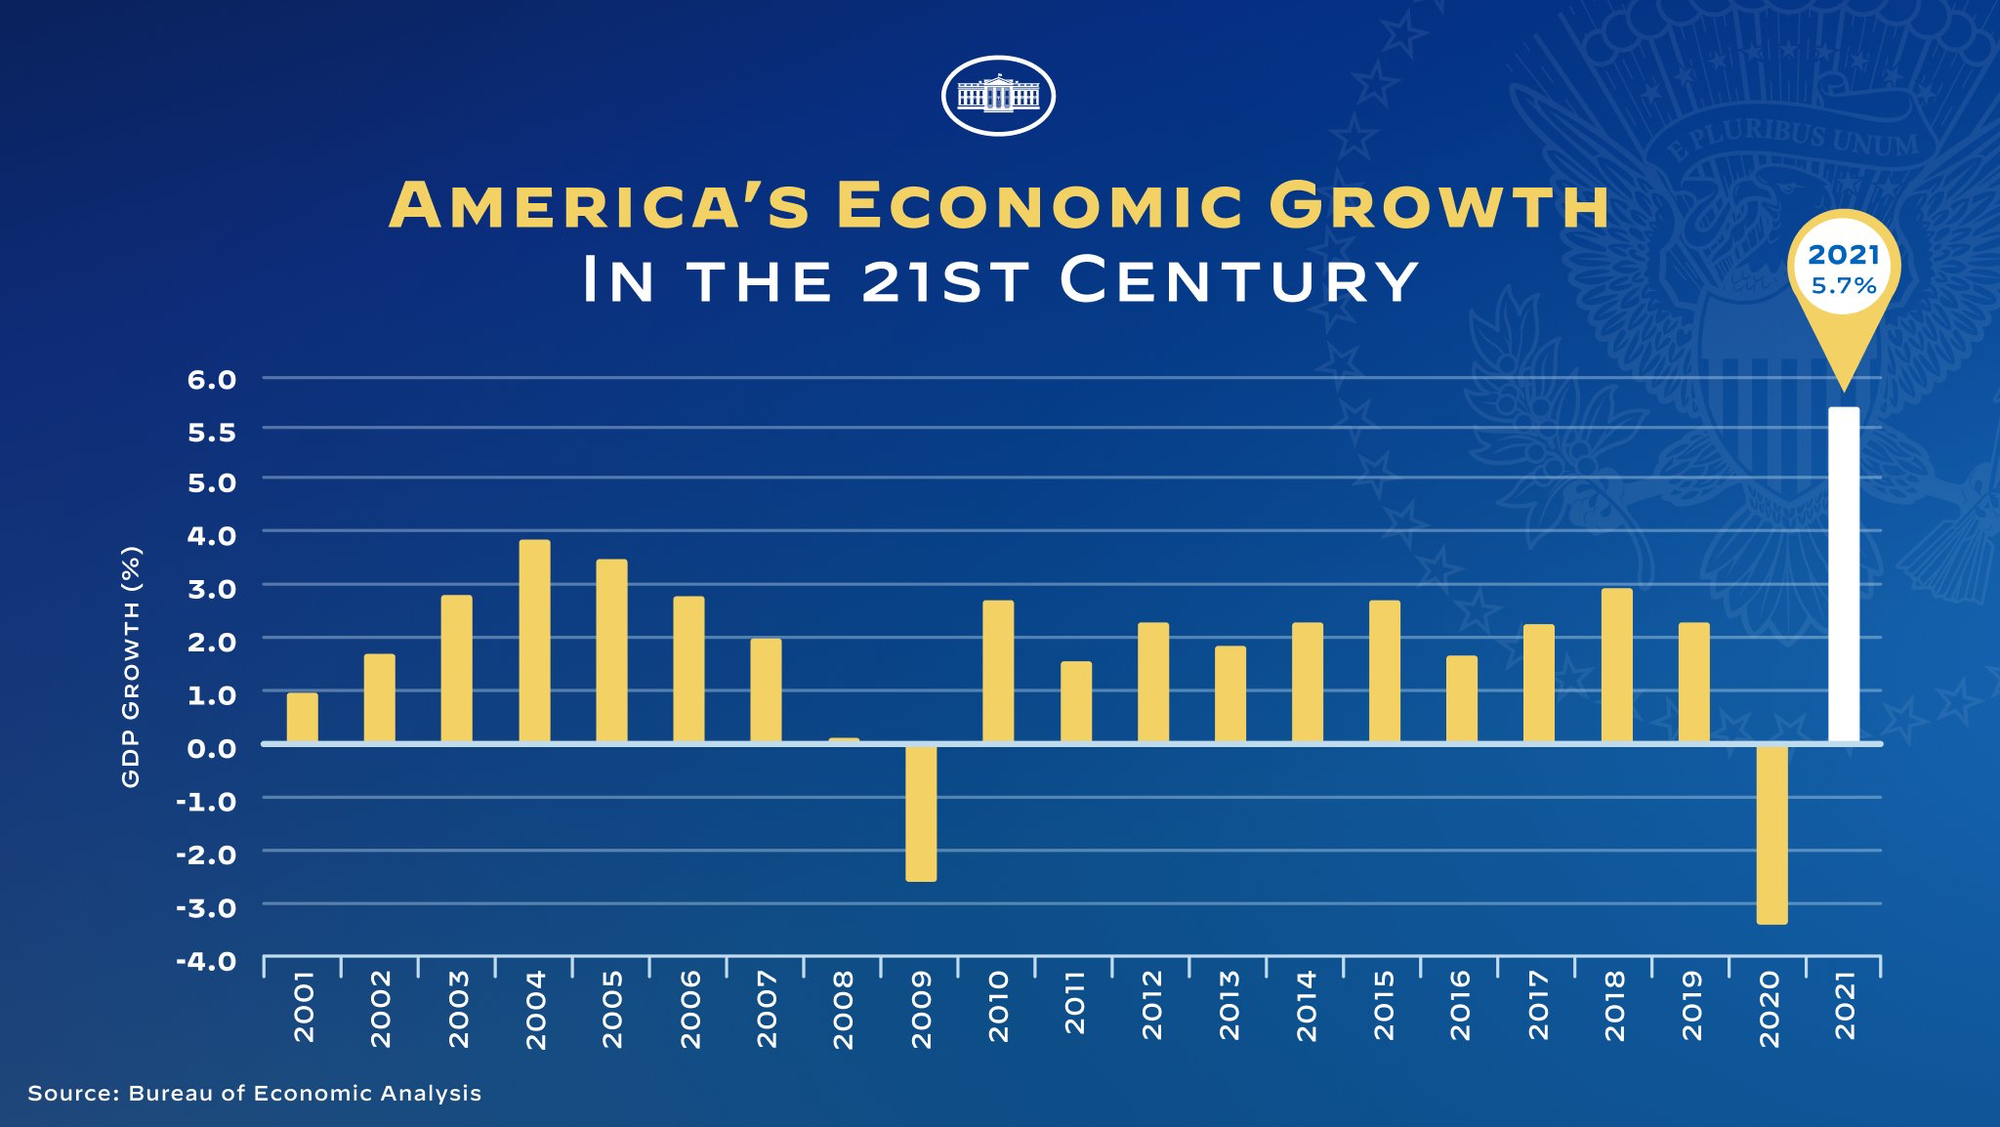
\includegraphics[width = 0.8\textwidth]{Lie-WhiteHouse.png} \\ }
  \only<4>{ \textbf{Correct} version \\ }
  \only<4>{ 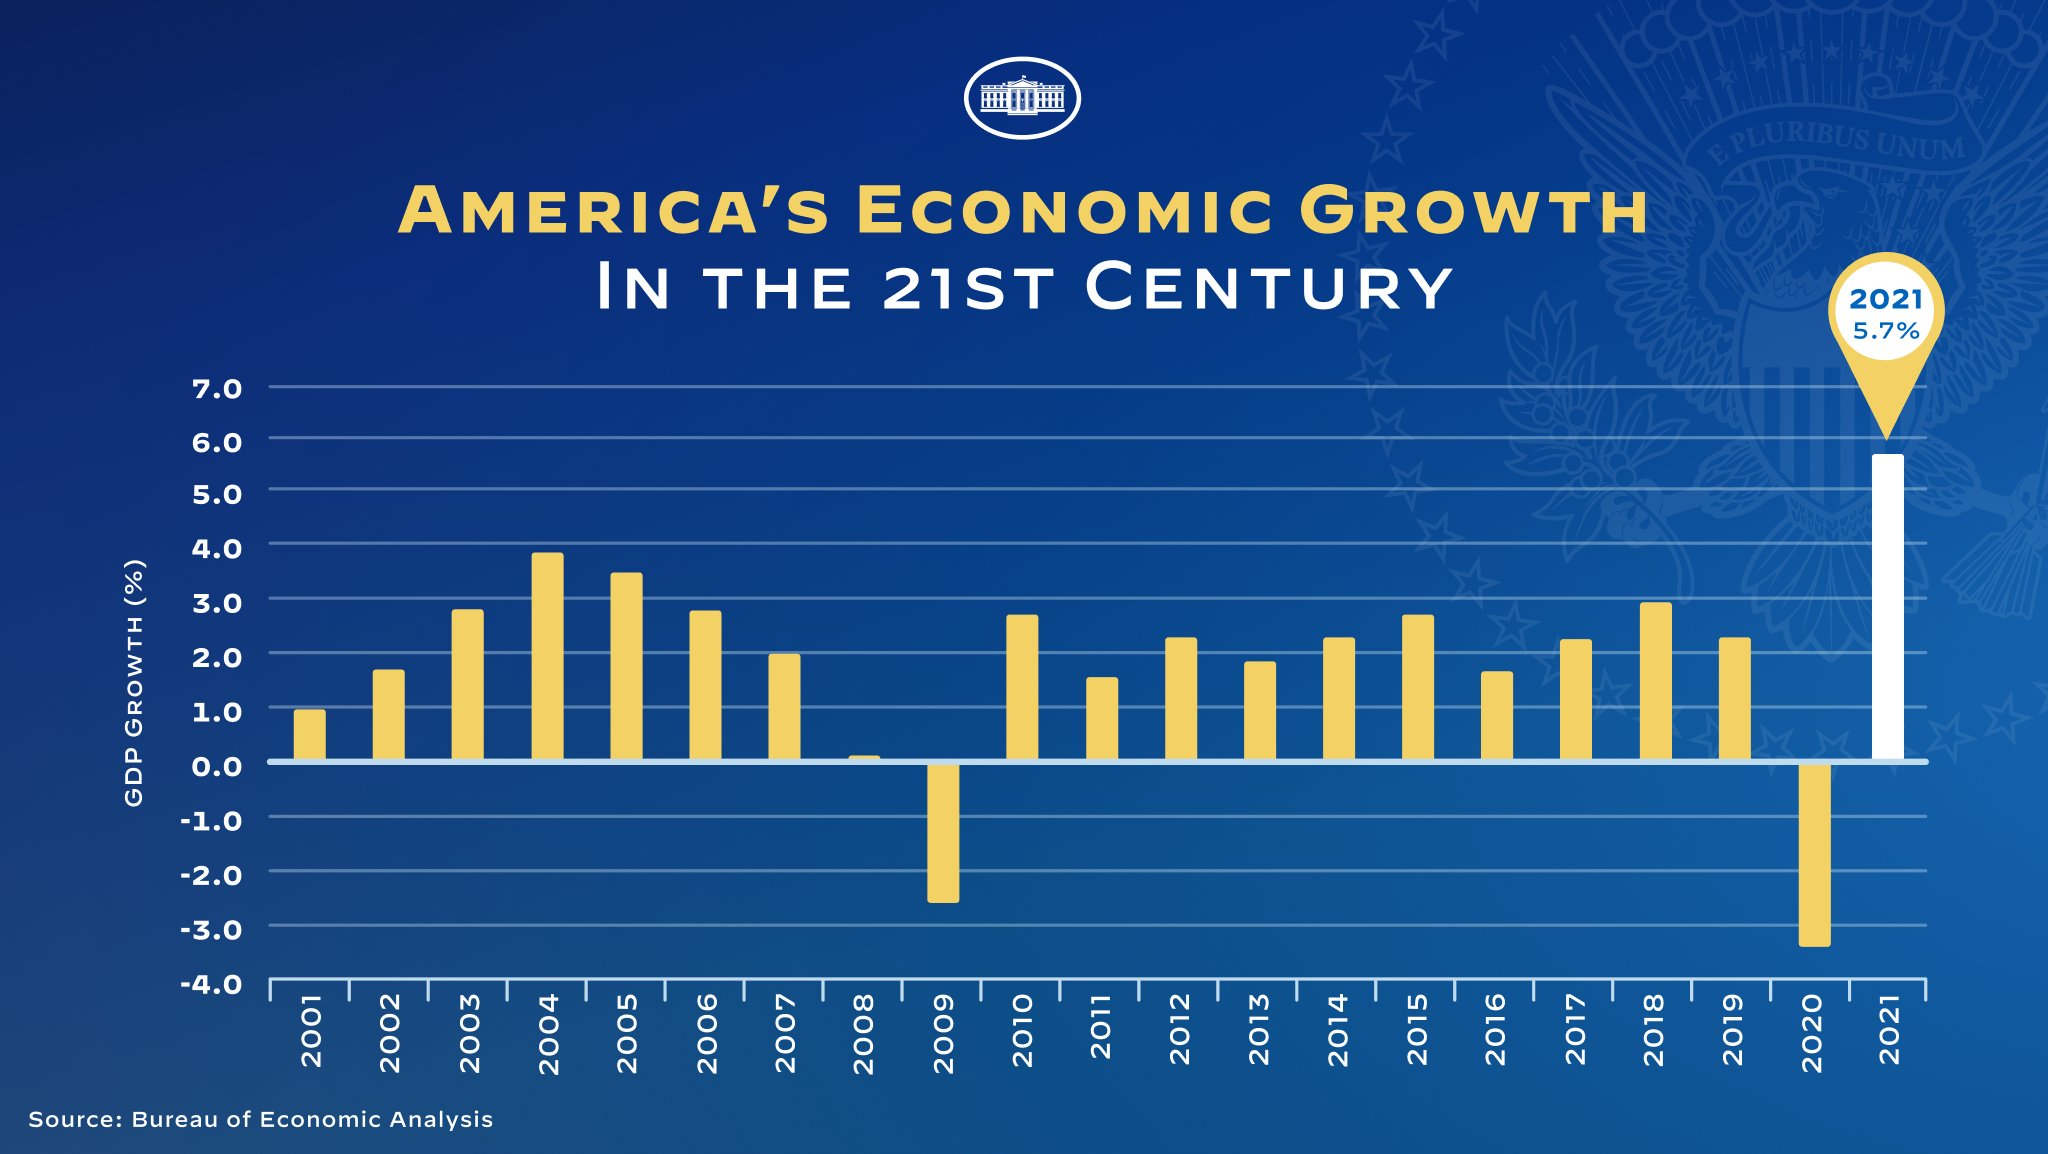
\includegraphics[width = 0.8\textwidth]{Lie-WhiteHouse-correct.jpg} \\ }
  \only<1-4>{\textcolor{gris}{\footnotesize{Source: \href{https://twitter.com/WhiteHouse/status/1486709480351952901/photo/1}{The White House (twitter)}}}}
\end{itemize}
\end{center}
\end{frame}
% See also https://www.marketwatch.com/story/white-house-cant-even-get-good-news-right-11643382733



\begin{frame}
\frametitle{\textcolor{brique}{[-\textbf{Rule \#2-bis: Play with shape!}-]}}
\begin{center}
\begin{itemize}
  \only<1>{First graphic again}
  \only<1>{ 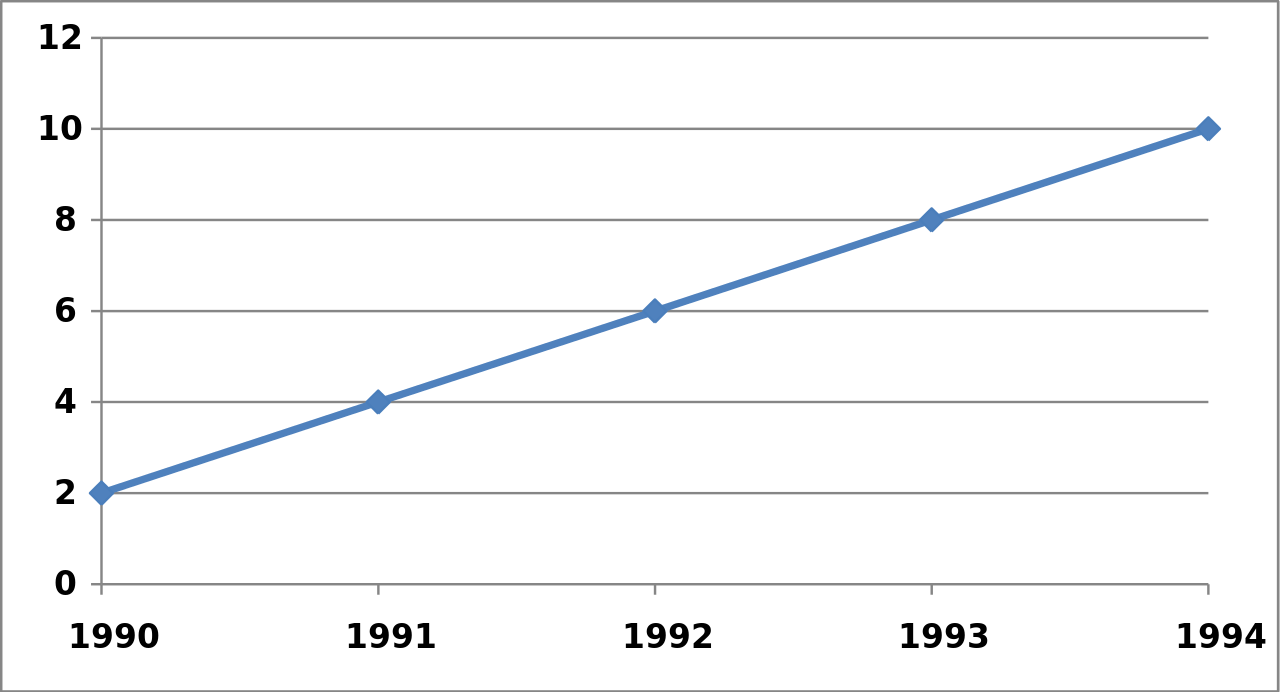
\includegraphics[width = 0.8\textwidth]{Line_graph1.png}}
  \only<2>{The same with a short \textbf{X}-axis}
  \only<2>{ 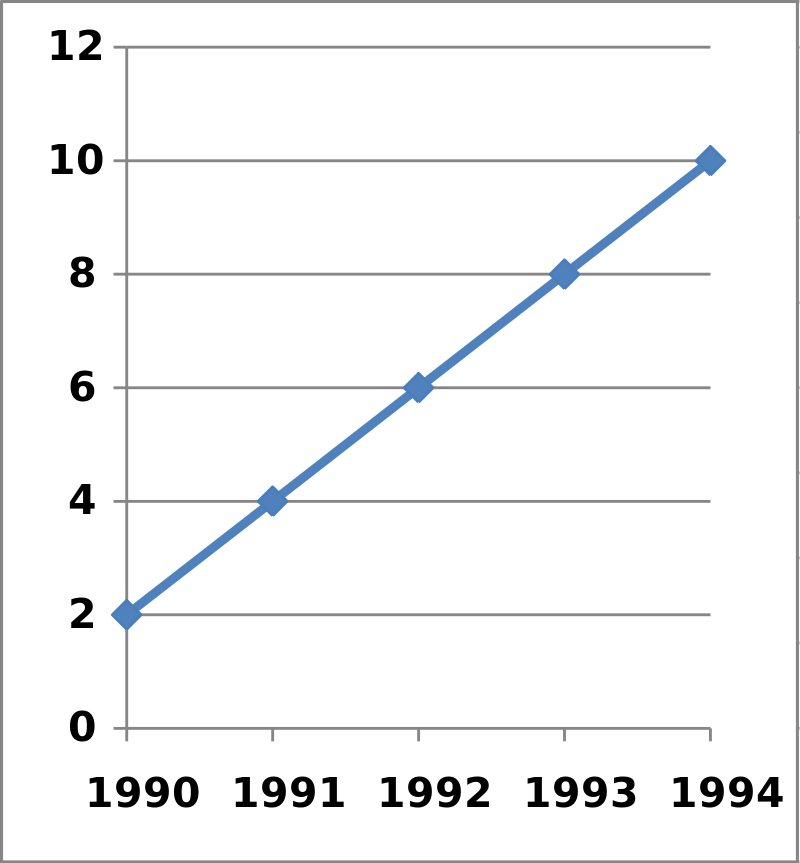
\includegraphics[width = 0.4\textwidth]{Line_graph1-3.png}}
  \only<3>{The same with a widespread \textbf{X}-axis and a short \textbf{Y}-axis }
  \only<3>{ 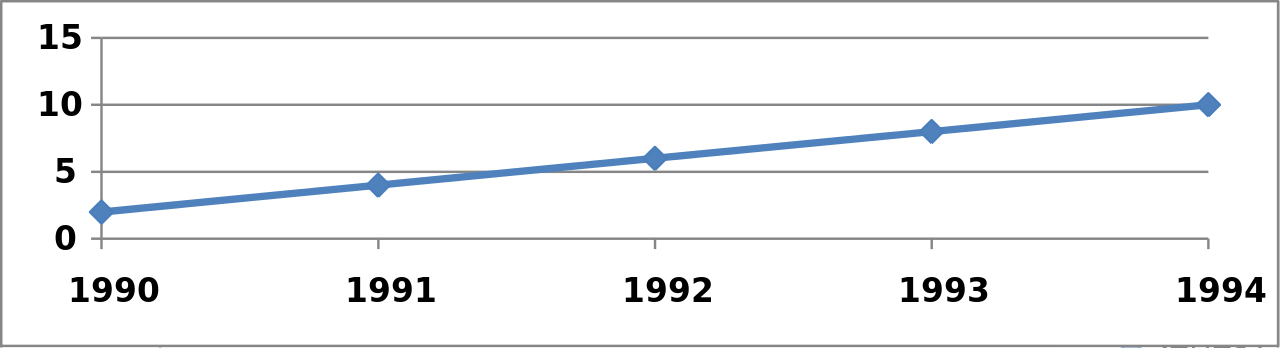
\includegraphics[width = 0.8\textwidth]{Line_graph1-4.png}}
\end{itemize}
\end{center}
\textcolor{gris}{\footnotesize{Source: \href{https://en.wikipedia.org/wiki/Misleading_graph}{Wikipedia: Misleading graph}}}
\end{frame}




%\begin{frame} % Cover slide
%\frametitle{\textcolor{brique}{[-\textbf{Rule \#2: Example}-]}}
%\begin{figure}[h]
%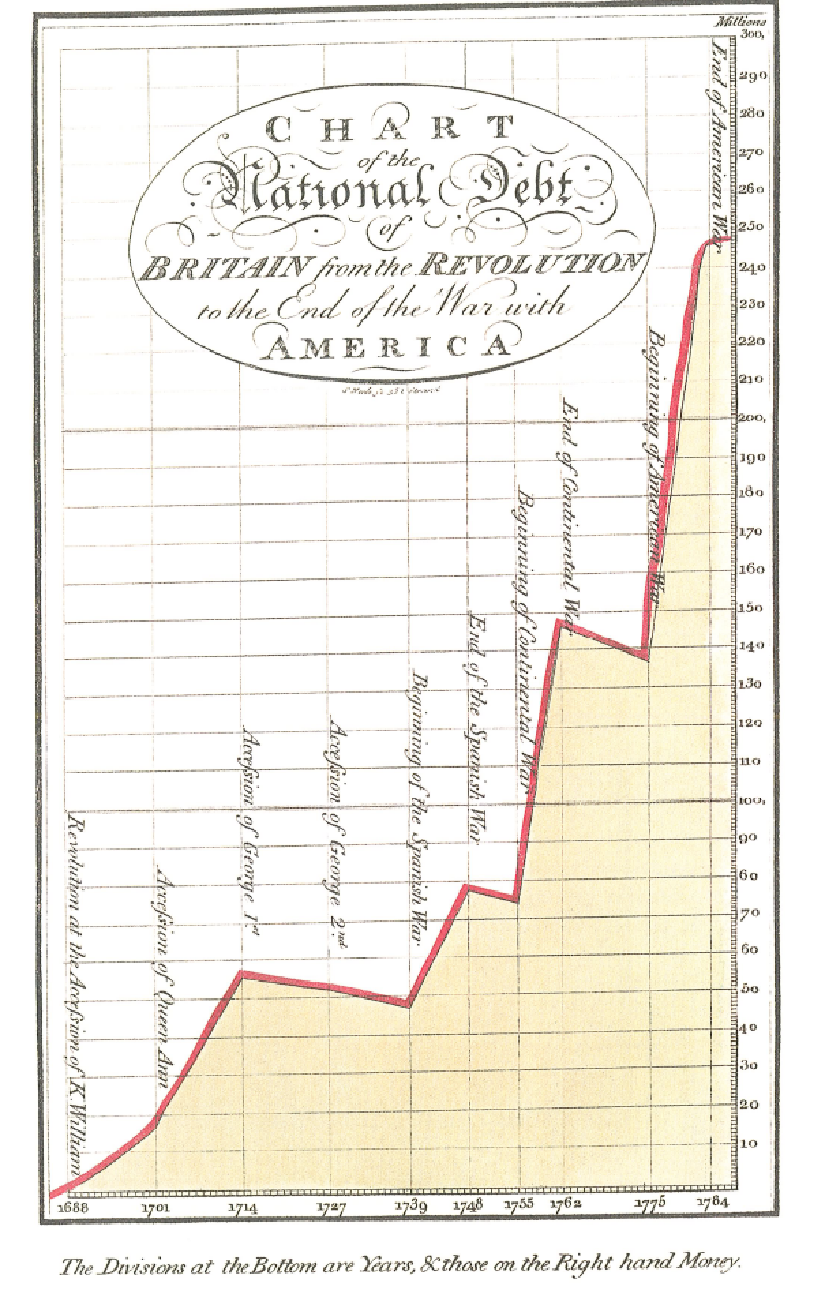
\includegraphics[width = 0.5\textheight, angle = -1]{GovernmentSpending1.pdf}
%\caption{Source : \cite{Tufte2001} from Playfair(1786).}
%\end{figure}
%\end{frame}
%
%\begin{frame} % Cover slide
%\frametitle{\textcolor{brique}{[-\textbf{Rule \#2-bis: Example}-]}}
%\begin{figure}[h]
%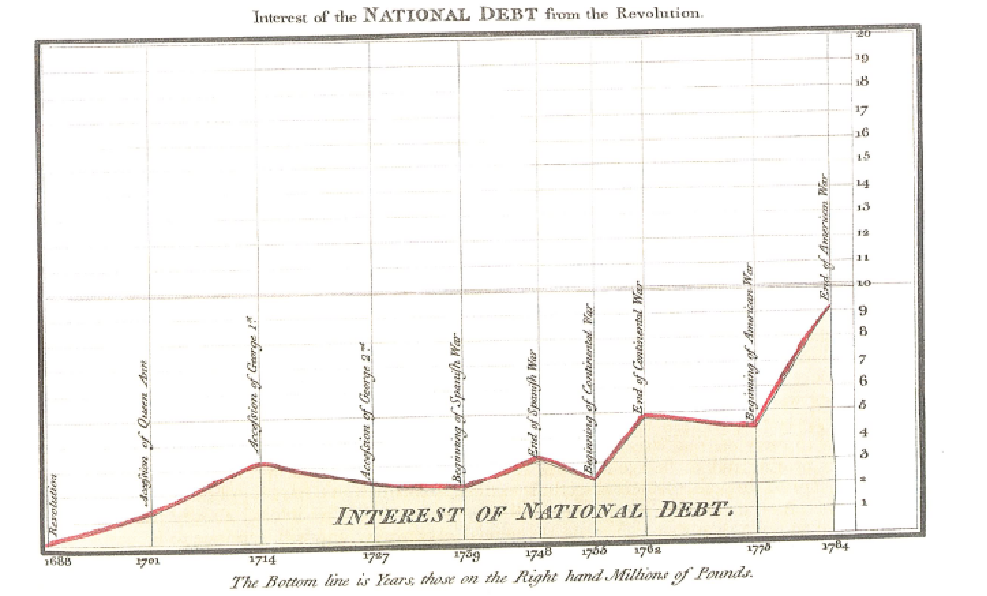
\includegraphics[width =0.8\textwidth, angle = -1]{GovernmentSpending2.pdf}
%\caption{Source : \cite{Tufte2001} from Playfair(1786).  }
%\end{figure}
%\end{frame}


\begin{frame} % Cover slide
\frametitle{\textcolor{brique}{[-\textbf{Applying Rule \#2-bis: Coronavirus example}-]}}
\begin{center}
\begin{itemize}
\item[]
  \only<1>{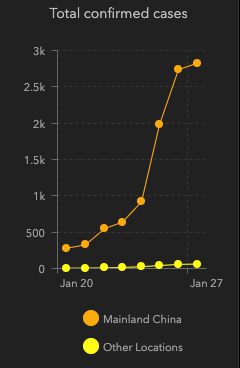
\includegraphics[width =0.3\textwidth]{john-hopkins-confirmed-cases-coronavirus.png} \\ }
  \only<1>{ Source: \href{https://www.sciencealert.com/this-online-dashboard-tracks-the-global-spread-of-the-wuhan-coronavirus-in-real-time}{Science Alert (2020)}}
  \only<2>{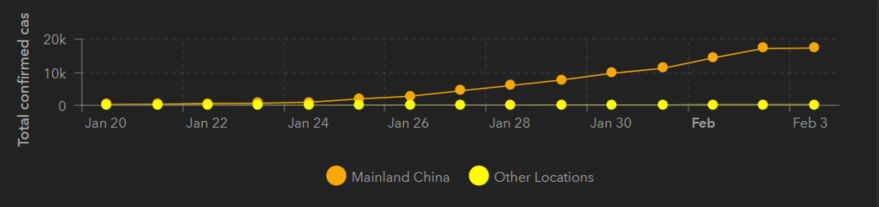
\includegraphics[width =0.9\textwidth]{john-hopkins-confirmed-cases-coronavirus2.png} \\ }
  \only<2>{Source: \href{https://gisanddata.maps.arcgis.com/apps/opsdashboard/index.html/bda7594740fd40299423467b48e9ecf6}{John Hopkins CSSE (2020)}}
\end{itemize}
\end{center}
\end{frame}


%
%\begin{frame} % Cover slide
%\frametitle{\textcolor{brique}{[-\textbf{Rule \#2-bis: Subtle things...}-]}}
%Which sample has the highest correlation?
%\begin{center}
%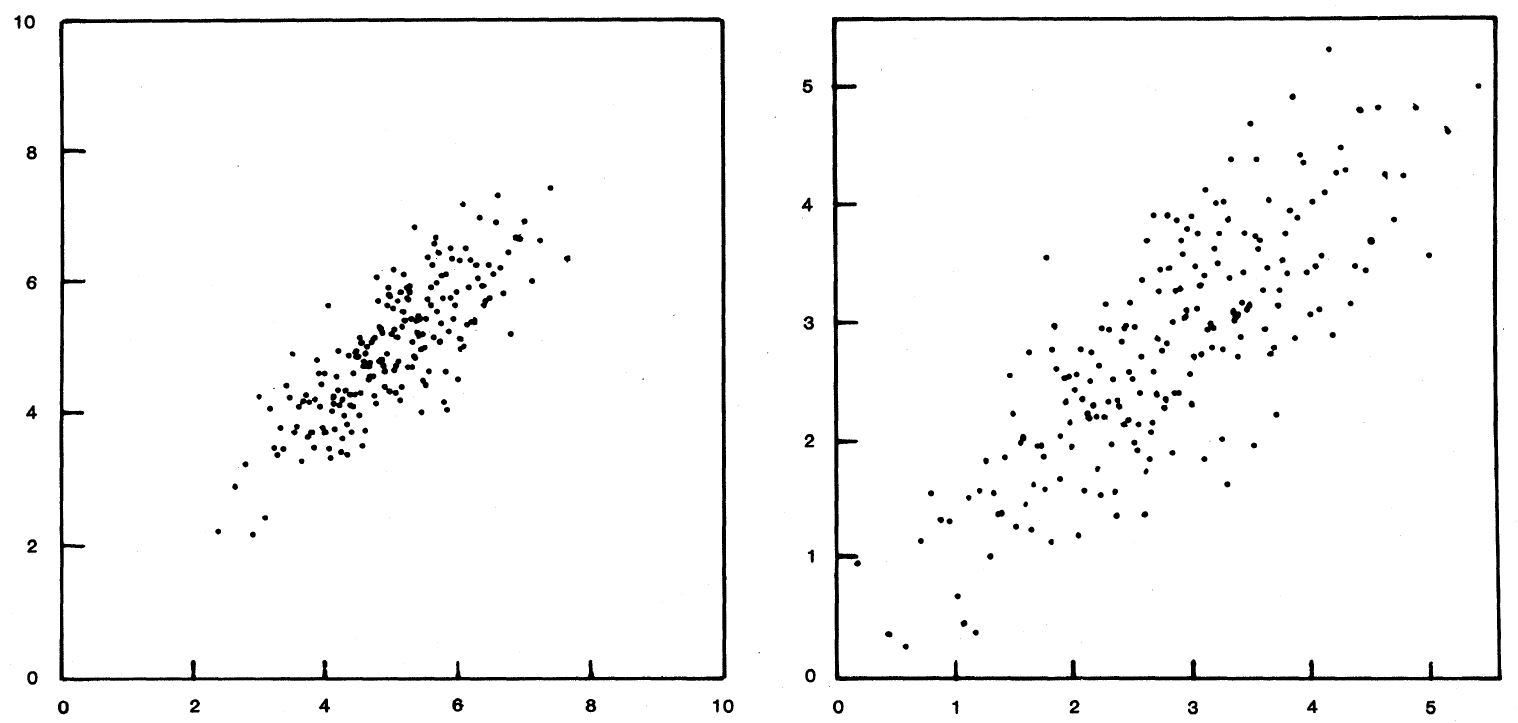
\includegraphics[width = 1.0\textwidth]{ScalesScatterplotConcentrationCleveland.JPG}
%\end{center}
%From \cite{Cleveland1982}
%% R^2 = 0.8 in each cell...
%\end{frame}
%
%



%\begin{frame} % Cover slide
%\frametitle{\textcolor{brique}{[- \textbf{Rule \#2 bis: Reverse the scale/units} -]}}
%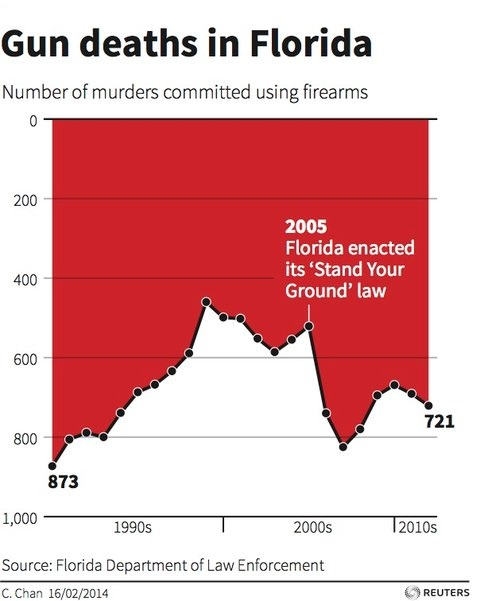
\includegraphics[width = 0.55\textwidth]{GunsDeathReversed.jpg}
%\textcolor{gris}{\footnotesize{\href{https://www.livescience.com/45083-misleading-gun-death-chart.html}{LiveScience.com}}}
%\end{frame}
%
%
%\begin{frame} % Cover slide
%\frametitle{\textcolor{brique}{[- \textbf{Rule \#2 bis: Reverse the scale/units} -]}}
%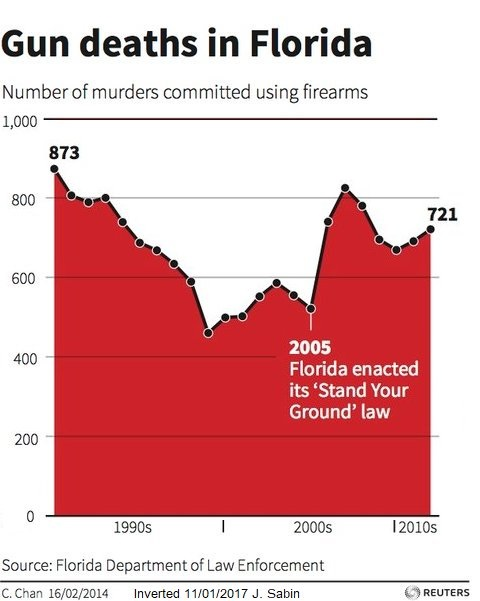
\includegraphics[width = 0.55\textwidth]{GunsDeathRight.jpg}
%\textcolor{gris}{\footnotesize{\href{https://www.livescience.com/45083-misleading-gun-death-chart.html}{LiveScience.com}}}
%\end{frame}
%

\section{Rule 3}

\begin{frame} % Cover slide
\frametitle{\textcolor{brique}{[- \textbf{Rule \#3: Use double axes! } -]}}
An apparently harmless example:

\begin{center}
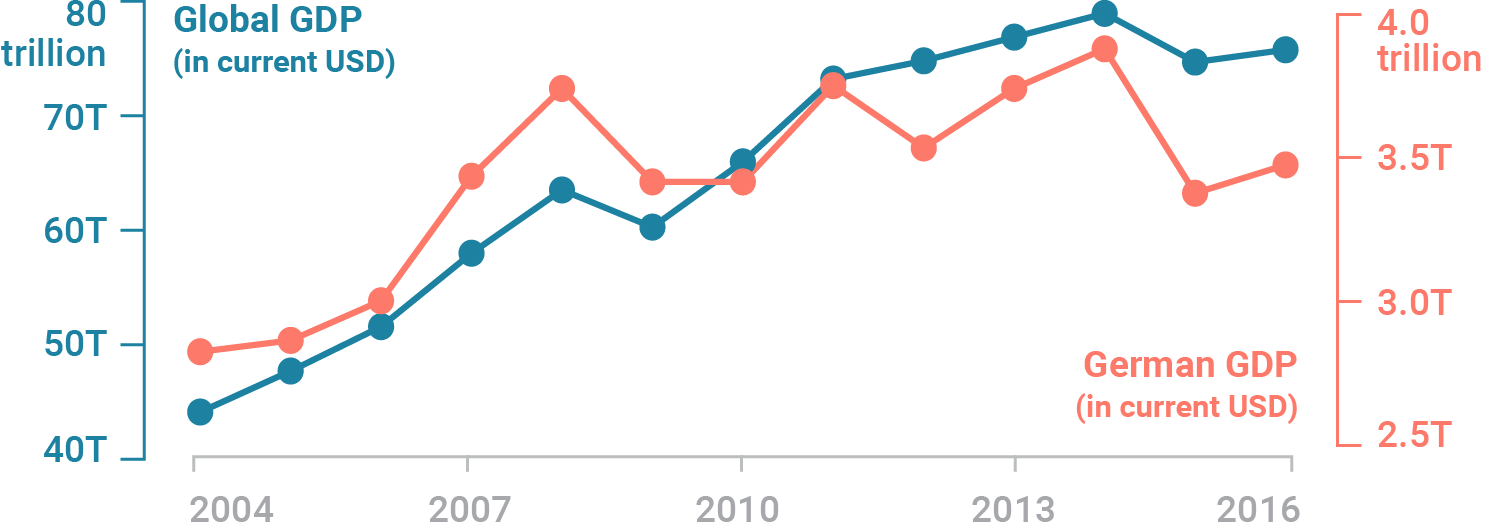
\includegraphics[width = 1.0\textwidth]{LCRost-dualaxis1.png}
\end{center}
\textcolor{gris}{\footnotesize{Source: \href{https://blog.datawrapper.de/dualaxis/index.html}{Lisa Charlotte Rost}, data from World bank}}
\end{frame}

\begin{frame} % Cover slide
\frametitle{\textcolor{brique}{[- \textbf{Rule \#3: Use double axes! } -]}}
Zero baseline are not aligned!

\begin{center}
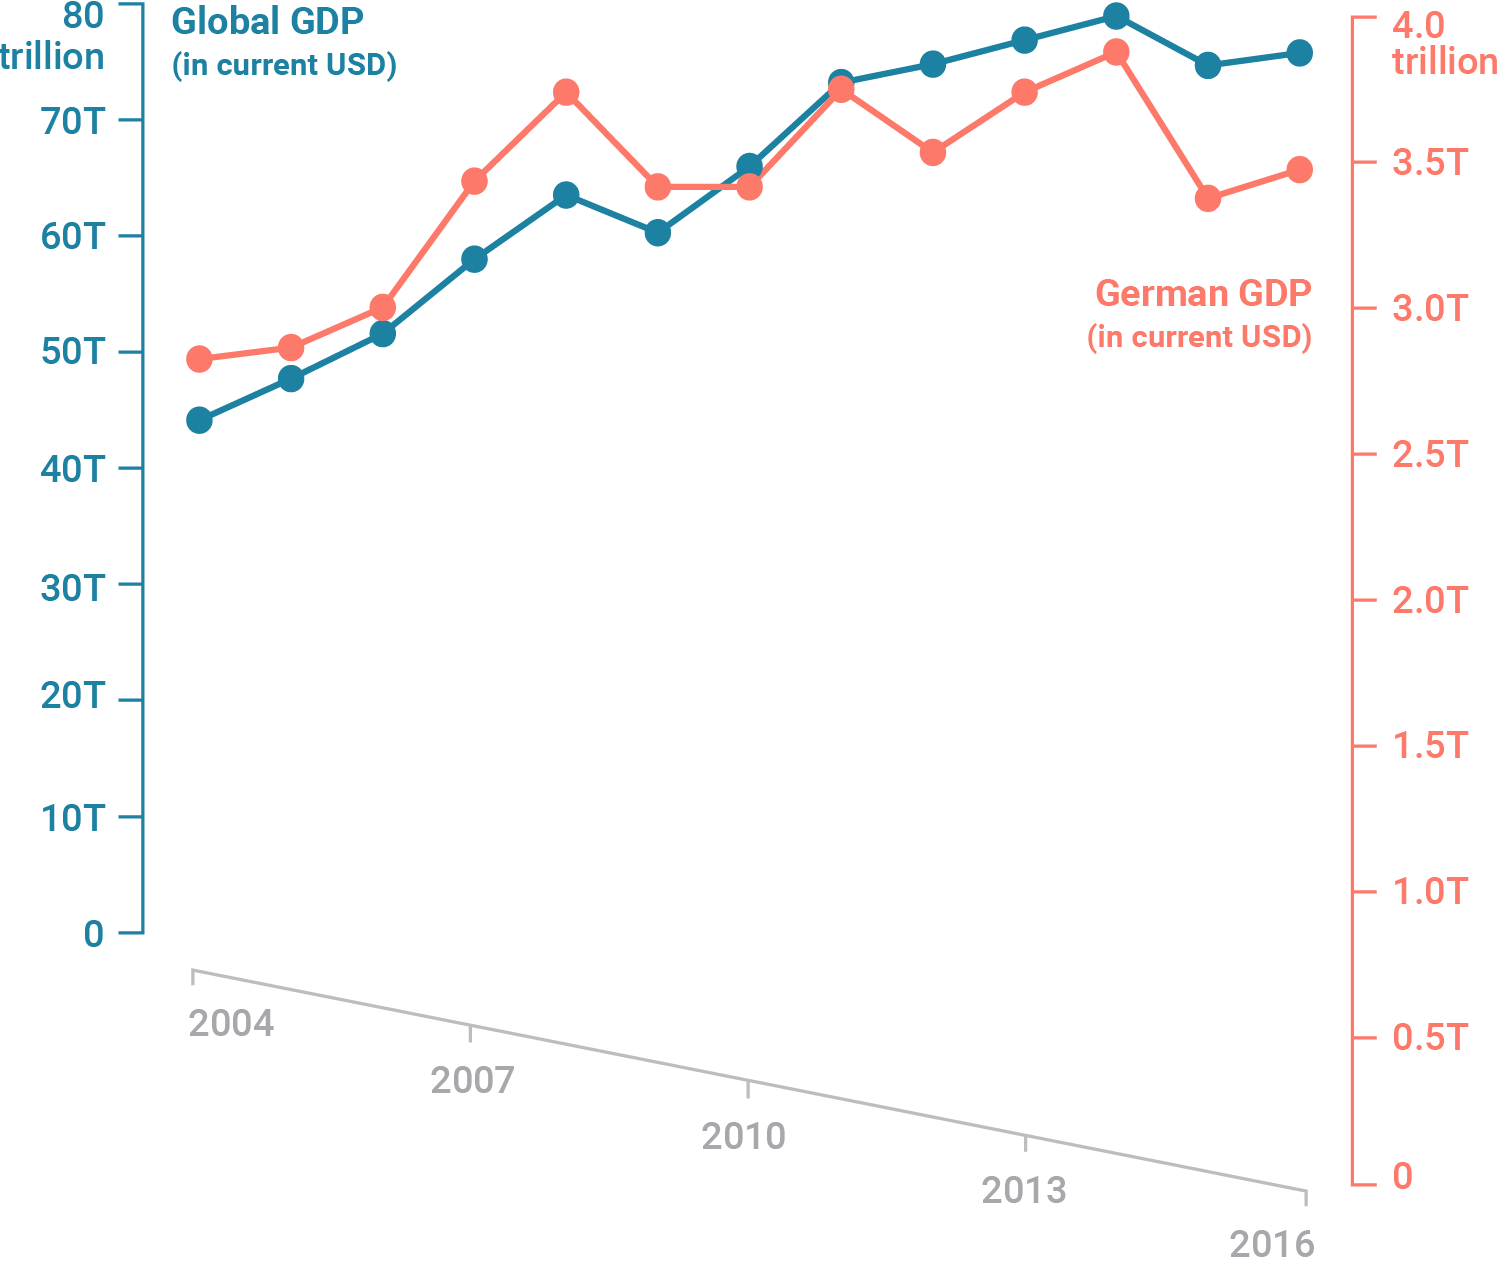
\includegraphics[width = 0.5\textwidth]{LCRost-dualaxis2.png}
\end{center}
\textcolor{gris}{\footnotesize{Source: \href{https://blog.datawrapper.de/dualaxis/index.html}{Lisa Charlotte Rost}, data from World bank}}
\end{frame}

\begin{frame} % Cover slide
\frametitle{\textcolor{brique}{[- \textbf{Rule \#3: Use double axes! } -]}}
Does aligned zero baselines solve the problem?
\begin{center}
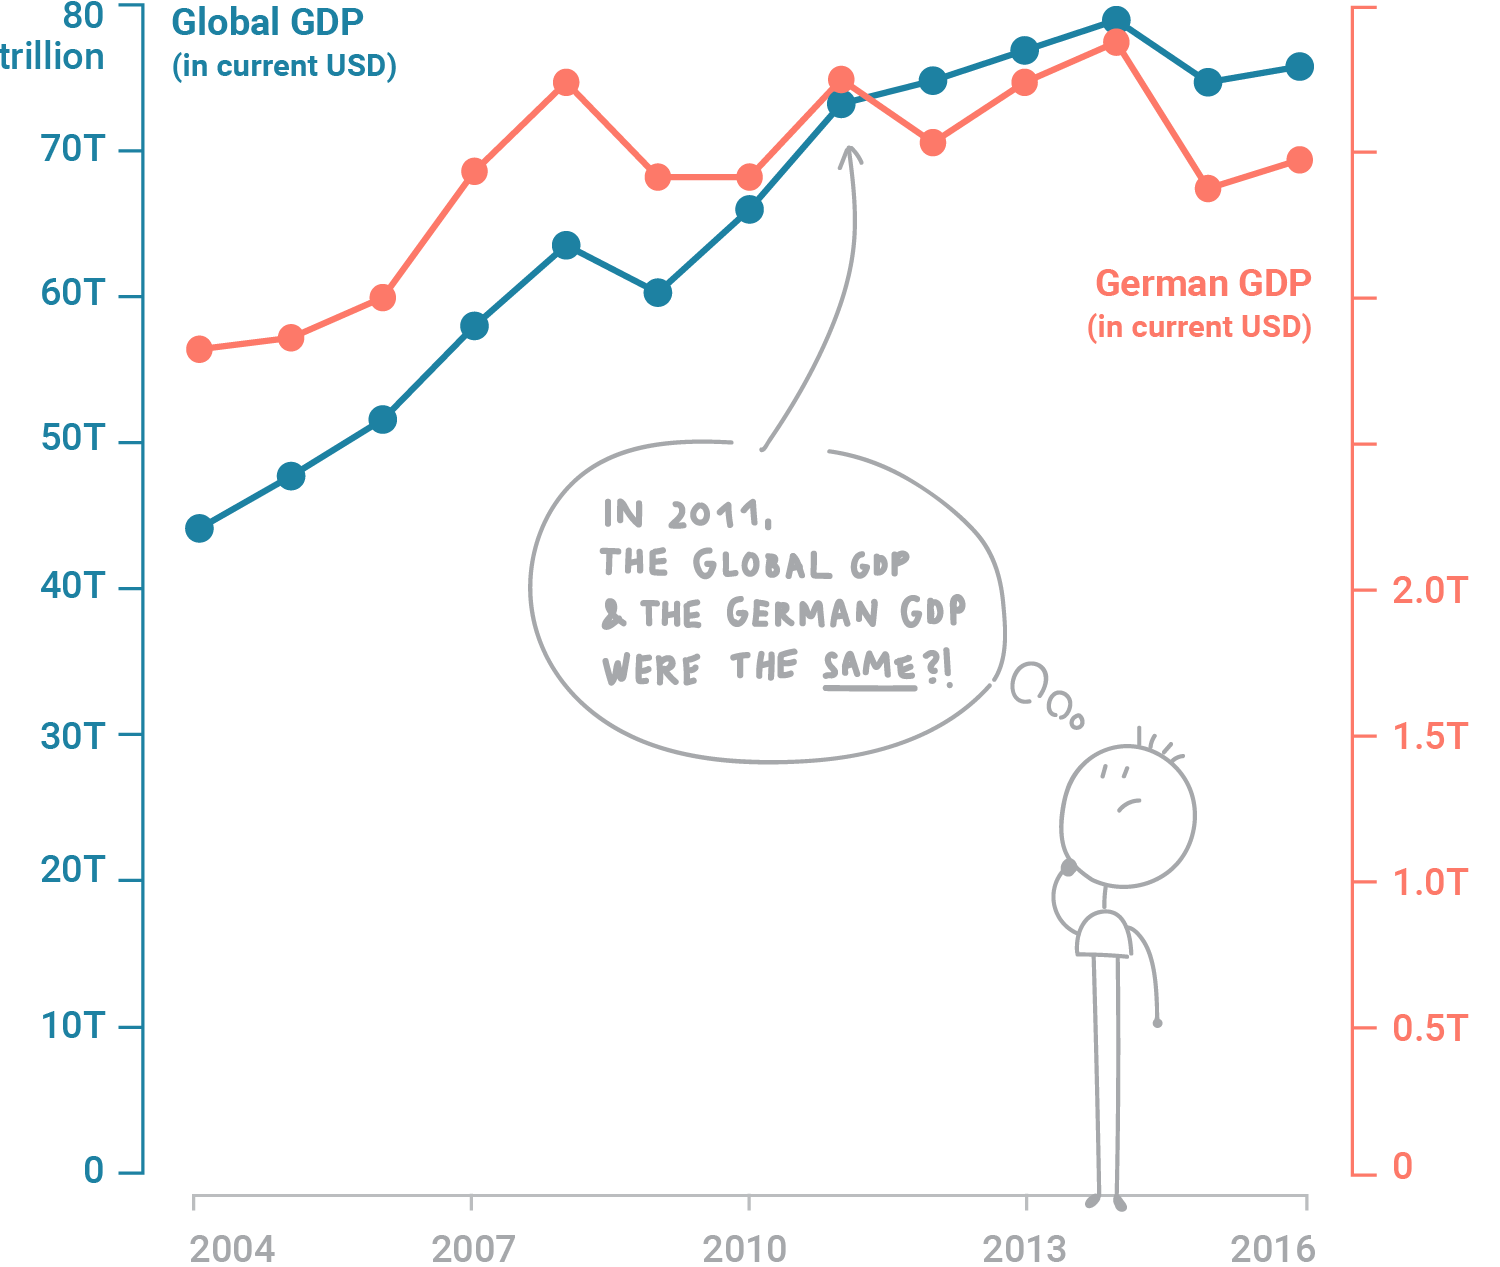
\includegraphics[width = 0.6\textwidth]{LCRost-dualaxis3.png}
\end{center}
\textcolor{gris}{\footnotesize{Source: \href{https://blog.datawrapper.de/dualaxis/index.html}{Lisa Charlotte Rost}, data from World bank}}
\end{frame}


\begin{frame} % Cover slide
\frametitle{\textcolor{brique}{[- \textbf{Rule \#3: Use double axes! } -]}}
When playing with scales, anything may happen...

\begin{center}
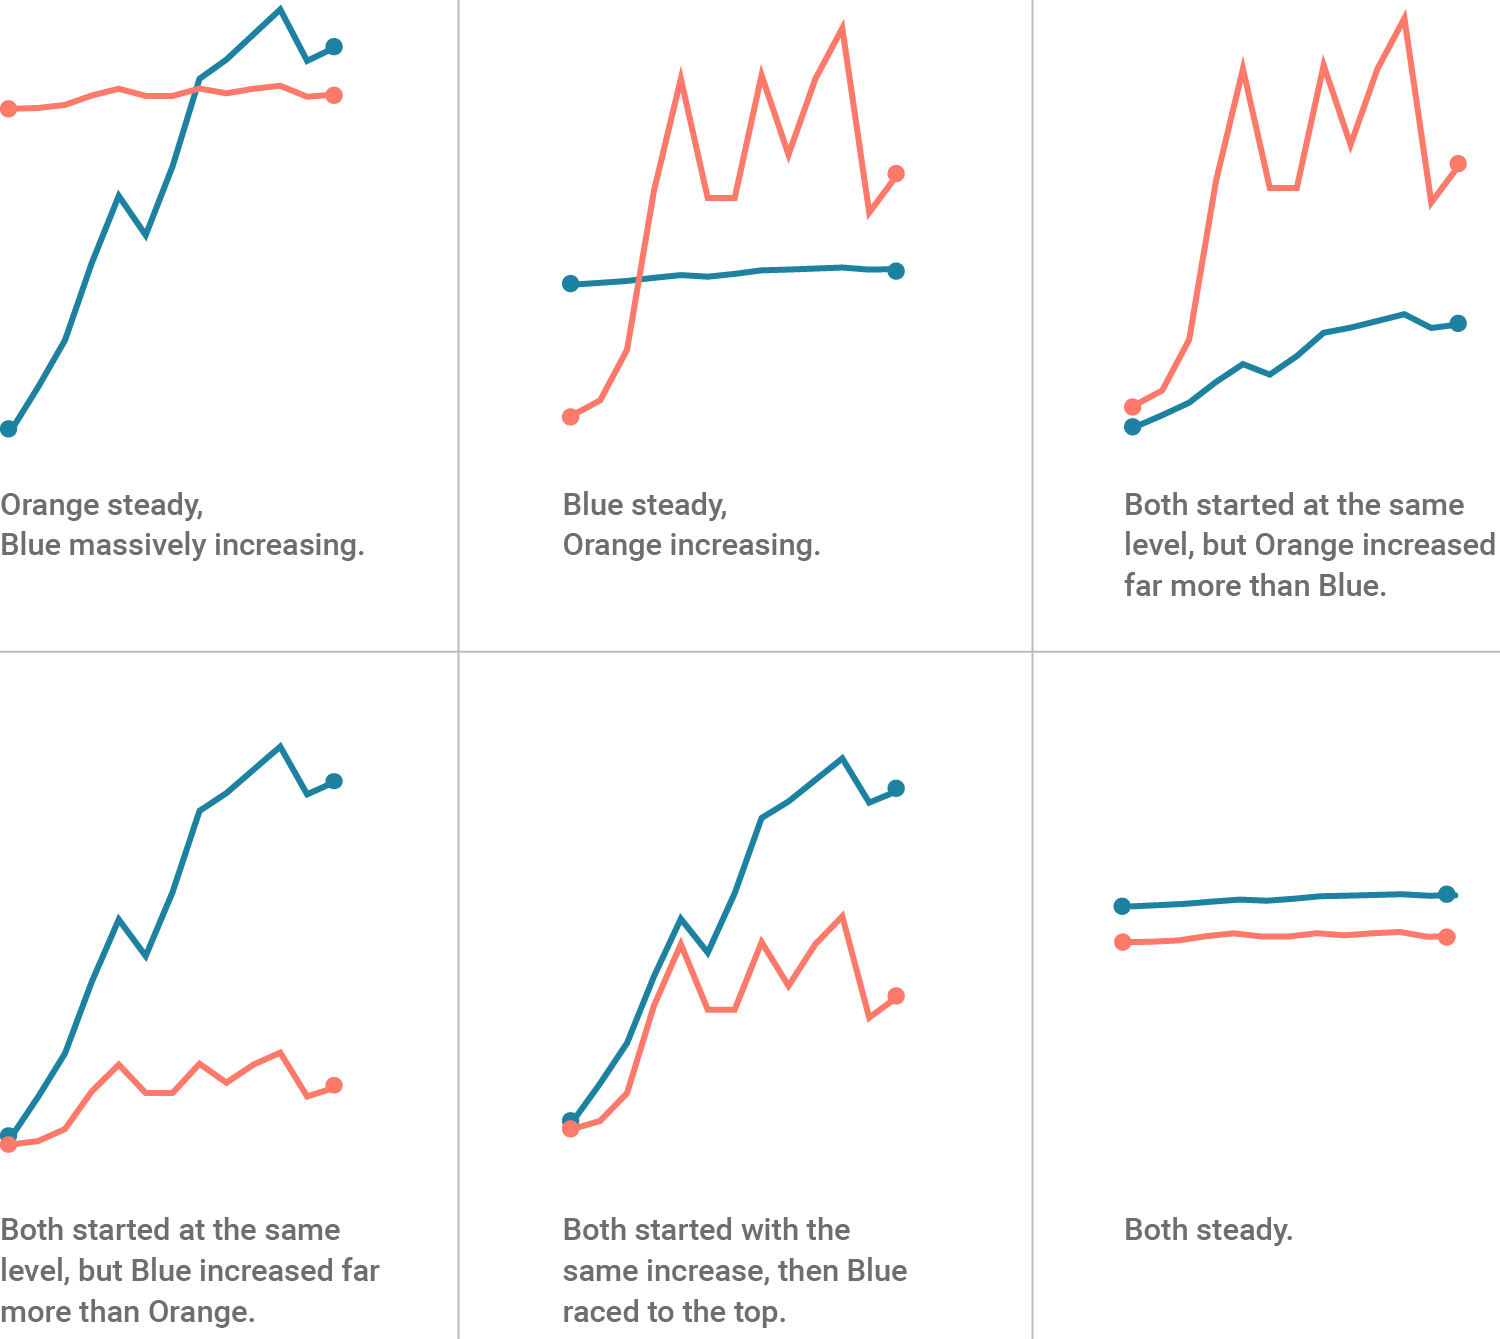
\includegraphics[width = 0.55\textwidth]{LCRost-dualaxisCrazy.png}
\end{center}
\textcolor{gris}{\footnotesize{Source: \href{https://blog.datawrapper.de/dualaxis/index.html}{Lisa Charlotte Rost}, data from World bank}}
\end{frame}


\begin{frame} % Cover slide
\frametitle{\textcolor{brique}{[- \textbf{Rule \#3: Use double axes! } -]}}
Solution 1: Two graphs
\begin{center}
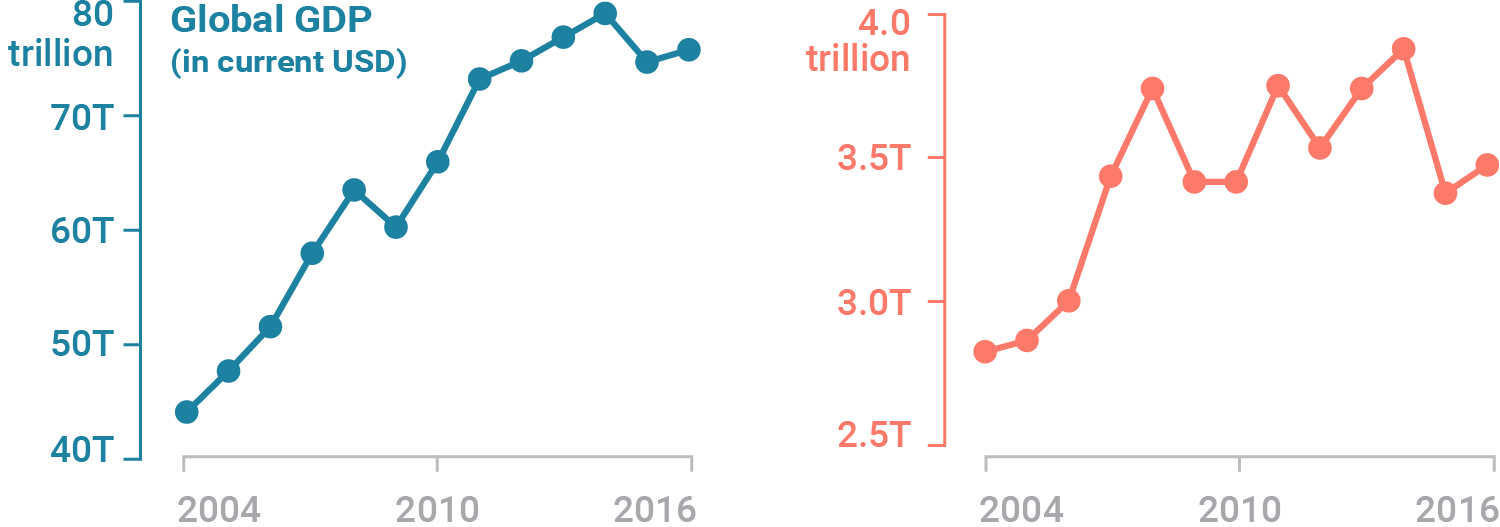
\includegraphics[width = 0.6\textwidth]{LCRost-dualaxisSolution1.png}
\end{center}
\textcolor{gris}{\footnotesize{Source: \href{https://blog.datawrapper.de/dualaxis/index.html}{Lisa Charlotte Rost}, data from World bank}}
\end{frame}

\begin{frame} % Cover slide
\frametitle{\textcolor{brique}{[- \textbf{Rule \#3: Use double axes! } -]}}
Solution: Indexes
\begin{center}
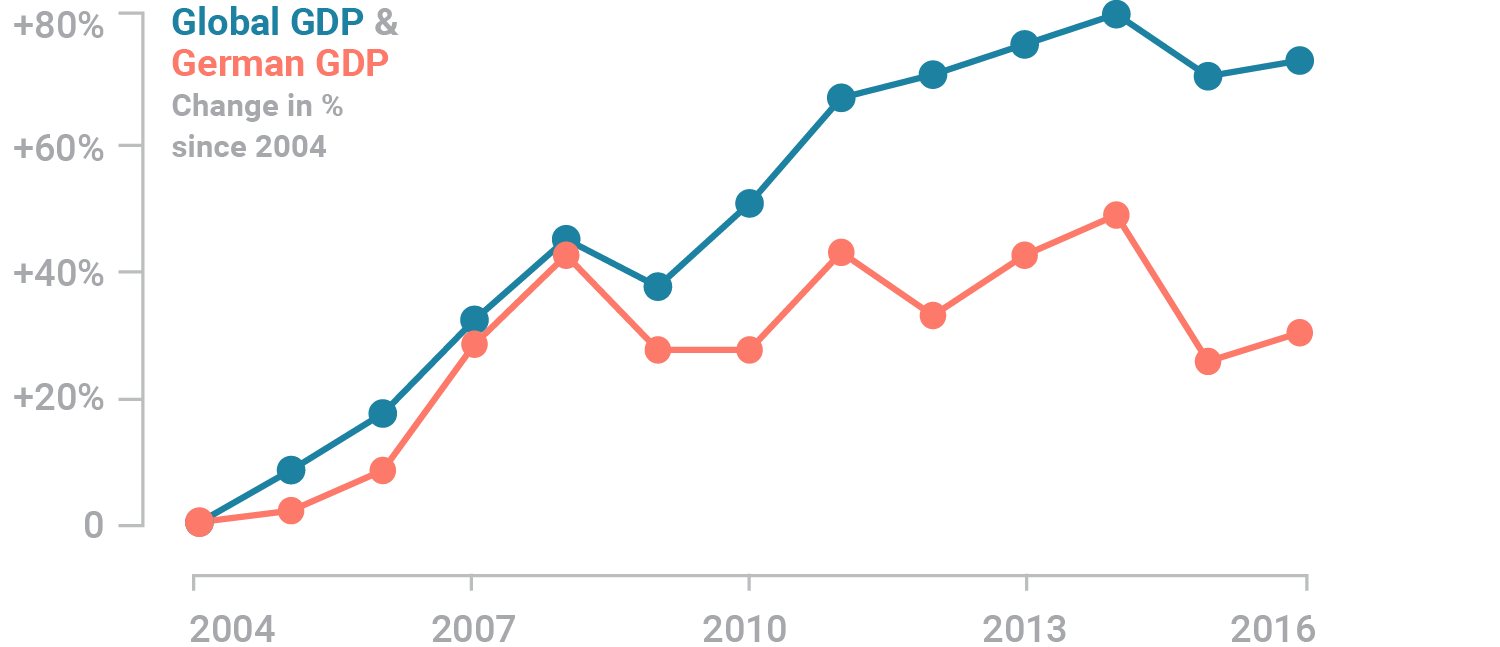
\includegraphics[width = 0.75\textwidth]{LCRost-dualaxisSolution2.png}
\end{center}
The German GDP and the global GDP \textbf{are not} growing at the same rate since 2008! \\
\textcolor{gris}{\footnotesize{Source: \href{https://blog.datawrapper.de/dualaxis/index.html}{Lisa Charlotte Rost}, data from World bank}}
\end{frame}




\begin{frame}
\frametitle{\textcolor{brique}{[- \textbf{Rule \#3: Funny Examples} -]}}
\begin{center}
\begin{itemize}
  \only<1>{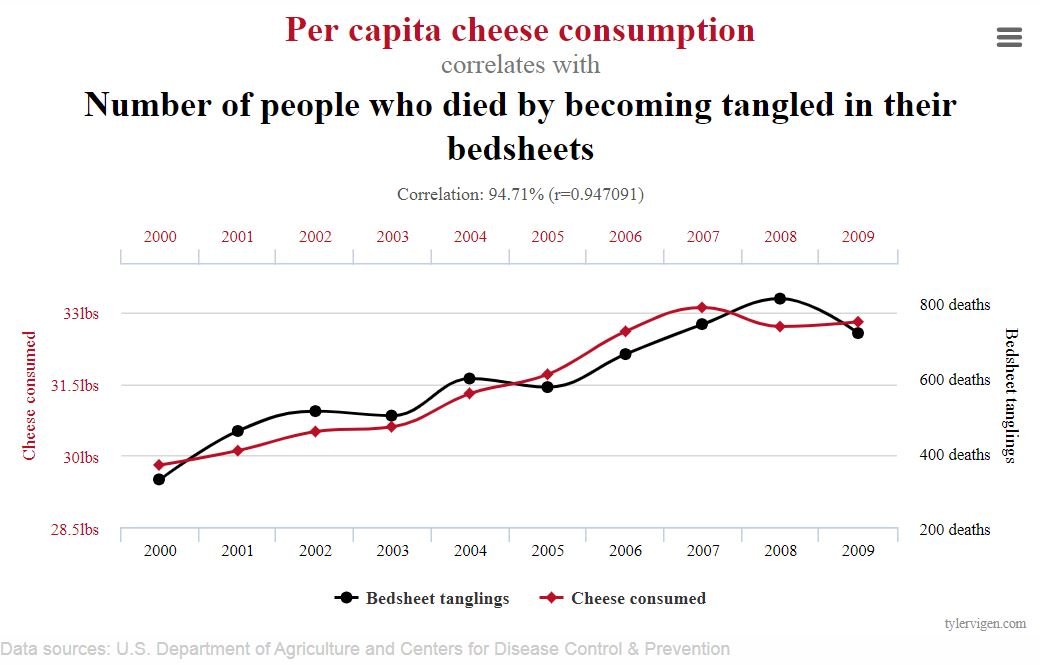
\includegraphics[width = 0.75\textwidth]{SpuriousCorrelations.JPG} \\ }
  \only<1>{\textcolor{gris}{\footnotesize{Source: \href{https://www.tylervigen.com/spurious-correlations}{ \textbf{Spurious Correlations}}}}}
\end{itemize}
\end{center}
\end{frame}

%\begin{frame}
%\frametitle{\textcolor{brique}{[- \textbf{Rule \#3: Examples } -]}}
%%%% SEARCH SNETENCE ON JSTOR :  graphic economic  site:https://www.jstor.org/
%\begin{center}
%\begin{itemize}
%  \only<1>{Glyphosate \textit{vs} Senile dementia\\ }
%  \only<1>{ 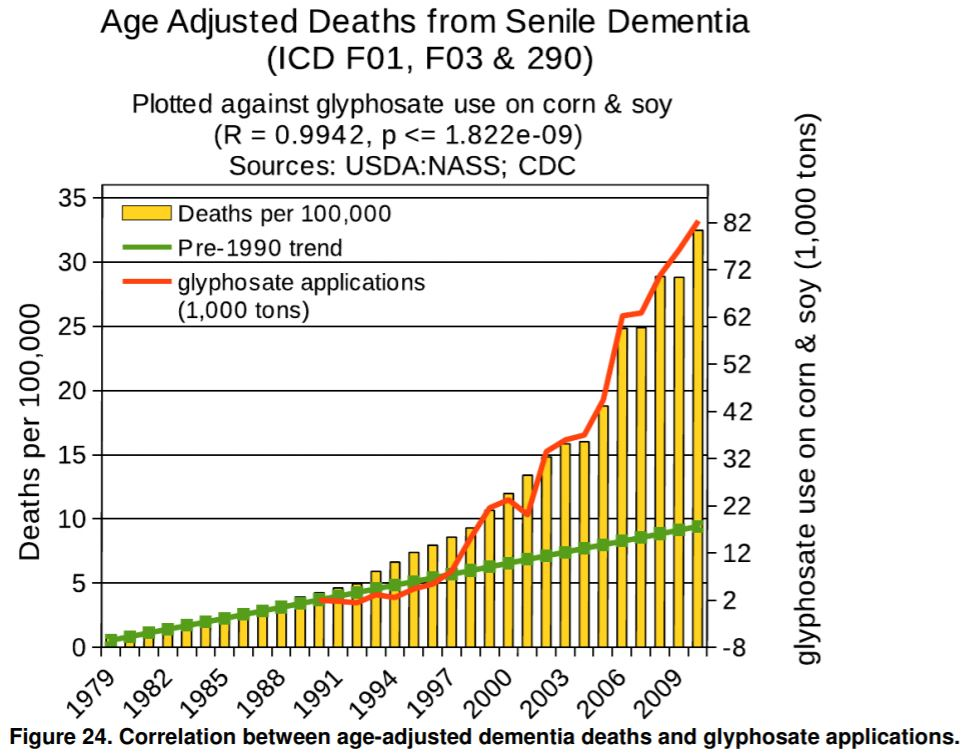
\includegraphics[width = 0.9\textheight]{Swanson-Dementia.JPG}}
%  \only<2>{Glyphosate \textit{vs} Tyroid\\ }
%  \only<2>{ 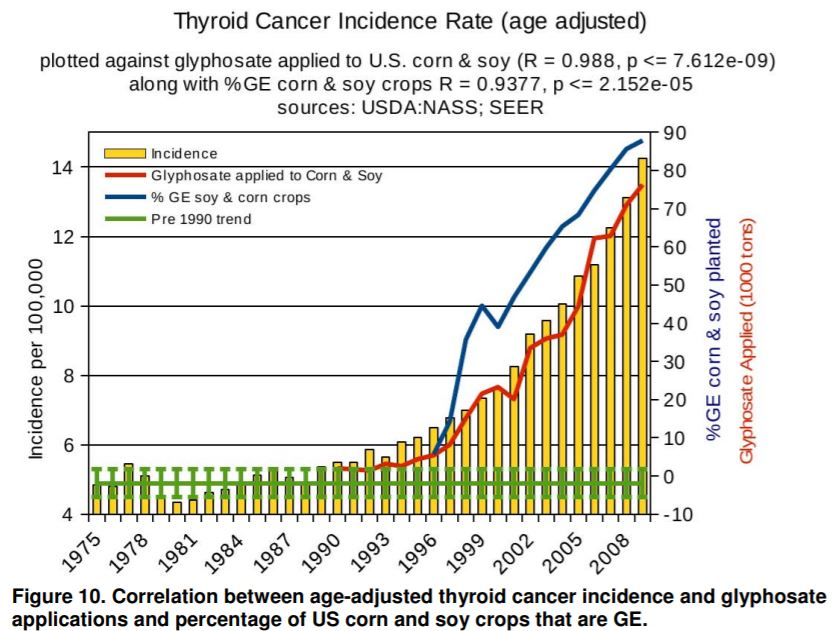
\includegraphics[width = 0.9\textheight]{Swanson-Tyroid.JPG}}
%  \only<3>{Glyphosate \textit{vs} Parkinson\\ }
%  \only<3>{ 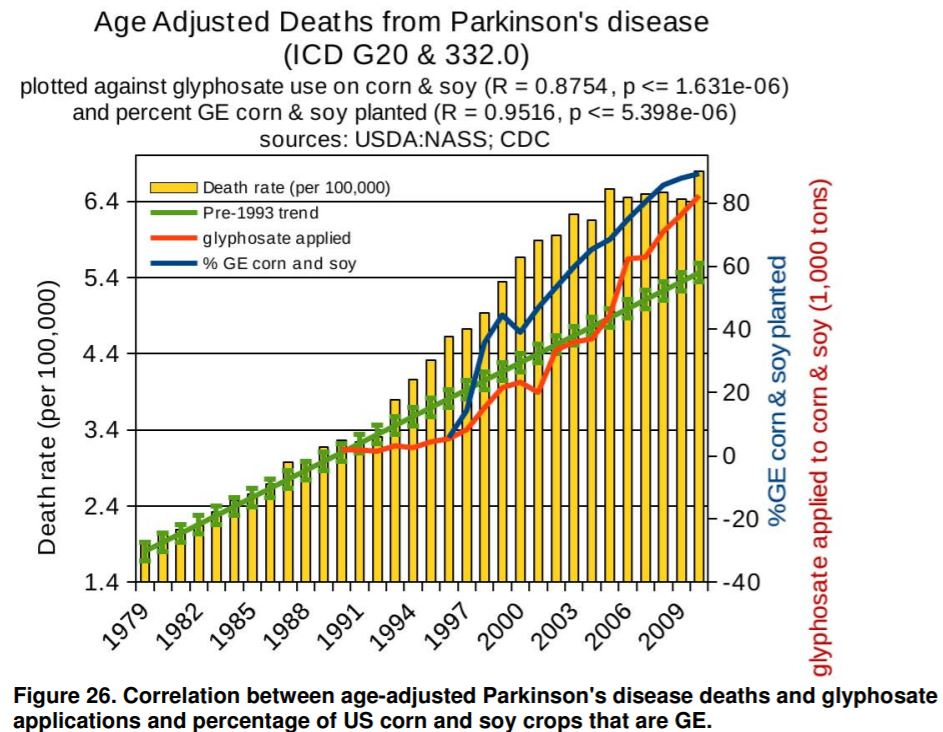
\includegraphics[width = 0.9\textheight]{Swanson-Parkinson.JPG}}
%  \only<4>{Glyphosate \textit{vs} Diabetes\\ }
%  \only<4>{ 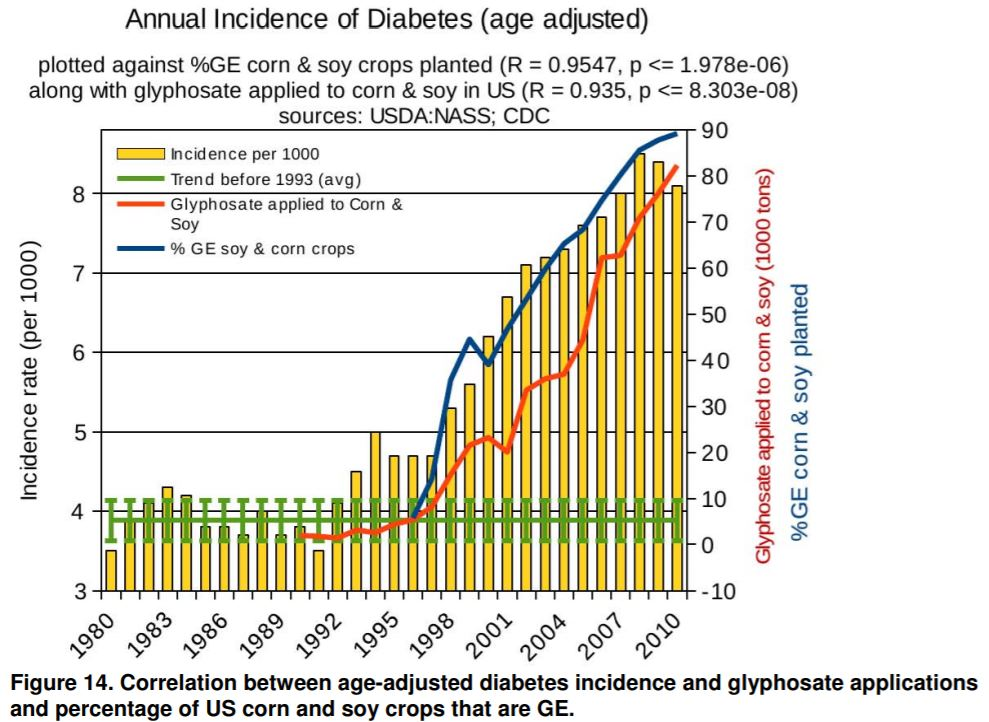
\includegraphics[width = 0.9\textheight]{Swanson-Diabetes.JPG}}
%  \only<5>{Glyphosate \textit{vs} Strokes\\ }
%  \only<5>{ 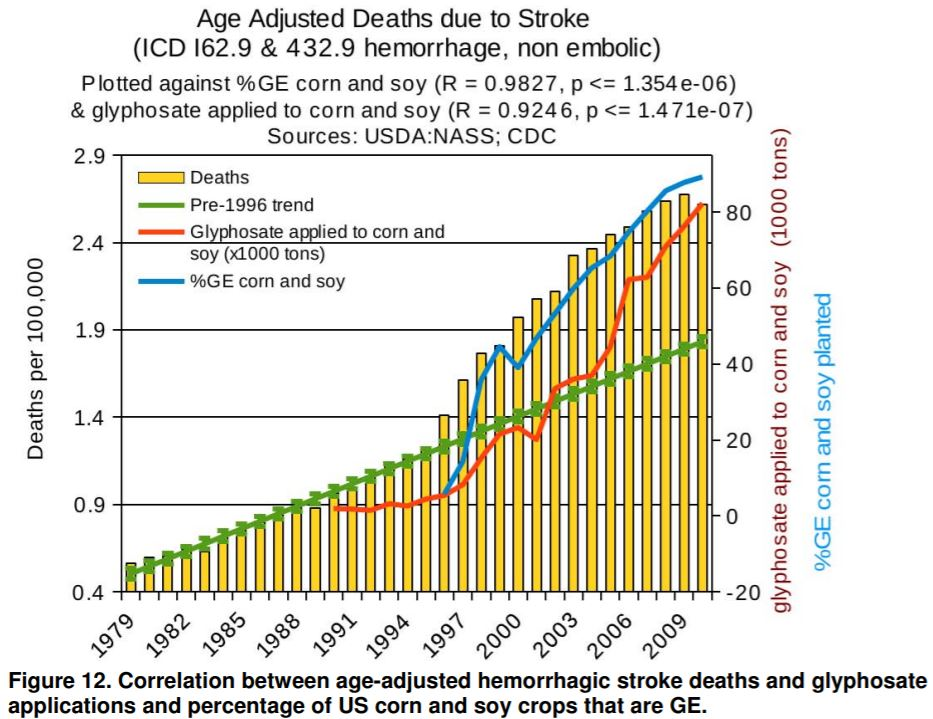
\includegraphics[width = 0.9\textheight]{Swanson-Stroke.JPG}}
%  \only<6>{Glyphosate \textit{vs} Hypertension\\ }
%  \only<6>{ 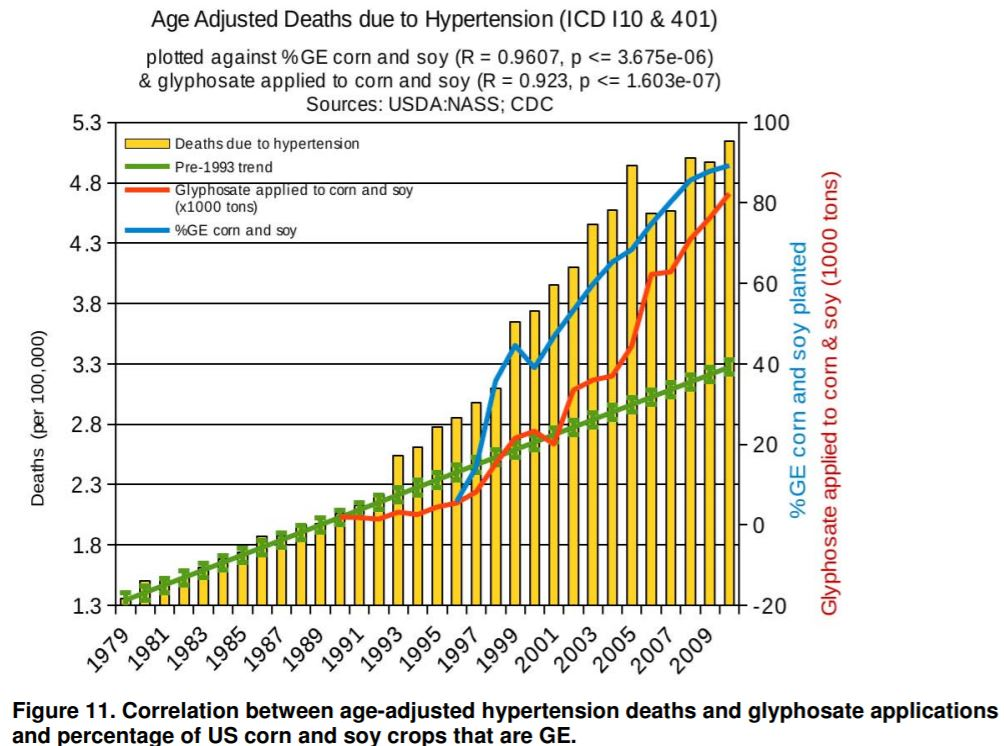
\includegraphics[width = 0.9\textheight]{Swanson-Hypertension.JPG}}
%\end{itemize}
%\end{center}
%\textcolor{gris}{\footnotesize{Source: \href{https://callingbullshit.org/tools/tools_misleading_axes.html}{Calling Bullshit- Original paper Swanson et al. Journal of Organic System (2014)}}}
%\end{frame}


%\begin{frame} % Cover slide
%\frametitle{\textcolor{brique}{[- \textbf{Rule \#3: Use double axes! } -]}}
%Example: Americans United for Life
%\begin{center}
%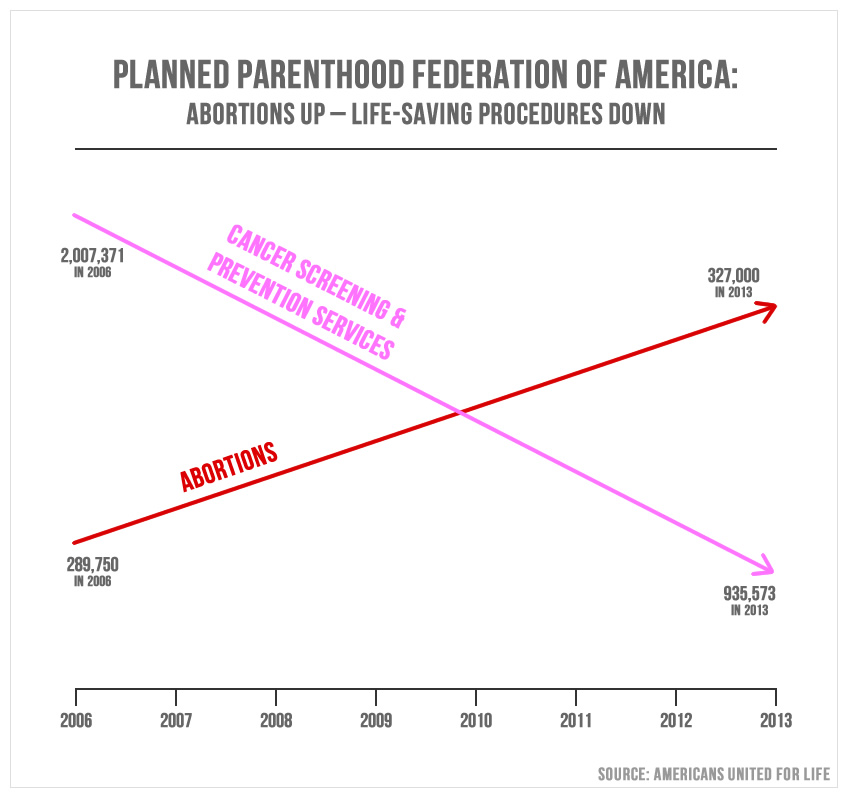
\includegraphics[width = 0.8\textwidth]{AbortionPlanningService.jpg}
%\end{center}
%Do these two curve really cross?  Do they even relate?
%\textcolor{gris}{\footnotesize{Source: \href{https://www.politifact.com/truth-o-meter/statements/2015/oct/01/jason-chaffetz/chart-shown-planned-parenthood-hearing-misleading-/}{ Linda Qiu (Politifac)t}}}
%\end{frame}
%
%\begin{frame} % Cover slide
%\frametitle{\textcolor{brique}{[- \textbf{Rule \#3: Use double axes! } -]}}
%The ``correct'' curves comparing Abortion \& Cancer Prevention Services
%\begin{center}
%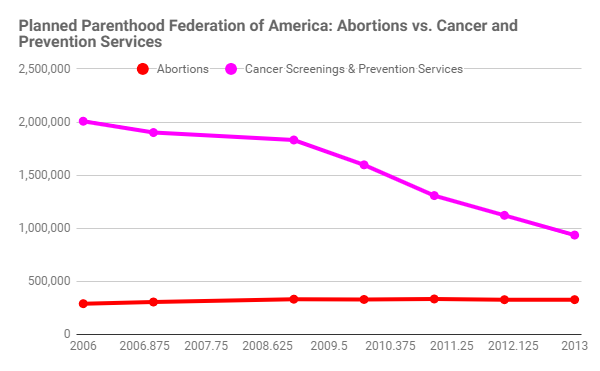
\includegraphics[width = 0.8\textwidth]{AbortionPlanningService2.png}
%\end{center}
%\textcolor{gris}{\footnotesize{Source: \href{https://www.politifact.com/truth-o-meter/statements/2015/oct/01/jason-chaffetz/chart-shown-planned-parenthood-hearing-misleading-/}{ Linda Qiu (Politifact}}}
%
%See also tons of funny examples on \href{http://tylervigen.com/view_correlation?id=233}{\textit{Spurious Correlation} Website}
%\end{frame}

\section{Rule 4}

\begin{frame} % Cover slide
\frametitle{\textcolor{brique}{[-\textbf{Rule \#4: Select your scope }-]}}
% (cherry picking)
\begin{figure}[h]
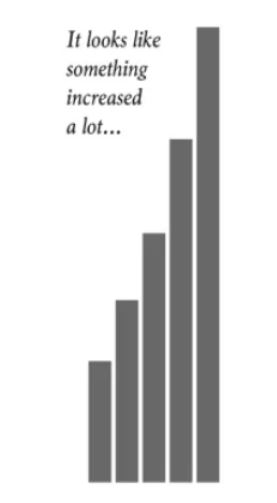
\includegraphics[width = 0.25\textwidth]{LimitedScopePartial.jpg}
\caption{Are you looking at the right thing?}
\end{figure}
\end{frame}

\begin{frame} % Cover slide
\frametitle{\textcolor{brique}{[-\textbf{Rule \#4: Select your scope}-]}}
\begin{figure}[h]
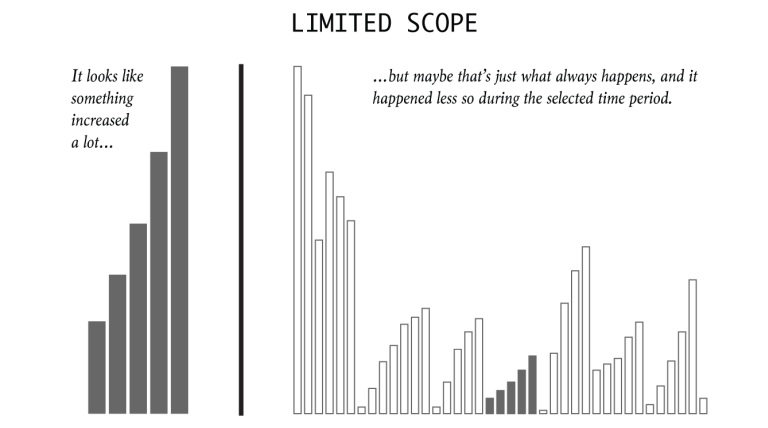
\includegraphics[width = 0.75\textwidth]{Limited-scope.png}
\caption{Cherry picking?}
\end{figure}
\textcolor{gris}{\footnotesize{Source: \href{https://flowingdata.com/2017/02/09/how-to-spot-visualization-lies/}{Flowing data}}}
\end{frame}

%\begin{frame} % Cover slide
%\frametitle{\textcolor{brique}{[-\textbf{Applying Rule \#4: Global Warming}-]}}
%
%\begin{figure}[h]
%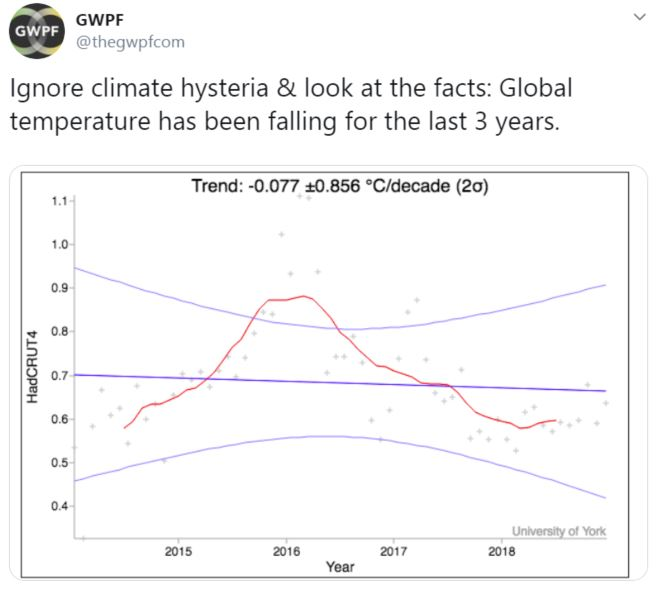
\includegraphics[width = 0.85\textwidth]{NASA-ScopeGlobalWarming0.JPG}
%\caption{Cherry picking!}
%\end{figure}
%\textcolor{gris}{\footnotesize{Source: \href{https://twitter.com/thegwpfcom/status/1153652707049254913}{@thegwpfcom
%, Twitter 2019.}}}
%\end{frame}
%
%\begin{frame} % Cover slide
%\frametitle{\textcolor{brique}{[-\textbf{Applying Rule \#4: Global Warming}-]}}
%
%\begin{figure}[h]
%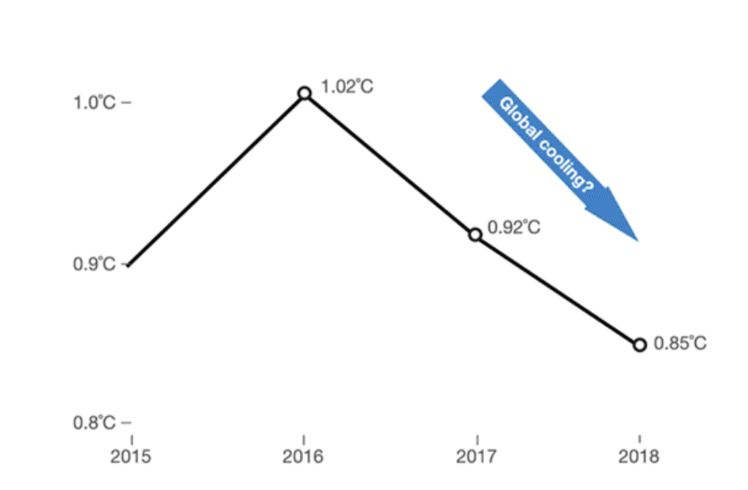
\includegraphics[width = 0.85\textwidth]{NASA-ScopeGlobalWarming1.JPG}
%\caption{Cherry picking!}
%\end{figure}
%\textcolor{gris}{\footnotesize{Source: \href{https://climate.nasa.gov/blog/2893/nope-earth-isnt-cooling/}{"Nope, Earth Isn't Cooling". NASA, 2019.}}}
%\end{frame}
%
%\begin{frame} % Cover slide
%\frametitle{\textcolor{brique}{[-\textbf{Applying Rule \#4: Global Warming}-]}}
%\begin{figure}[h]
%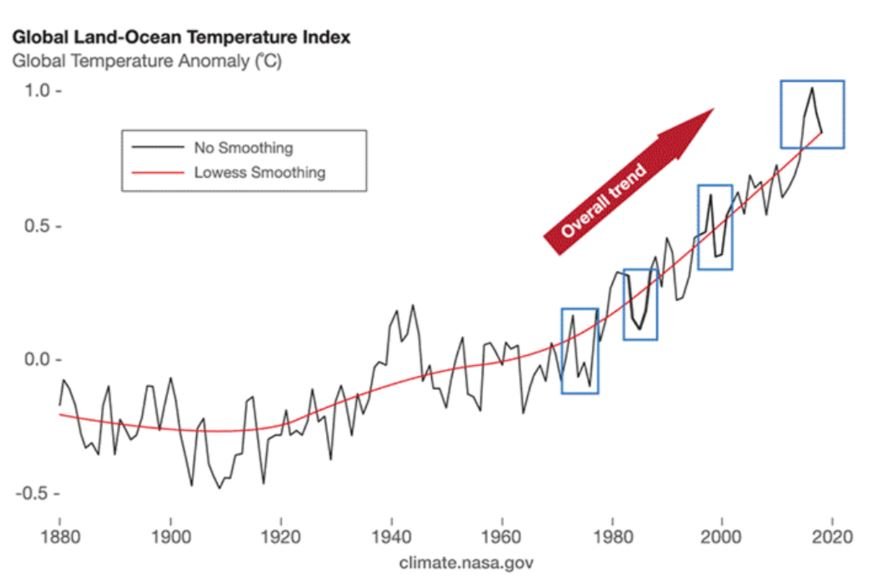
\includegraphics[width = 0.85\textwidth]{NASA-ScopeGlobalWarming2.JPG}
%\caption{Cherry picking!}
%\end{figure}
%\textcolor{gris}{\footnotesize{Source: \href{https://climate.nasa.gov/blog/2893/nope-earth-isnt-cooling/}{"Nope, Earth Isn't Cooling". NASA, 2019.}}}
%
%\end{frame}


\begin{frame} % Cover slide
\frametitle{\textcolor{brique}{[-\textbf{Applying Rule \#4: Brexit !}-]}}
\begin{center}
\begin{itemize}
  \only<1>{ 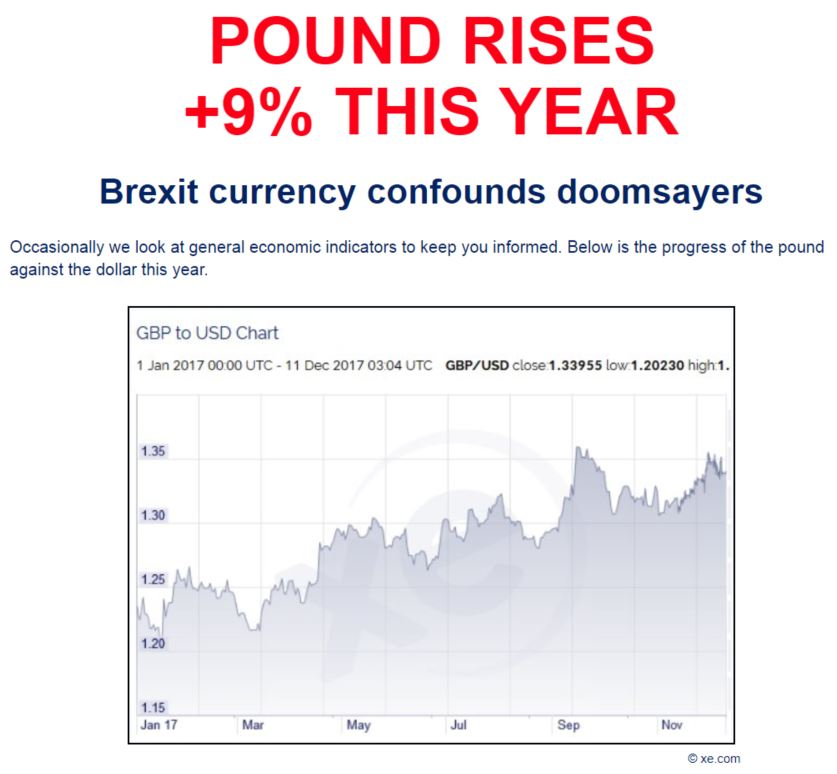
\includegraphics[width = 0.55\textwidth]{GBP-USDRate-Brexiters.JPG} \\ }
  \only<2>{ 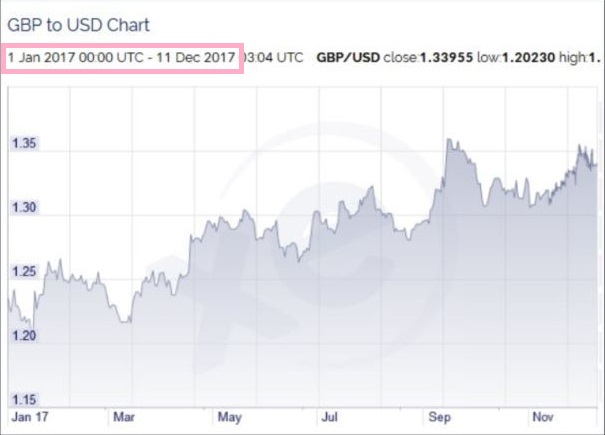
\includegraphics[width = 0.8\textwidth]{GBP-USDRate-Brexiters-Zoom.jpg} \\ }
  \only<1-2>{\textcolor{gris}{\footnotesize{Source: \href{http://facts4eu.org/news_dec_2017.shtml}{Pro-Brexit site( Facts4eu.org)}}} }
  \only<3>{ 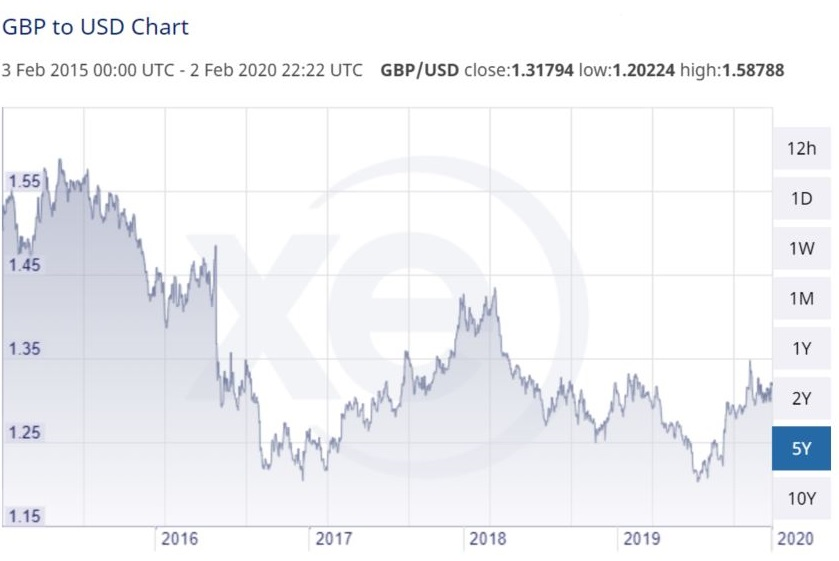
\includegraphics[width = 0.8\textwidth]{GBP-USDRate-5Y.JPG}}
  \only<4>{ 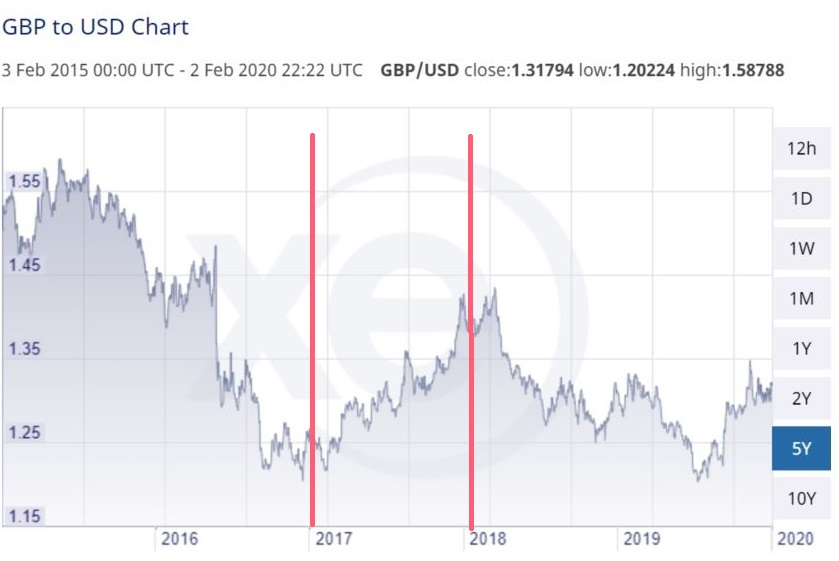
\includegraphics[width = 0.8\textwidth]{GBP-USDRate-5Y-Annotated.jpg}}
  \only<5>{ 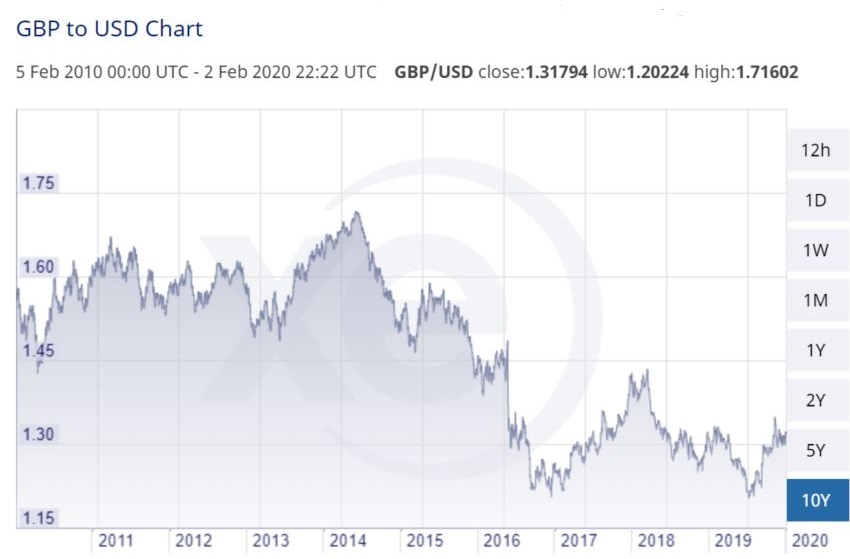
\includegraphics[width = 0.8\textwidth]{GBP-USDRate-10Y.JPG}}
  \only<6>{ 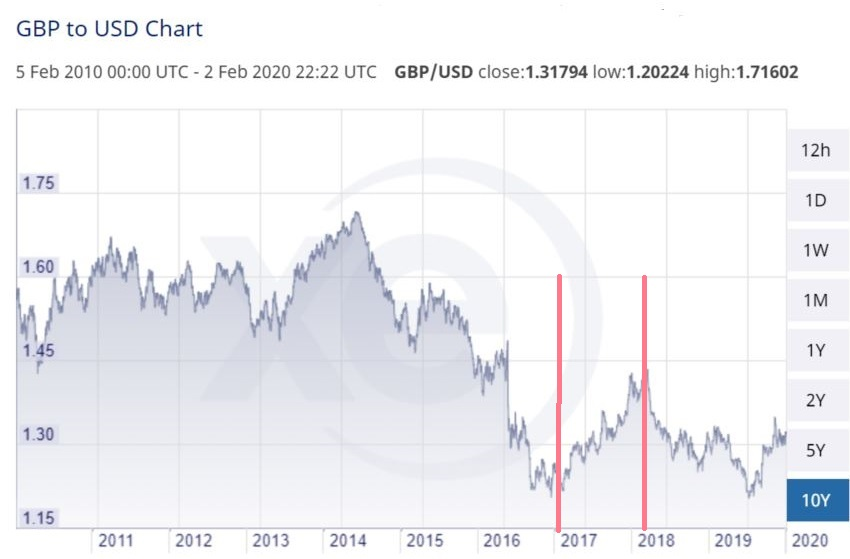
\includegraphics[width = 0.8\textwidth]{GBP-USDRate-10Y-Annotated.jpg}}
\end{itemize}
\end{center}
\end{frame}


\section{Rule 5}

\begin{frame}
\frametitle{\textcolor{brique}{[- \textbf{Rule \#5a: Use 3D } -]}}
 This is \textcolor{brique}{\textbf{very clear}} \\
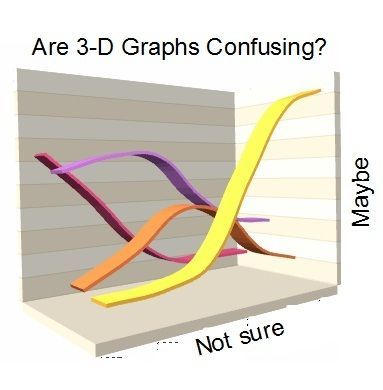
\includegraphics[width = 0.5\textwidth]{WTF-3D-MapS-Confusion.jpg}
\end{frame}

\begin{frame}
\frametitle{\textcolor{brique}{[- \textbf{Rule \#5a: Use 3D Bars} -]}}
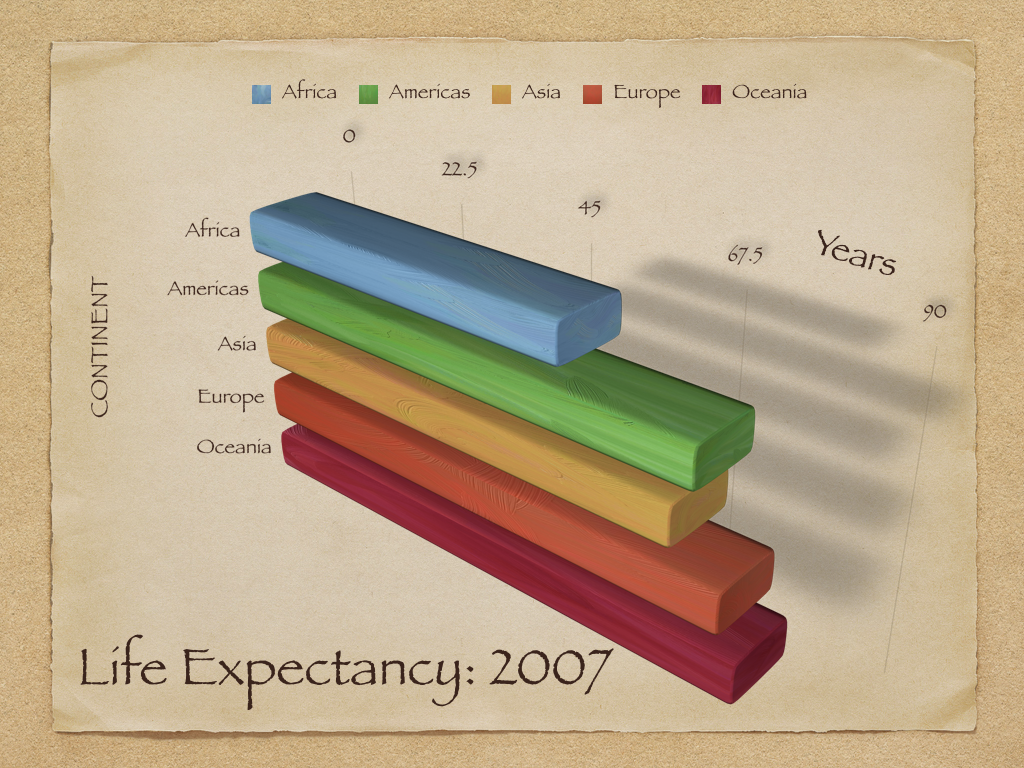
\includegraphics[width = 0.6\textwidth]{Heally-ch-01-chartjunk-life-expectancy.png}\\
\textcolor{gris}{\footnotesize{Source \cite{Healy2019}}}
\end{frame}

\begin{frame}
\frametitle{\textcolor{brique}{[- \textbf{Rule \#5a: Use 3D } -]}}
 This is \textcolor{brique}{\textbf{Bananas}} \\
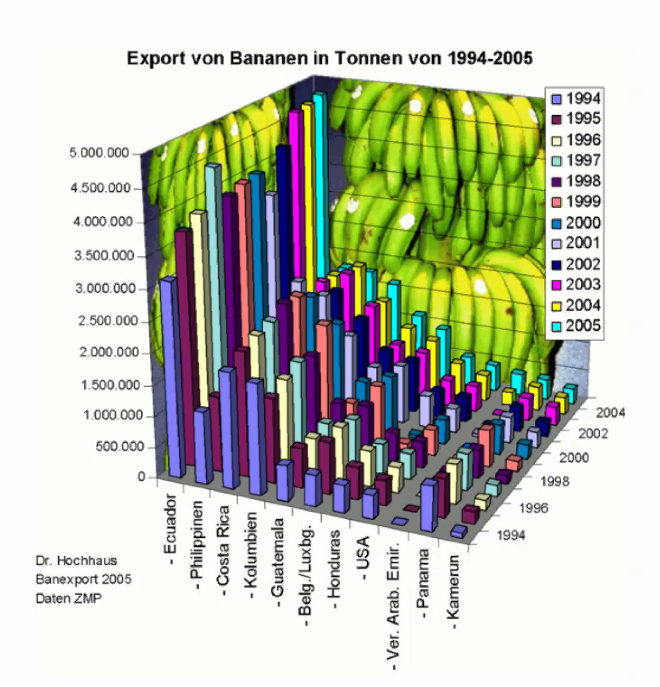
\includegraphics[width = 0.5\textwidth]{3DbarsBananas.png}
\end{frame}



\begin{frame}
\frametitle{\textcolor{brique}{[- \textbf{Rule \#5a: Use 3D } -]}}
Monthly expenses...  \\
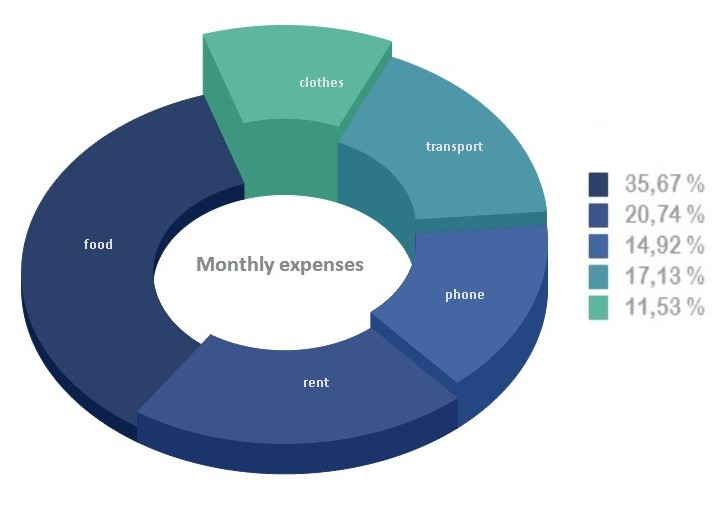
\includegraphics[width = 0.7\textwidth]{3D-Pie_ChartN.jpg}
\end{frame}


\begin{frame}
\frametitle{\textcolor{brique}{[- \textbf{Rule \#5b: Use 3D pie charts} -]}}
Do as \textbf{Steve Jobs}!
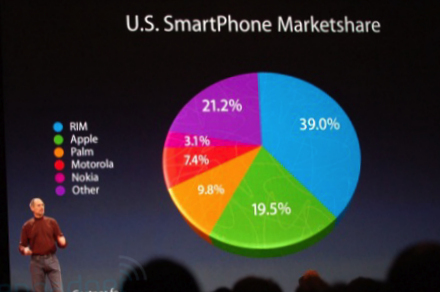
\includegraphics[width = 0.7\textwidth]{SteveJob.jpg} \\
\textcolor{gris}{\footnotesize{Source (Macworld 2008 keynote lecture}}
\end{frame}

\begin{frame}
\frametitle{\textcolor{brique}{[- \textbf{Rule \#5b: Use 3D pie charts} -]}}
Do as Steve Jobs!

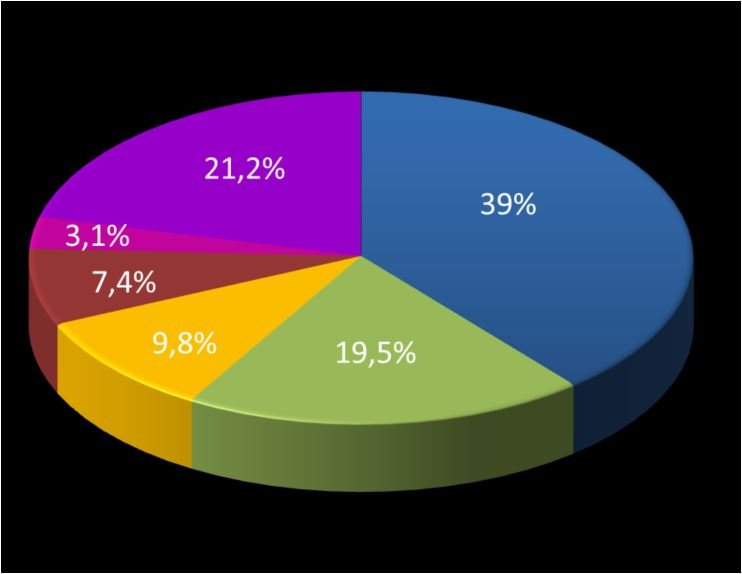
\includegraphics[width = 0.6\textwidth]{SteveJobExcell.jpg}

\end{frame}

\begin{frame}
\frametitle{\textcolor{brique}{[- \textbf{Rule \#5b: Use 3D pie charts} -]}}
Do as Steve Jobs!

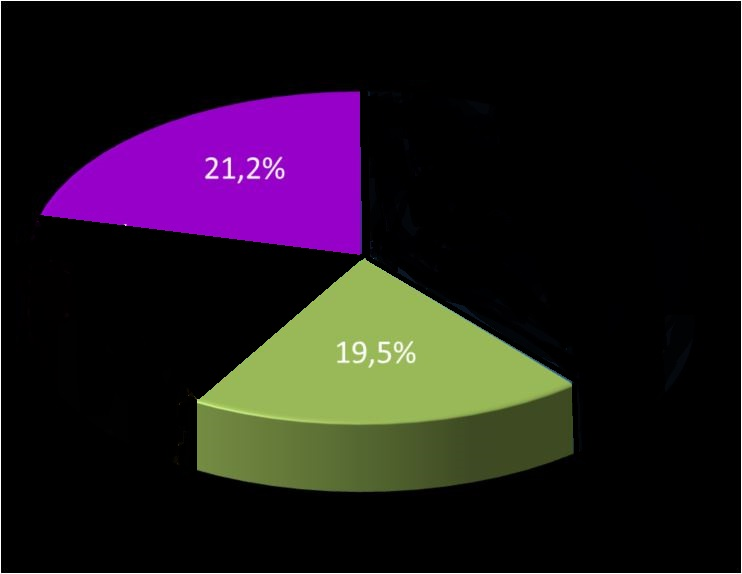
\includegraphics[width = 0.6\textwidth]{SteveJobExcell2.jpg}
%\textcolor{gris}{\footnotesize{Source (Macworld 2008 keynote lecture}}
\end{frame}

\begin{frame}
\frametitle{\textcolor{brique}{[- \textbf{Rule \#5b: Use 3D pie charts} -]}}
Do as Steve Jobs: \textbf{Lie!}

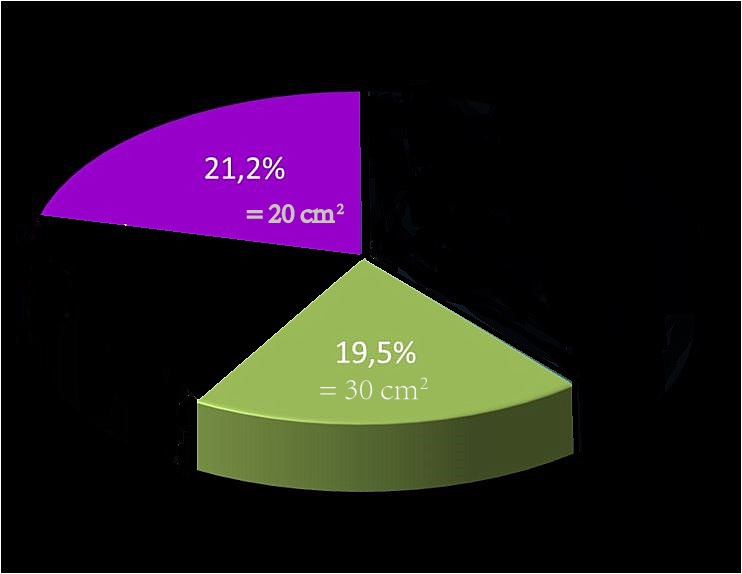
\includegraphics[width = 0.6\textwidth]{SteveJobExcell3.jpg}
%\textcolor{gris}{\footnotesize{Source (Macworld 2008 keynote lecture}}
\end{frame}

%
%\begin{frame} % Cover slide
%\frametitle{\textcolor{brique}{[- \textbf{Rule \#5-bis: Use pie charts  } -]}}
%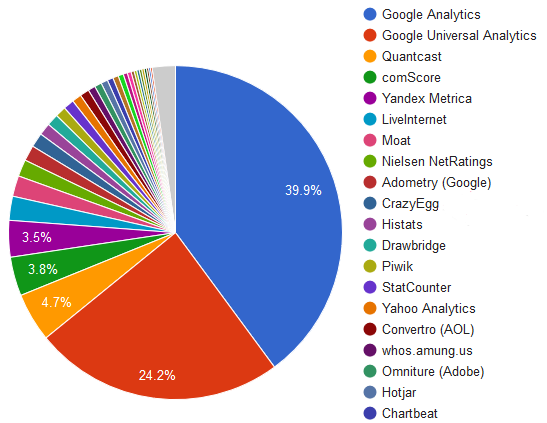
\includegraphics[width =0.6\textwidth]{WTF-UnicornPie-Morethan7Segments.png} \\
%\textcolor{gris}{\footnotesize{From \href{http://viz.wtf/}{WTF Visualisations}}}
%\end{frame}


\begin{frame} % Cover slide
\frametitle{\textcolor{brique}{[- \textbf{A note on pie charts  } -]}}
\begin{center}
\begin{itemize}
 % \only<1>{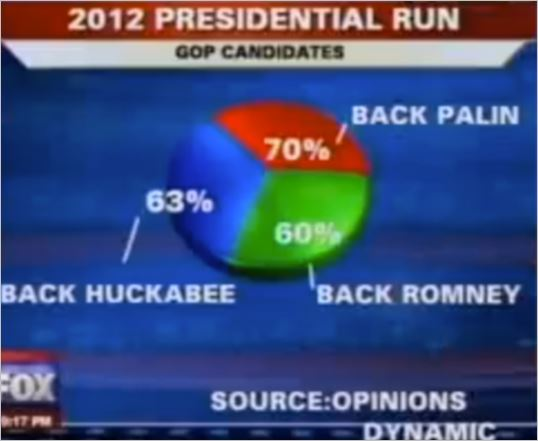
\includegraphics[width =0.7\textwidth]{FoxPieChart.jpg} \\}
%  \only<1>{\textcolor{gris}{\footnotesize{From \href{https://www.nbcchicago.com/news/local/FOX-News-Chart-Fails-Math-73711092.html}{FOX News}}}}
  \only<1>{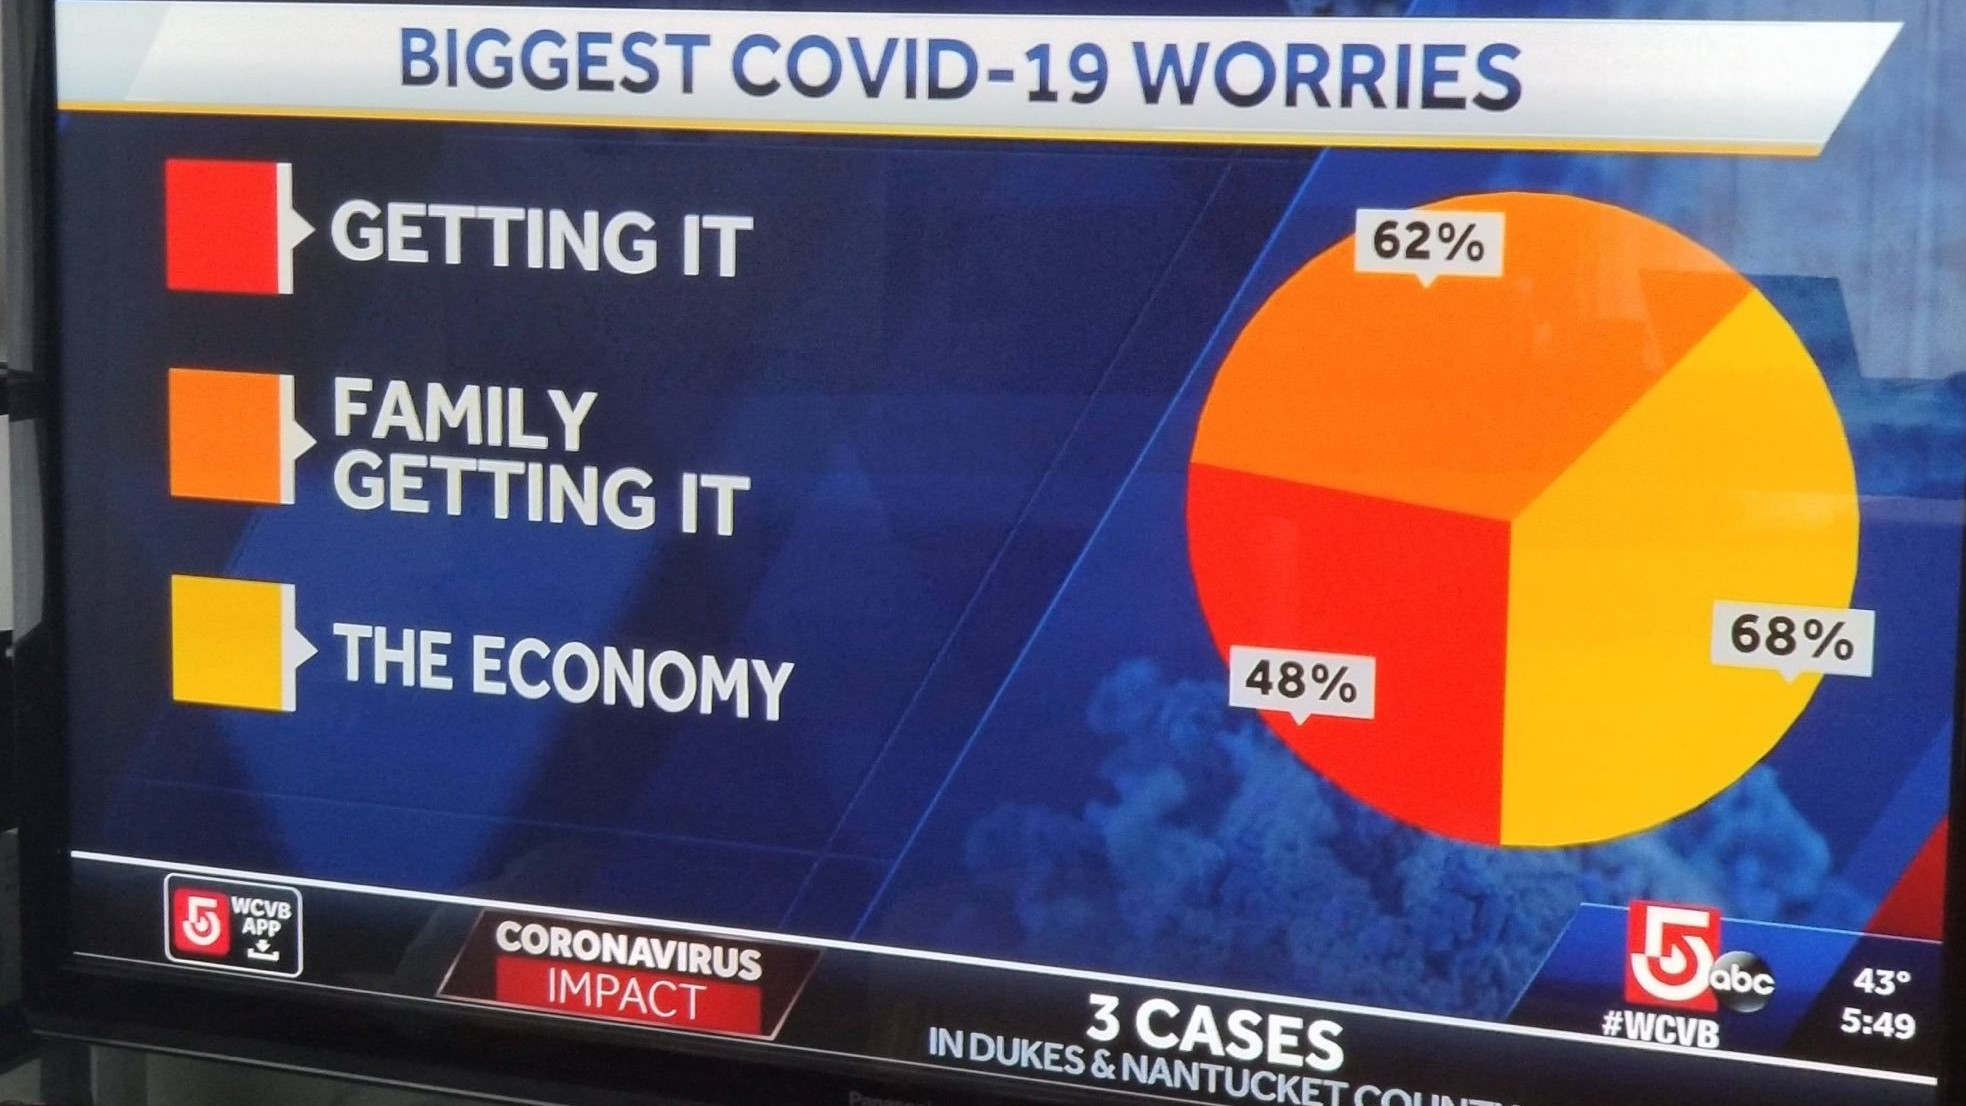
\includegraphics[width =0.8\textwidth]{PieChartLiesCovid19.jpg} \\}
  \only<1>{\textcolor{gris}{\footnotesize{From \href{https://twitter.com/meme_ec/status/1243956187378434049}{WCVB (via Twitter) }}}}
\end{itemize}
\end{center}
\end{frame}


%\begin{frame} % Cover slide
%\frametitle{\textcolor{brique}{[- \textbf{A note on pie charts  } -]}}
%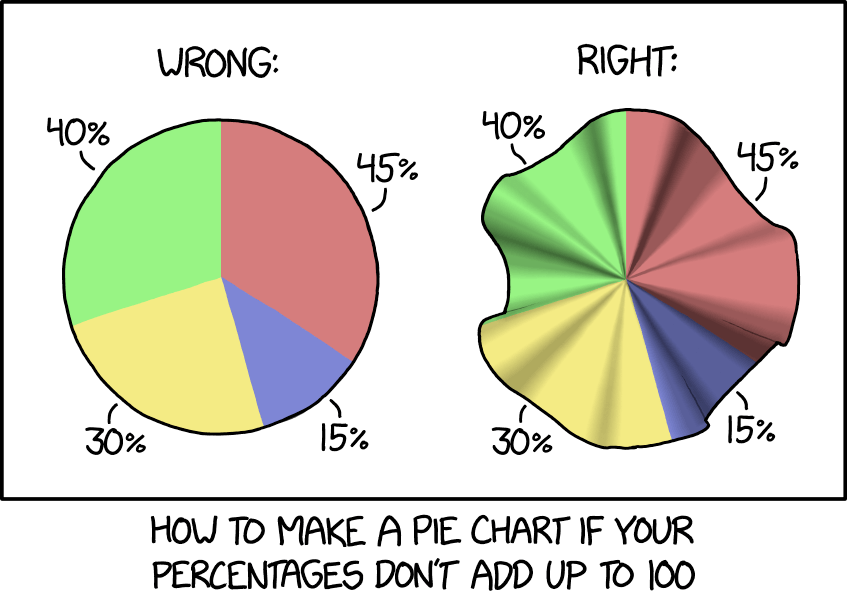
\includegraphics[width =0.7\textwidth]{XKCD-pie_charts_2x.png} \\
%\textcolor{gris}{\footnotesize{From \href{https://xkcd.com/2031/}{XKCD}}}
%\end{frame}

%\begin{frame} % Cover slide
%\frametitle{\textcolor{brique}{[- So you really want to do a \sout{Pyramid} Pie chart? -]}}
%
%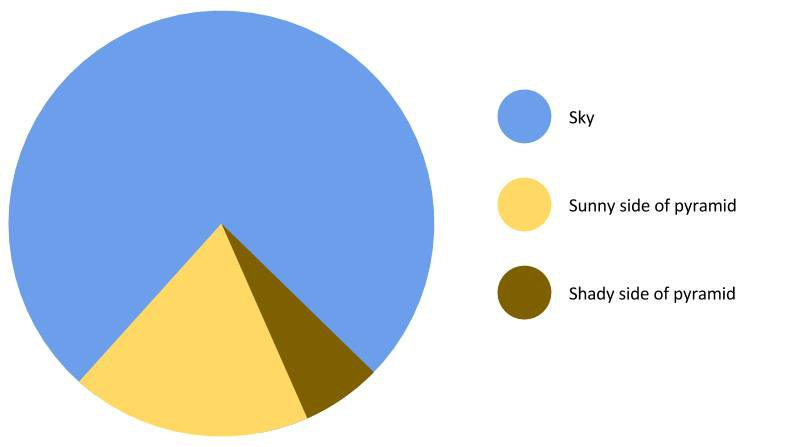
\includegraphics[width =0.8\textwidth]{PiePyramid.jpg}
%
%\textcolor{gris}{\footnotesize{Source :\href{http://www.rebeccabarter.com/blog/2015-07-23-pie/}{Rebecca Barter}}}
%\end{frame}
%
%\begin{frame} % Cover slide
%\frametitle{\textcolor{brique}{[So you really want to do a pie chart? -]}}
%Do it right (unlike your software!)
%\begin{tabular}{lcr}
%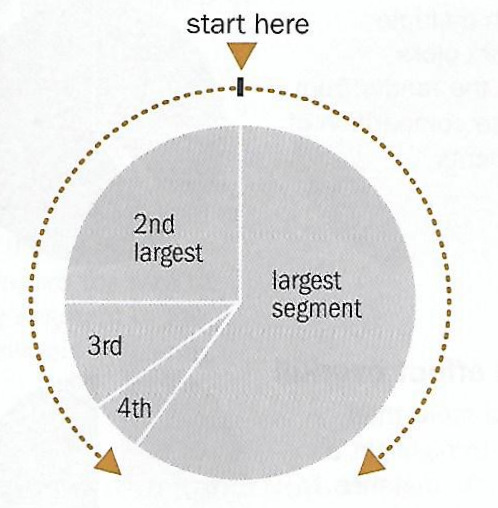
\includegraphics[width =0.4\textwidth]{Dong-WayTodoaPie.jpg}
%\end{tabular}
%from \cite{wong2010}
%\end{frame}


\section{Rule 6}

\begin{frame} % Cover slide
\frametitle{\textcolor{brique}{[- \textbf{Rule \#6: Use several pie charts  } -]}}
\begin{center}
\begin{itemize}
  \only<1-2>{ 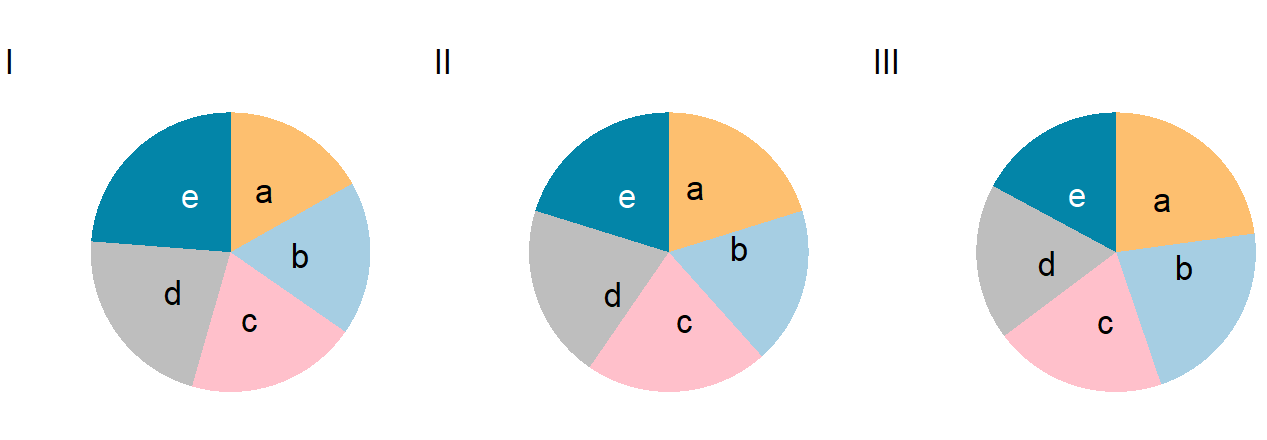
\includegraphics[width =0.9\textwidth]{Compare3Pies.png} }
  \only<2>{ \hfill \textcolor{brique}{ \textbf{Poll}} }
  \only<3>{ 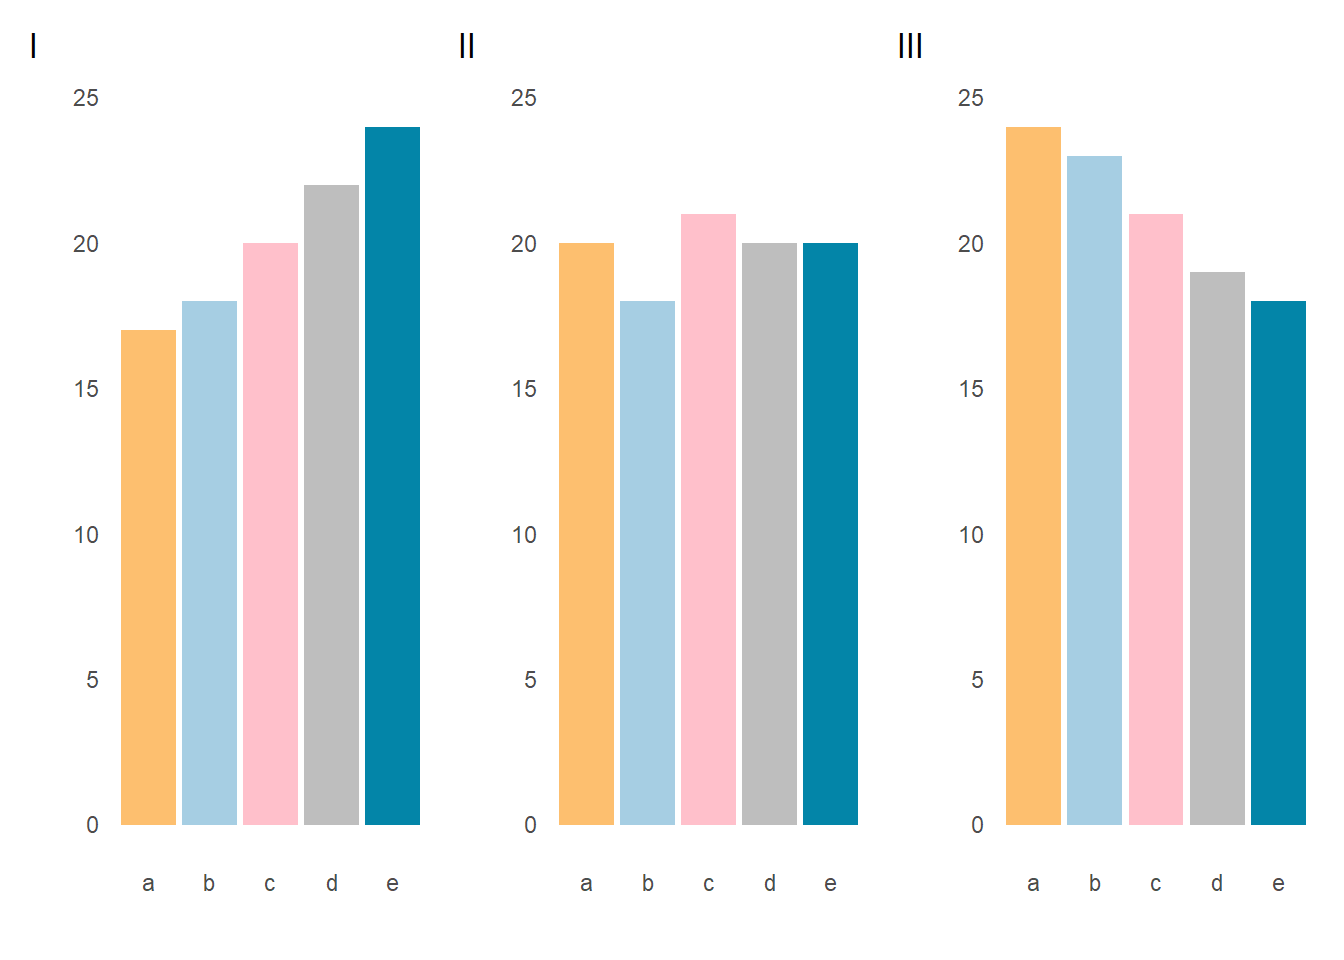
\includegraphics[width =0.65\textwidth]{Compare3BarsV.png} \\}
  \only<4>{ 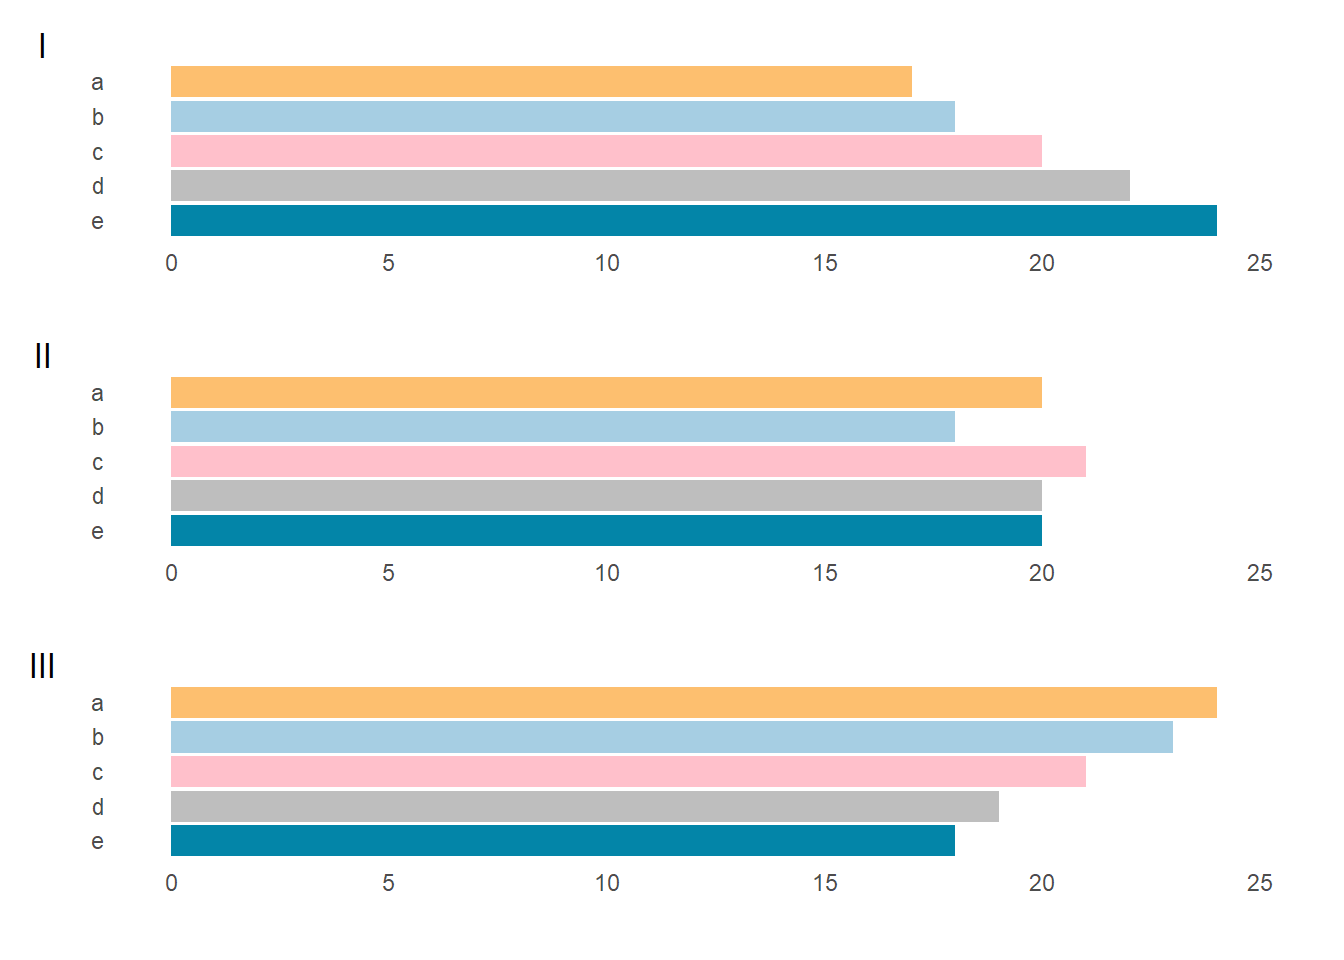
\includegraphics[width =0.65\textwidth]{Compare3BarsH.png} \\}
  \only<5>{ 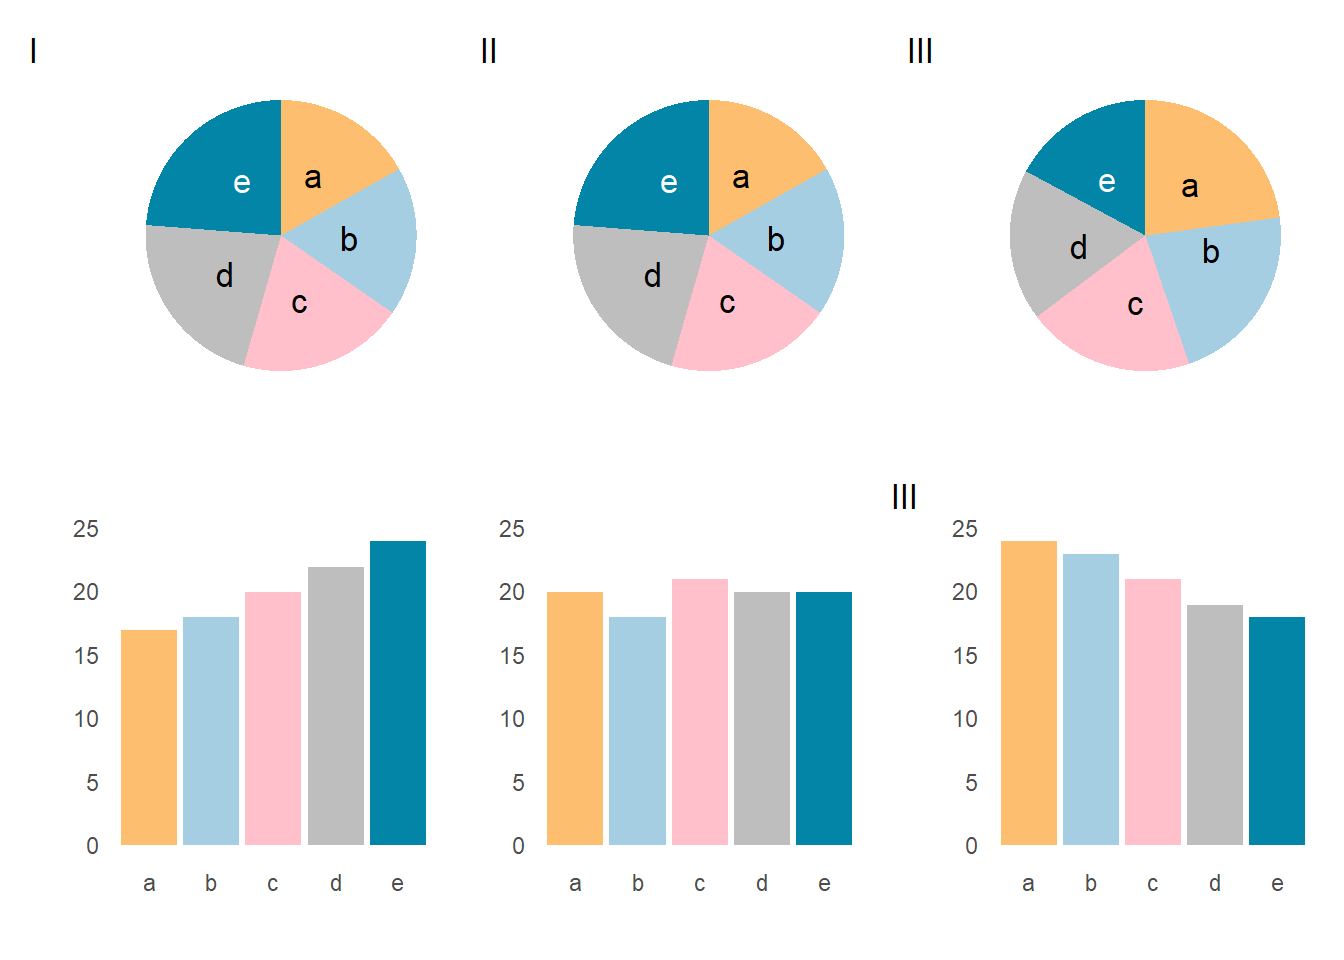
\includegraphics[width =0.65\textwidth]{Compare3PiesBars.png} \\}
  \only<6>{ 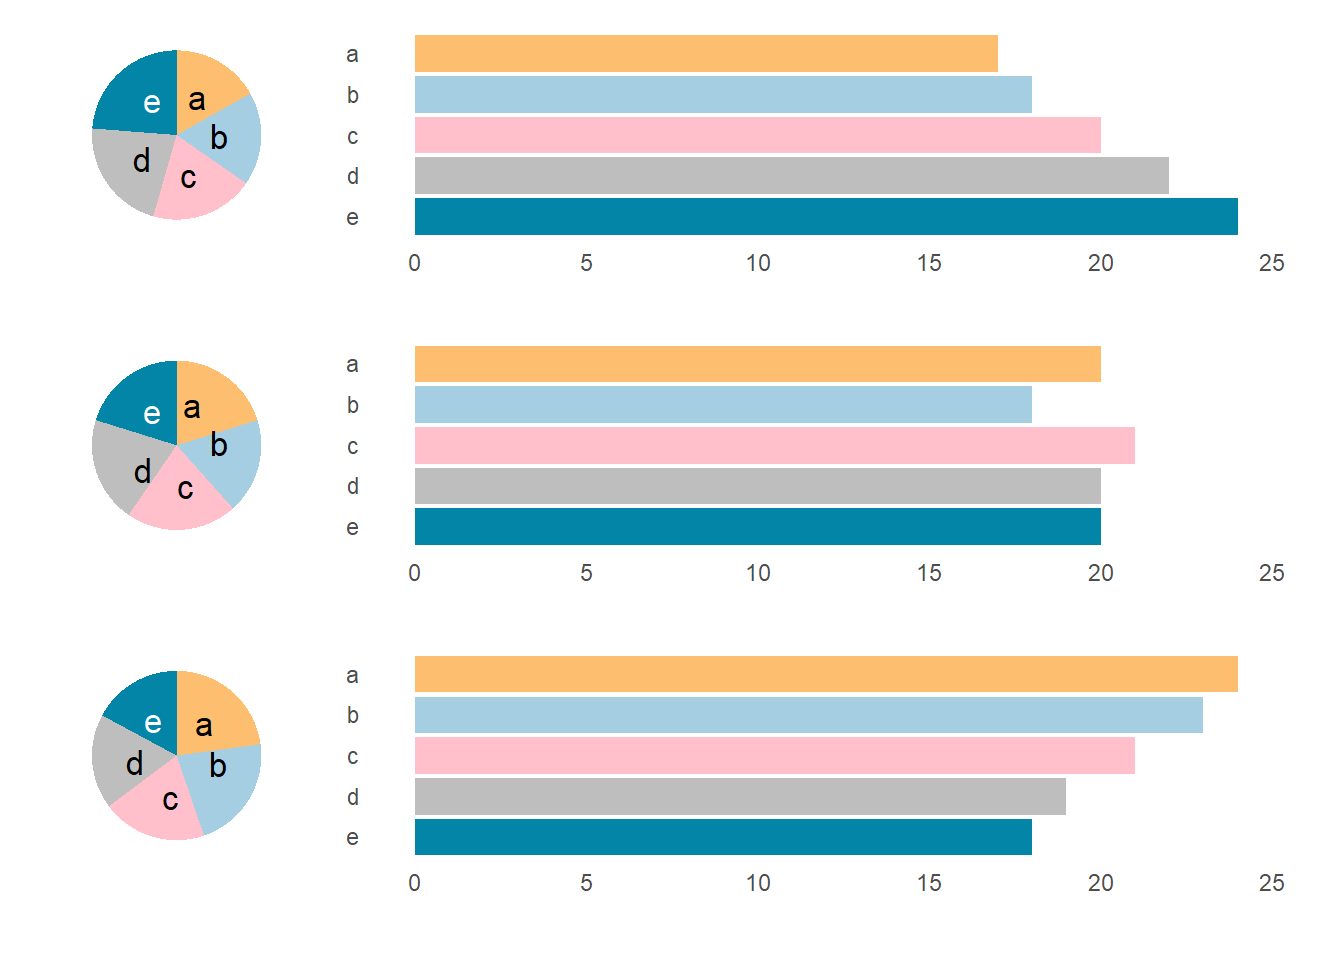
\includegraphics[width =0.65\textwidth]{Compare3PiesBarsH.png} \\}
  \only<1-6>{ \vfill \textcolor{gris}{\footnotesize{Inspired by \href{https://www.data-to-viz.com/caveat/pie.html}{data-to-viz.com}}} }
\end{itemize}
\end{center}
\end{frame}


\begin{frame}
\frametitle{\textcolor{brique}{[- \textbf{Rule \#6: Use several pie charts} -]}}

Refugees to US map by state and nationality (Oct. 2016 - Jan. 2017)
\begin{center}
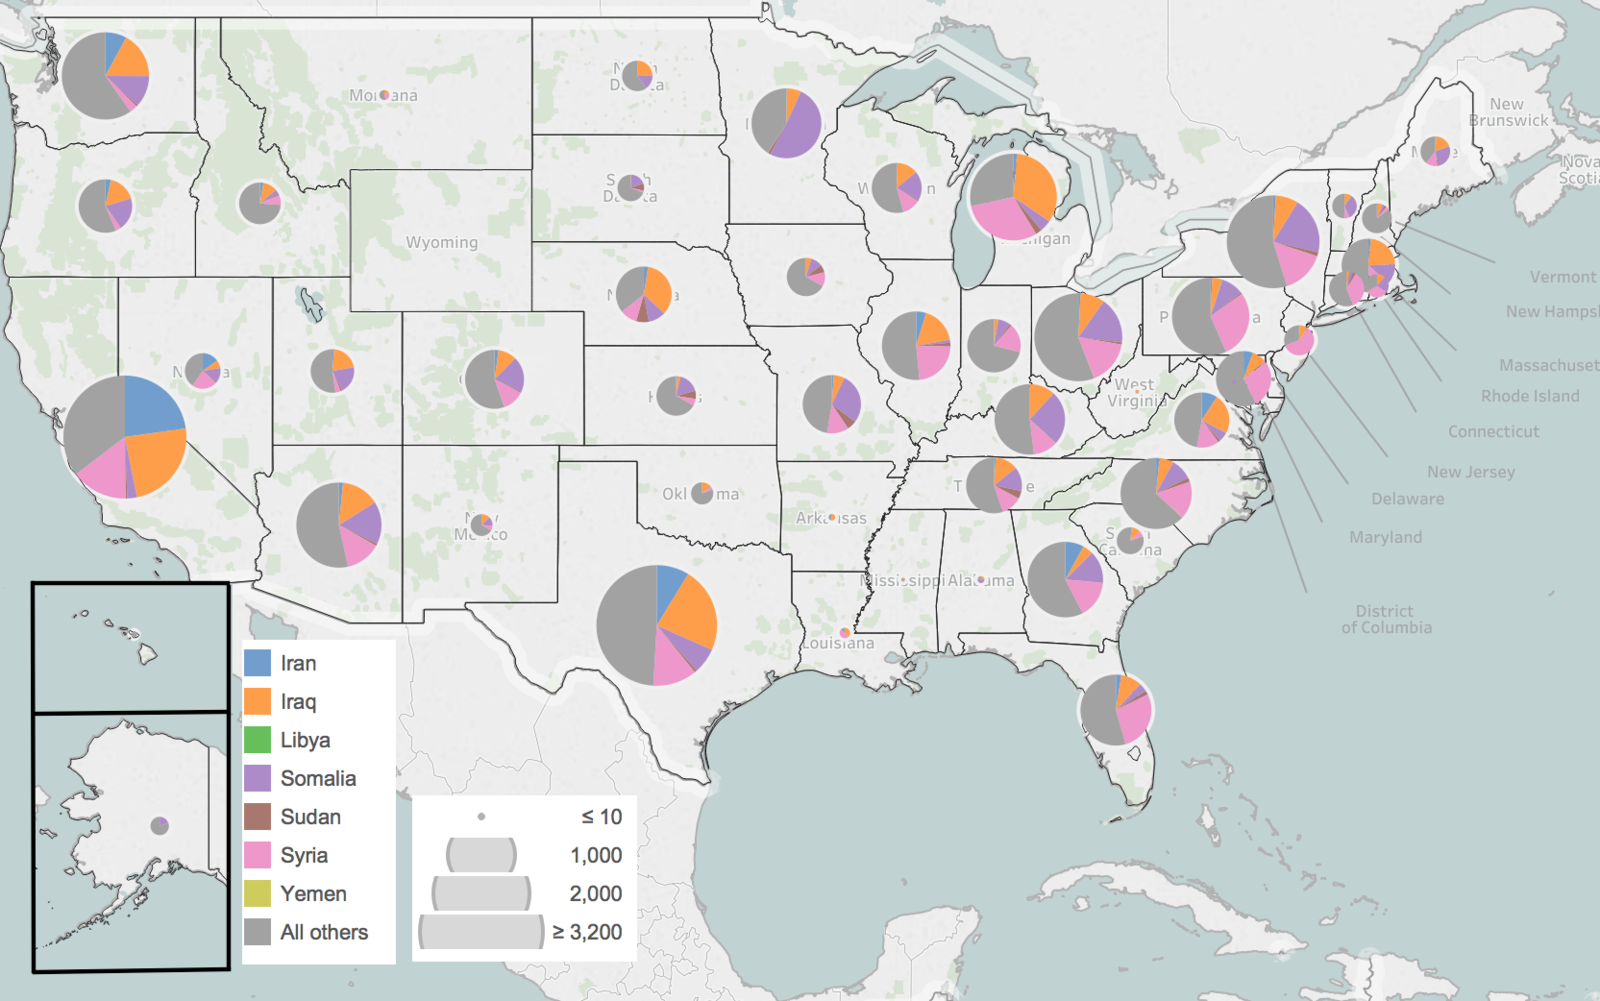
\includegraphics[width = 0.7\textwidth]{PiesOnMaps-Wikimedia.png}\\
\end{center}
\textcolor{gris}{\footnotesize{Source \href{https://commons.wikimedia.org/wiki/File:Refugees_to_US_map_by_state_and_nationality_in_Executive_Order_13769,_for_Oct_1,_2016_to_Jan_31,_2017.png}{Wikimedia}}}
\end{frame}


\section{Rule 7}


\begin{frame} % Cover slide
\frametitle{\textcolor{brique}{[- \textbf{Rule \#7: Use areas  } -]}}
\begin{center}
\begin{itemize}
  \only<1>{Maximize your intakes: One big or two smaller pizzas?}
  \only<1>{ 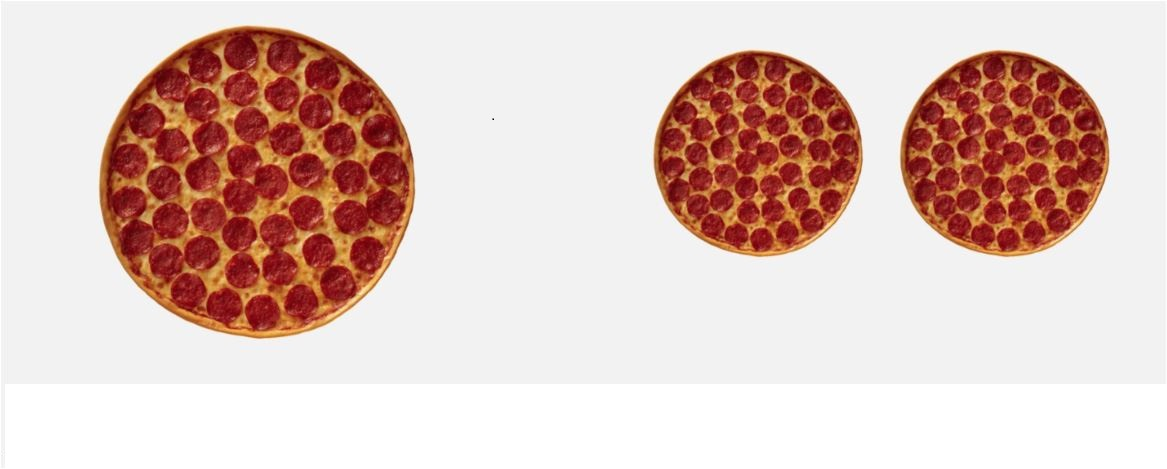
\includegraphics[width =0.95\textwidth]{PizzaCirclesNolegend.jpg} }
  \only<2>{ One big $ >$  two smaller pizzas! \\}
  \only<2>{ 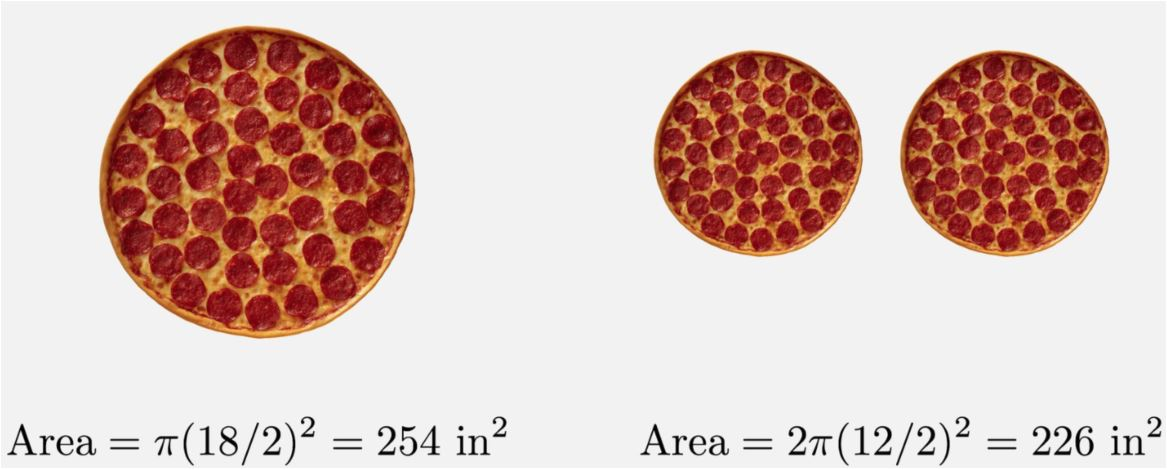
\includegraphics[width =0.95\textwidth]{PizzaCircleslegend.jpg} \\}
  \only<3>{ 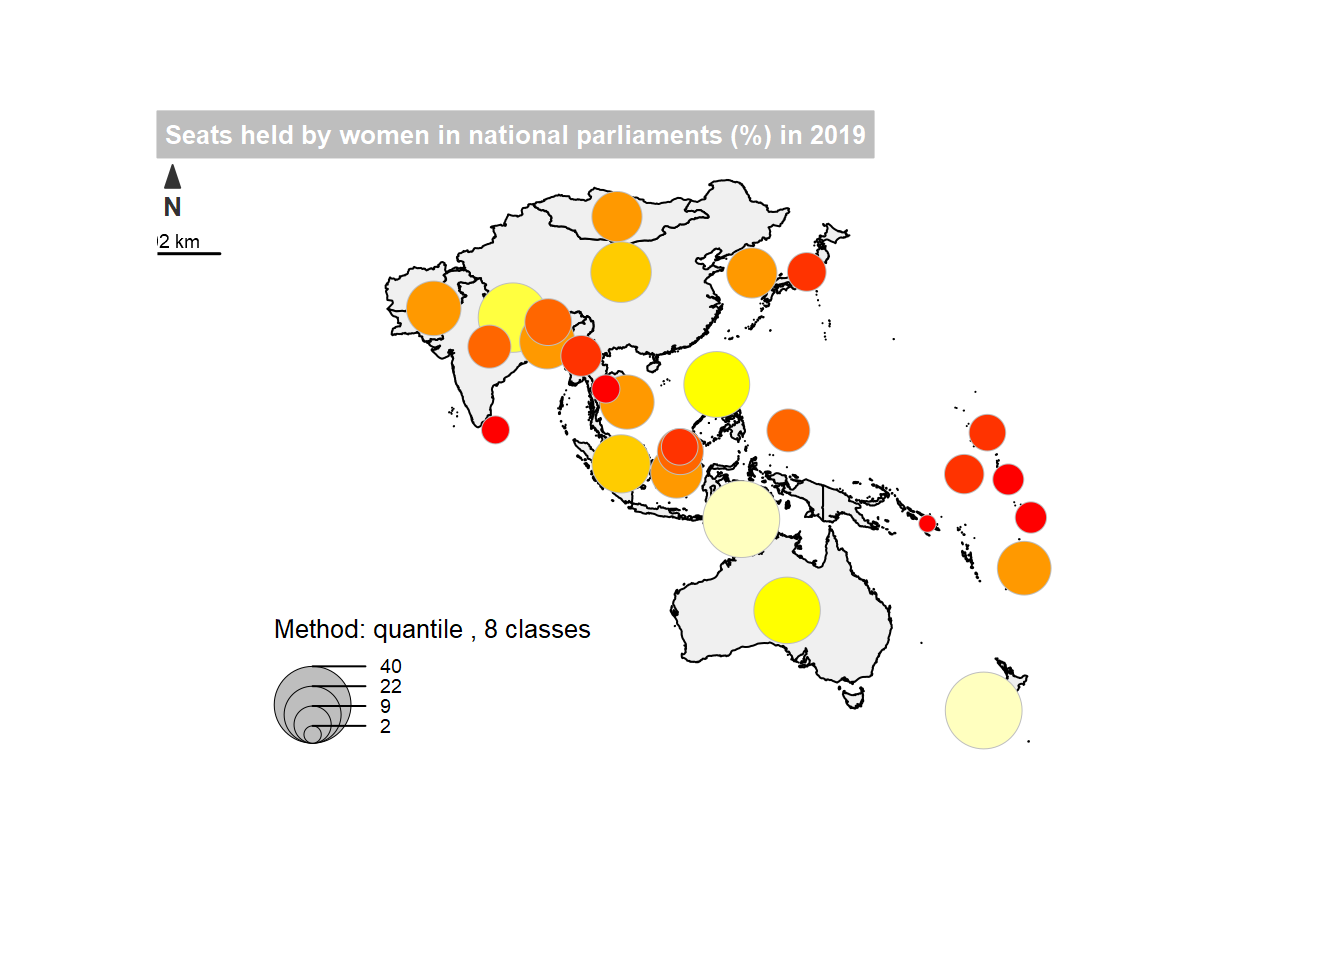
\includegraphics[width =0.9\textwidth]{BubbleMap.png} }
  \only<1-2>{\textcolor{gris}{\footnotesize{Source: \href{https://twitter.com/fermatslibrary/status/1082273172114862083}{Fermat's library}}} \hfill \textcolor{brique}{\textbf{Poll}}  }

\end{itemize}
\end{center}
\end{frame}

%% Squares

\begin{frame} % Cover slide
\frametitle{\textcolor{brique}{[- \textbf{Rule \#7b: Use areas  } -]}}
\begin{center}
\begin{itemize}
  \only<1-2>{If 100\% of  the US prisoners are represented by the big green square...what is the percentage for each group ?}
  \only<1>{ 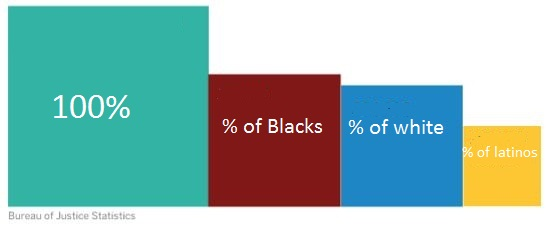
\includegraphics[width =0.9\textwidth]{PrisonniersUSABlind-EN.jpg} }
  \only<2>{ 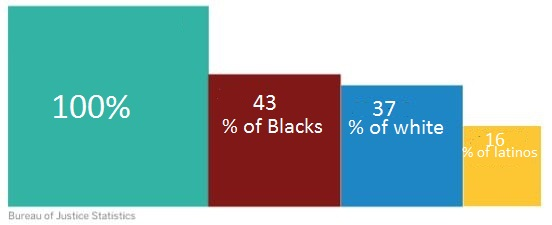
\includegraphics[width =0.9\textwidth]{PrisonniersUSA-EN.jpg} \\ }
  \only<3>{ 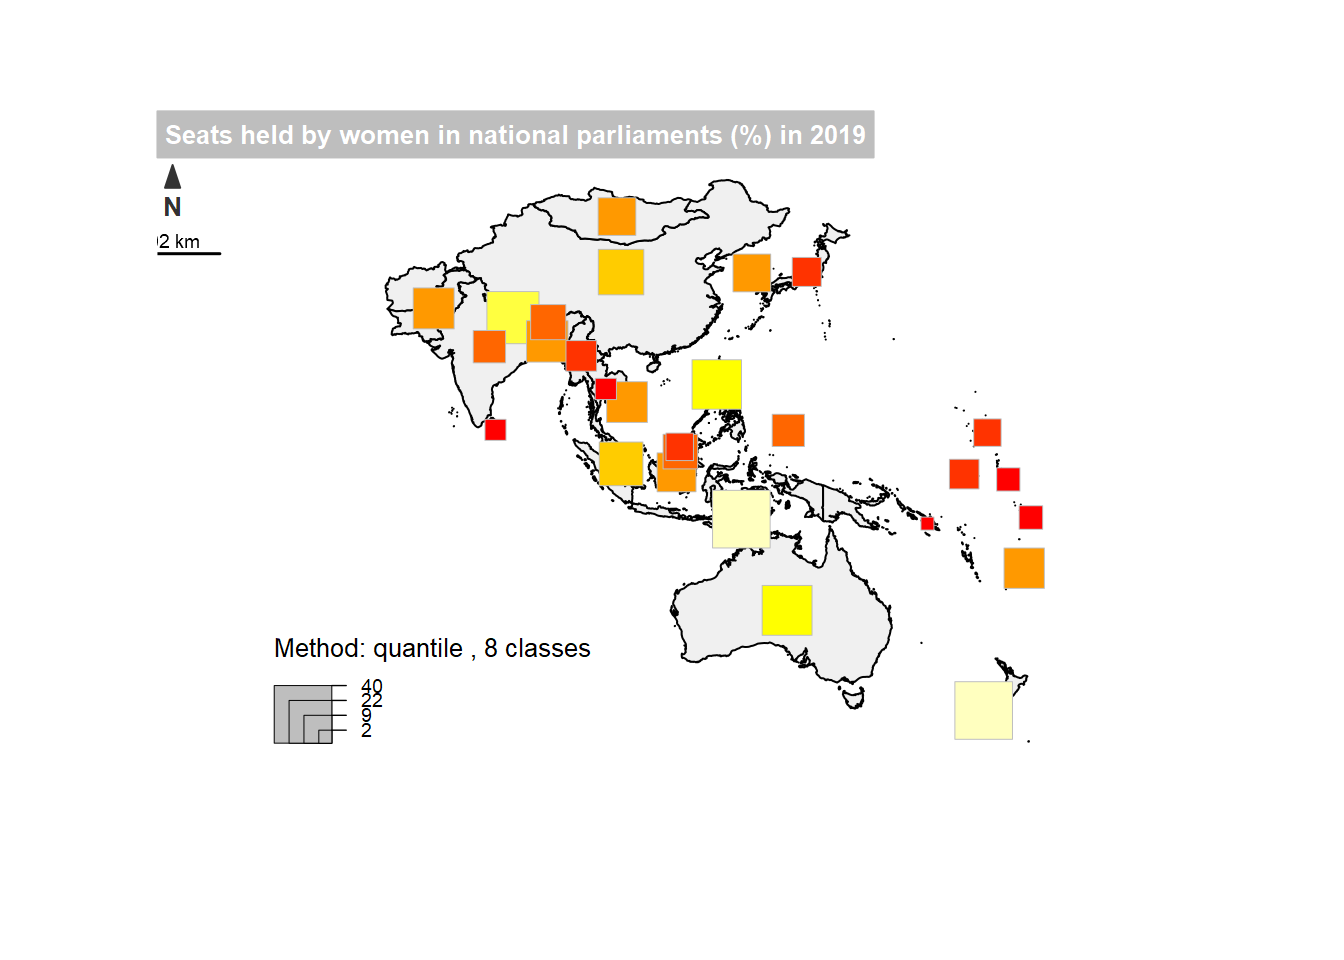
\includegraphics[width =0.9\textwidth]{BubbleMapSquares.png} }
  \only<1-2>{\textcolor{gris}{\footnotesize{Source: Ethic composition of prisoners in Jail in 2008 in the USA.(Le Monde 5/12/2014)}}  \hfill \textcolor{brique}{\textbf{Poll}}  }
\end{itemize}
\end{center}
\end{frame}



\section{Rule 8}


\begin{frame} % Cover slide
\frametitle{\textcolor{brique}{[- \textbf{Rule \#8: Use [unaligned] bars} -]}}
\begin{center}
\begin{itemize}
  \only<1-2>{Bar A or B: Which one is the tallest? \\ }
  \only<1>{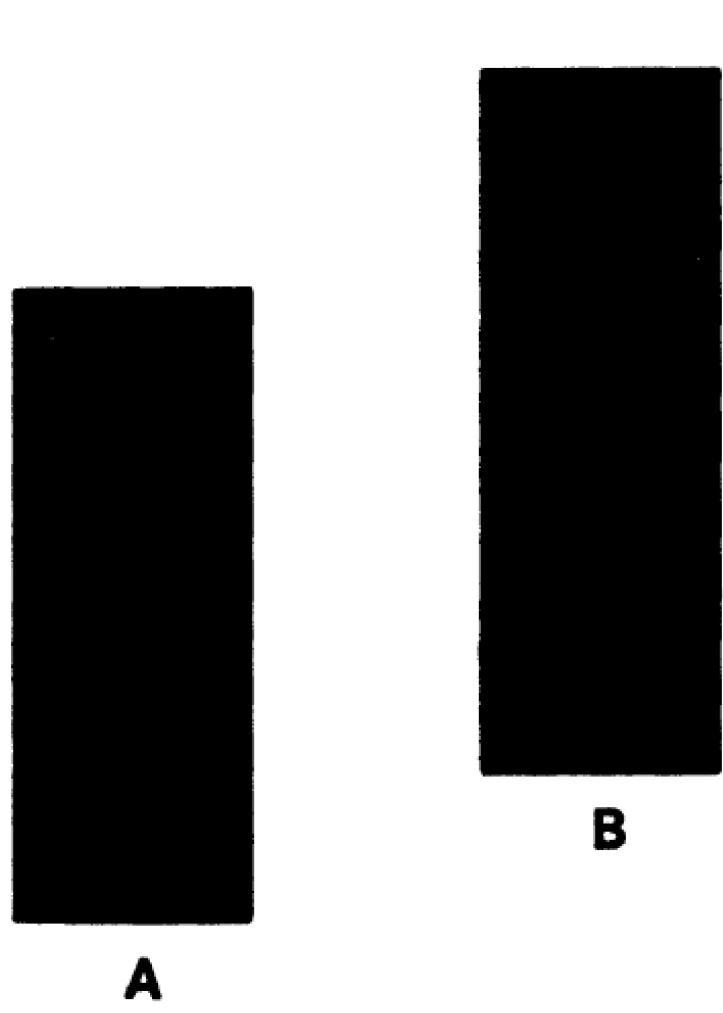
\includegraphics[width = 0.32\textwidth]{BarsClevelandUnFramed.jpg}}
  \only<2>{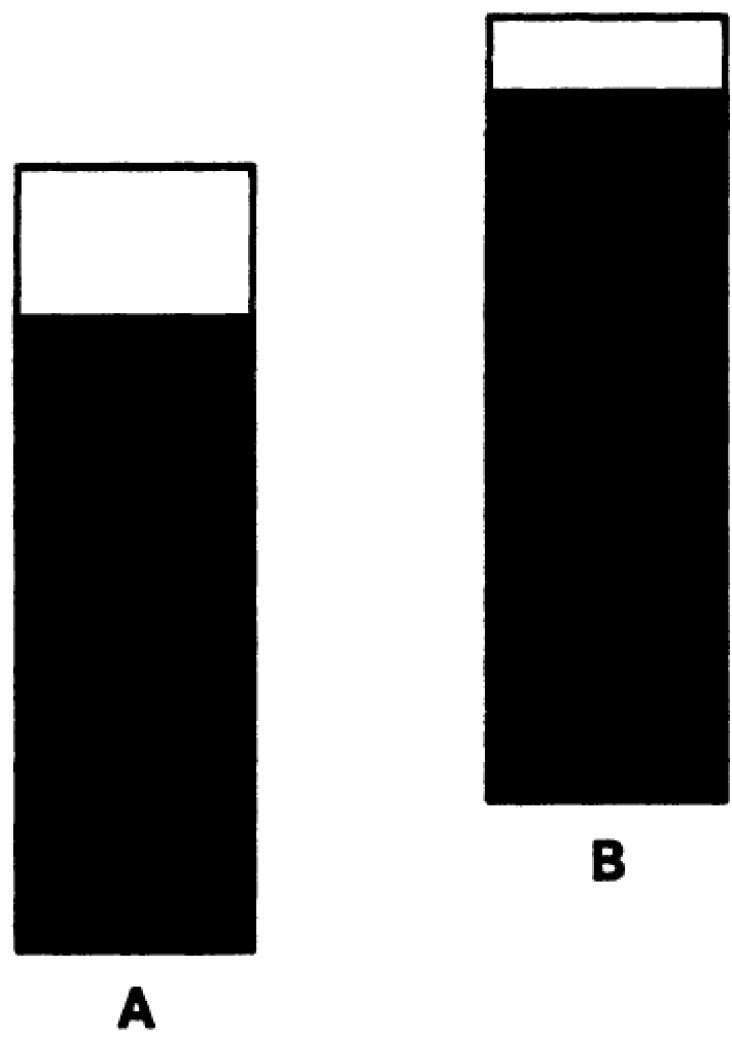
\includegraphics[width = 0.32\textwidth]{BarsClevelandFramed.jpg}}
  \only<1-2>{\textcolor{gris}{\footnotesize{Source: \cite{Cleveland1984}}} \hfill \textcolor{brique}{\textbf{Poll}} }
  \only<3>{ 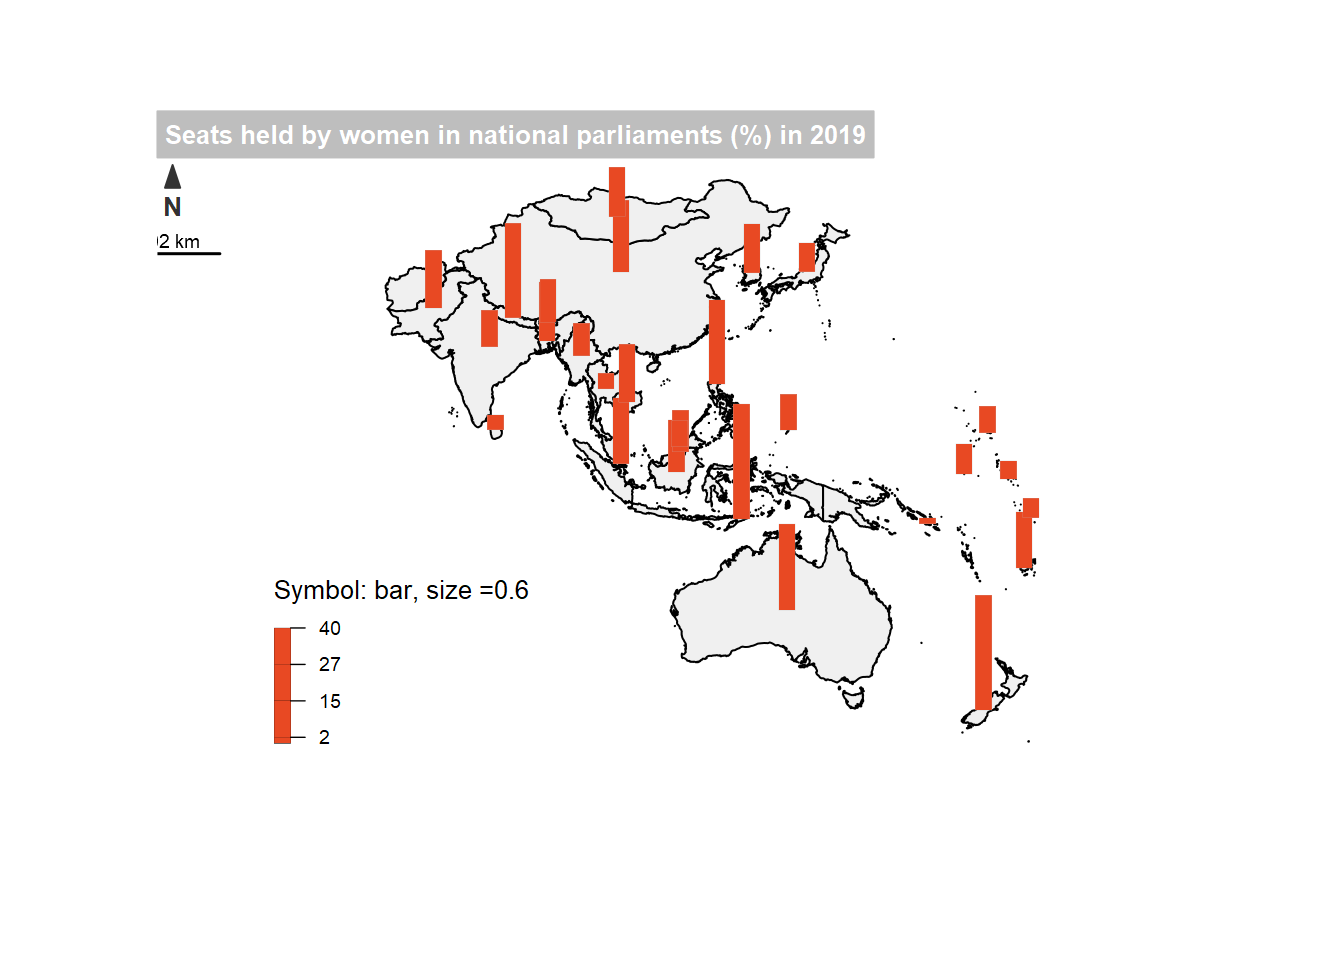
\includegraphics[width =0.9\textwidth]{BubbleMapBars.png} }
  \only<4>{ 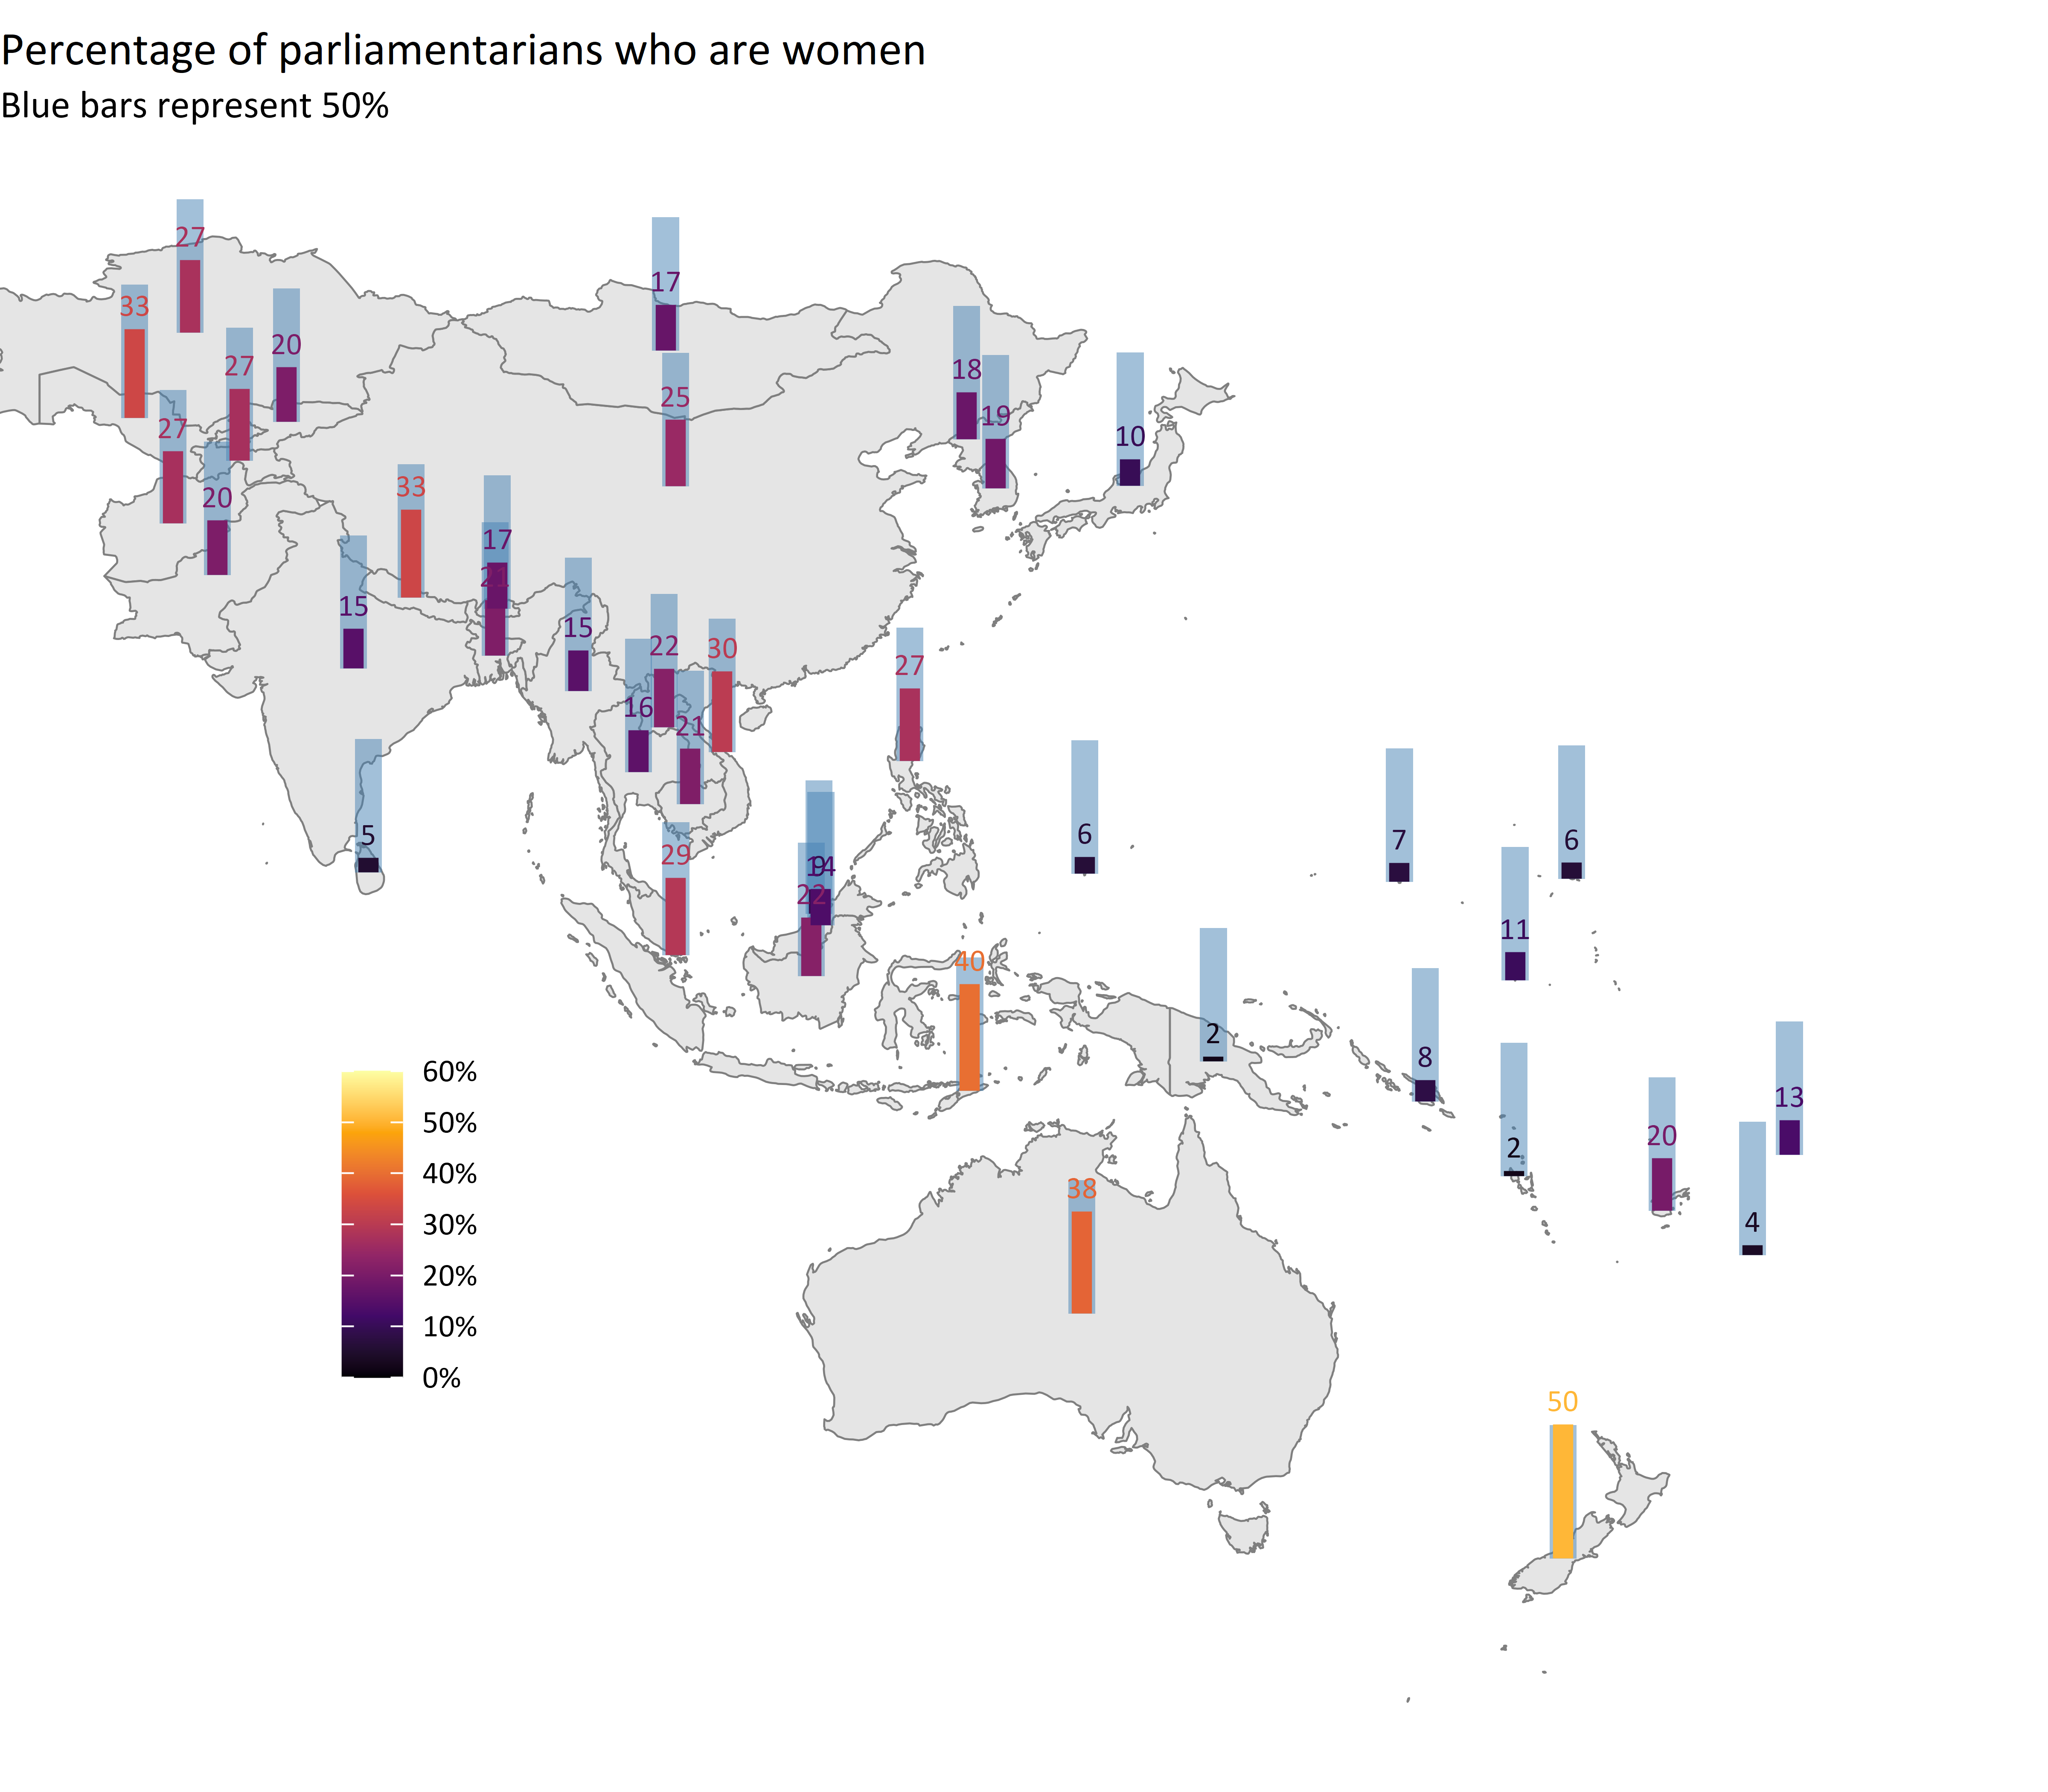
\includegraphics[width =0.65\textwidth]{PEllisGaugeMap.png} }
\end{itemize}
\end{center}
\end{frame}





%
%\begin{frame}
%\frametitle{\textcolor{brique}{[- \textbf{Rule \#8: Use [unaligned] bars} -]}}
%\begin{center}
%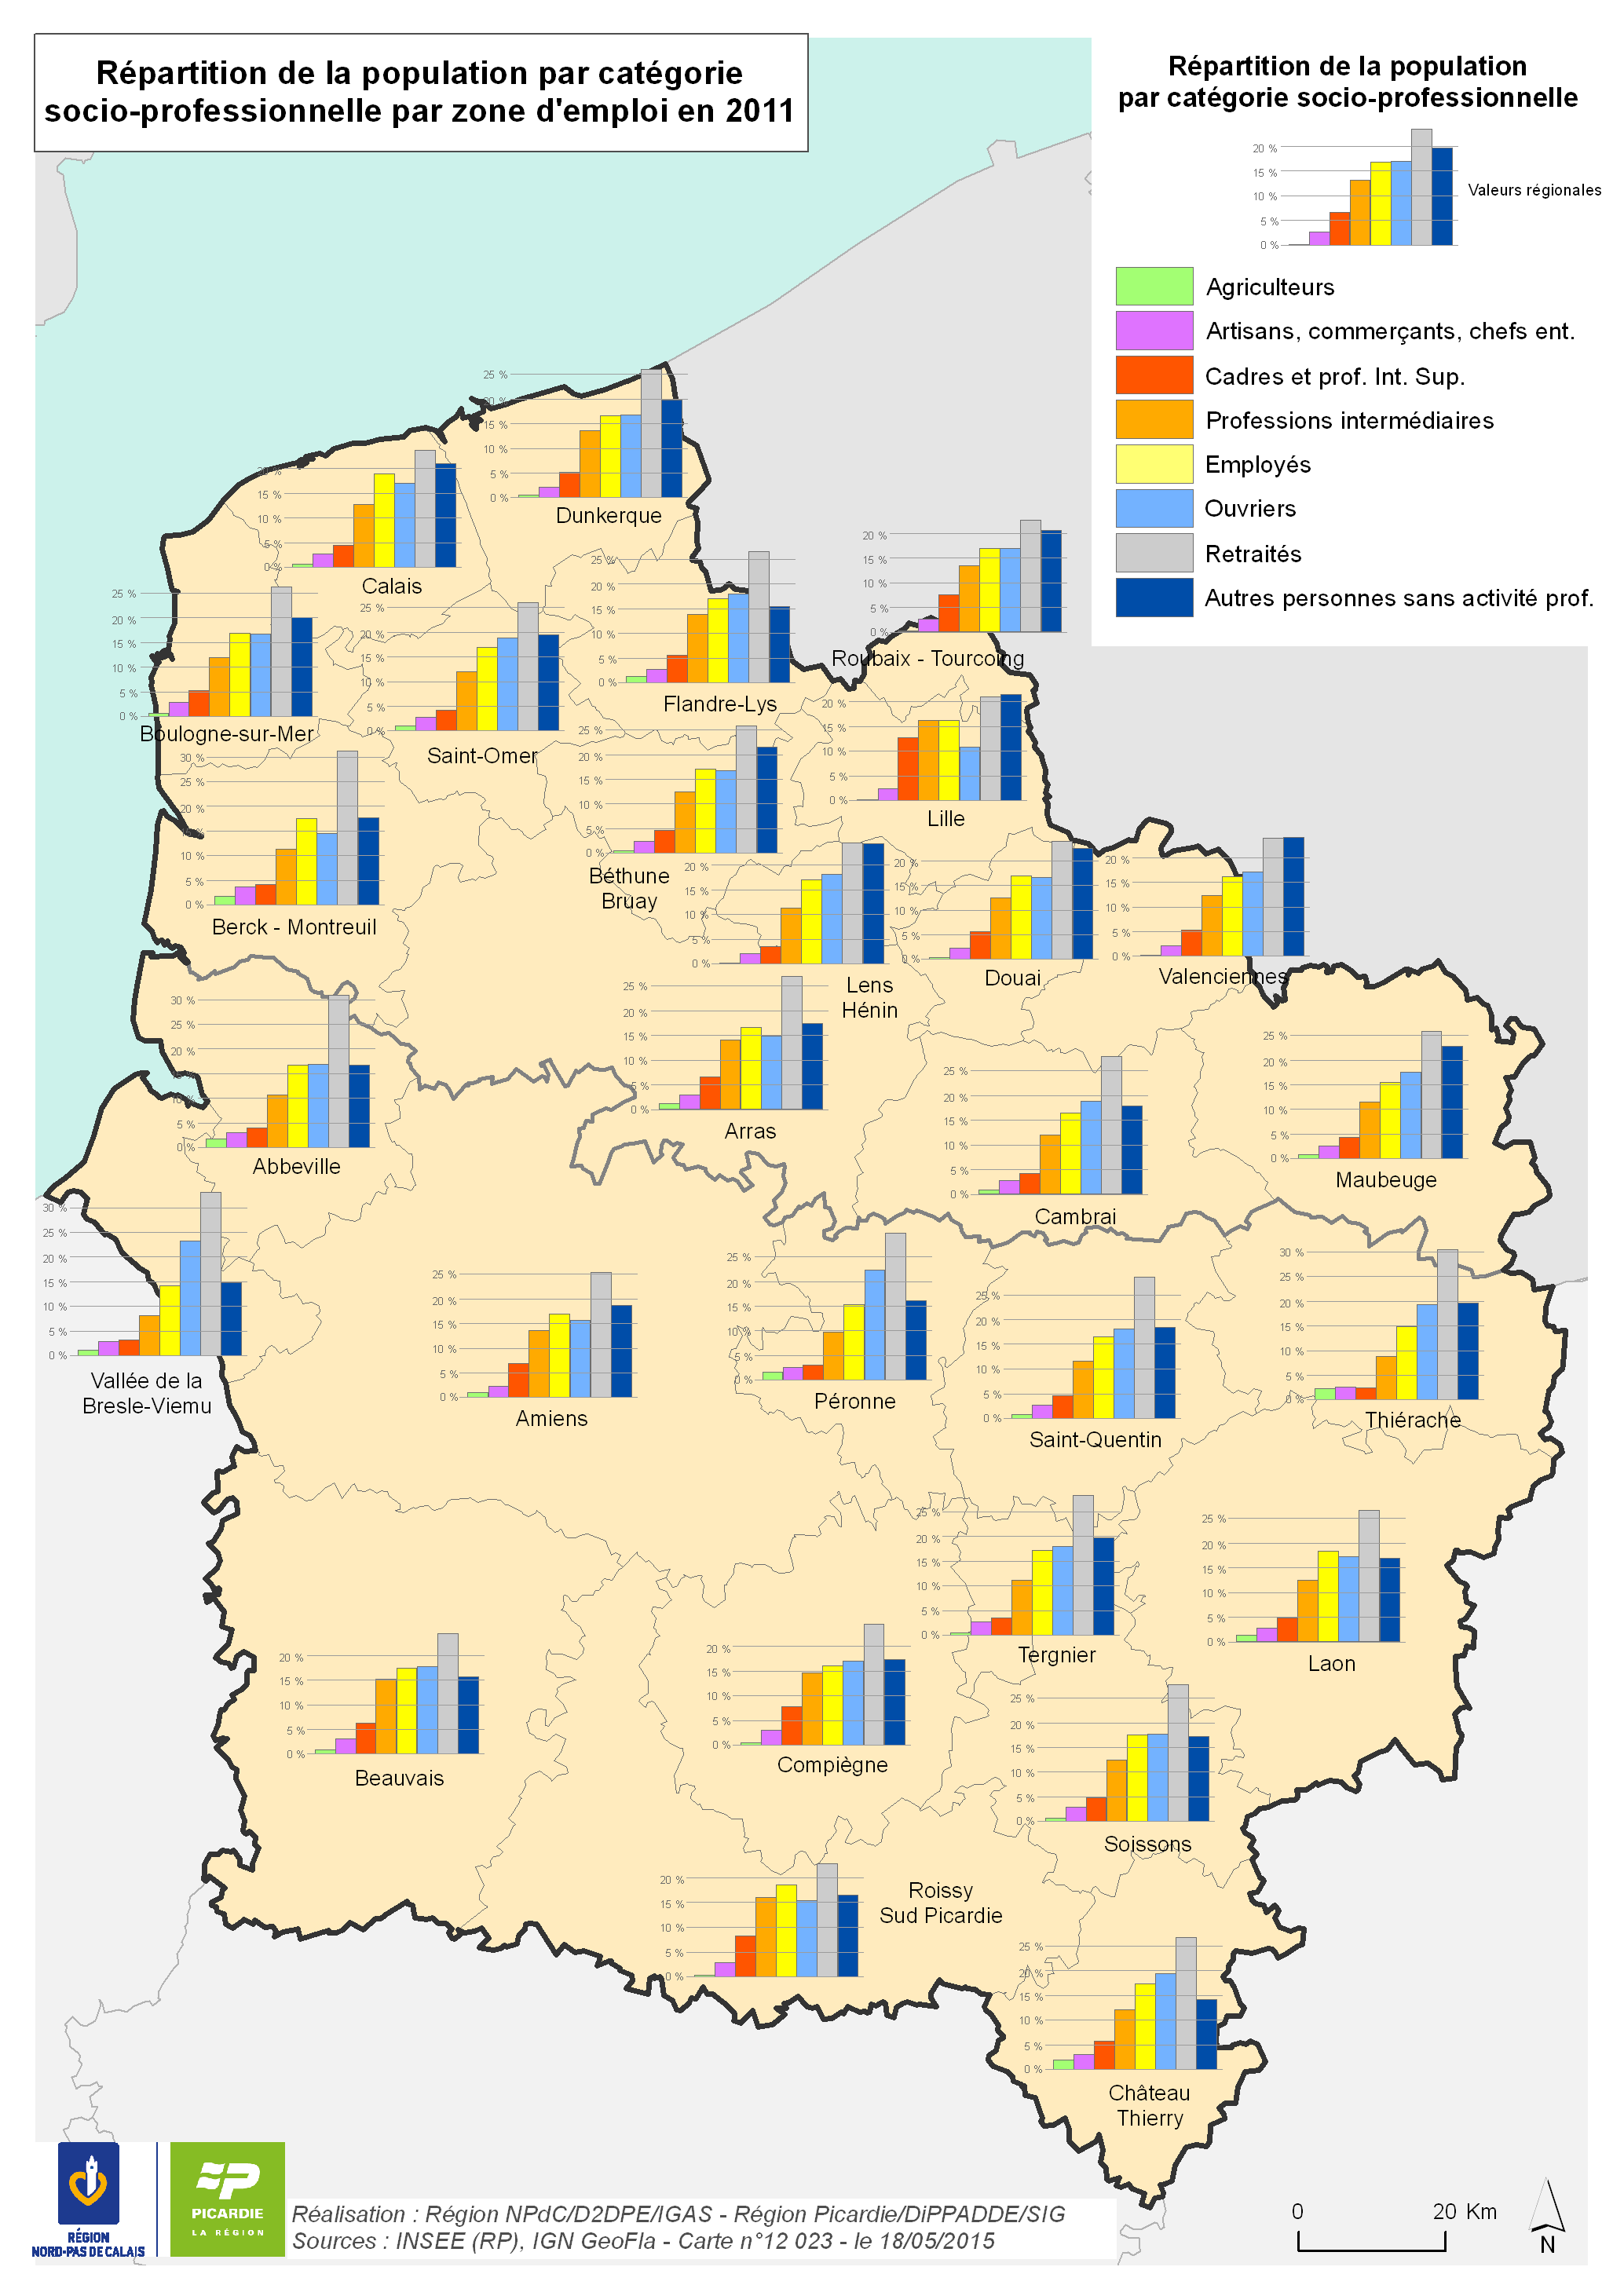
\includegraphics[width = 0.55\textheight]{CarteBarresRepartitionPopCsp2011.png}
%\end{center}
%\textcolor{gris}{\footnotesize{Source: \href{https://cartes.hautsdefrance.fr/?q=system/files/12023_repartition_population_pa_csp_2011.png }{Cartotheque (haut de France)}}}
%\end{frame}

%
%
%\begin{frame} % Cover slide
%\frametitle{\textcolor{brique}{[- \textbf{Rule \#8-bis: Use Stacked barcharts  } -]}}
%\begin{figure}
%\href{http://bl.ocks.org/marcdhansen/1ace92ea6344aa05bbac}{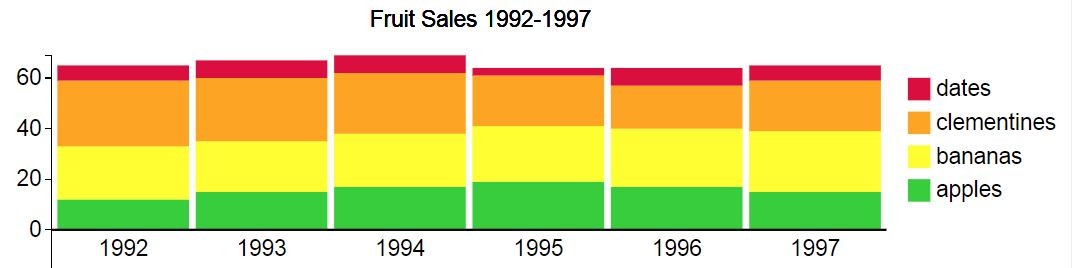
\includegraphics[width = 0.95\textwidth]{InteractiveHistograms-0.jpg}}
%%\caption{Diagramme en bâtons  : Les ventes de bananes (jaune) ont t'elles augmentées ? Celles des clementines ?}
%\end{figure}
%\textcolor{gris}{\footnotesize{Source: \cite{Dix1998}}}    \hfill \textcolor{brique}{\textbf{Poll}}
%\end{frame}
%
%\begin{frame} % Cover slide
%\frametitle{\textcolor{brique}{[- \textbf{Solution \#8-bis: Align the bars!} -]}}
%\begin{figure}
%\href{http://bl.ocks.org/marcdhansen/1ace92ea6344aa05bbac}{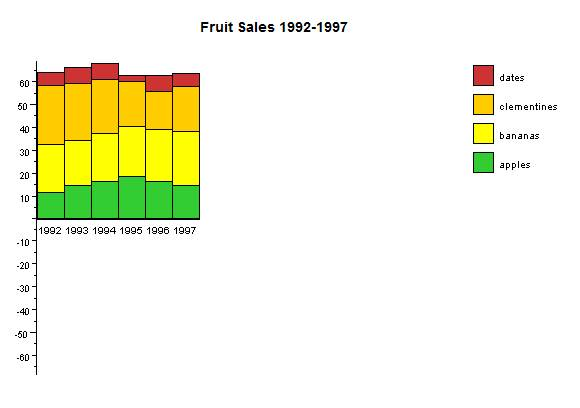
\includegraphics[width=0.4\textwidth]{FruitsSales1.jpg}}
%\href{http://bl.ocks.org/marcdhansen/1ace92ea6344aa05bbac}{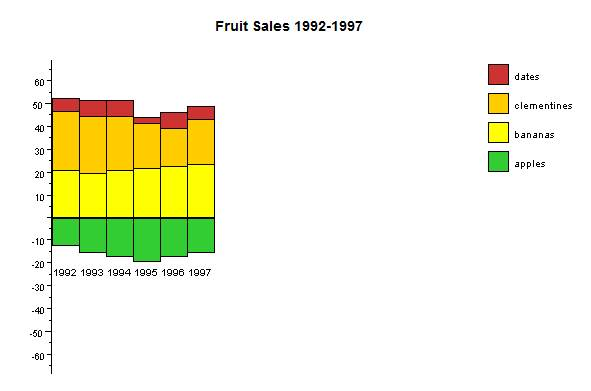
\includegraphics[width=0.4\textwidth]{FruitsSales2.jpg}} \\
%\href{http://bl.ocks.org/marcdhansen/1ace92ea6344aa05bbac}{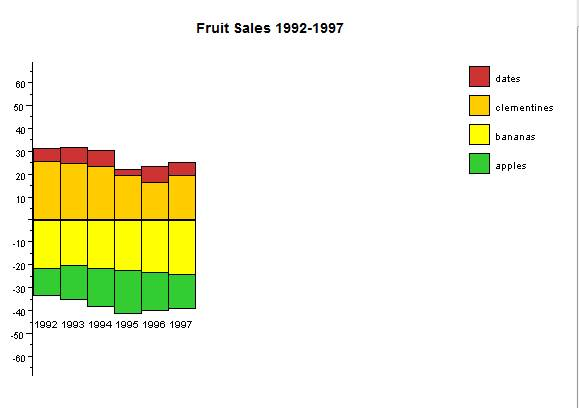
\includegraphics[width=0.4\textwidth]{FruitsSales3.jpg}}
%\href{http://bl.ocks.org/marcdhansen/1ace92ea6344aa05bbac}{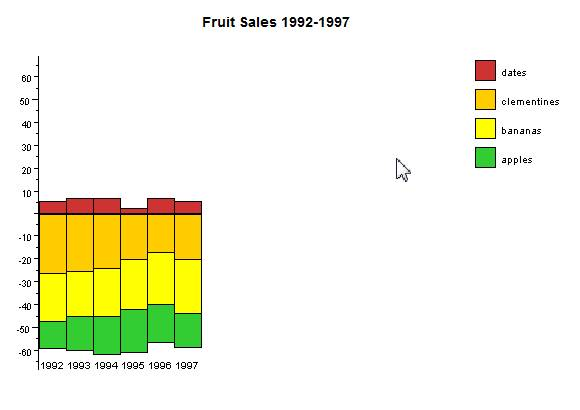
\includegraphics[width=0.4\textwidth]{FruitsSales4.jpg}}
%   \caption{From \cite{Dix1998} example}
%\end{figure}
%\vfill
%See also the \href{http://bl.ocks.org/marcdhansen/1ace92ea6344aa05bbac}{dynamic version}
%\end{frame}

%\begin{frame} % Cover slide
%\frametitle{\textcolor{brique}{[- \textbf{Rule \#8-bis: Use Stacked barcharts  } -]}}
%Kind of stupid example:
%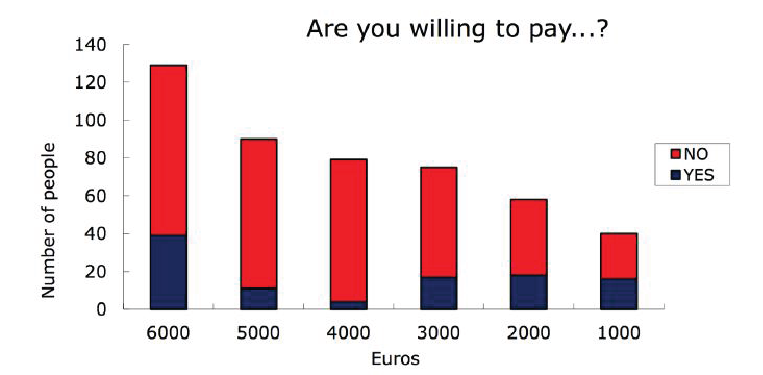
\includegraphics[width = 0.9\textwidth]{Yes-NO-TsEconomist12-2016.pdf}  \\
%
%\textcolor{gris}{\footnotesize{Source: \href{https://thetseconomist.files.wordpress.com/2017/06/12th-issue.pdf}{The TSEconomics Journal (TSE)}}}
%
%%TSE students were initially asked: would you be willing to pay 6000 euros for a masters in TSE? If they answered no, we repeated the question with a lower amount by an interval of 1000 euros (Notice that the plot is about the marginal number who are willing or not to pay the fee, and not the cumulative one) Source: survey
%
%\end{frame}


\section{Rule 9}

\begin{frame} % Cover slide
\frametitle{\textcolor{brique}{[- \textbf{Rule \#9: Use lines} (lots of them!)   -]}}
Observe this graphic carefully:
\begin{figure}[h]
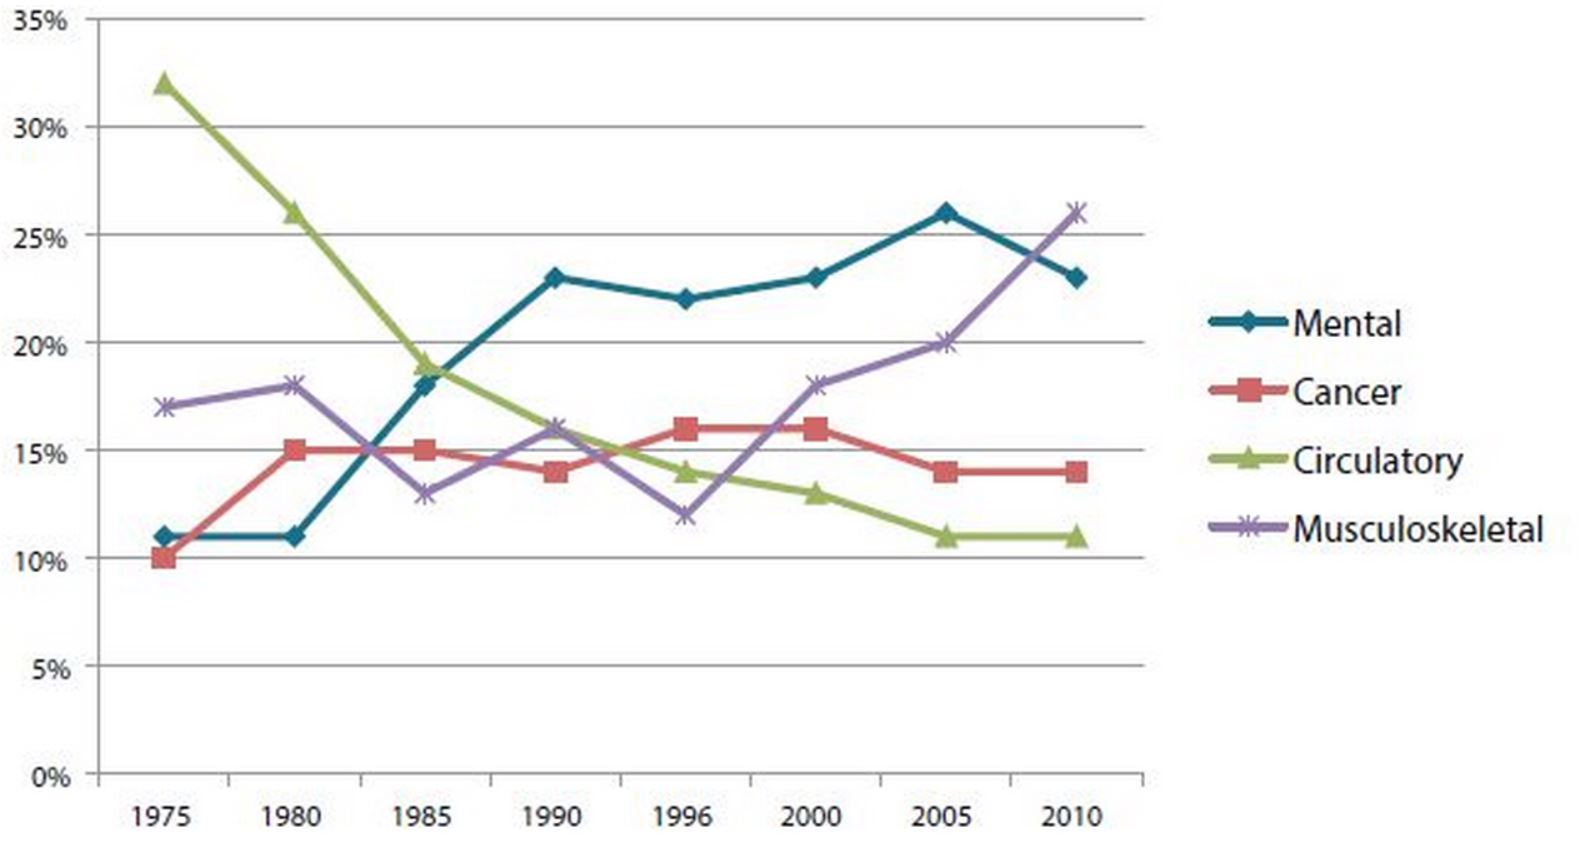
\includegraphics[width = 0.9\textwidth]{Spaghetti0.jpg}
\caption{Major Cause of Worker Disability (1975-2010) (J. Schwabish, 2014).  \hfill \textcolor{brique}{\textbf{Poll}}  }
\end{figure}
\end{frame}

\begin{frame} % Cover slide
\frametitle{\textcolor{brique}{ Can we answer  \textbf{legitimate}  questions? }}
\begin{center}
{\huge \textcolor{brique}{\textbf{Poll}} }
\end{center}
\end{frame}


\begin{frame} % Cover slide
\frametitle{\textcolor{brique}{[- \textbf{Solution \#9: Use \textit{small multiples}}   -]}}
\begin{figure}[h]
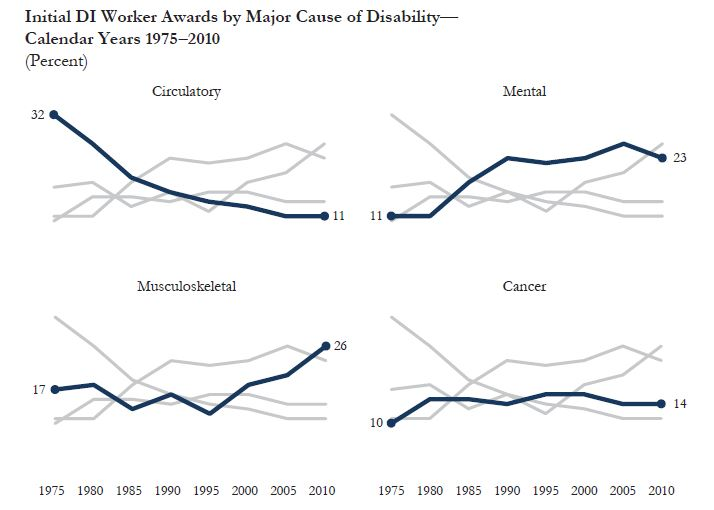
\includegraphics[width =0.75\textwidth]{Spaghetti2.jpg}
\caption{Major Cause of Disability - 1975-2010 (J. Schwabish, 2014).  }
\end{figure}
\end{frame}

%\begin{frame}
%\frametitle{\textcolor{brique}{[- \textbf{Rule \#9bis: Use lines} (Compare)   -]}}
%For each graph, compute the difference between the 2 lines. \hfill \textcolor{brique}{\textbf{Poll}}
%\begin{enumerate}
%   \item<+->[]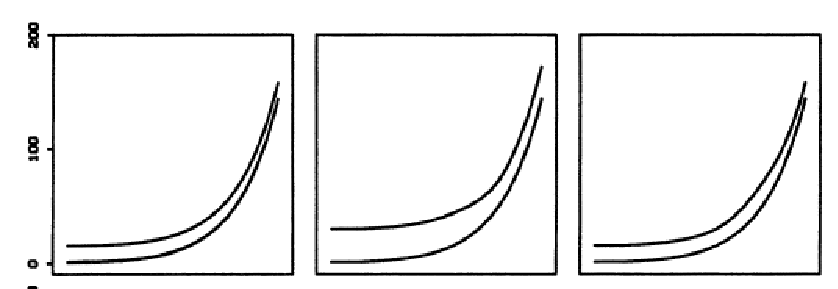
\includegraphics[width = 0.65\textwidth]{Curves1.pdf}
%   \item<+->[]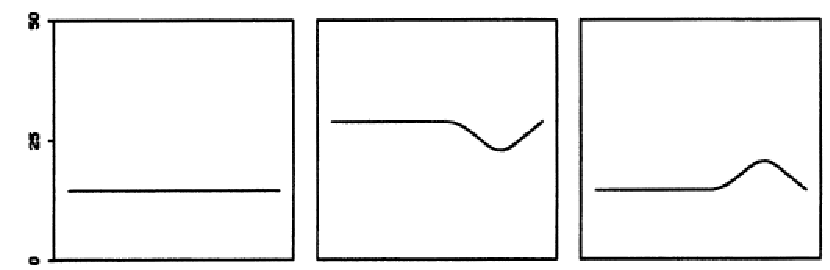
\includegraphics[width = 0.65\textwidth]{curves1-diff.pdf}
%   \item<+->[] From \cite{Cleveland1984}
%\end{enumerate}
%\end{frame}

%\begin{frame}
%\frametitle{\textcolor{brique}{[- \textbf{Rule \#6bis: Compare lines} -]}}
%\begin{enumerate}
%   \item[]
%\only<1>{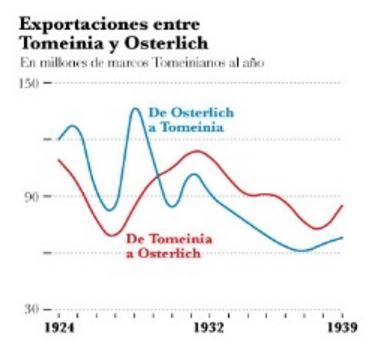
\includegraphics[width = 0.6\textwidth]{Lines-Cairo.jpg}}
%\only<2>{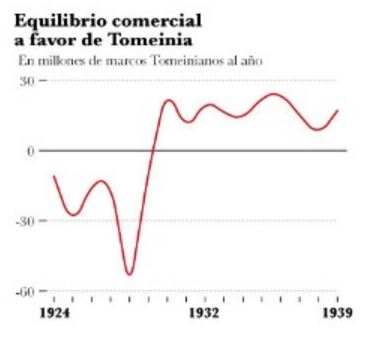
\includegraphics[width = 0.6\textwidth]{Lines-Cairo-diff.jpg}}
%\only<2>{\textcolor{gris}{\footnotesize{From \cite{Cairo2012}}}}
%\end{enumerate}
%\end{frame}
%
%\begin{frame}
%\frametitle{\textcolor{brique}{[- \textbf{Rule \#6bis: Compare lines}  -]}}
%\begin{enumerate}
%   \item<+->[]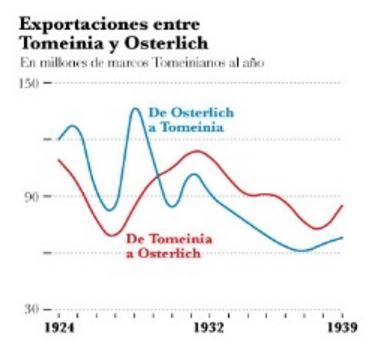
\includegraphics[width = 0.3\textwidth]{Lines-Cairo.jpg}
%   \item<+->[]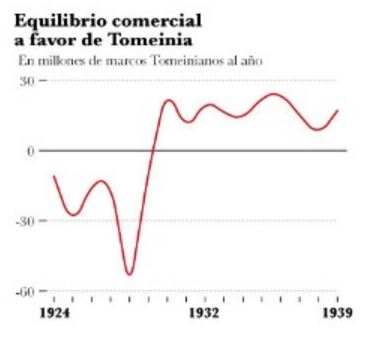
\includegraphics[width = 0.3\textwidth]{Lines-Cairo-diff.jpg}
%   \item<+->[] \textcolor{gris}{\footnotesize{From \cite{Cairo2012}}}
%\end{enumerate}
%\end{frame}
%

%
%\begin{frame} % Cover slide
%\frametitle{Very usual ``\textit{Mistake}'' II... }
% \begin{itemize}
% \item<+->[] 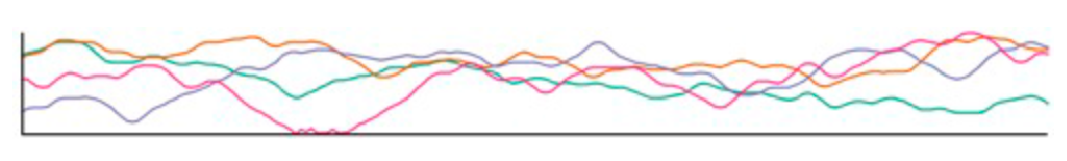
\includegraphics[width = 1.0\textwidth]{MunznerLinesClassic.pdf}
% \item <+-> What do you see here ?
% \item<+->[] 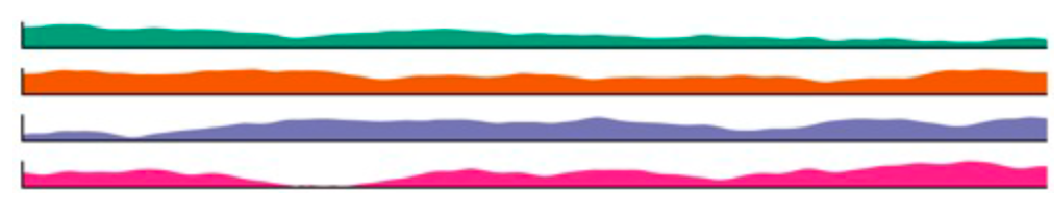
\includegraphics[width = 1.0\textwidth]{MunznerLinesMultiples.pdf}
% \item<+->[] Easier to see the trend of each curve...
%  \item<+->[] Idea shared by \cite{Gelman2004}  and \cite{Munzner2014}  %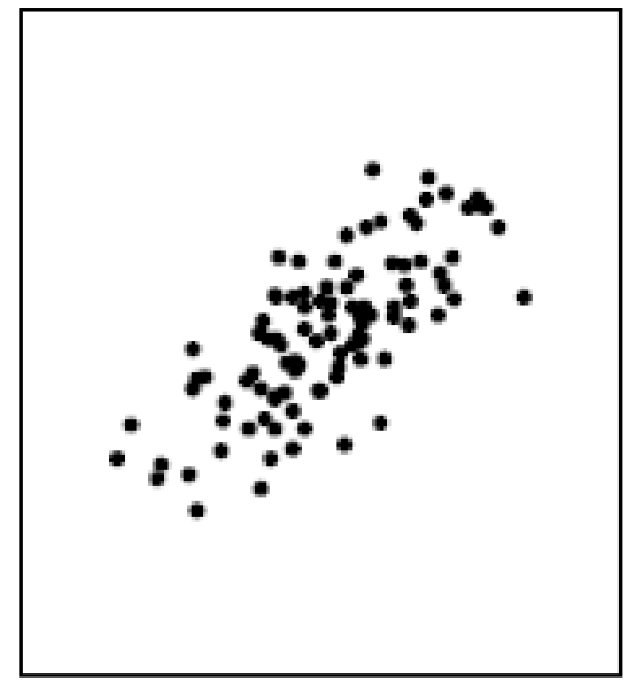
\includegraphics[width = 0.5\textwidth]{Buja-Exemple2.pdf}
% \end{itemize}
%\end{frame}
%

\section{Rule 10}

\begin{frame} % Cover slide
\frametitle{\textcolor{brique}{[- \textbf{Rule \#10: Use radar plots} (or Web plots)  -]}}
\begin{center}
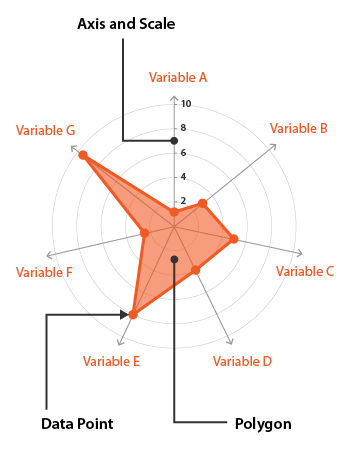
\includegraphics[width = 0.4\textwidth]{radar_chart.png}
\end{center}
\textcolor{gris}{\footnotesize{Source: \href{https://datavizcatalogue.com/methods/radar_chart.html}{Dataviz catalogue}}}
\end{frame}


\begin{frame} % Cover slide
\frametitle{\textcolor{brique}{[- \textbf{Rule \#10: Use radar plots}  -]}}
\begin{figure}[h]
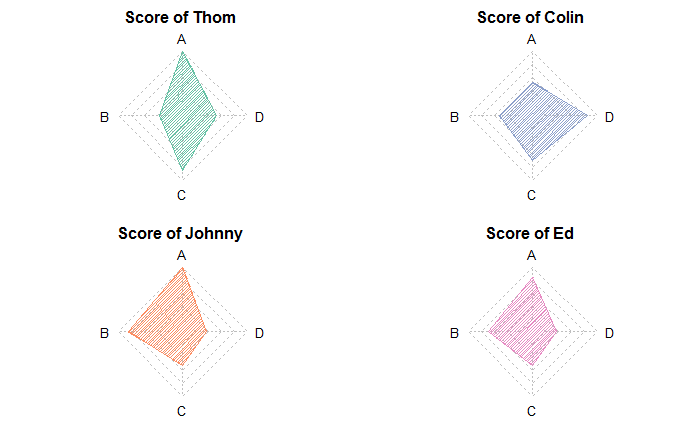
\includegraphics[width = 0.7\textwidth]{Radar1.png}
\end{figure}
\textcolor{gris}{\footnotesize{Source: \href{http://data.visualisation.free.fr/Blog/Why-you-should-never-use-radar-plots.nb.html}{Xtophe's blog: Why you should never use radar plots}}} \hfill \textcolor{brique}{\textbf{Poll}}
\end{frame}

\begin{frame} % Cover slide
\frametitle{\textcolor{brique}{[- \textbf{Rule \#10: Use radar plots}  -]}}
\begin{figure}[h]
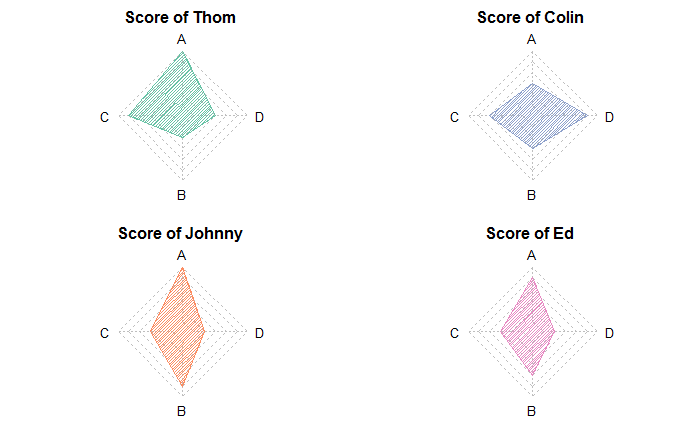
\includegraphics[width = 0.7\textwidth]{Radar2.png}
\end{figure}
\textcolor{gris}{\footnotesize{Source: \href{http://data.visualisation.free.fr/Blog/Why-you-should-never-use-radar-plots.nb.html}{Xtophe's blog: Why you should never use radar plots}}}
\end{frame}


\begin{frame}
\frametitle{\textcolor{brique}{[- \textbf{Rule \#10: Use radar plots}  -]}}
\begin{center}
\begin{enumerate}
   \only<1>{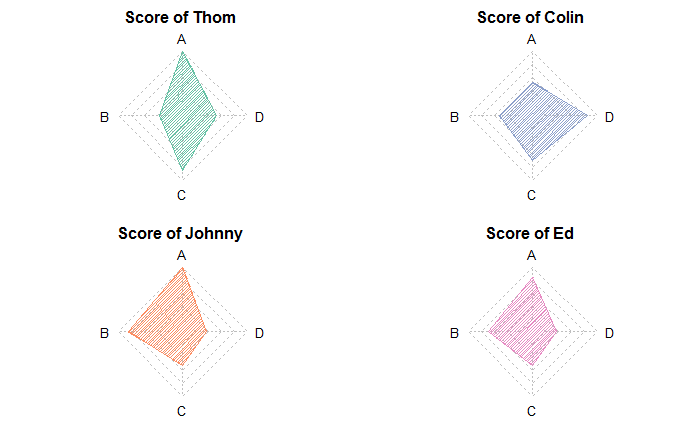
\includegraphics[width = 0.5\textwidth]{Radar1.png}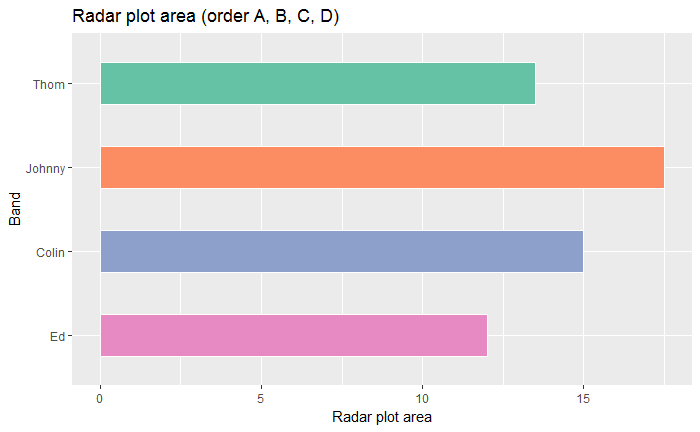
\includegraphics[width = 0.5\textwidth]{Radar-Bars1.png}}
   \only<2>{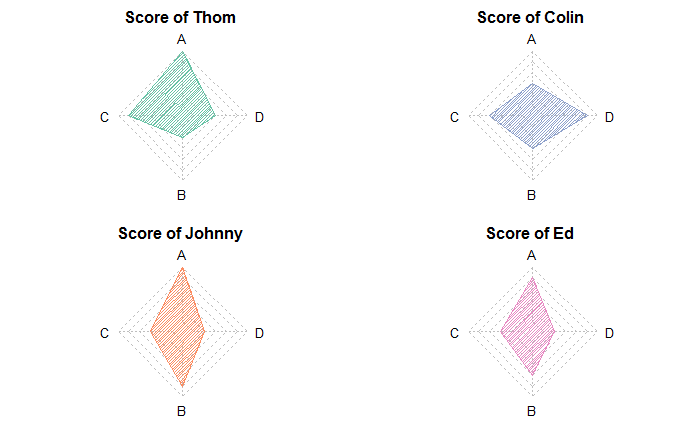
\includegraphics[width = 0.5\textwidth]{Radar2.png}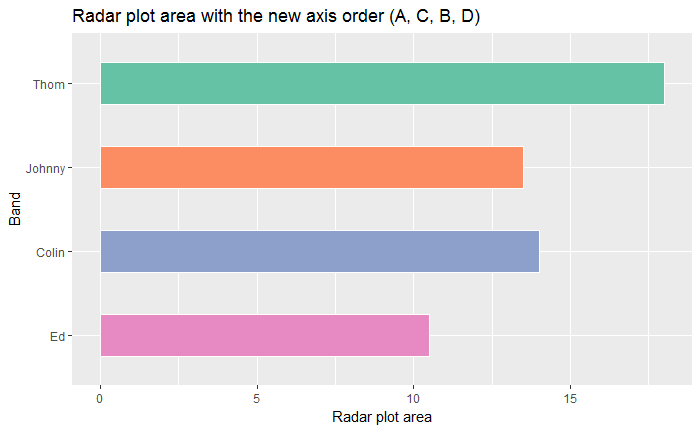
\includegraphics[width = 0.5\textwidth]{Radar-Bars2.png}}\\
\end{enumerate}
\end{center}
\textcolor{gris}{\footnotesize{Source: \href{http://data.visualisation.free.fr/Blog/Why-you-should-never-use-radar-plots.nb.html}{Xtophe's blog: Why you should never use radar plots}}}
\end{frame}



\section{Bonus}



\begin{frame}
\frametitle{\textcolor{brique}{[- \textbf{Super Rule:} Use Maps -]}}
2016 US Election "map" per \textit{counties} = \textbf{Land}
\begin{center}
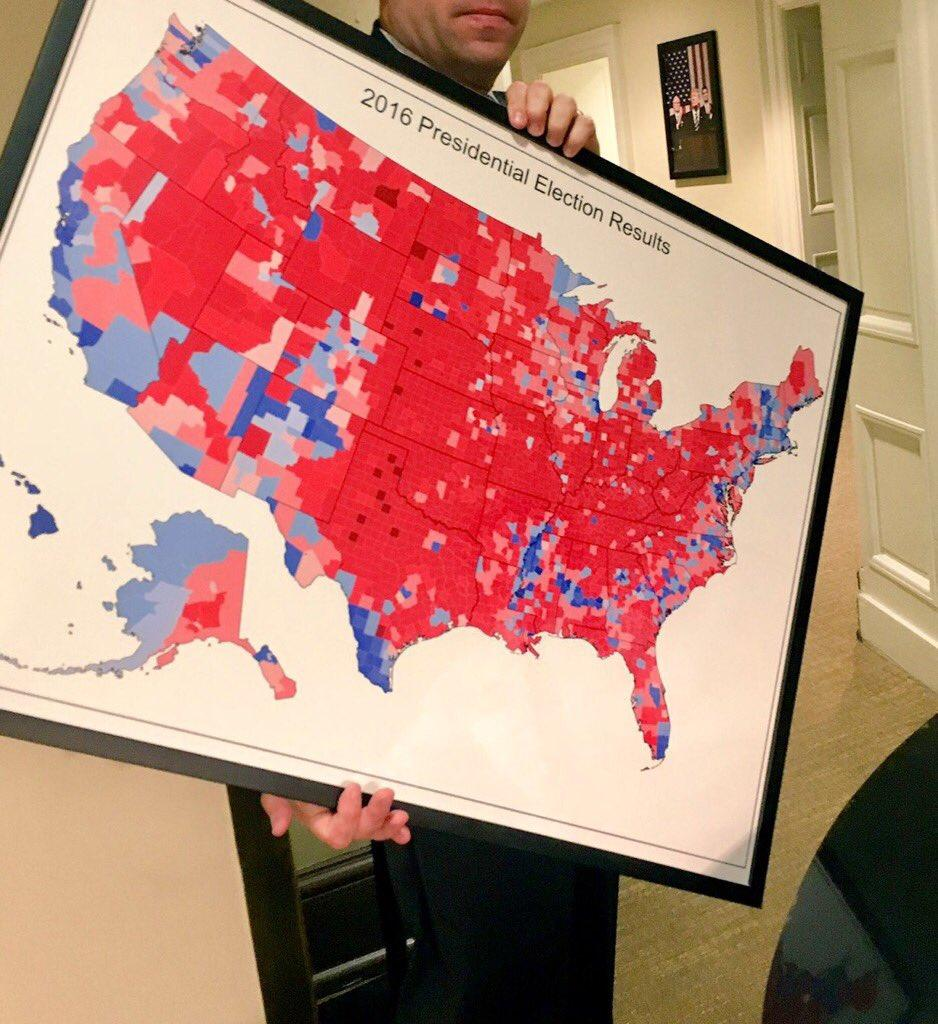
\includegraphics[width = 0.5\textwidth]{USA-Election-Trump-Framed-Map.jpg}
\end{center}
\textcolor{gris}{\footnotesize{Source: \href{https://twitter.com/TreyYingst/status/862669407868391424?s=20}{Trey Yingst (Fox News)}}}
\end{frame}


\begin{frame}
\frametitle{\textcolor{brique}{[- \textbf{Super Rule:} Use Maps -]}}
2016 US Election "map" (per \textit{counties})
\begin{center}
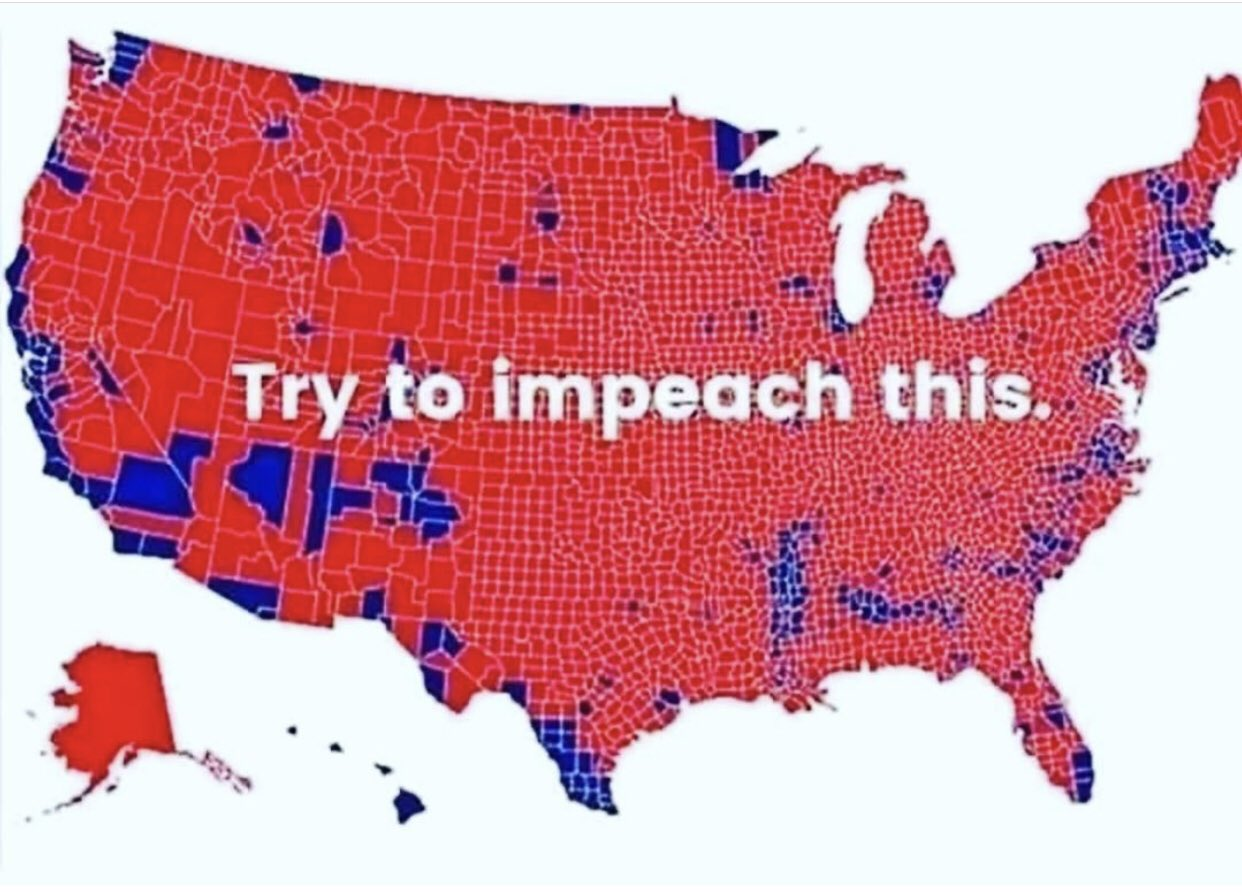
\includegraphics[width = 0.5\textwidth]{USA-Election-Trump-Impeach.jpg}
\end{center}
\textcolor{gris}{\footnotesize{Source: \href{https://twitter.com/LaraLeaTrump/status/1178030815671980032}{Lara Trump on Twitter (01/10/2019)} }}
\end{frame}

\begin{frame}
\frametitle{\textcolor{brique}{[- \textbf{Super Rule:} Use Maps -]}}
2016 US Election "map" (per \textit{nb of votes})
\begin{center}
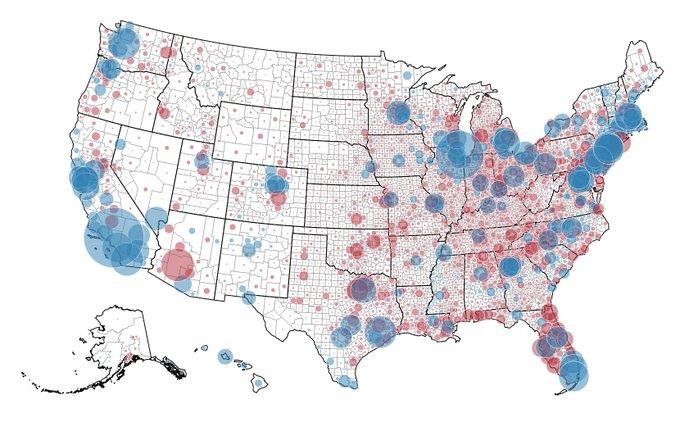
\includegraphics[width = 0.7\textwidth]{USA-Election-Trump-Circles.jpg}
\end{center}
\textcolor{gris}{\footnotesize{Source: \href{https://twitter.com/MInes_CR/status/1178347101513633792}{@MInesCR (Twitter) }}}
\end{frame}

\begin{frame}
\frametitle{\textcolor{brique}{[- \textbf{Super Rule:} Use Maps -]}}
2016 US Election "map" (per \textit{Nb of representatives})
\begin{center}
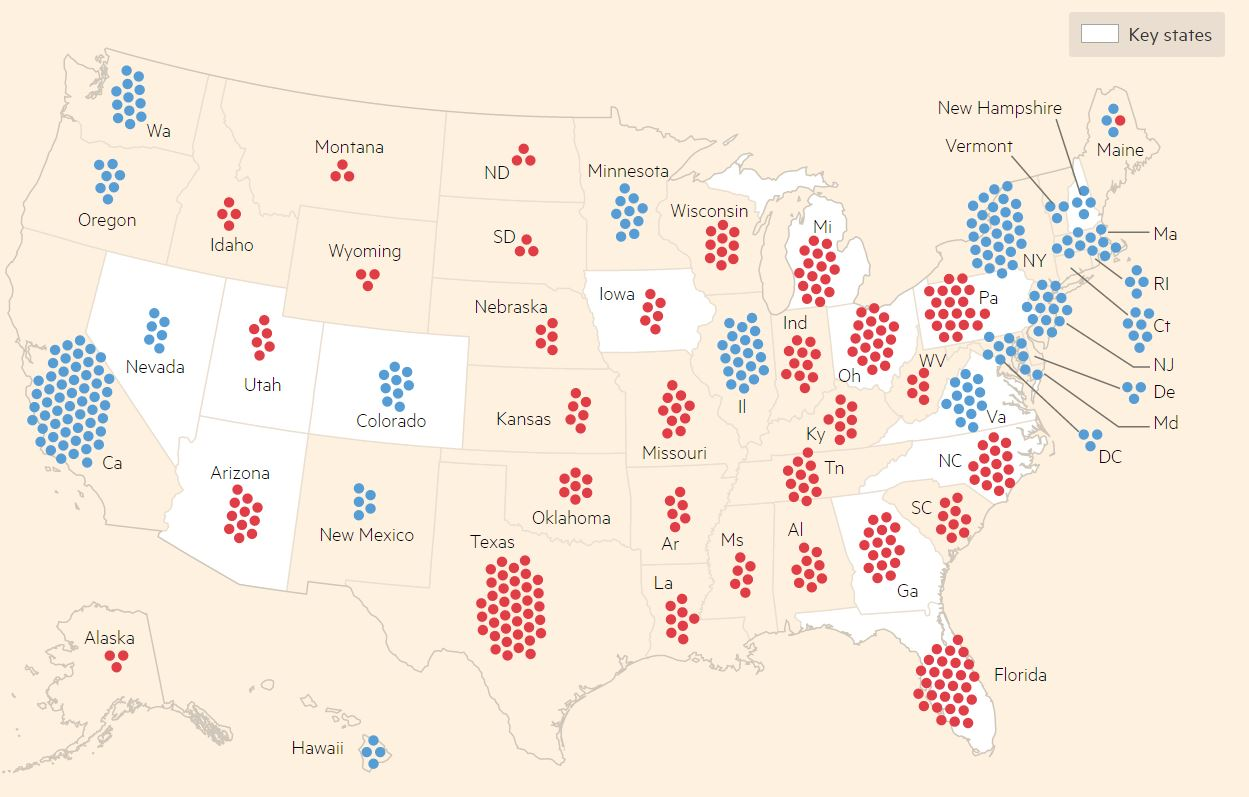
\includegraphics[width=0.7\textwidth]{US_election_dot_map2016.png}
\end{center}
\textcolor{gris}{\footnotesize{Source:  \href{https://ig.ft.com/us-elections/results}{\textit{Financial Times}}}}
\end{frame}


\begin{frame}
\frametitle{\textcolor{brique}{[- \textbf{Super Rule:} Use Maps -]}}
2016 US Election "map" (nb of \textit{votes})
\begin{center}
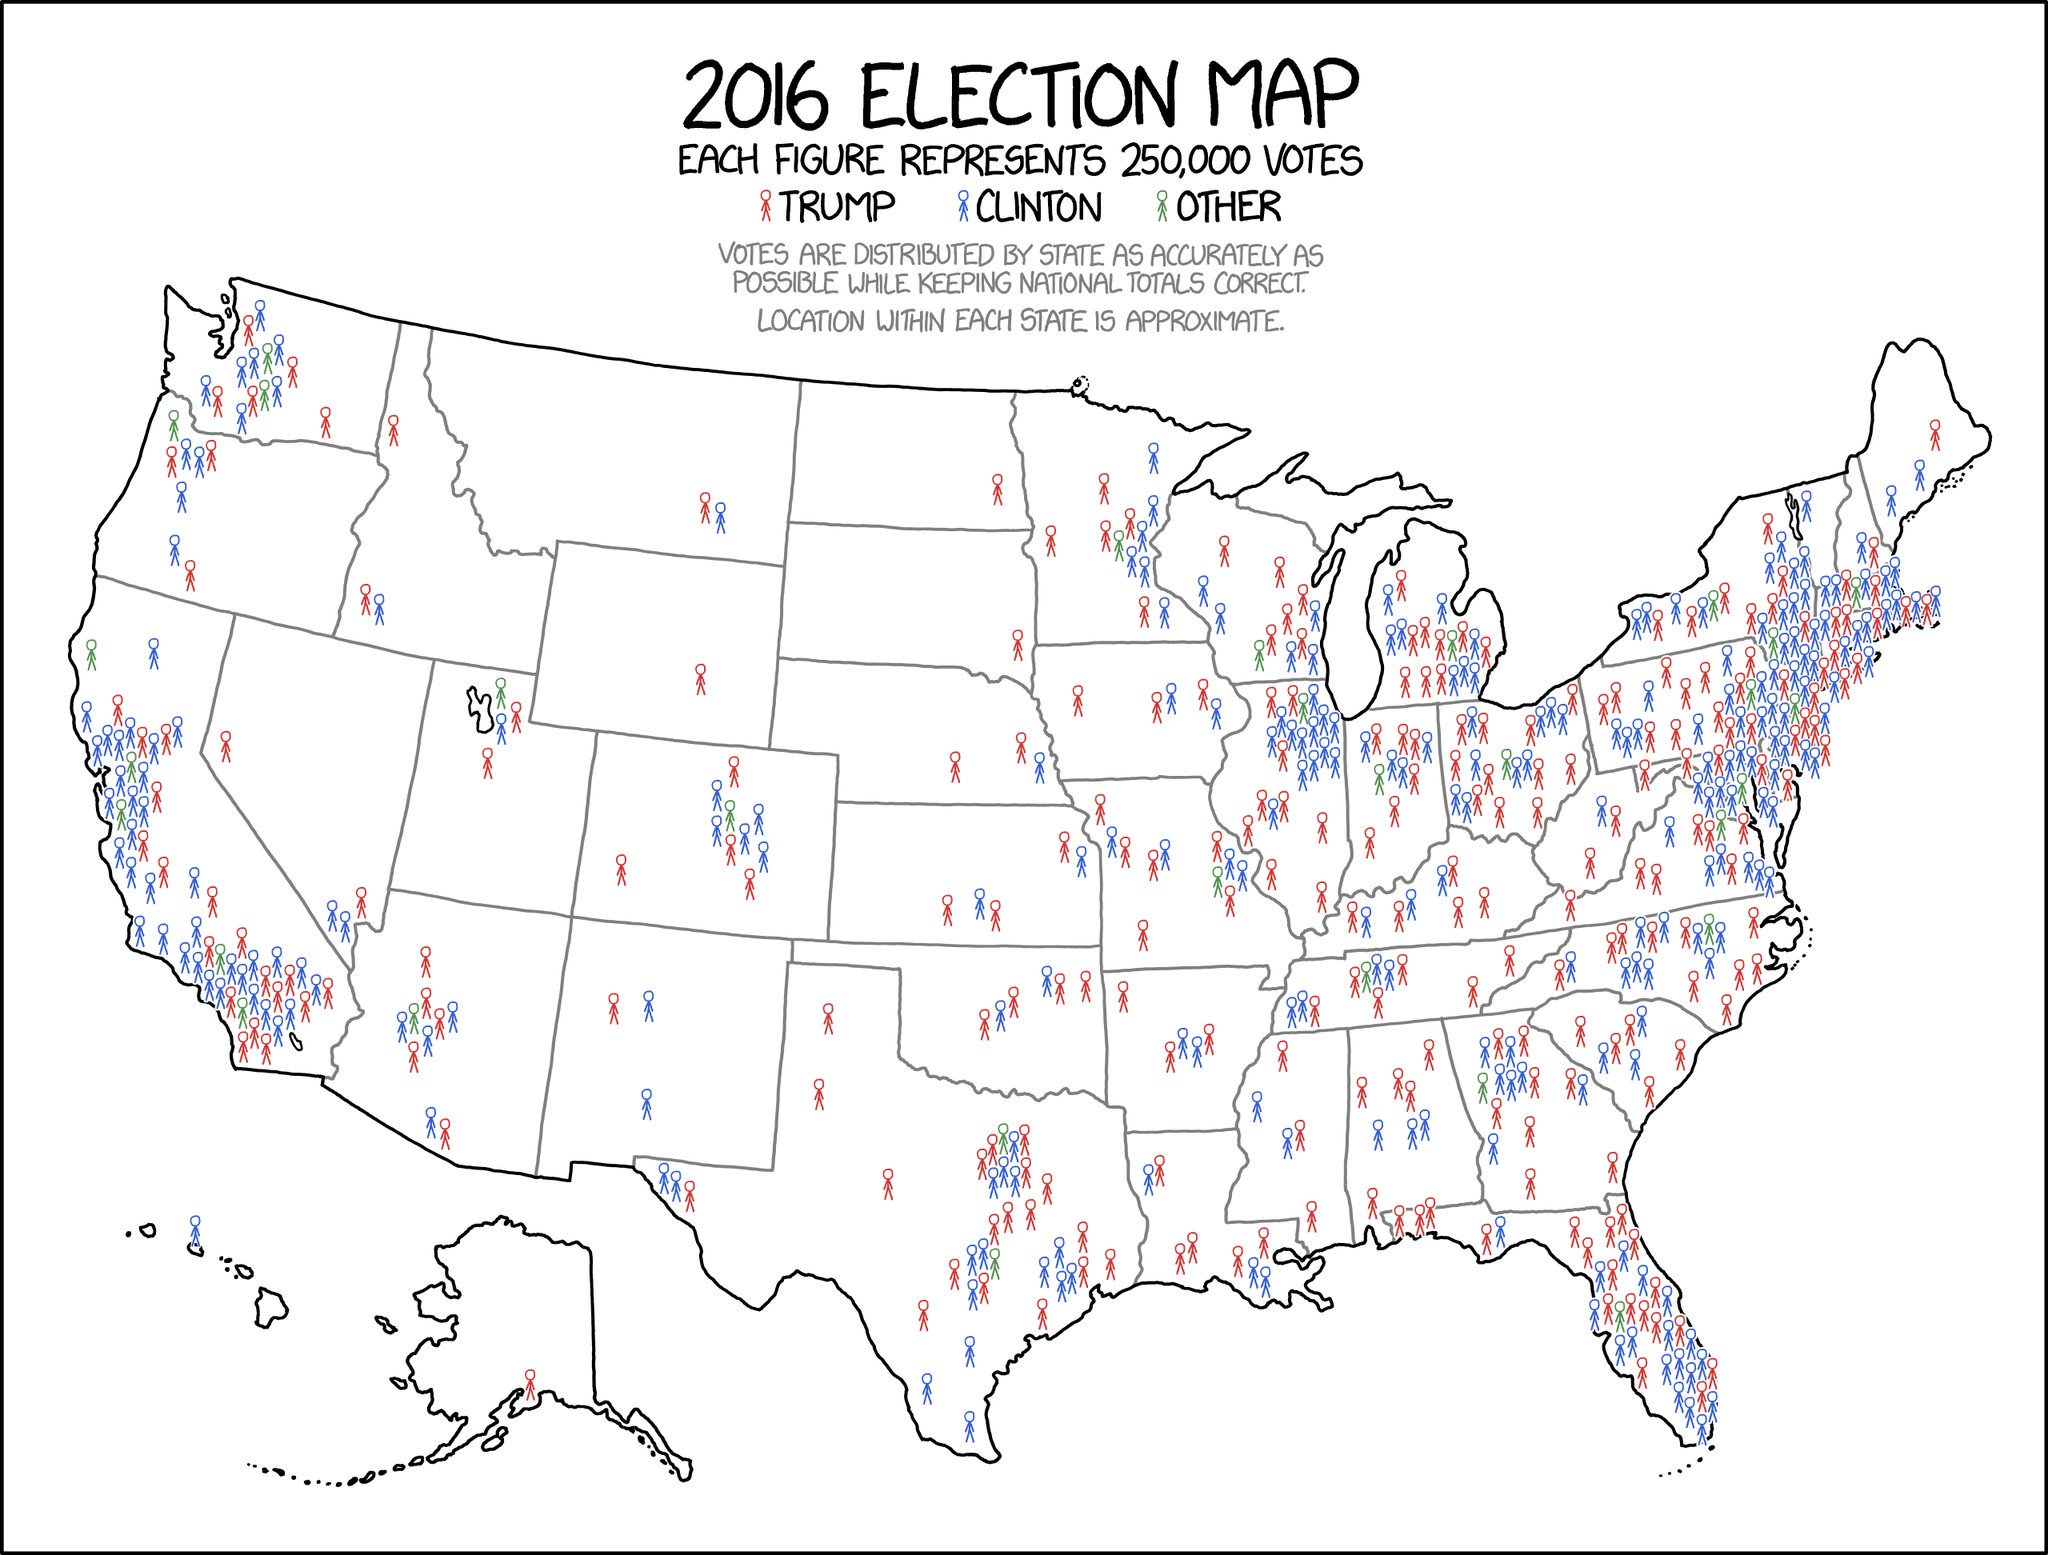
\includegraphics[width = 0.6\textwidth]{USA-Election-Trump-XKCD.jpg}
\end{center}
\textcolor{gris}{\footnotesize{Source: \href{https://xkcd.com/1939/}{XKCD }}}
\end{frame}



\begin{frame}
\frametitle{\textcolor{brique}{[- \textbf{Super Rule:} Use Maps -]}}

\begin{center}
\textbf{Land} doesn't vote, \textbf{people} do! \\

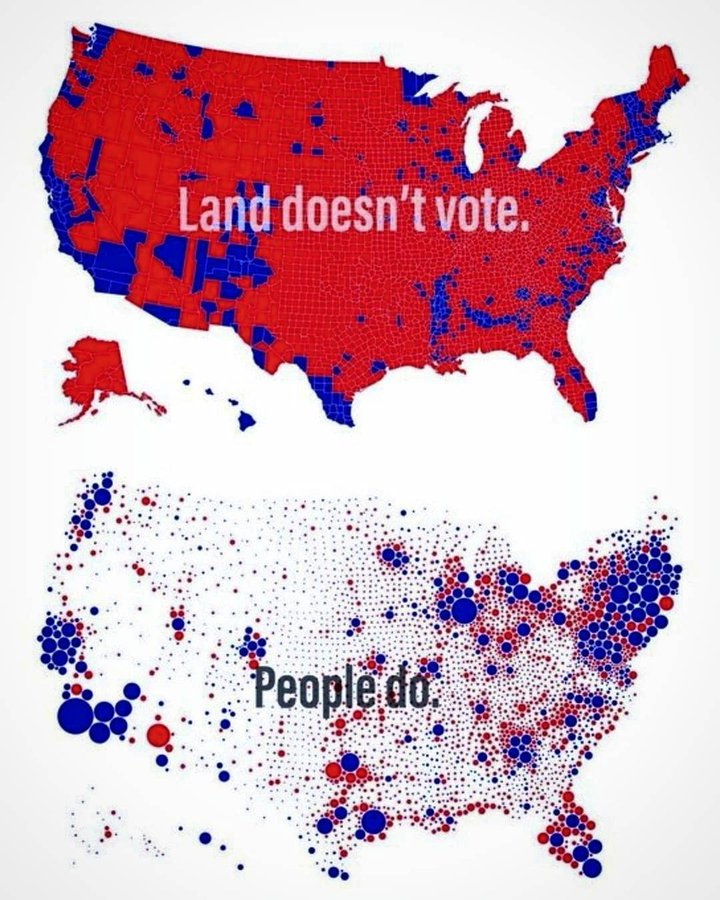
\includegraphics[width = 0.35\textwidth]{USA-Election-Trump-Land.jpg}
\end{center}
\textcolor{gris}{\footnotesize{Source: \href{https://twitter.com/zacharycoffin/status/1324674933679656964}{Zachary Coffin}}}
\end{frame}


\begin{frame} % Cover slide
\frametitle{\textcolor{brique}{[- \textbf{Bonus: Use [maps} -]}}
\begin{center}
\begin{itemize}
    \only<1>{ 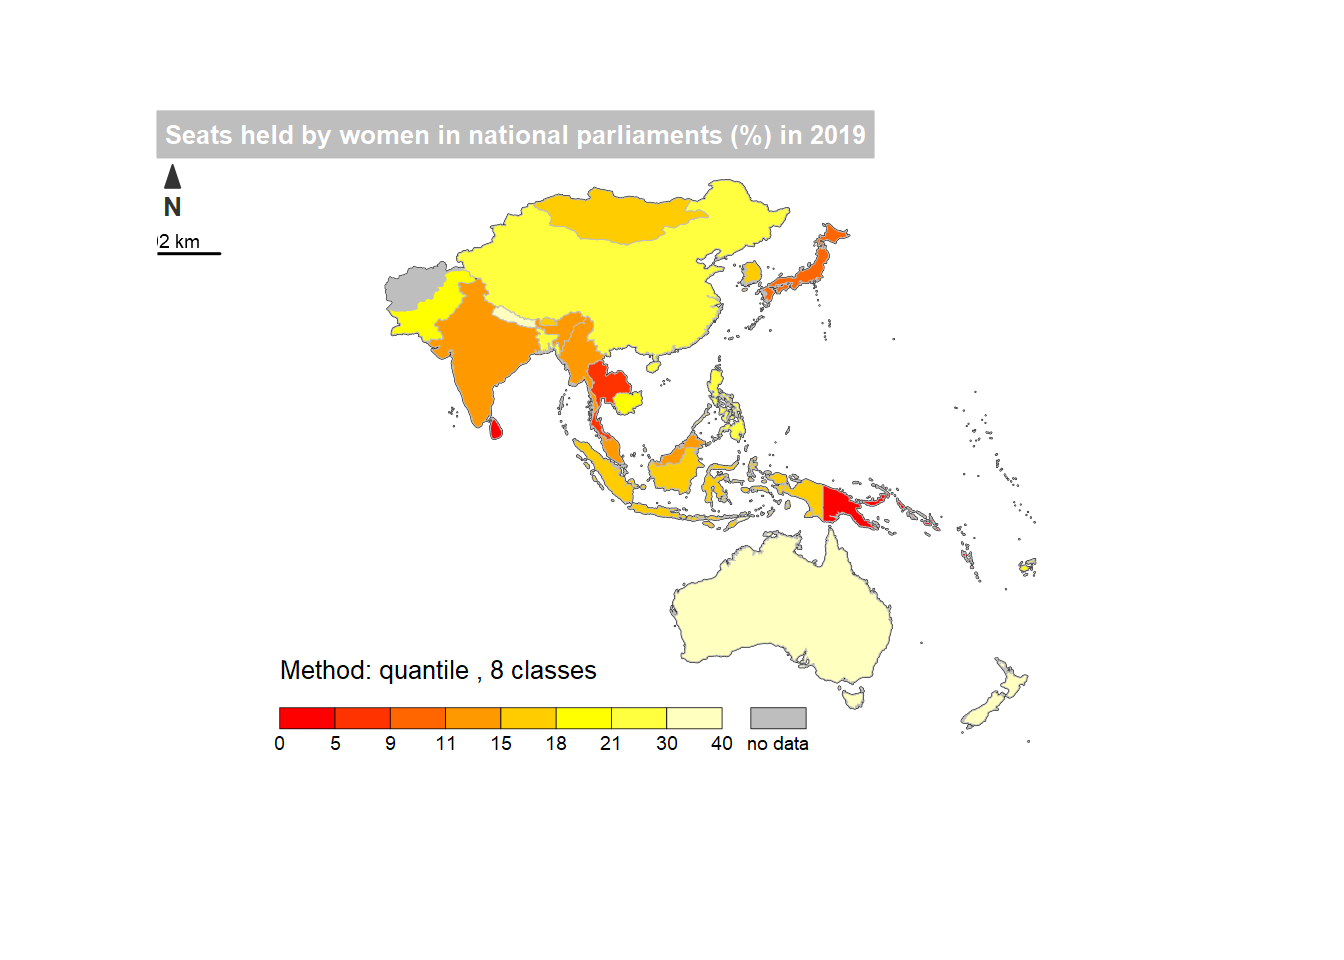
\includegraphics[width =0.9\textwidth]{BubbleMapChoropleth.png} }
    \only<2>{ 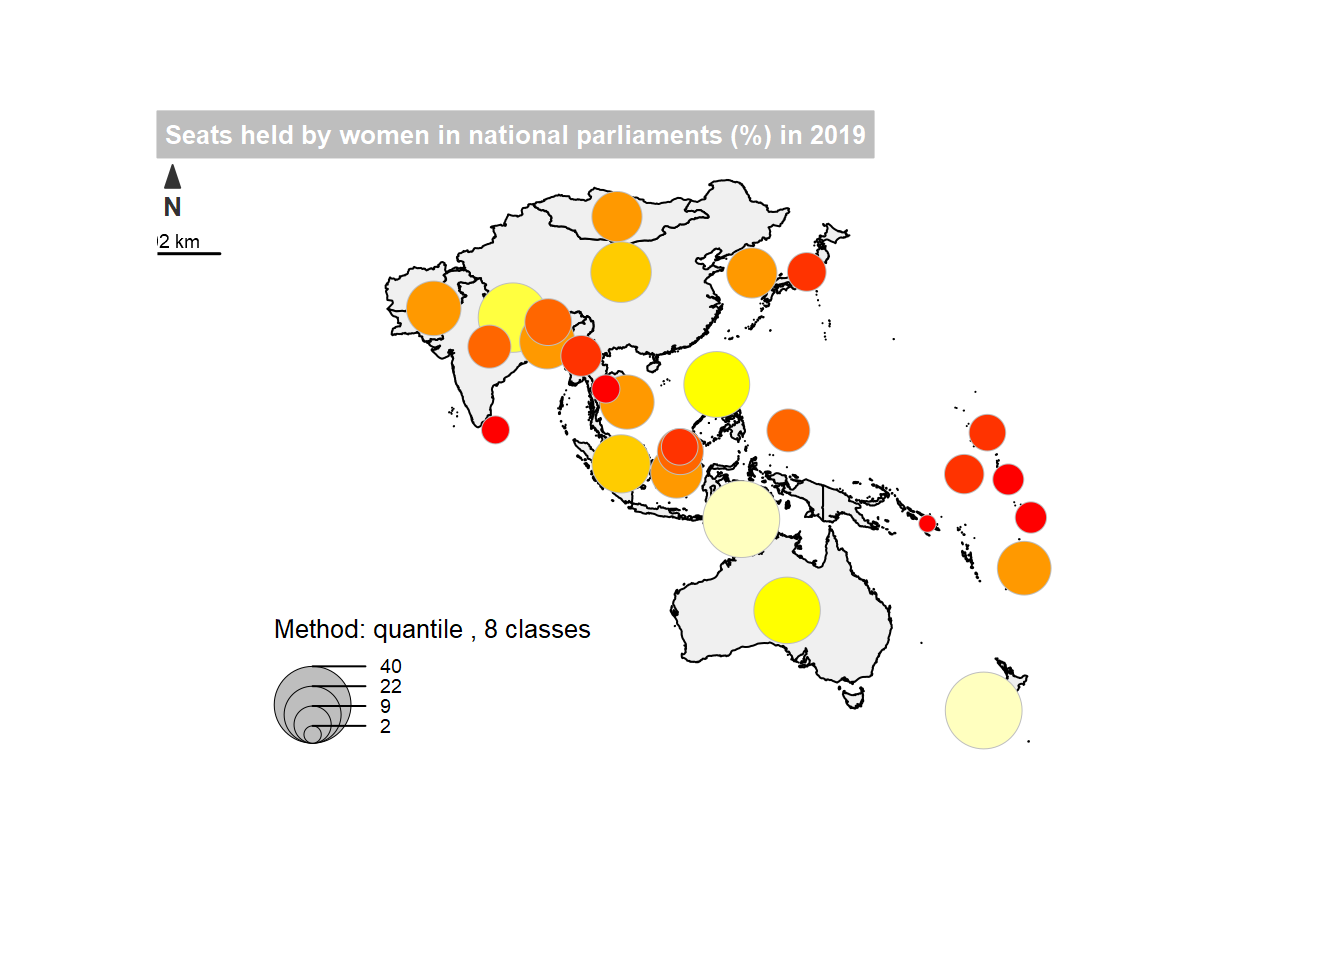
\includegraphics[width =0.9\textwidth]{BubbleMap.png} }
    \only<3>{ 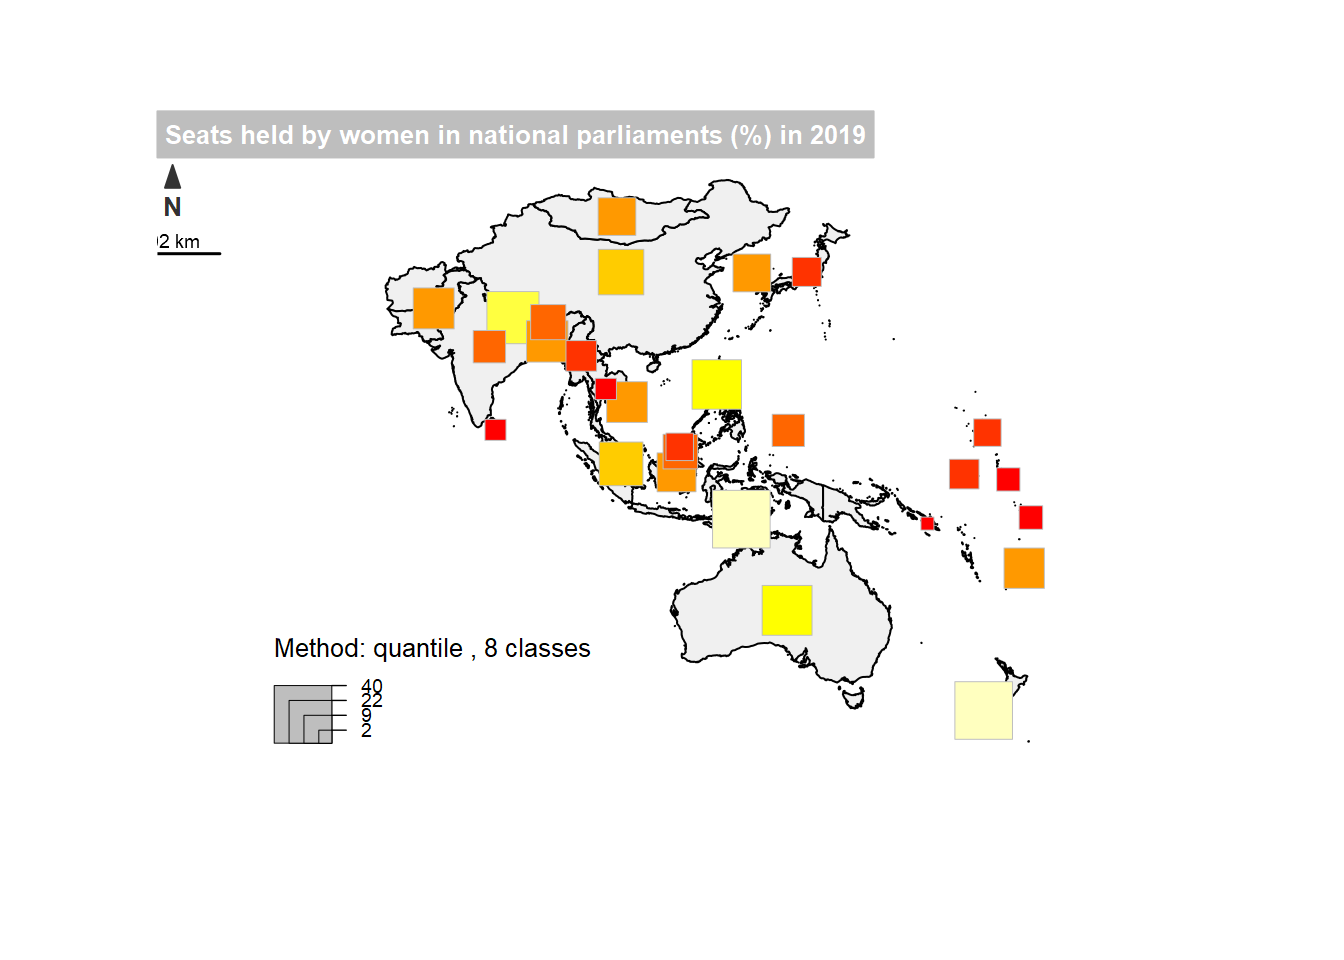
\includegraphics[width =0.9\textwidth]{BubbleMapSquares.png} }
    \only<4>{ 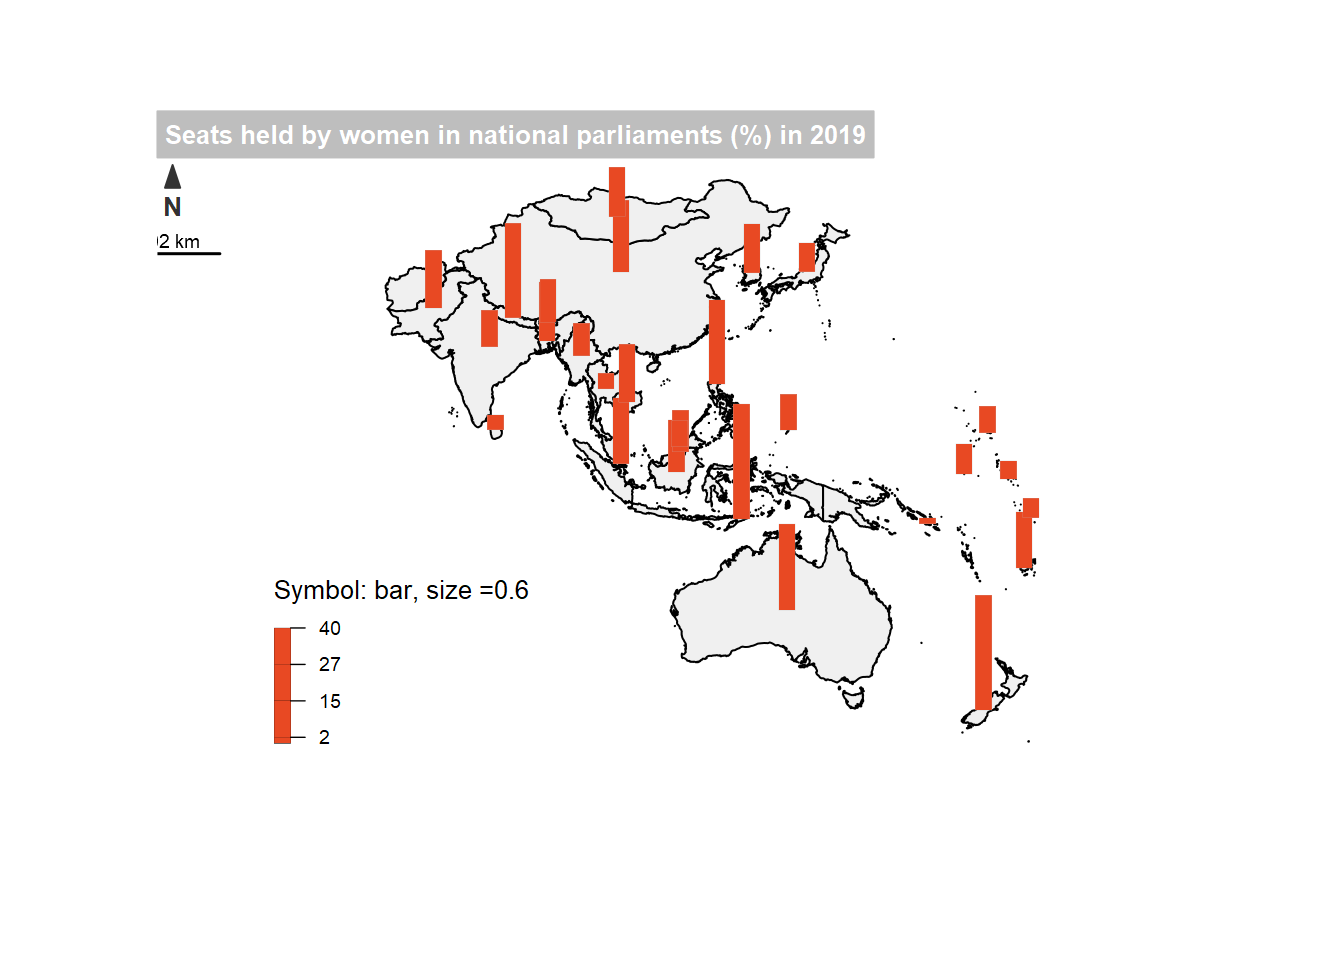
\includegraphics[width =0.9\textwidth]{BubbleMapBars.png} }
    \only<5>{ 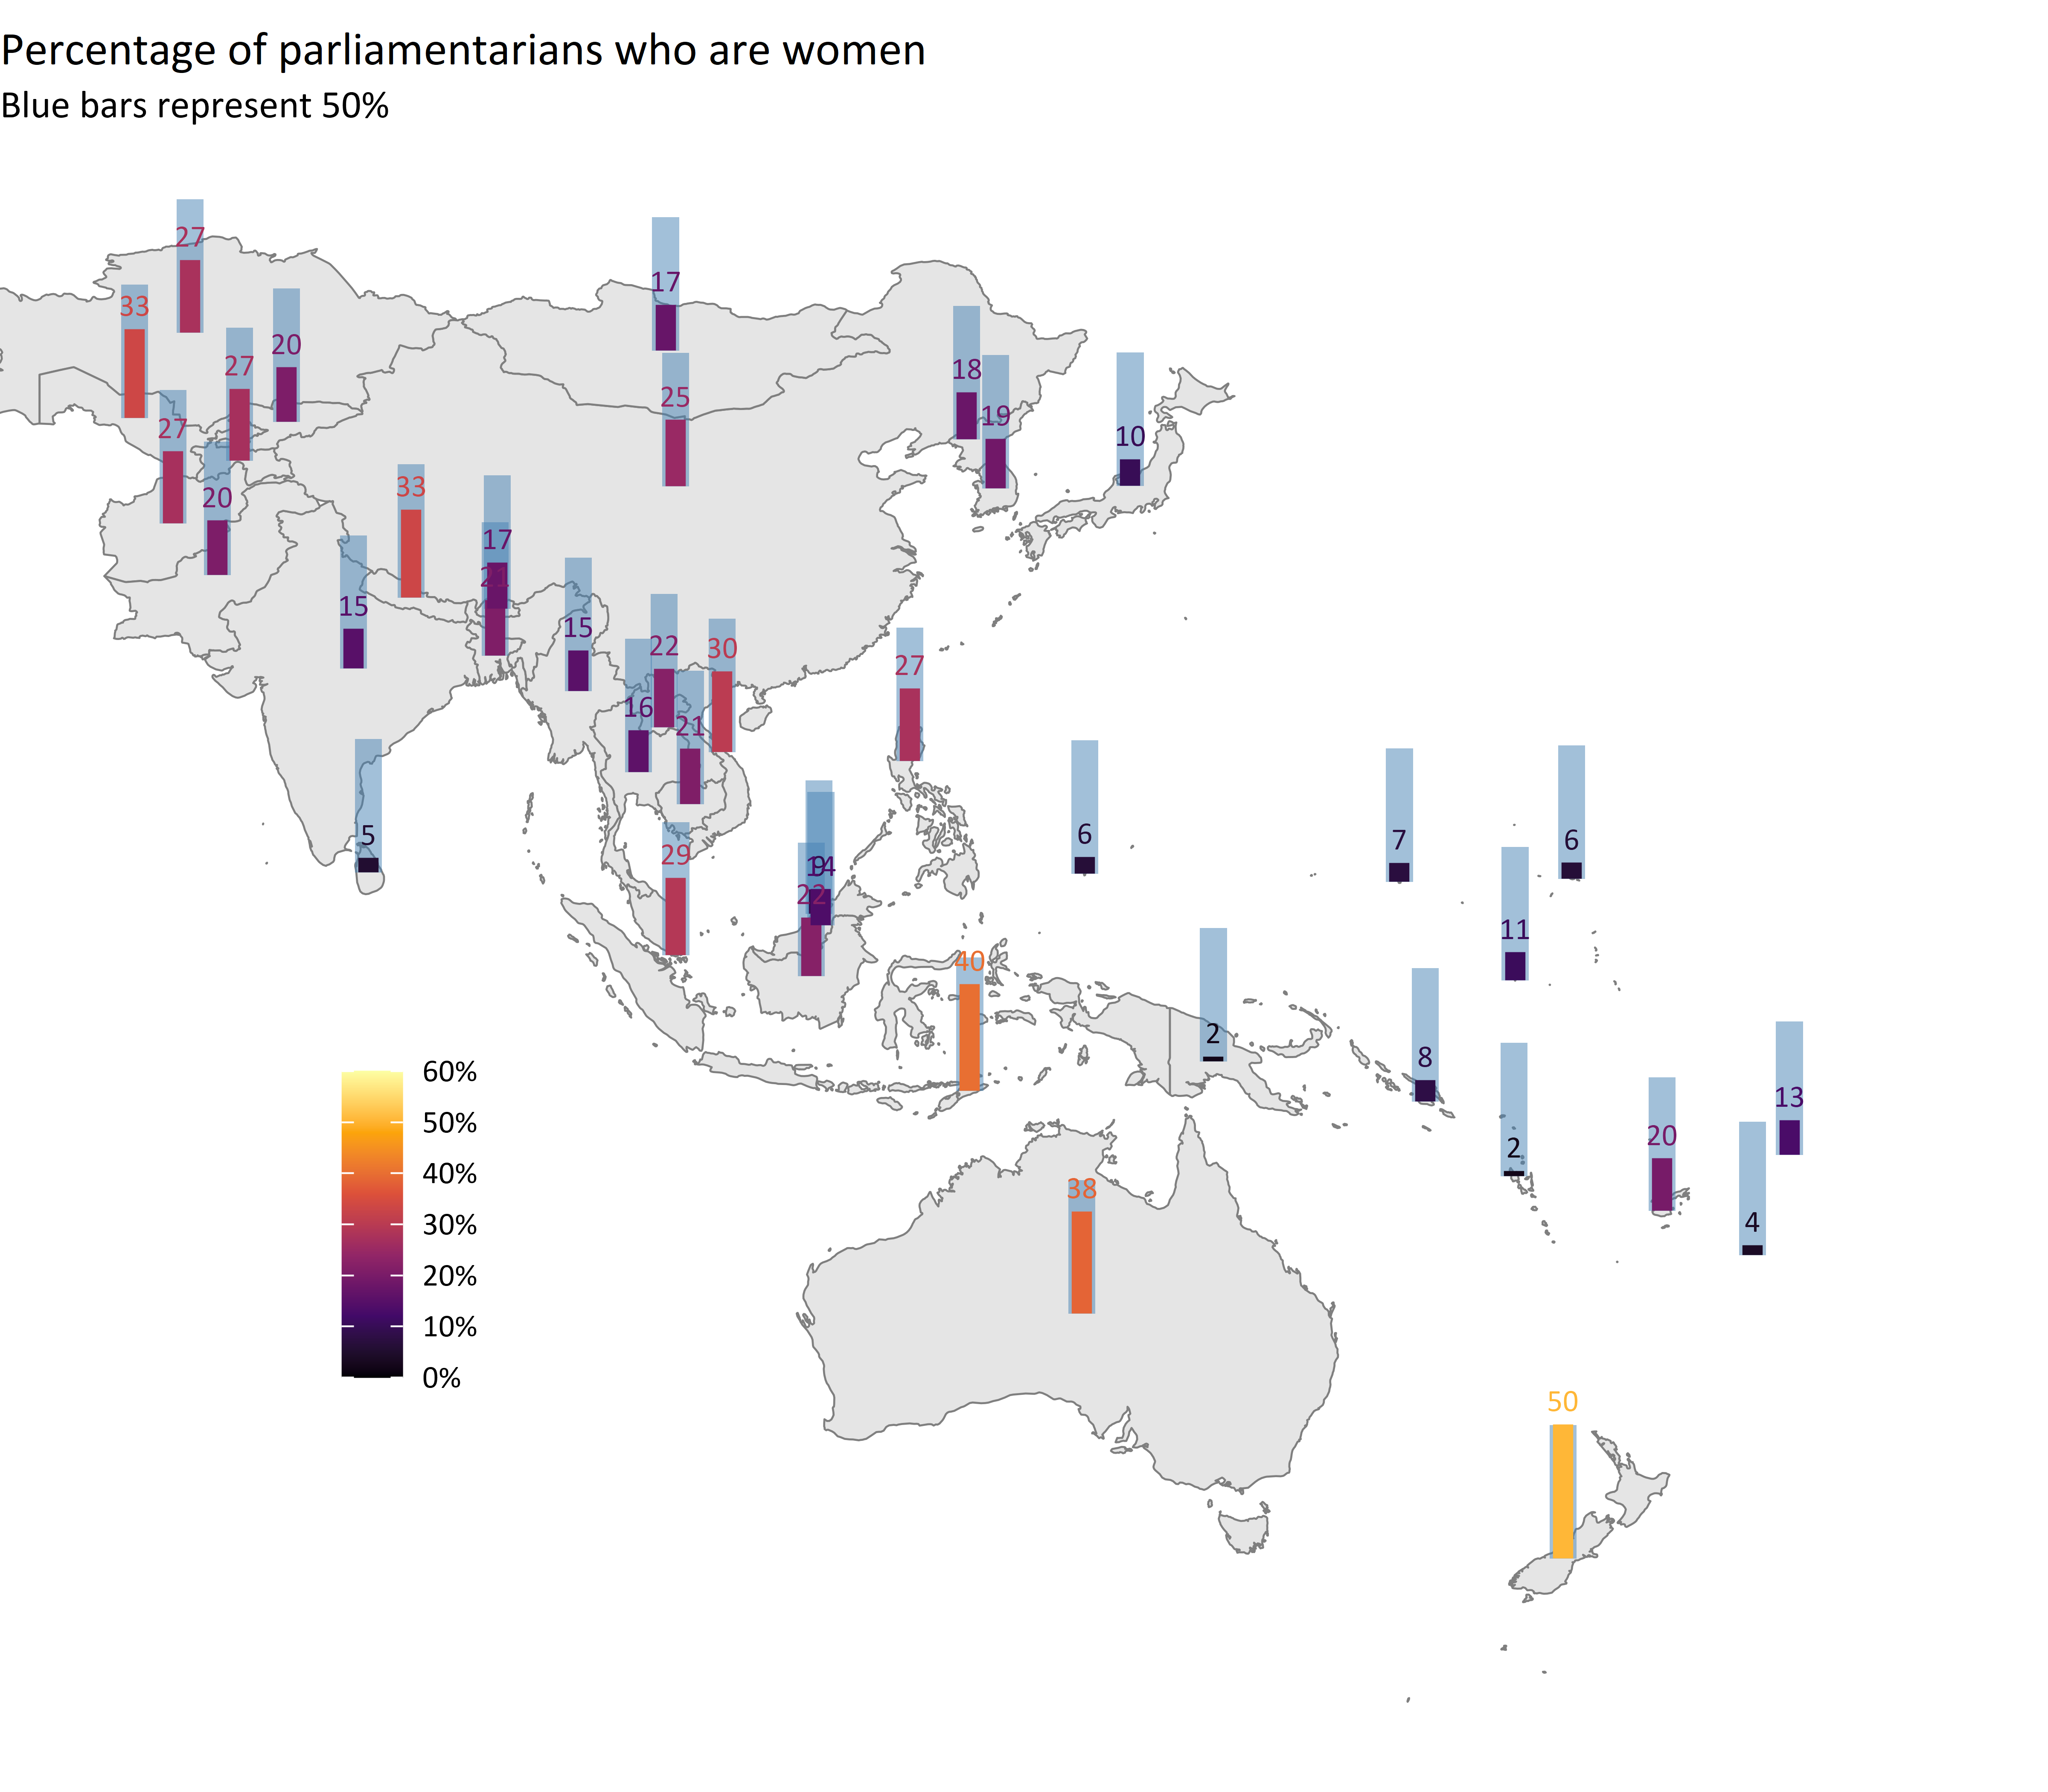
\includegraphics[width =0.65\textwidth]{PEllisGaugeMap.png} }

\end{itemize}
\end{center}
\end{frame}

%
%\section{Good lies}
%
%\begin{frame}
%\frametitle{\textcolor{airforceblue}{[- \textbf{Lying for a good reason} -]}}
%
%There are many visualisation that transform the data for clarity: \textbf{Subway maps} for example
%\begin{center}
%\begin{itemize}
% \item[]
%\only<1>{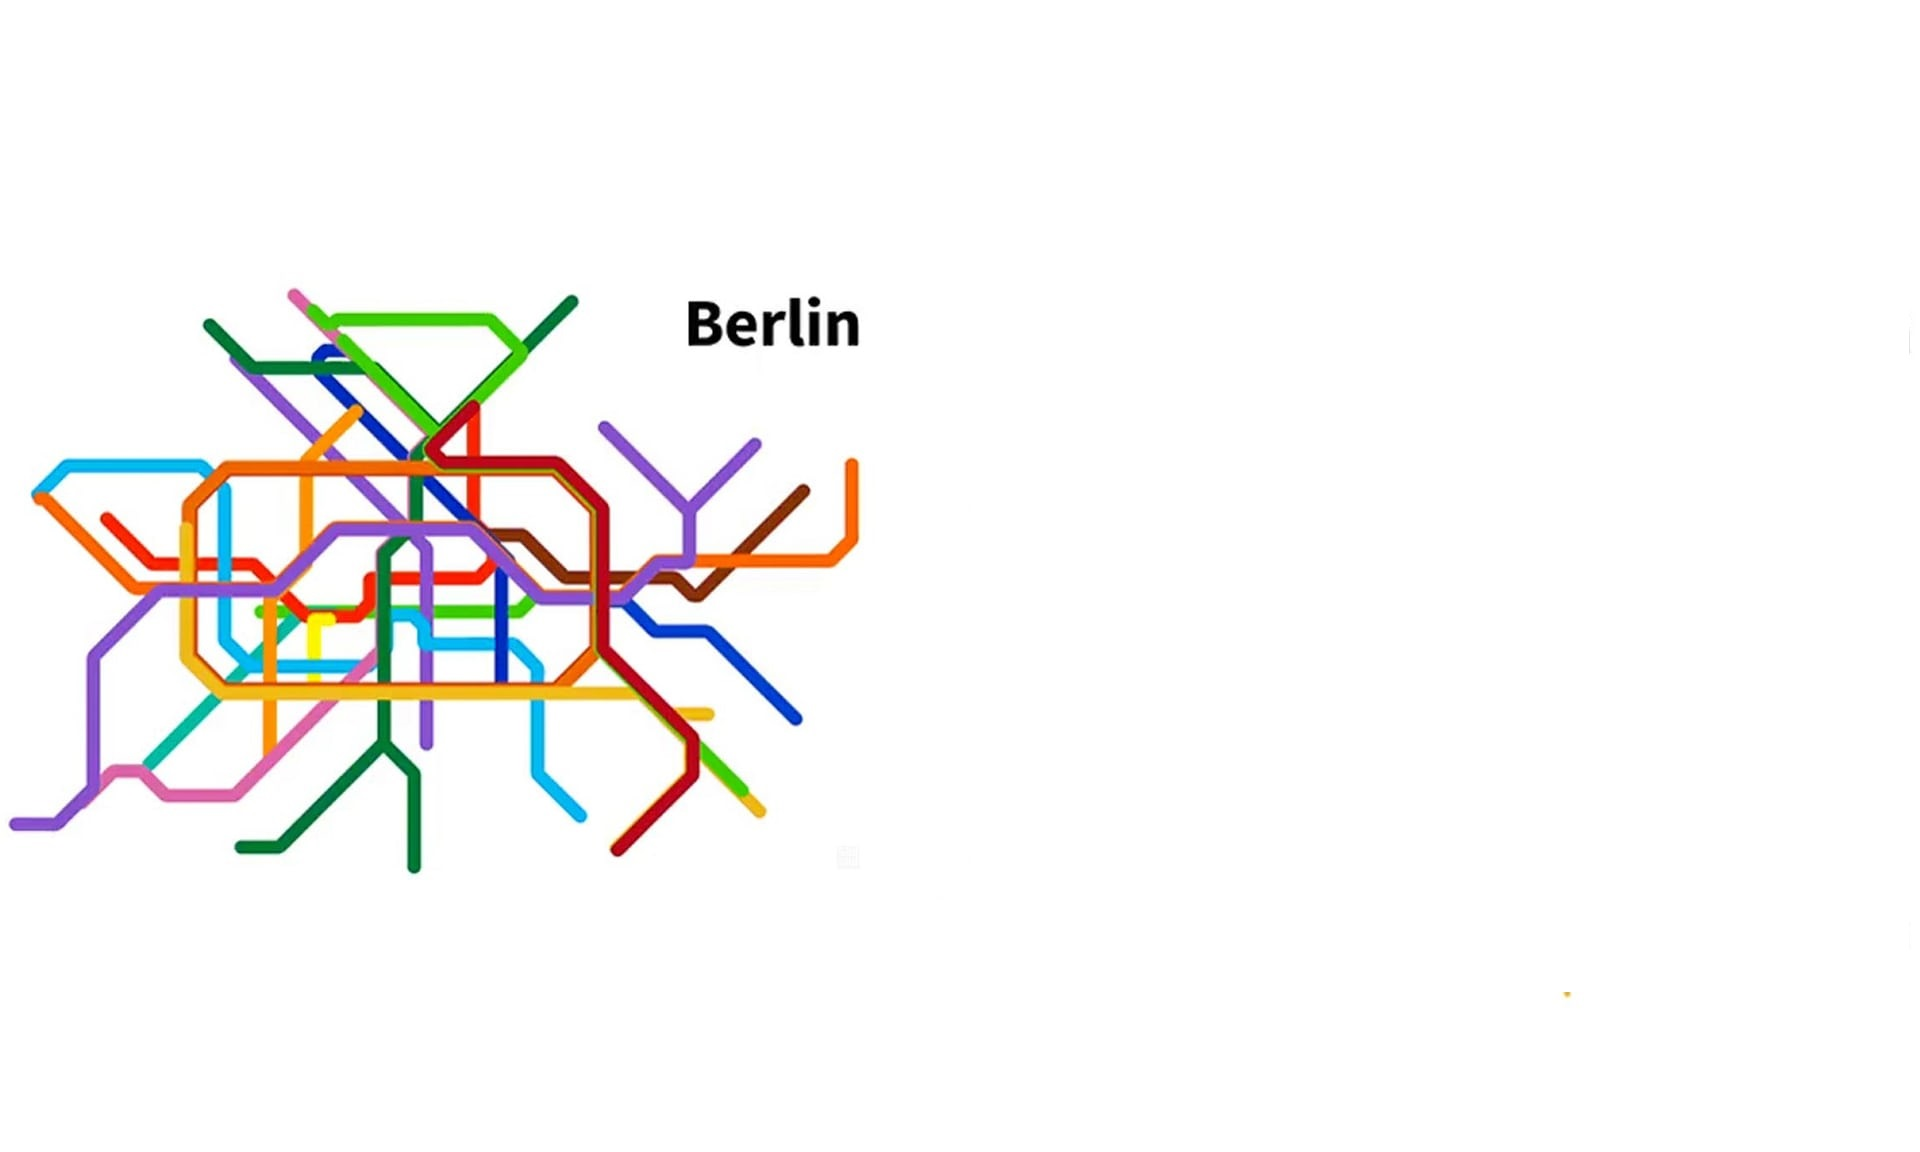
\includegraphics[width = 0.8\textwidth]{BerlinSubwayMap.JPG}}
%\only<2>{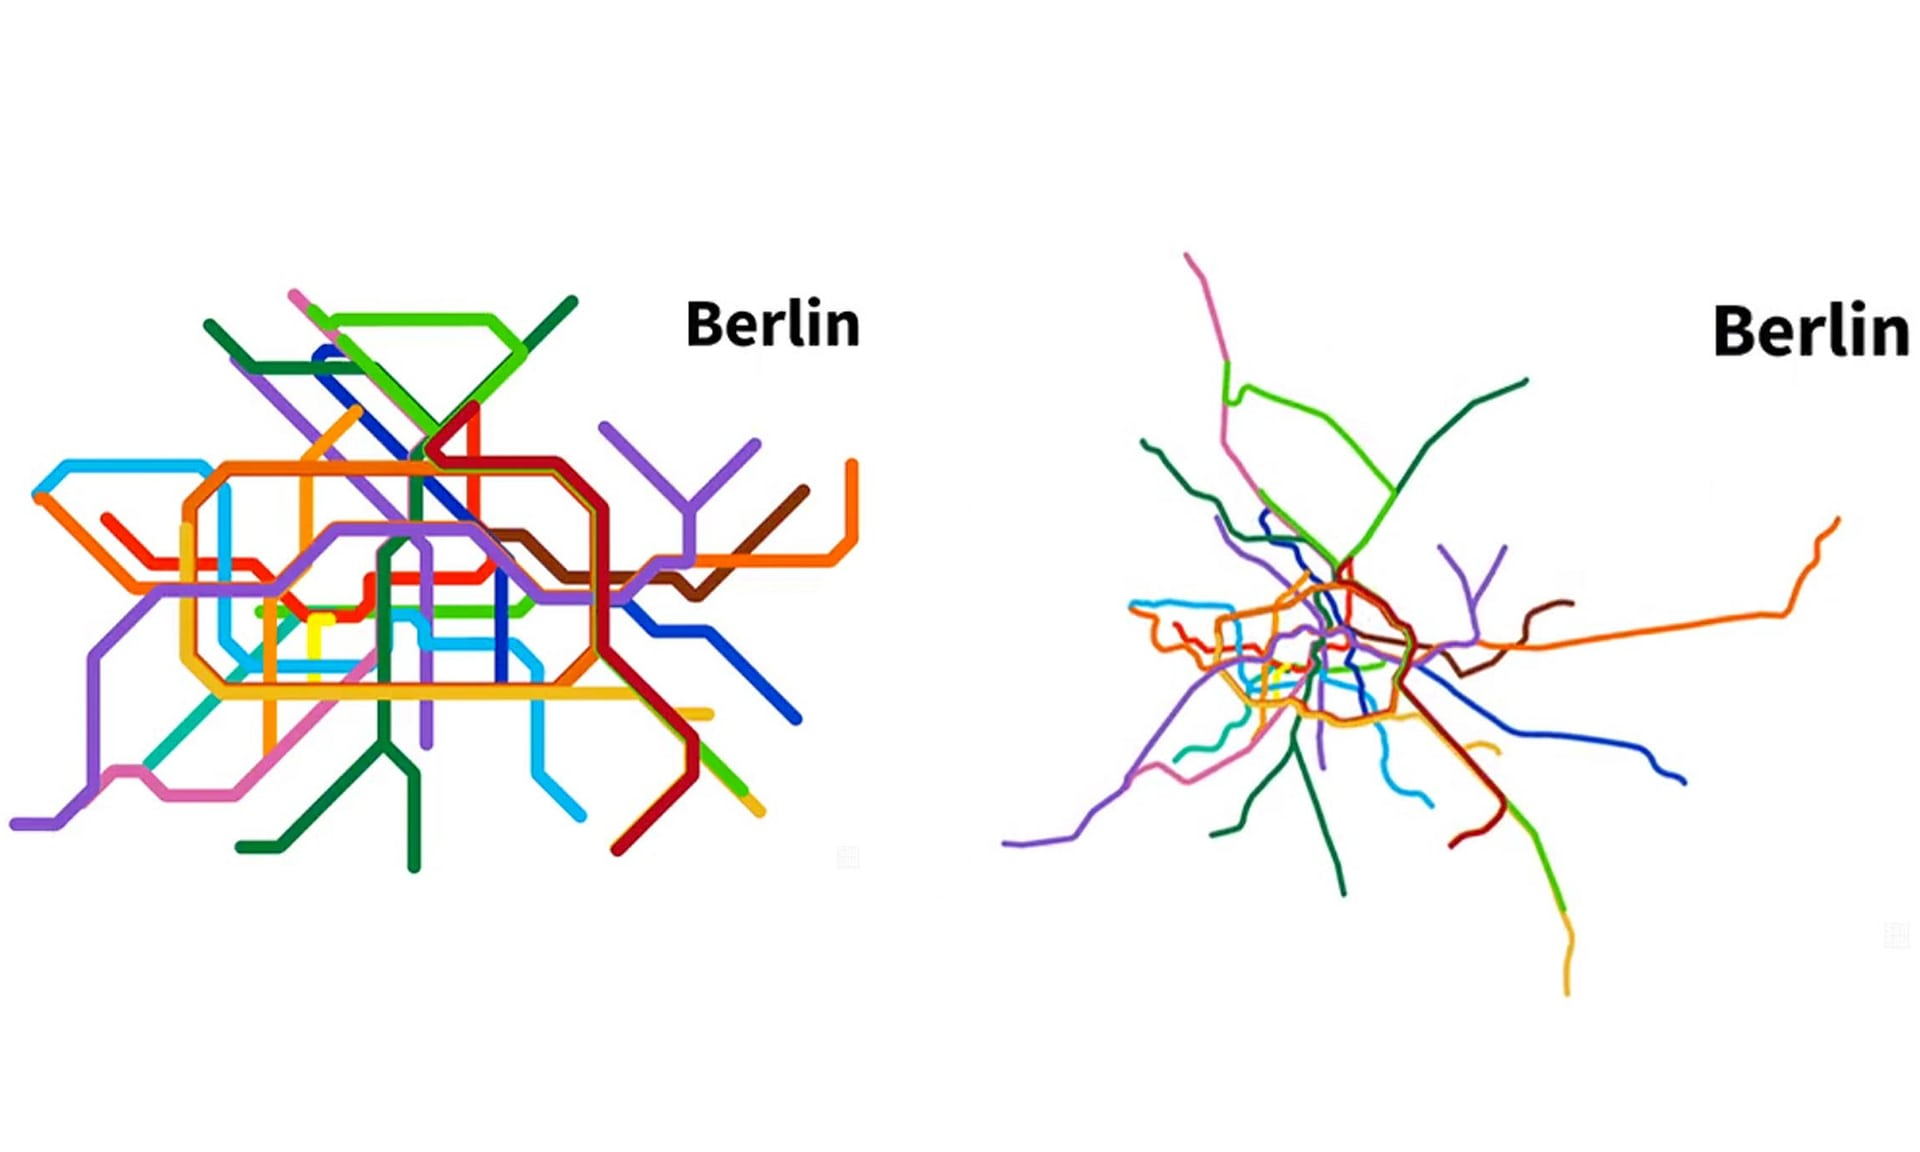
\includegraphics[width = 0.8\textwidth]{BerlinSubway.jpg}}
%\end{itemize}
%\end{center}
%
%\footnotesize{\textcolor{gris}{Source \href{https://www.theguardian.com/cities/2017/jun/27/twisted-tracks-metro-maps-real-life-geography-visualised
%}{The Guardian}}}
%\end{frame}
%
%\begin{frame}
%\frametitle{\textcolor{airforceblue}{[- \textbf{Lying for a good reason} -]}}
%\textbf{Subway maps} that match the physical reality are quite rare
%\begin{center}
%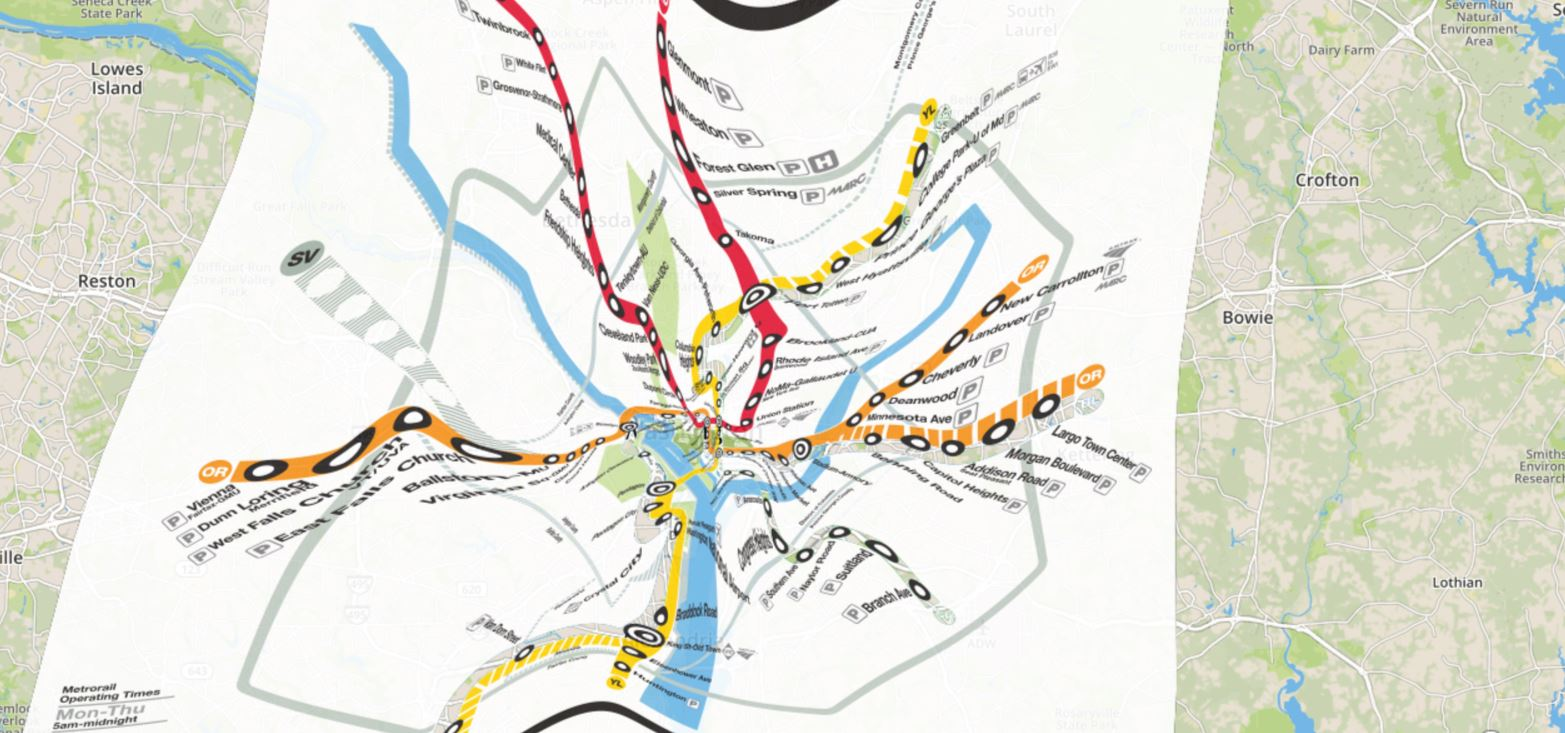
\includegraphics[width = 0.8\textwidth]{PhysicalSubway.JPG}
%\end{center}
%\footnotesize{\textcolor{gris}{Source \href{http://benschmidt.org/dcmetro/}{Benjamin Schmidt }}}
%\end{frame}

%
%\begin{frame}
%\frametitle{\textcolor{airforceblue}{[- \textbf{Lying for a good reason} -]}}
%\textbf{Ski resort maps} %are also neither maps, nor pictures, nor projections but paintings!
%\begin{center}
%\includegraphics[width = 0.8\textwidth]{12-Valloire-Plan-Pistes-NOVAT.jpg}
%\end{center}
%\footnotesize{\textcolor{gris}{Source \href{http://atelier.novat.free.fr/atelier_pierre_novat/accueil.html}{Pierre Novat }}}
%
%%We are here in the realm of an artist representation of a printed landscape showing both south, east and north-oriented slopes....
%\end{frame}
%
%
\section{Conclusion}

\begin{frame}
\frametitle{\textcolor{airforceblue}{Famous last words}}


\begin{center}
\begin{itemize}
   \item<+->[] \Large{\textit{"Data don't Lie."}}
   \item<+->[]\Large{\textit{"Statistics don't Lie."}}
   \item<+->[]\Large{\textit{"Graphics don't Lie."}}
   \item<+->[]
   \item<+->[]\Large{\textit{"People do..."}}
   \item<+->[]

\end{itemize}
\end{center}
\end{frame}

%\section{Thanks}


\begin{frame}
\frametitle{\textcolor{airforceblue}{[- \textbf{Comforting lies...} -]}}
\begin{center}
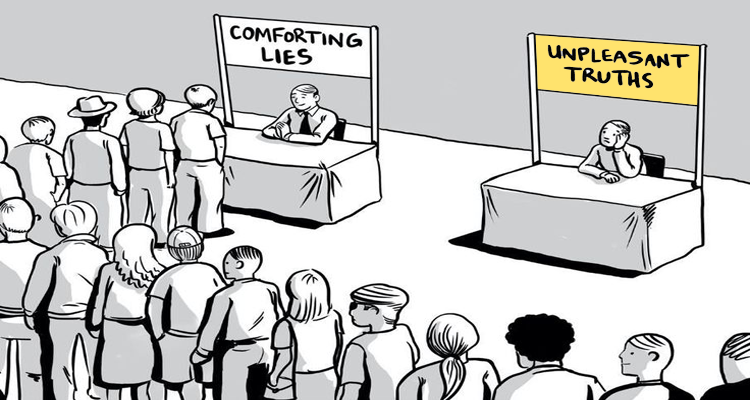
\includegraphics[width = 0.8\textwidth]{War-on-Cash-for-Digital-Ledger-Dreamers-vs-Metalheads-Liberty.png} \\

%
\includegraphics[height=0.5cm]{TwitterLogoNew.png} \emph{\color{twitterblue}{ @Xtophe\_Bontemps}} \\
%\url{http://data.visualisation.free.fr}

\end{center}
\end{frame}




\begin{frame}
\frametitle{\textcolor{brique}{[- \textbf{SIAP's Courses}]}}
Check \textcolor{siap}{\href{https://siap-elearning.org/course/view.php?id=124}{SIAP's Data Visualization courses}}
\begin{center}

\includegraphics[width = 0.20\textwidth]{SIAP_DTV_S.PNG}
\end{center}
Link to \textcolor{siap}{\footnotesize{\href{https://siap-elearning.org/course/view.php?id=124}{SIAP's Data Visualization (self-paced) }}}
\end{frame}





%%%%%%%%%%%%%%% Last Slide %%%%%%%%%%%%%%%%

\begin{frame}[allowframebreaks]%in case more than 1 slide needed
\frametitle{References}
\begin{center}

\includegraphics[width = 0.6\textwidth]{Bibliography.jpg}
\end{center}

%\nocite{Cairo2019}
%\nocite{Correll2019}
%\nocite{Allen2016}
%\nocite{Isenberg2011}
%\nocite{Kelleher2011}
%\nocite{Tufte2001}
%\nocite{Cleveland1982}
%\nocite{*}
    {\footnotesize
    %\bibliographystyle{authordate1}
    \bibliographystyle{apalike}
    \bibliography{Visu}
    }
\end{frame}

%\section{Thanks}

\end{document}

%%%%%%%%%%%%%%% ELECTION MAPS %%%%%%%%%%%%%%%%%%%%%%%




\begin{frame} % Cover slide
\label{USAMAPS}
\frametitle{\textcolor{brique}{[- \textbf{Super Rule \#3: Use Electoral Maps} -]}}
USA election: \textbf{2016} results as a map: \href{https://www.washingtonpost.com/news/the-fix/wp/2016/12/14/why-democrats-need-to-spend-less-time-worrying-about-the-presidential-race/?postshare=7251481738295298&tid=ss_tw&utm_term=.1314a25ee261}{
Washington Post}
\begin{center}
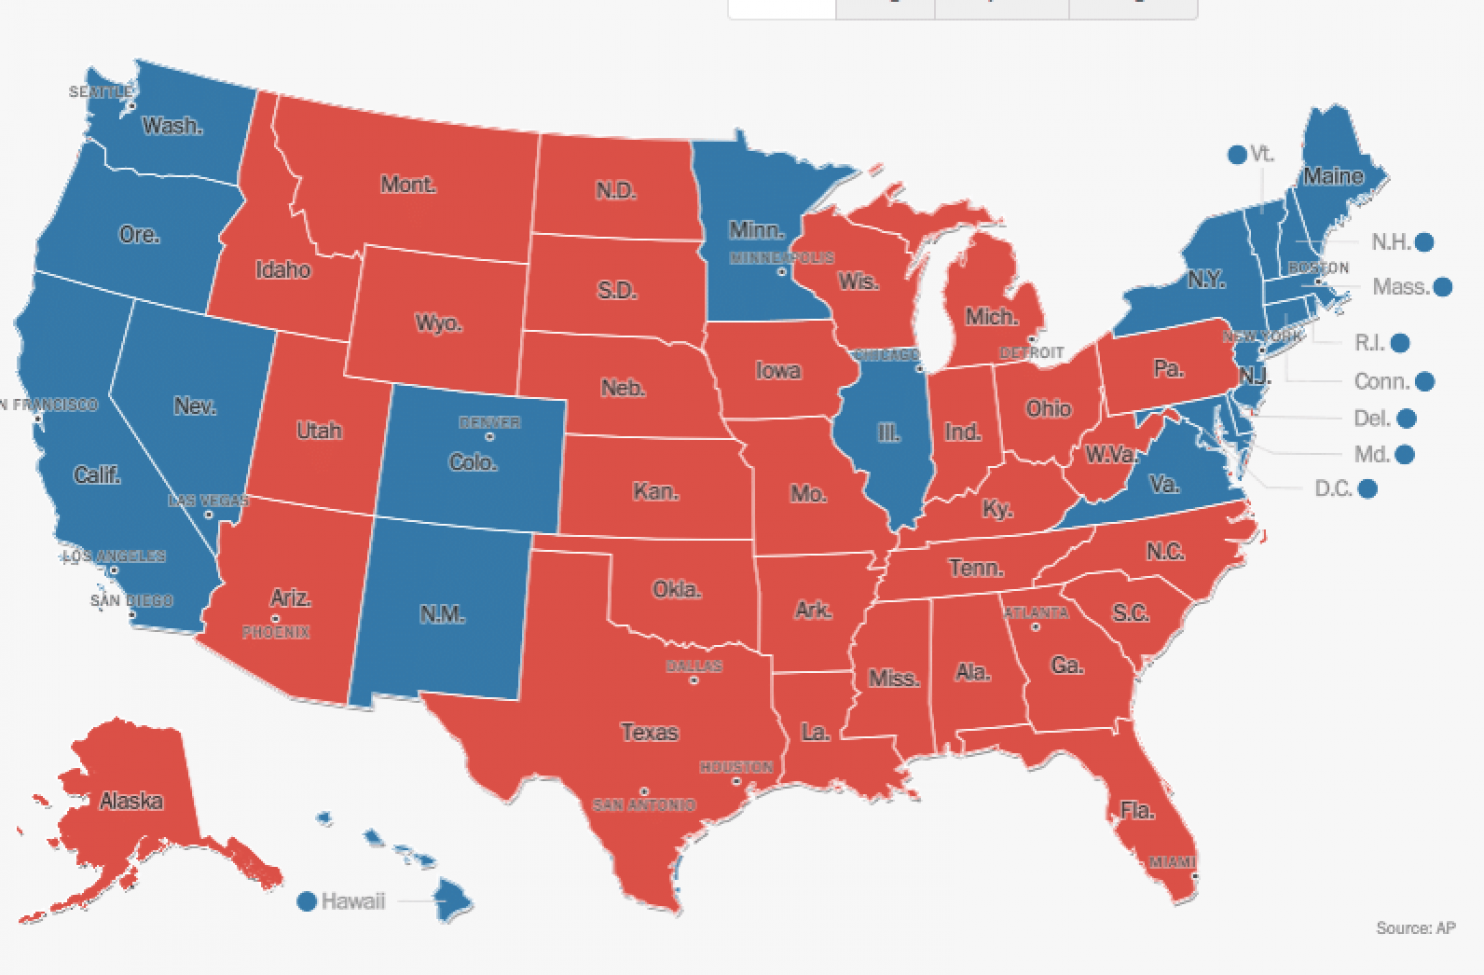
\includegraphics[width=1.02\textwidth]{USElectionNYT2016.png}
\end{center}
\end{frame}


\begin{frame} % Cover slide
\label{USAMAPS}
\frametitle{\textcolor{brique}{[- \textbf{Super Rule \#3: Use Electoral Maps} -]}}
USA election: \textbf{2012} results as a map: \href{https://www.nytimes.com/2016/09/09/upshot/red-states-blue-states-does-this-map-look-familiar.html}{
New York Time}
\begin{center}
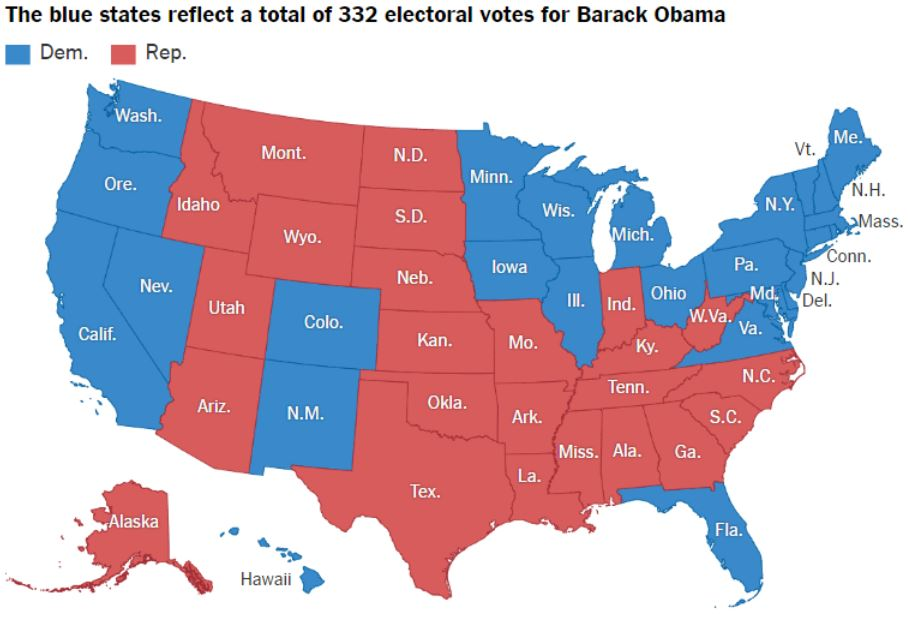
\includegraphics[width=1.0\textwidth]{USElectionNYT2012.JPG}
\end{center}
\end{frame}

\begin{frame} % Cover slide
\frametitle{\textcolor{brique}{[- \textbf{Super Rule \#3: Use Electoral Maps} -]}}
\label{USAMAPS}
USA election: \textbf{2008} results as a map: \href{https://www.nytimes.com/2016/09/09/upshot/red-states-blue-states-does-this-map-look-familiar.html}{
New York Time}
\begin{center}
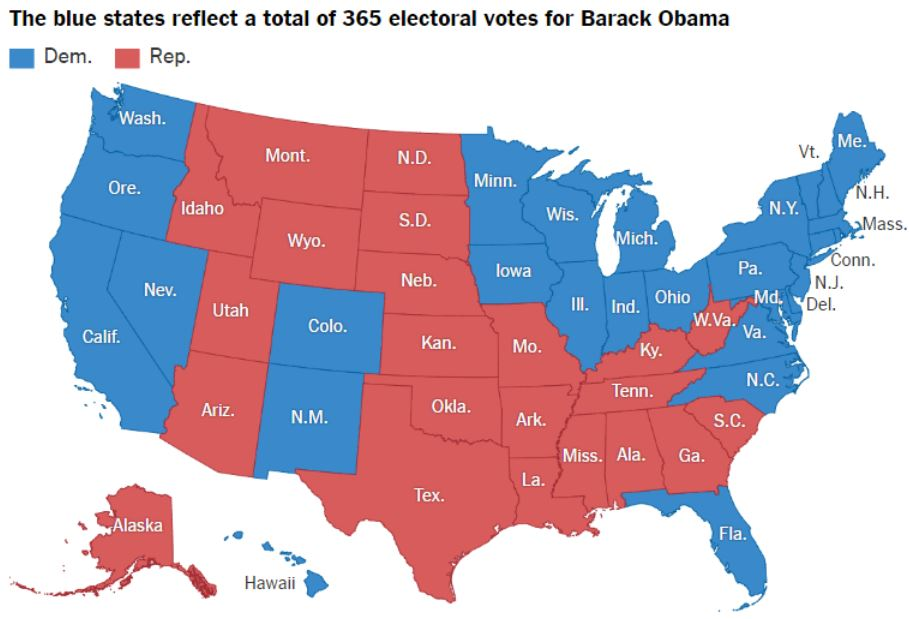
\includegraphics[width=1.0\textwidth]{USElectionNYT2008.JPG}
\end{center}
\end{frame}


\begin{frame} % Cover slide
\frametitle{\textcolor{brique}{[- \textbf{Super Rule \#3: Use Electoral Maps} -]}}
\label{USAMAPS}
Maybe a better map? From  \href{https://ig.ft.com/us-elections/results}{\textit{Financial Times blog }}
\begin{center}
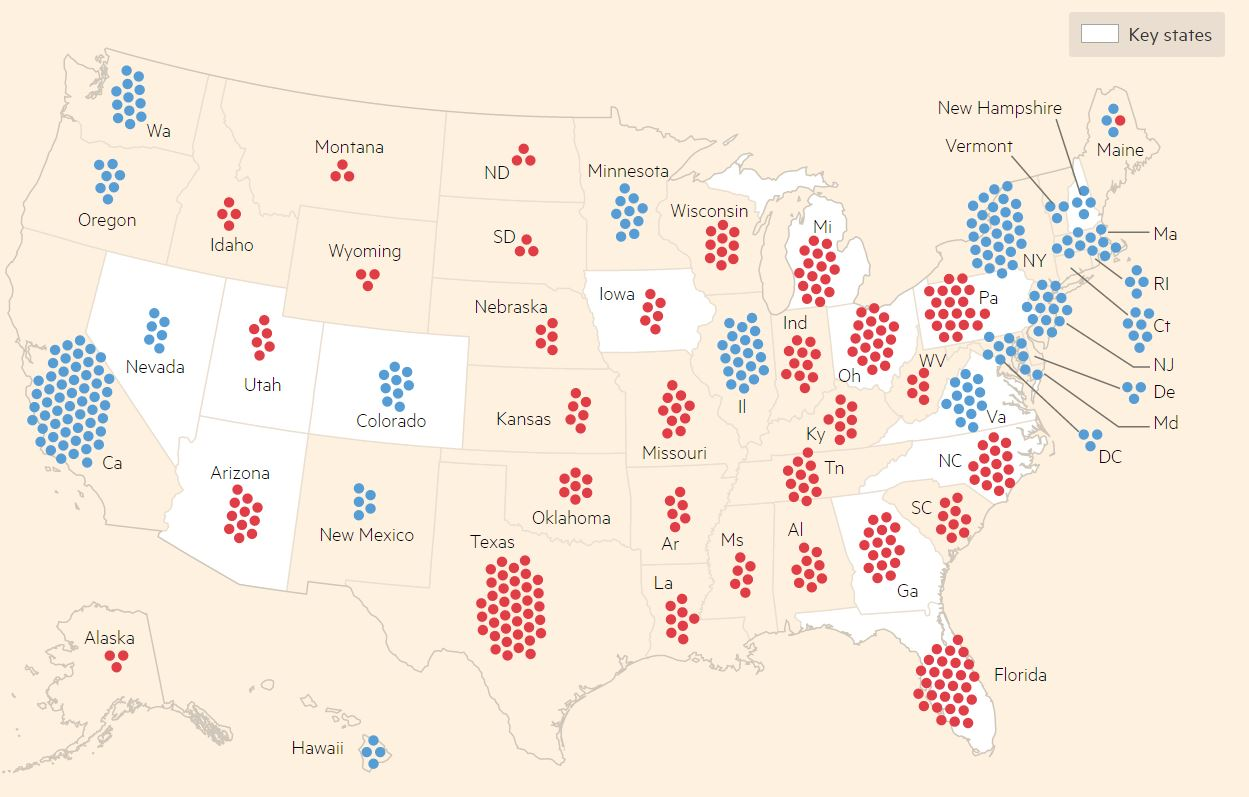
\includegraphics[width=0.9\textwidth]{US_election_dot_map2016.png}
\end{center}
From  \href{https://ig.ft.com/us-elections/results}{\textit{Financial Times}}
\end{frame}


\begin{frame} % Cover slide
\frametitle{\textcolor{brique}{[- \textbf{Super Rule \#3: Use Electoral Maps} -]}}
\label{USMAPS}
Maybe spatial information is not the most relevant!
\begin{center}
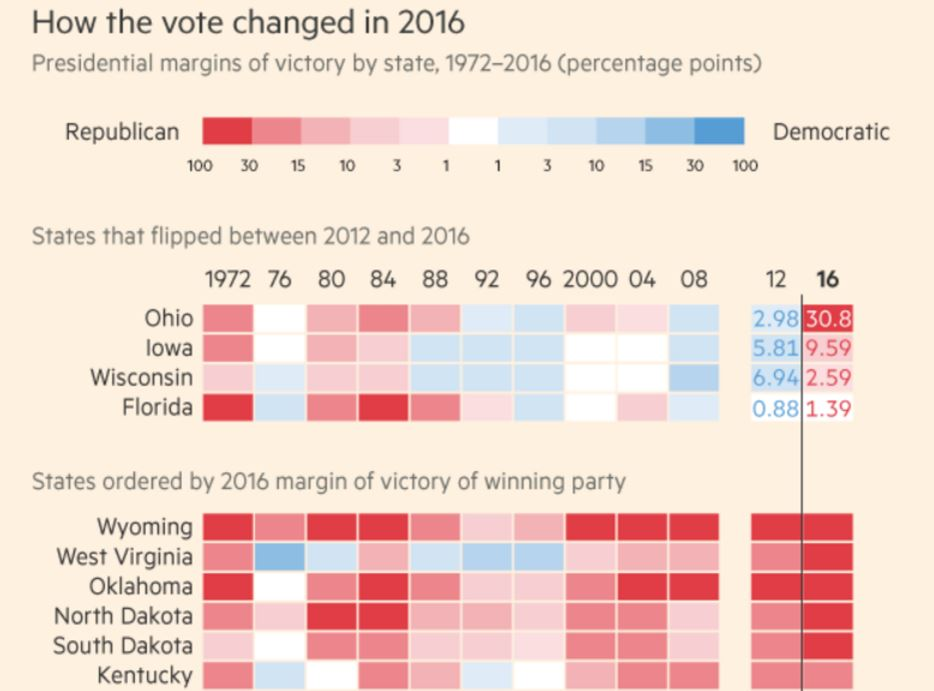
\includegraphics[width=1.0\textwidth]{USElectionChanges.JPG}
\end{center}
From  \href{http://blogs.ft.com/the-world/liveblogs/2016-11-08/}{Financial Times blog }
\end{frame}

\begin{frame} % Cover slide
\label{USAMAPS}
\frametitle{\textcolor{brique}{[- \textbf{Super Rule \#3: Use Electoral Maps} -]}}
Maybe spatial information is not the most relevant!
\begin{center}
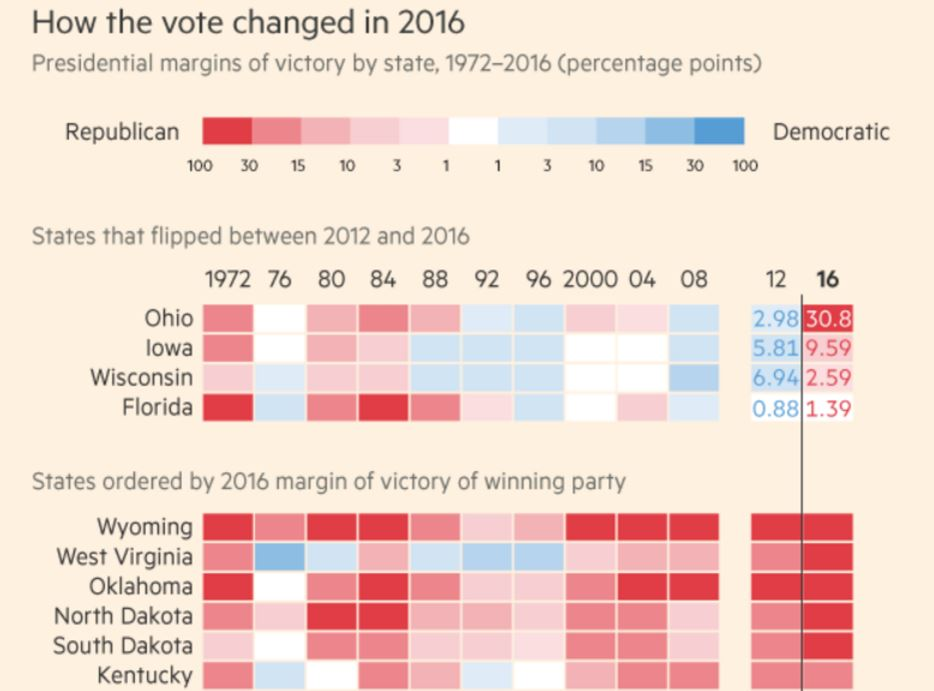
\includegraphics[width=0.4\textwidth]{USElectionChanges.JPG}   \hspace{0.5cm} 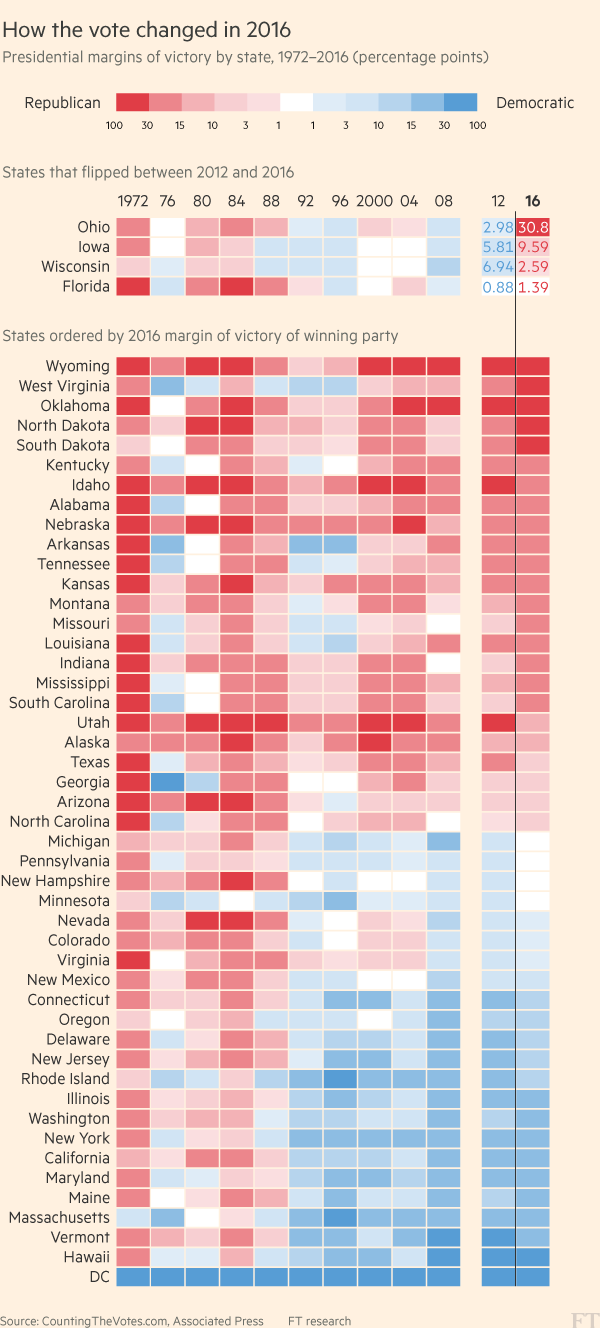
\includegraphics[width=0.3\textwidth]{Updated-what-happened.png}
\end{center}

From  \href{http://blogs.ft.com/the-world/liveblogs/2016-11-08/}{Financial Times blog}
\end{frame}



%%%%%%%%%%%%%%%%%%%%%%%%%%%%%%%%%%%%%%%% Dessinez  %%%%%%%%%%%%%%%%%%%%%%%%%
%\section{Tromper}

\begin{frame}
\frametitle{\textcolor{brique}{[- DIY -]}}
\begin{center}
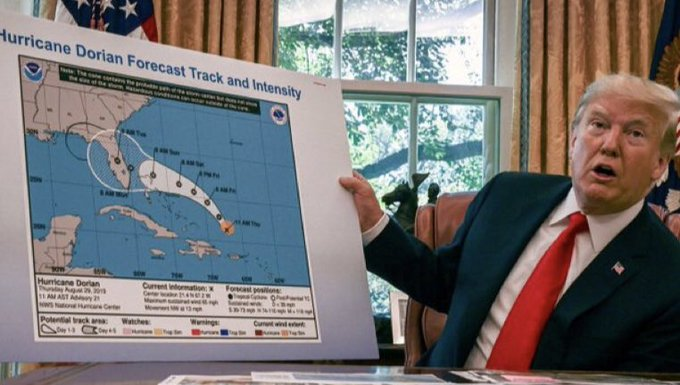
\includegraphics[width = 1.0\textwidth]{TrumpTornadoMap0.jpg}
\end{center}

\textcolor{gris}{\footnotesize{Source: \href{https://www.washingtonpost.com/opinions/2019/09/05/not-just-sharpie-gate-other-times-officials-tried-fabricate-trumps-truth/}{Washington Post }}}
\end{frame}

\begin{frame}
\frametitle{\textcolor{brique}{[- DIY -]}}
\begin{center}
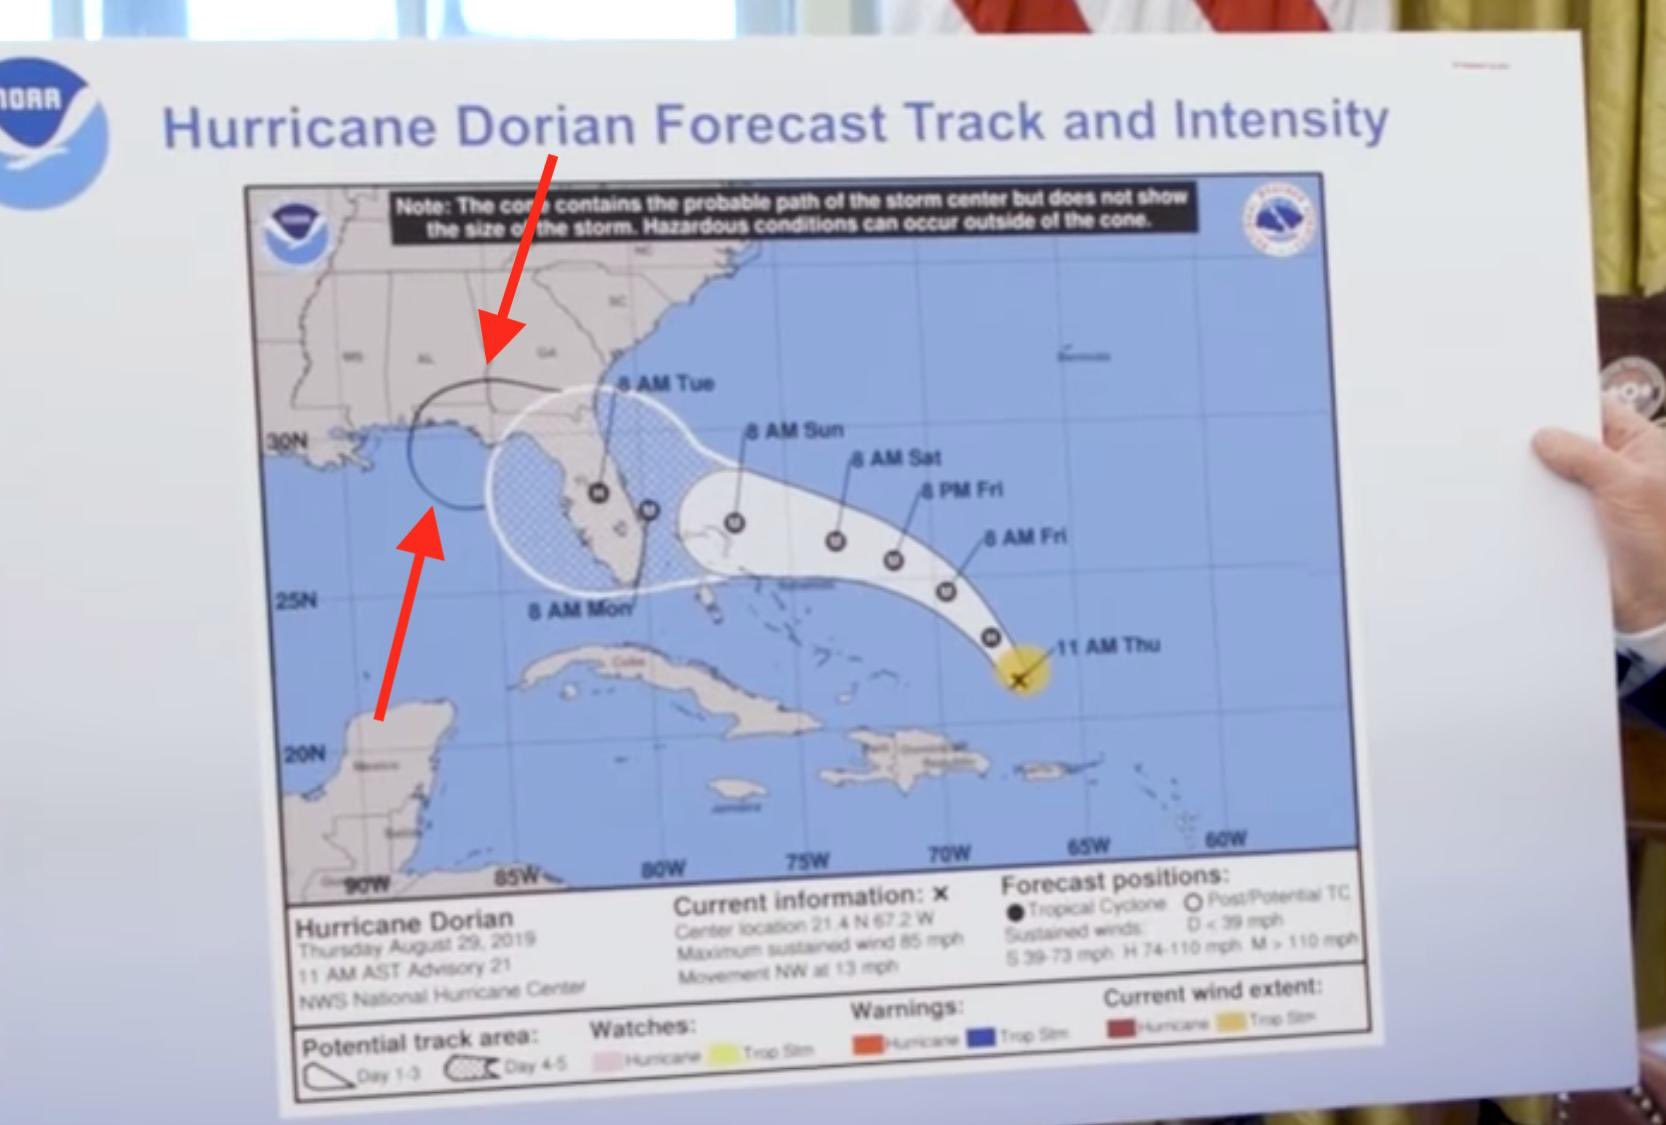
\includegraphics[width = 1.1\textheight]{TrumpTornadoMap1.jpg}
\end{center}

\textcolor{gris}{\footnotesize{Source: \href{https://www.washingtonpost.com/opinions/2019/09/05/not-just-sharpie-gate-other-times-officials-tried-fabricate-trumps-truth/}{Washington Post }}}
\end{frame}

\begin{frame}
\frametitle{\textcolor{brique}{[- DIY -]}}
\begin{center}
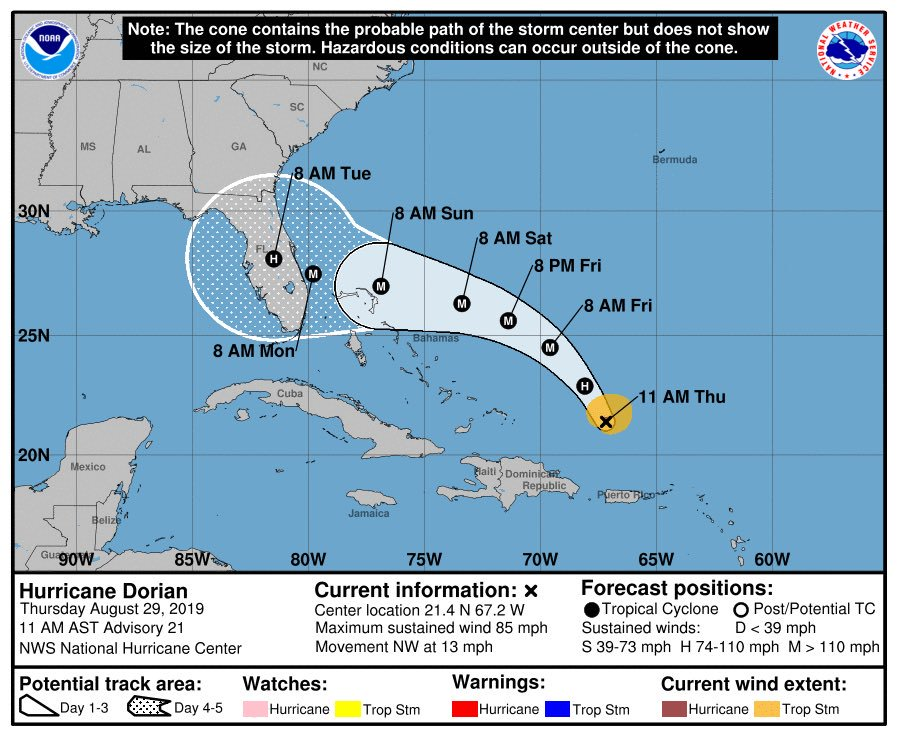
\includegraphics[width = 0.9\textheight]{TrumpTornadoMapReal.jpg}
\end{center}

\textcolor{gris}{\footnotesize{Source: \href{https://www.washingtonpost.com/opinions/2019/09/05/not-just-sharpie-gate-other-times-officials-tried-fabricate-trumps-truth/}{Washington Post }}}
\end{frame}



%%%%%%%%%%%%%%%%%%%%%%% Soyez Subtil %%%%%%%%%%%%%%%%%%%%%%%%%%%%%%%%%%%%%%%%%%%%%%%

%% Barres Elections Européennes...
\begin{frame}
\frametitle{\textcolor{brique}{[- Be Subtle -]}}
\begin{center}
\begin{enumerate}
   \only<1>{Original}
   \only<1>{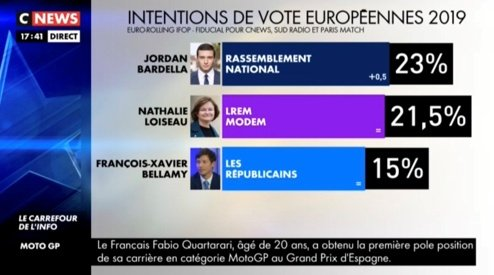
\includegraphics[width = 1.0\textwidth]{BarsElectionsLCI.jpg}}
   \only<2>{Corrigé}
   \only<2>{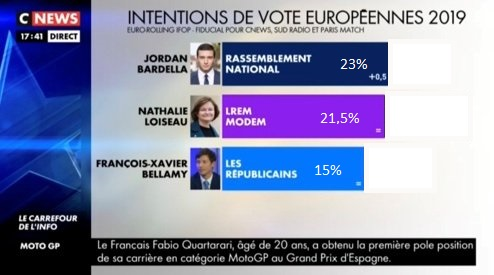
\includegraphics[width = 1.0\textwidth]{BarsElectionsLCIModif.jpg}}\\
\end{enumerate}
\end{center}
\end{frame}


%% Barres macron
\begin{frame}
\frametitle{\textcolor{brique}{[- Be Subtle -]}}
\begin{center}
\begin{enumerate}
   \only<1>{Original}
   \only<1>{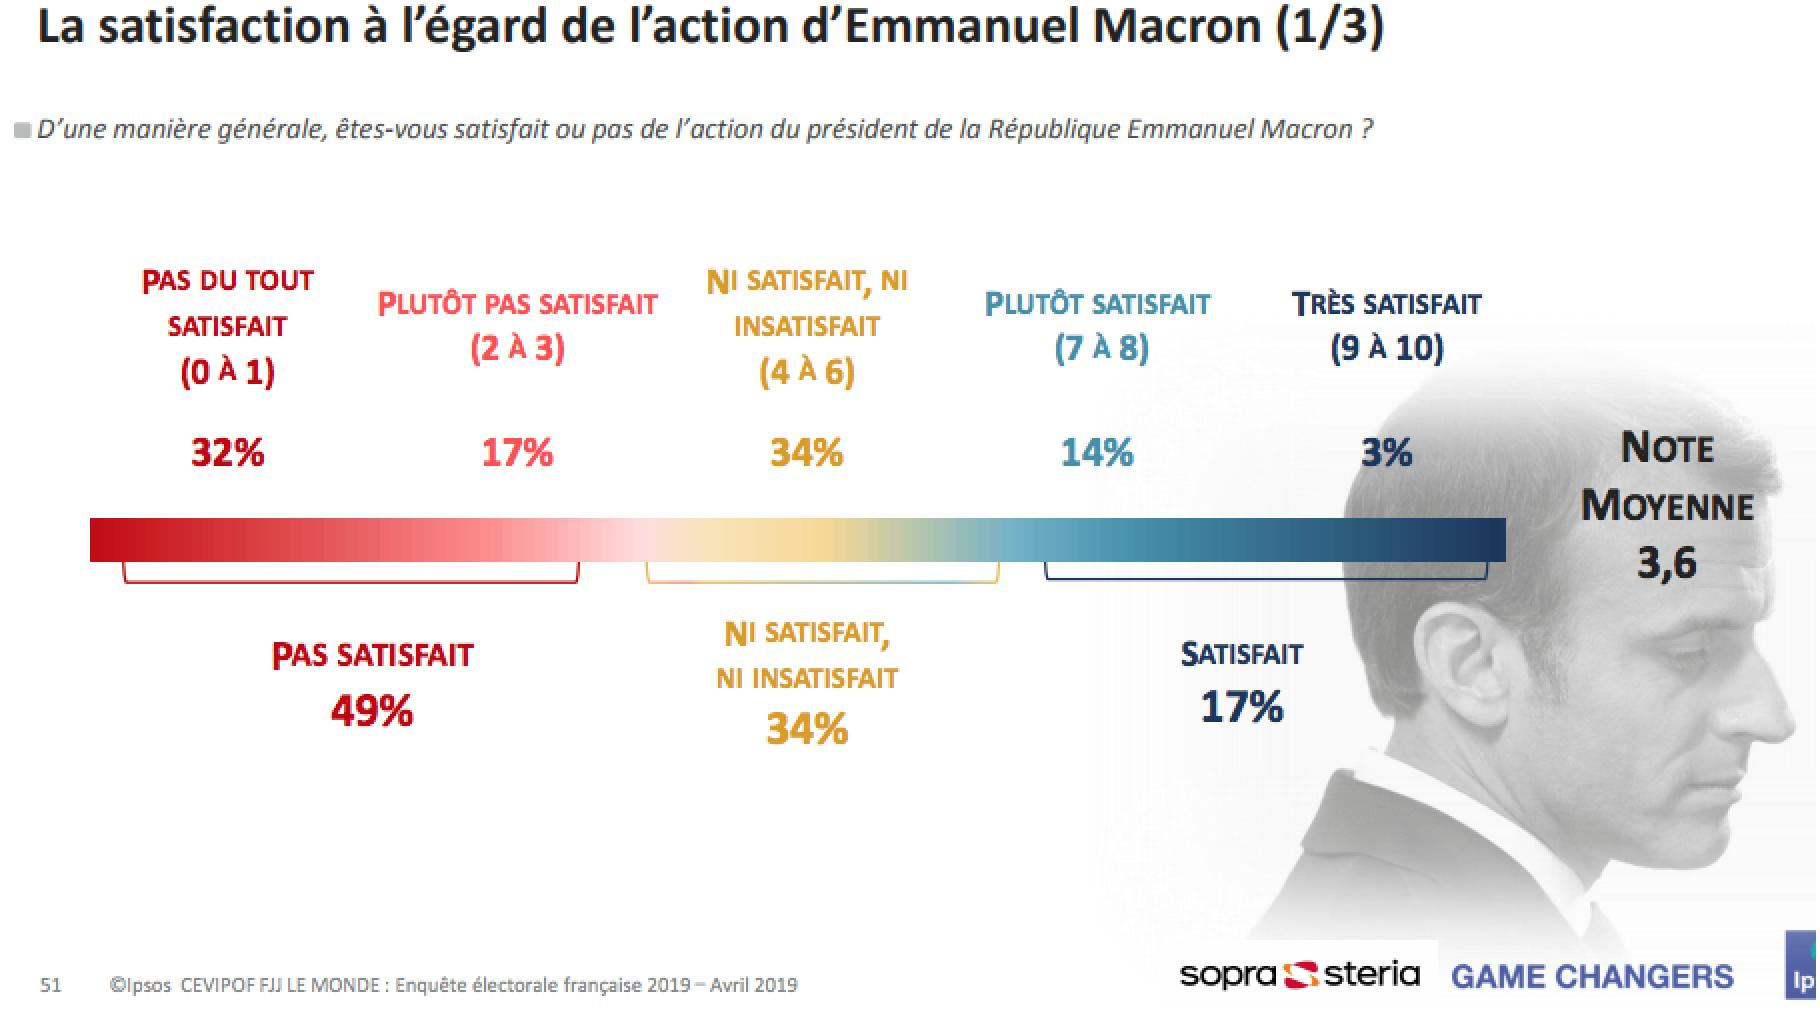
\includegraphics[width = 1.0\textwidth]{PopulariteMacron.jpg}}
   \only<2>{Corrigé}
   \only<2>{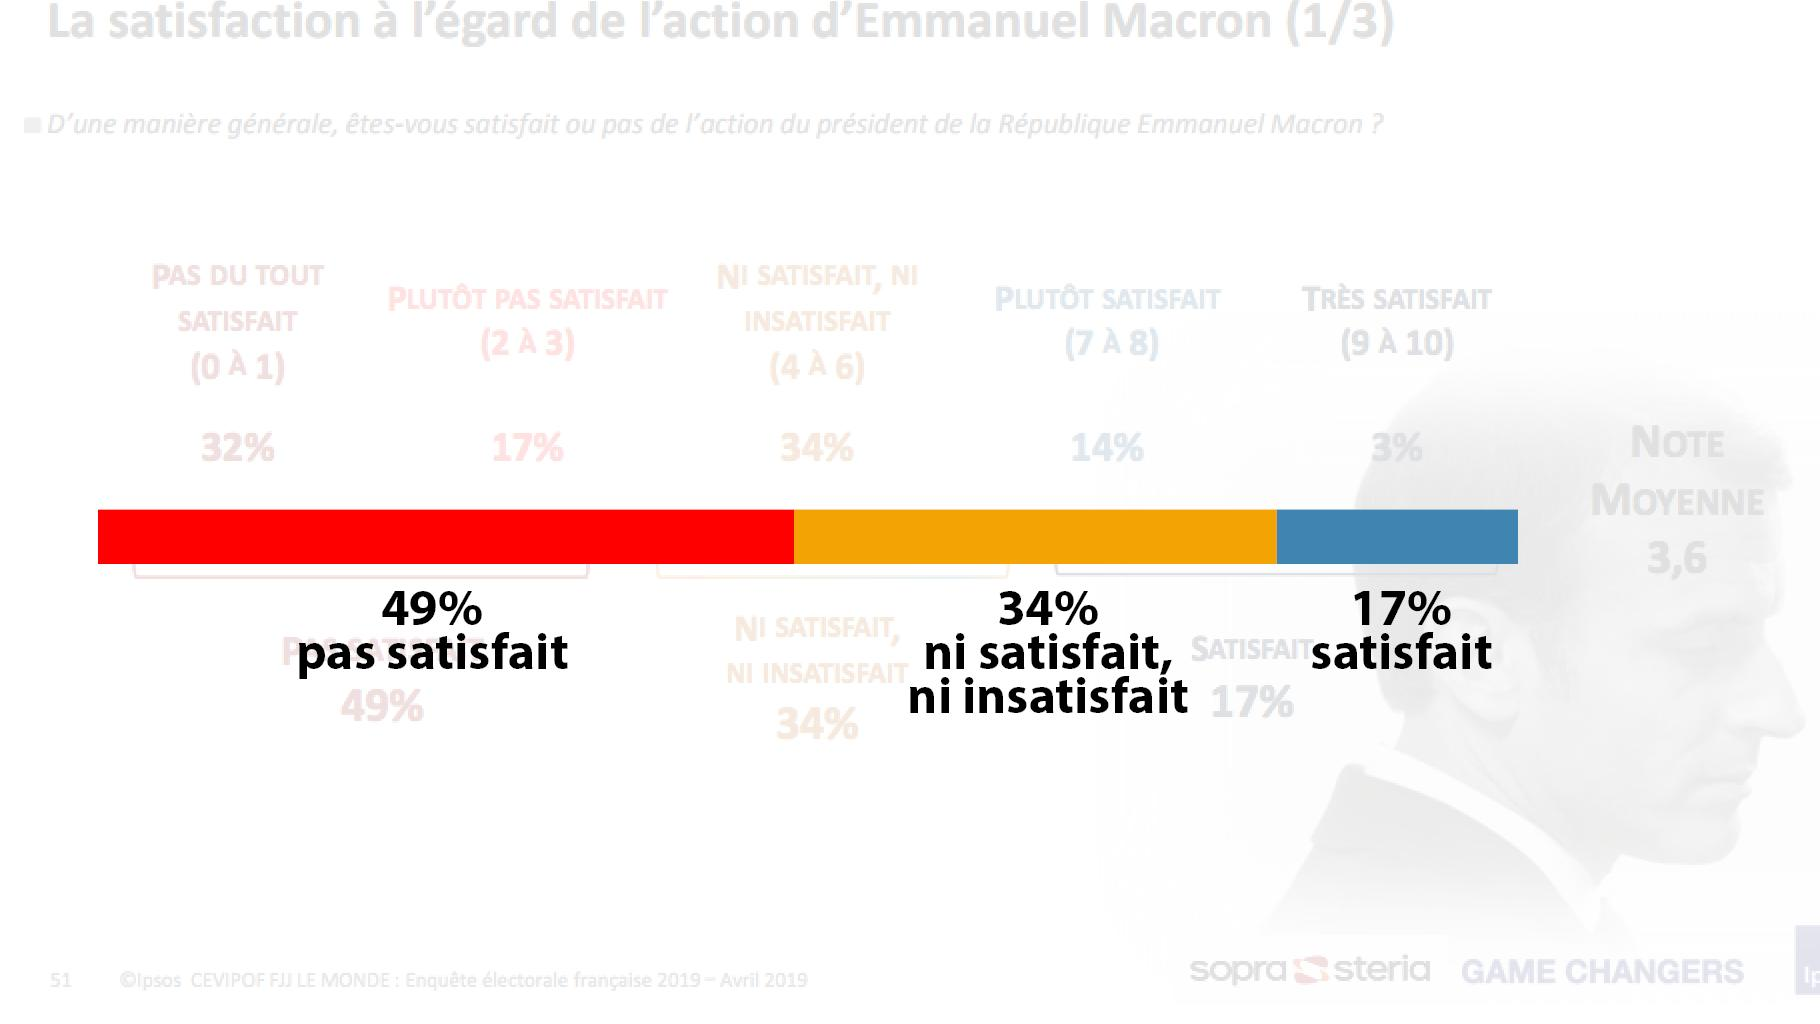
\includegraphics[width = 1.0\textwidth]{PopulariteMacronCorrigeNBoeuf.jpg}}
\end{enumerate}
\end{center}
\end{frame}

%% Elections UE-BBC
\begin{frame}
\frametitle{\textcolor{brique}{[- Be Subtle -]}}
\begin{center}
\begin{enumerate}
   \only<1>{Original}
   \only<1>{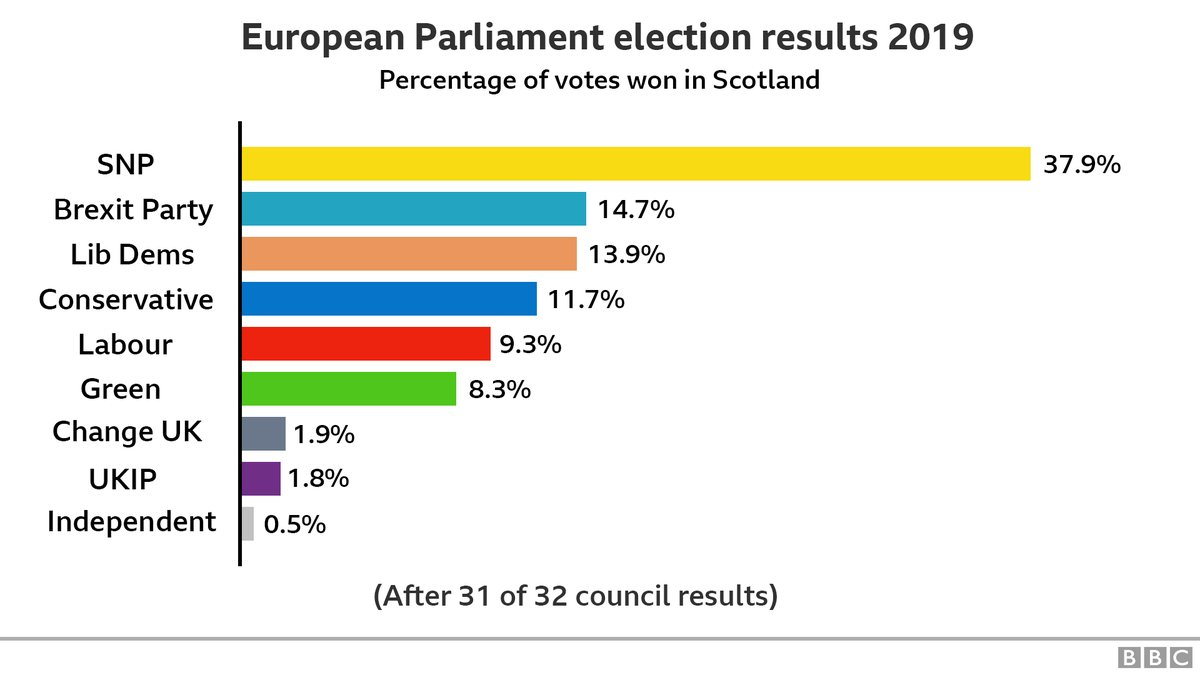
\includegraphics[width = 1.0\textwidth]{BBC-EUElectionOriginal.jpg}}
   \only<2>{Détection}
   \only<2>{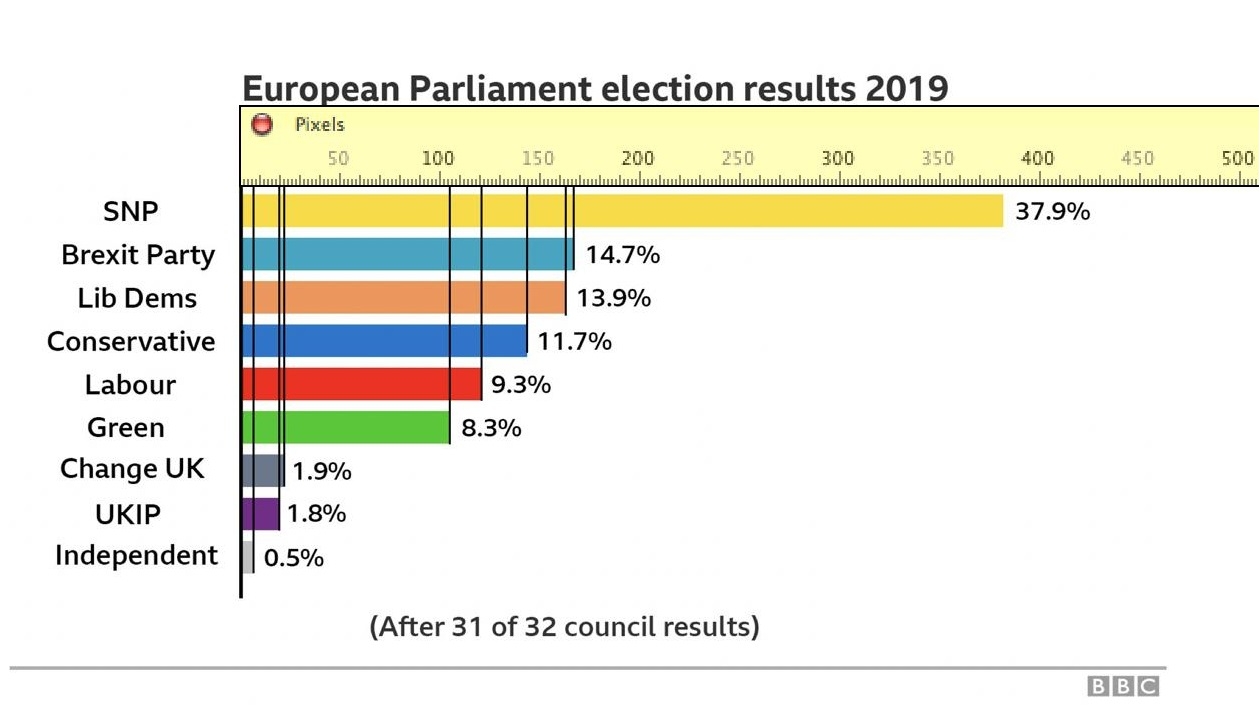
\includegraphics[width = 1.0\textwidth]{BBC-EUElectionLie2.jpg}}
   \only<3>{Correction}
   \only<3>{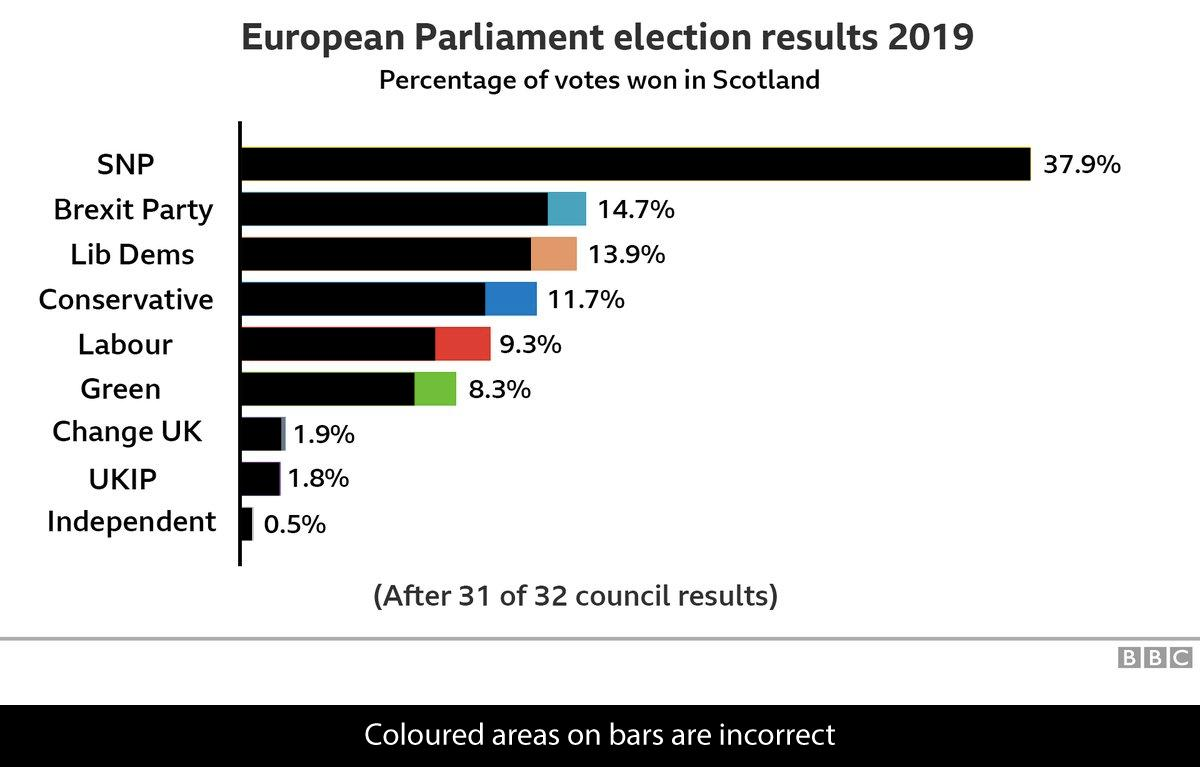
\includegraphics[width = 1.0\textwidth]{BBC-EUElectionCorrected1.jpg}}
   \only<4>{Vérification}
   \only<4>{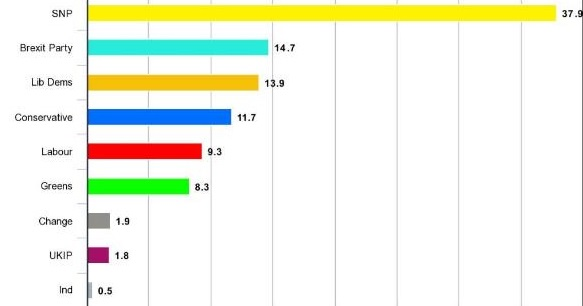
\includegraphics[width = 1.0\textwidth]{BBC-EUElectionCorrected3.jpg}}
\end{enumerate}
\end{center}
\end{frame}

% Indian Oil
\begin{frame}
\frametitle{\textcolor{brique}{[- Be Subtle (or not) -]}}
\begin{center}
\begin{enumerate}
   \only<1>{Original}
   \only<1>{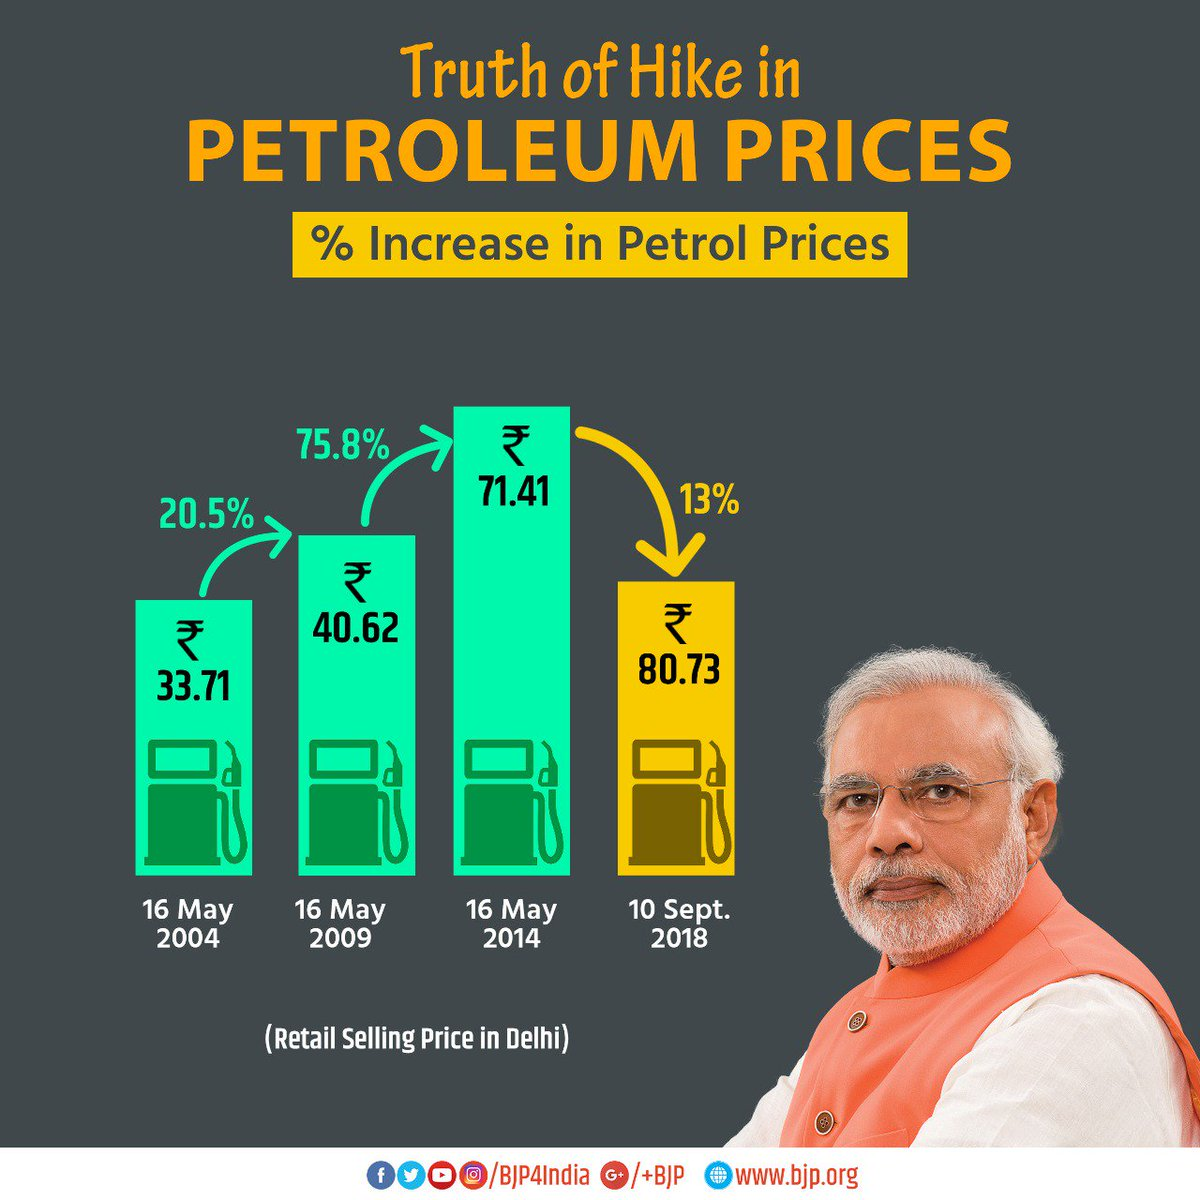
\includegraphics[width = 0.6\textwidth]{IndianPrimeMinisterPetrol2018.jpg}}
   \only<2>{LOL !}
   \only<2>{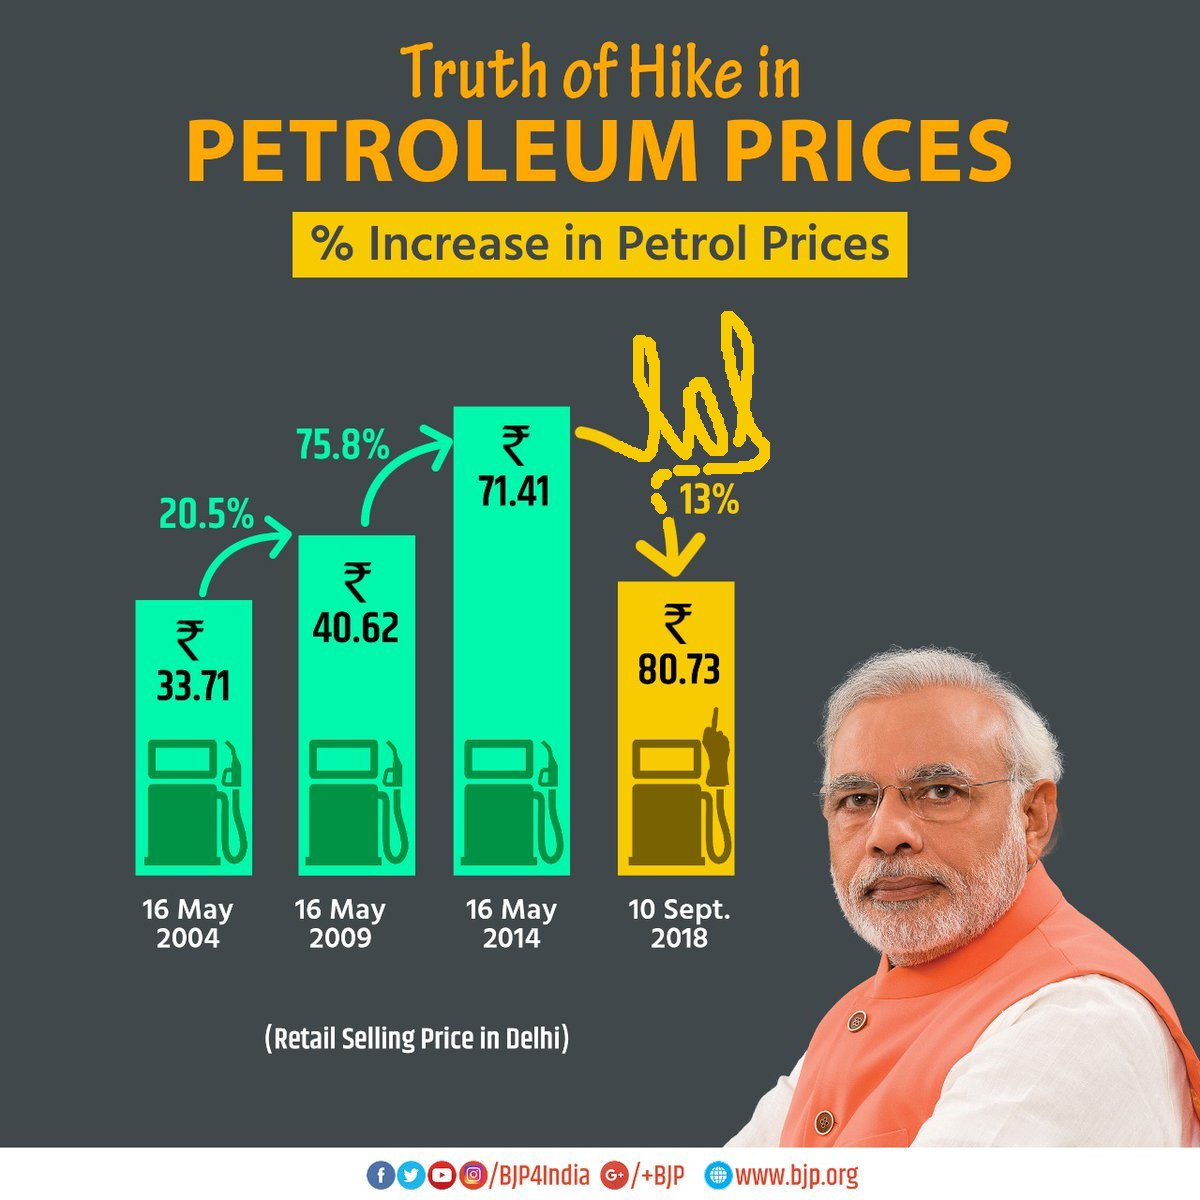
\includegraphics[width = 0.6\textwidth]{IndianPrimeMinisterPetrol2018_Lol.jpg}}
   \only<3>{Correction?}
   \only<3>{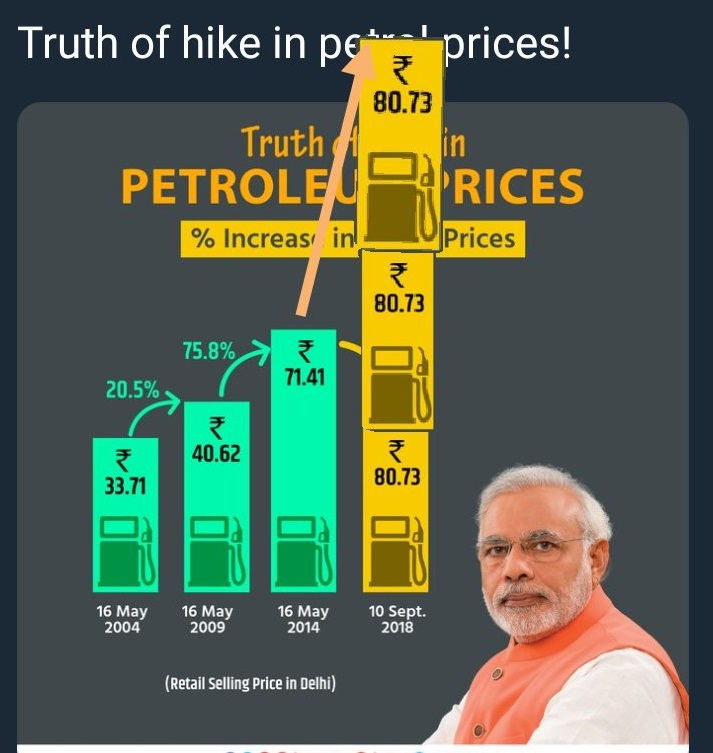
\includegraphics[width = 0.6\textwidth]{IndianPrimeMinisterPetrol2018_Corrected.jpg}}
   \only<4>{Justification!}
   \only<4>{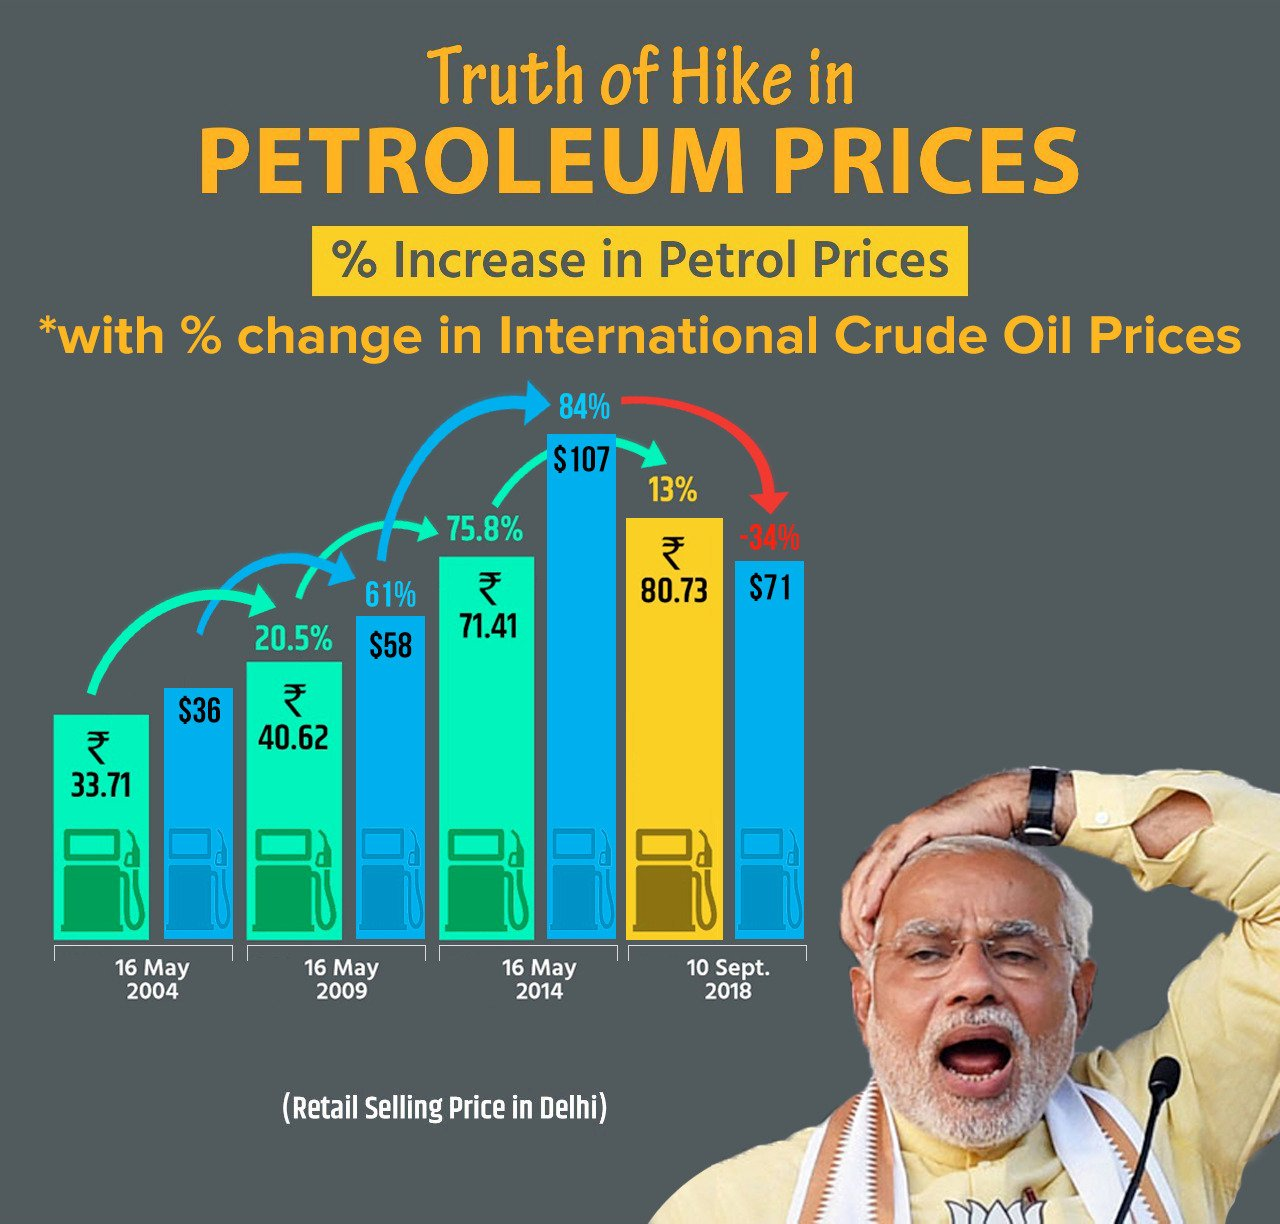
\includegraphics[width = 0.6\textwidth]{IndianPrimeMinisterPetrol2018_Corrected2.jpg}}
   \only<5>{LOL !}
   \only<5>{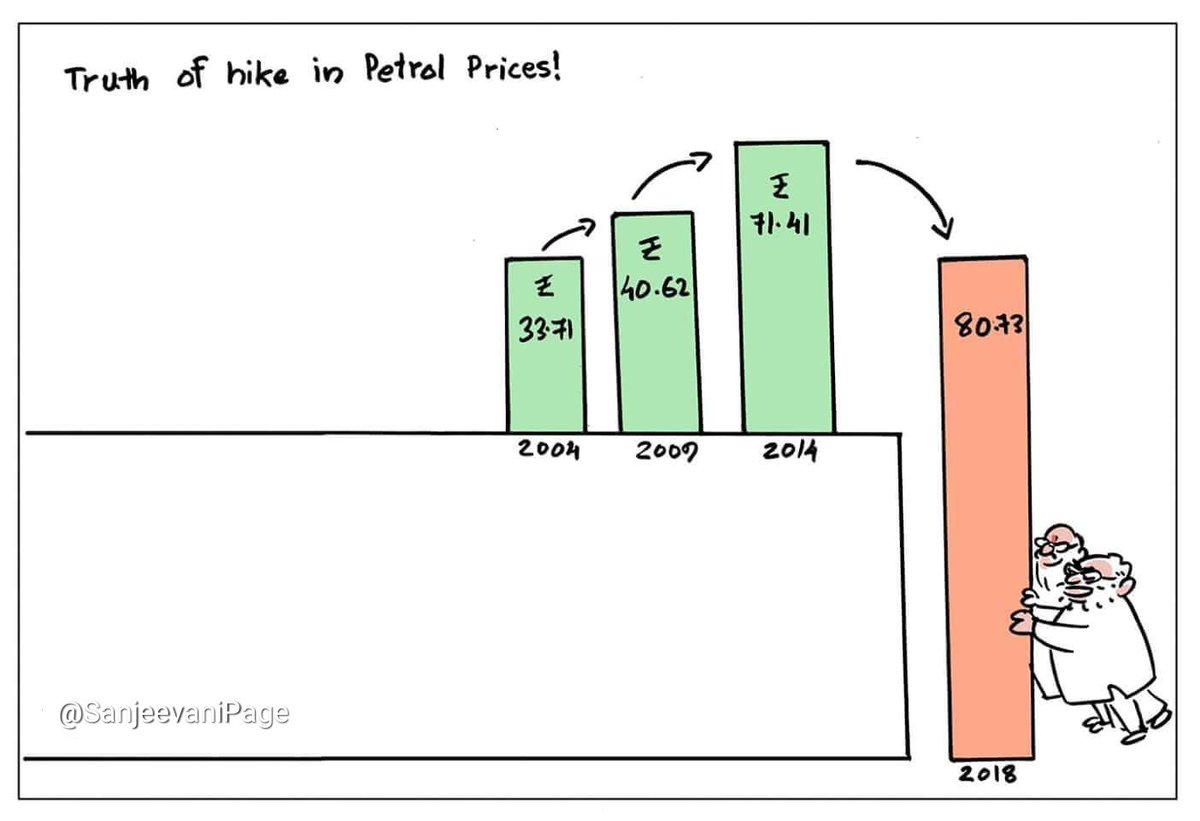
\includegraphics[width = 0.8\textwidth]{IndianPrimeMinisterPetrol2018_Lol2.jpg}}
\end{enumerate}
\end{center}
\end{frame}


\begin{frame}
\frametitle{\textcolor{brique}{[- Be Subtle (or not) -]}}
Les chiffres ne trompent pas...
\begin{center}
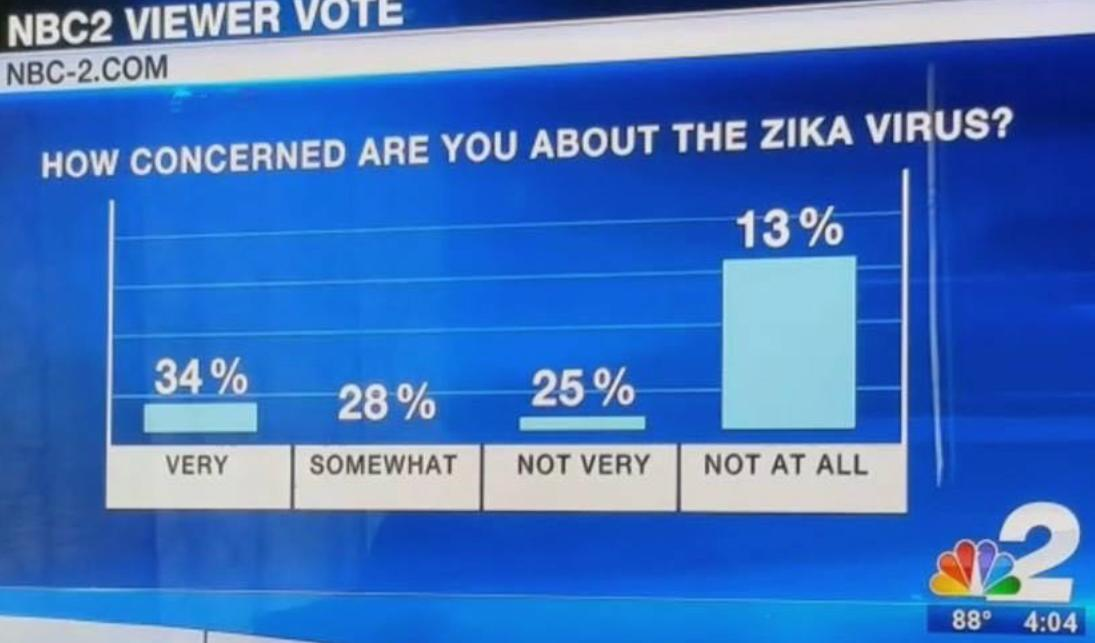
\includegraphics[width = 1.1\textheight]{CBSNZika.jpg}
\end{center}
\end{frame}





\end{document}

%%%%%%%%%%%%%%%%%%%%%%%%%%%%%%%%%%%%%%%%%%%%%%%%%%%%

%%%%%%%%%%%%%%%%%%%%%%%%%%%%%%%%%%%%%%%%%%%%%%%%%%%%
%%%%%%%%%%%%%%%%%%%%%%%%%%%%%%%%%%%%%%%%%%%%%%%%%%%%

